%%%%%%%%%%%%%%%%%%%%%%%%%%%%%%%%%%%%%%%%%
% The Legrand Orange Book
% LaTeX Template
% Version 2.1.1 (14/2/16)
%
% This template has been downloaded from:
% http://www.LaTeXTemplates.com
%
% Original author:
% Mathias Legrand (legrand.mathias@gmail.com) with modifications by:
% Vel (vel@latextemplates.com)
% Arne Eide
%
% License:
% CC BY-NC-SA 3.0 (http://creativecommons.org/licenses/by-nc-sa/3.0/)
%
% Compiling this template:
% This template uses biber (Mendely) for its bibliography and makeindex for its index.
% When you first open the template, compile it from the command line with the 
% commands below to make sure your LaTeX distribution is configured correctly:
%
% 1) pdflatex main
% 2) makeindex main.idx -s StyleInd.ist
% 3) biber main
% 4) pdflatex main x 2
%
% After this, when you wish to update the bibliography/index use the appropriate
% command above and make sure to compile with pdflatex several times 
% afterwards to propagate your changes to the document.
%
% This template also uses a number of packages which may need to be
% updated to the newest versions for the template to compile. It is strongly
% recommended you update your LaTeX distribution if you have any
% compilation errors.
%
% Important note:
% Chapter heading images should have a 2:1 width:height ratio,
% e.g. 920px width and 460px height.
%
%%%%%%%%%%%%%%%%%%%%%%%%%%%%%%%%%%%%%%%%%

%----------------------------------------------------------------------------------------
%	PACKAGES AND OTHER DOCUMENT CONFIGURATIONS
%----------------------------------------------------------------------------------------

\documentclass[11pt,fleqn]{book} % Default font size and left-justified equations

%%%%%%%%%%%%%%%%%%%%%%%%%%%%%%%%%%%%%%%%%
% The Legrand Orange Book
% Structural Definitions File
% Version 2.0 (9/2/15)
%
% Original author:
% Mathias Legrand (legrand.mathias@gmail.com) with modifications by:
% Vel (vel@latextemplates.com)
% 
% This file has been downloaded from:
% http://www.LaTeXTemplates.com
%
% License:
% CC BY-NC-SA 3.0 (http://creativecommons.org/licenses/by-nc-sa/3.0/)
%
%%%%%%%%%%%%%%%%%%%%%%%%%%%%%%%%%%%%%%%%%

%----------------------------------------------------------------------------------------
%	VARIOUS REQUIRED PACKAGES AND CONFIGURATIONS
%----------------------------------------------------------------------------------------

\usepackage[top=3cm,bottom=3cm,left=3cm,right=3cm,headsep=10pt,a4paper]{geometry} % Page margins

\usepackage{graphicx} % Required for including pictures
\graphicspath{{Pictures/}} % Specifies the directory where pictures are stored

\usepackage{lipsum} % Inserts dummy text

\usepackage{tikz} % Required for drawing custom shapes

\usepackage[english]{babel} % English language/hyphenation

\usepackage{enumitem} % Customize lists
\setlist{nolistsep} % Reduce spacing between bullet points and numbered lists

\usepackage{booktabs} % Required for nicer horizontal rules in tables

\usepackage{xcolor,colortbl} % Required for specifying colors by name
\definecolor{ocre}{RGB}{51, 102, 204} % Define the orange color used for highlighting throughout the book

\usepackage[section]{placeins} %Package to hold figures at fixed places
\usepackage{wrapfig} %Package to wrap around figures
\usepackage{sidecap} %Introduces SCfigure
\usepackage{caption}

\usepackage{floatrow}
\floatsetup[table]{capposition=top}

\usepackage{parskip}

%----------------------------------------------------------------------------------------
%	FONTS
%----------------------------------------------------------------------------------------

\usepackage{avant} % Use the Avantgarde font for headings
%\usepackage{times} % Use the Times font for headings

\usepackage{mathptmx}
 % Use the Adobe Times Roman as the default text font together with math symbols from the Sym­bol, Chancery and Com­puter Modern fonts

\usepackage{microtype} % Slightly tweak font spacing for aesthetics
\usepackage[utf8]{inputenc} % Required for including letters with accents
\usepackage[T1]{fontenc} % Use 8-bit encoding that has 256 glyphs
\usepackage{eurosym} % Eurosymbol
%----------------------------------------------------------------------------------------
%	BIBLIOGRAPHY AND INDEX
%----------------------------------------------------------------------------------------

\usepackage{csquotes}
\usepackage[style=numeric,citestyle=numeric,sorting=nyt,sortcites=true,autopunct=true,autolang=hyphen,hyperref=true,abbreviate=false,backref=true,backend=biber,defernumbers=true]{biblatex}
\addbibresource{Mendeley.bib} 
%\addbibresource{bibliography.bib} % BibTeX bibliography file
\defbibheading{bibempty}{}

\usepackage{calc} % For simpler calculation - used for spacing the index letter headings correctly
\usepackage{makeidx} % Required to make an index
\makeindex % Tells LaTeX to create the files required for indexing

%----------------------------------------------------------------------------------------
%	MAIN TABLE OF CONTENTS
%----------------------------------------------------------------------------------------

\usepackage{titletoc} % Required for manipulating the table of contents

\contentsmargin{0cm} % Removes the default margin

% Part text styling
\titlecontents{part}[0cm]
{\addvspace{20pt}\centering\large\bfseries}
{}
{}
{}

% Chapter text styling
\titlecontents{chapter}[1.25cm] % Indentation
{\addvspace{12pt}\large\sffamily\bfseries} % Spacing and font options for chapters
{\color{ocre!60}\contentslabel[\Large\thecontentslabel]{1.25cm}\color{ocre}} % Chapter number
{\color{ocre}}  
{\color{ocre!60}\normalsize\;\titlerule*[.5pc]{.}\;\thecontentspage} % Page number

% Section text styling
\titlecontents{section}[1.25cm] % Indentation
{\addvspace{3pt}\sffamily\bfseries} % Spacing and font options for sections
{\contentslabel[\thecontentslabel]{1.25cm}} % Section number
{}
{\hfill\color{black}\thecontentspage} % Page number
[]

% Subsection text styling
\titlecontents{subsection}[1.25cm] % Indentation
{\addvspace{1pt}\sffamily\small} % Spacing and font options for subsections
{\contentslabel[\thecontentslabel]{1.25cm}} % Subsection number
{}
{\ \titlerule*[.5pc]{.}\;\thecontentspage} % Page number
[]

% List of figures
\titlecontents{figure}[0em]
{\addvspace{-5pt}\sffamily}
{\thecontentslabel\hspace*{1em}}
{}
{\ \titlerule*[.5pc]{.}\;\thecontentspage}
[]

% List of tables
\titlecontents{table}[0em]
{\addvspace{-5pt}\sffamily}
{\thecontentslabel\hspace*{1em}}
{}
{\ \titlerule*[.5pc]{.}\;\thecontentspage}
[]

%----------------------------------------------------------------------------------------
%	MINI TABLE OF CONTENTS IN PART HEADS
%----------------------------------------------------------------------------------------

% Chapter text styling
\titlecontents{lchapter}[0em] % Indenting
{\addvspace{15pt}\large\sffamily\bfseries} % Spacing and font options for chapters
{\color{ocre}\contentslabel[\Large\thecontentslabel]{1.25cm}\color{ocre}} % Chapter number
{}  
{\color{ocre}\normalsize\sffamily\bfseries\;\titlerule*[.5pc]{.}\;\thecontentspage} % Page number

% Section text styling
\titlecontents{lsection}[0em] % Indenting
{\sffamily\small} % Spacing and font options for sections
{\contentslabel[\thecontentslabel]{1.25cm}} % Section number
{}
{}

% Subsection text styling
\titlecontents{lsubsection}[.5em] % Indentation
{\normalfont\footnotesize\sffamily} % Font settings
{}
{}
{}

%----------------------------------------------------------------------------------------
%	PAGE HEADERS
%----------------------------------------------------------------------------------------

\usepackage{fancyhdr} % Required for header and footer configuration

\pagestyle{fancy}
\renewcommand{\chaptermark}[1]{\markboth{\sffamily\normalsize\bfseries\chaptername\ \thechapter.\ #1}{}} % Chapter text font settings
\renewcommand{\sectionmark}[1]{\markright{\sffamily\normalsize\thesection\hspace{5pt}#1}{}} % Section text font settings
\fancyhf{} \fancyhead[LE,RO]{\sffamily\normalsize\thepage} % Font setting for the page number in the header
\fancyhead[LO]{\rightmark} % Print the nearest section name on the left side of odd pages
\fancyhead[RE]{\leftmark} % Print the current chapter name on the right side of even pages
\renewcommand{\headrulewidth}{0.5pt} % Width of the rule under the header
\addtolength{\headheight}{2.5pt} % Increase the spacing around the header slightly
\renewcommand{\footrulewidth}{0pt} % Removes the rule in the footer
\fancypagestyle{plain}{\fancyhead{}\renewcommand{\headrulewidth}{0pt}} % Style for when a plain pagestyle is specified

% Removes the header from odd empty pages at the end of chapters
\makeatletter
\renewcommand{\cleardoublepage}{
\clearpage\ifodd\c@page\else
\hbox{}
\vspace*{\fill}
\thispagestyle{empty}
\newpage
\fi}

%----------------------------------------------------------------------------------------
%	THEOREM STYLES
%----------------------------------------------------------------------------------------

\usepackage{amsmath,amsfonts,amssymb,amsthm,mmacells} % For math equations, theorems, symbols, etc

\newcommand{\intoo}[2]{\mathopen{]}#1\,;#2\mathclose{[}}
\newcommand{\ud}{\mathop{\mathrm{{}d}}\mathopen{}}
\newcommand{\intff}[2]{\mathopen{[}#1\,;#2\mathclose{]}}
\newtheorem{notation}{Notation}[chapter]

% Boxed/framed environments
\newtheoremstyle{ocrenumbox}% % Theorem style name
{0pt}% Space above
{0pt}% Space below
{\normalfont}% % Body font
{}% Indent amount
{\small\bf\sffamily\color{ocre}}% % Theorem head font
{\;}% Punctuation after theorem head
{0.25em}% Space after theorem head
{\small\sffamily\color{ocre}\thmname{#1}\nobreakspace\thmnumber{\@ifnotempty{#1}{}\@upn{#2}}% Theorem text (e.g. Theorem 2.1)
\thmnote{\nobreakspace\the\thm@notefont\sffamily\bfseries\color{black}---\nobreakspace#3.}} % Optional theorem note
\renewcommand{\qedsymbol}{$\blacksquare$}% Optional qed square

\newtheoremstyle{blacknumex}% Theorem style name
{5pt}% Space above
{5pt}% Space below
{\normalfont}% Body font
{} % Indent amount
{\small\bf\sffamily}% Theorem head font
{\;}% Punctuation after theorem head
{0.25em}% Space after theorem head
{\small\sffamily{\tiny\ensuremath{\blacksquare}}\nobreakspace\thmname{#1}\nobreakspace\thmnumber{\@ifnotempty{#1}{}\@upn{#2}}% Theorem text (e.g. Theorem 2.1)
\thmnote{\nobreakspace\the\thm@notefont\sffamily\bfseries---\nobreakspace#3.}}% Optional theorem note

\newtheoremstyle{blacknumbox} % Theorem style name
{0pt}% Space above
{0pt}% Space below
{\normalfont}% Body font
{}% Indent amount
{\small\bf\sffamily}% Theorem head font
{\;}% Punctuation after theorem head
{0.25em}% Space after theorem head
{\small\sffamily\thmname{#1}\nobreakspace\thmnumber{\@ifnotempty{#1}{}\@upn{#2}}% Theorem text (e.g. Theorem 2.1)
\thmnote{\nobreakspace\the\thm@notefont\sffamily\bfseries---\nobreakspace#3.}}% Optional theorem note

% Non-boxed/non-framed environments
\newtheoremstyle{ocrenum}% % Theorem style name
{5pt}% Space above
{5pt}% Space below
{\normalfont}% % Body font
{}% Indent amount
{\small\bf\sffamily\color{ocre}}% % Theorem head font
{\;}% Punctuation after theorem head
{0.25em}% Space after theorem head
{\small\sffamily\color{ocre}\thmname{#1}\nobreakspace\thmnumber{\@ifnotempty{#1}{}\@upn{#2}}% Theorem text (e.g. Theorem 2.1)
\thmnote{\nobreakspace\the\thm@notefont\sffamily\bfseries\color{black}---\nobreakspace#3.}} % Optional theorem note
\renewcommand{\qedsymbol}{$\blacksquare$}% Optional qed square
\makeatother

% Defines the theorem text style for each type of theorem to one of the three styles above
\newcounter{dummy} 
\numberwithin{dummy}{section}
\theoremstyle{ocrenumbox}
\newtheorem{theoremeT}[dummy]{Code box}
\newtheorem{problem}{Problem}[chapter]
\newtheorem{exerciseT}{Exercise}[chapter]
\theoremstyle{blacknumex}
\newtheorem{exampleT}{Example}[chapter]
\theoremstyle{blacknumbox}
\newtheorem{vocabulary}{Vocabulary}[chapter]
\newtheorem{definitionT}{Summary}[section]
\newtheorem{corollaryT}{Additional remarks}[chapter]
\theoremstyle{ocrenum}
\newtheorem{proposition}[dummy]{Proposition}

%----------------------------------------------------------------------------------------
%	DEFINITION OF COLORED BOXES
%----------------------------------------------------------------------------------------

\RequirePackage[framemethod=default]{mdframed} % Required for creating the theorem, definition, exercise and corollary boxes

% Theorem box  (Code box)
\newmdenv[skipabove=19pt,
skipbelow=7pt,
backgroundcolor=black!4,
linecolor=ocre,
innerleftmargin=5pt,
innerrightmargin=5pt,
innertopmargin=9pt,
leftmargin=0cm,
rightmargin=0cm,
innerbottommargin=5pt]{tBox}

% Exercise box	  
\newmdenv[skipabove=17pt,
skipbelow=2pt,
rightline=false,
leftline=true,
topline=false,
bottomline=false,
backgroundcolor=ocre!10,
linecolor=ocre,
innerleftmargin=5pt,
innerrightmargin=5pt,
innertopmargin=9pt,
innerbottommargin=5pt,
leftmargin=0cm,
rightmargin=0cm,
linewidth=4pt]{eBox}	

% Definition box (Summary)
\newmdenv[skipabove=19pt,
skipbelow=7pt,
rightline=false,
leftline=true,
topline=false,
bottomline=false,
linecolor=ocre,
innerleftmargin=5pt,
innerrightmargin=5pt,
innertopmargin=9pt,
leftmargin=0cm,
rightmargin=0cm,
linewidth=4pt,
innerbottommargin=0pt]{dBox}	

% Corollary box (Additional remarks)
\newmdenv[skipabove=19pt,
skipbelow=7pt,
rightline=false,
leftline=true,
topline=false,
bottomline=false,
linecolor=gray,
backgroundcolor=black!5,
innerleftmargin=5pt,
innerrightmargin=5pt,
innertopmargin=9pt,
leftmargin=0cm,
rightmargin=0cm,
linewidth=4pt,
innerbottommargin=5pt]{cBox}

% Creates an environment for each type of theorem and assigns it a theorem text style from the "Theorem Styles" section above and a colored box from above
\newenvironment{theorem}{\begin{tBox}\begin{theoremeT}}{\end{theoremeT}\end{tBox}}
\newenvironment{exercise}{\begin{eBox}\begin{exerciseT}}{\hfill{\color{ocre}\tiny\ensuremath{\blacksquare}}\end{exerciseT}\end{eBox}}				  
\newenvironment{definition}{\begin{dBox}\begin{definitionT}}{\end{definitionT}\end{dBox}}	
\newenvironment{example}{\begin{exampleT}}{\hfill{\tiny\ensuremath{\blacksquare}}\end{exampleT}}		
\newenvironment{corollary}{\begin{cBox}\begin{corollaryT}}{\end{corollaryT}\end{cBox}}	

%----------------------------------------------------------------------------------------
%	REMARK ENVIRONMENT
%----------------------------------------------------------------------------------------

\newenvironment{remark}{\par\vspace{10pt}\small % Vertical white space above the remark and smaller font size
\begin{list}{}{
\leftmargin=40pt % Indentation on the left
\rightmargin=25pt}\item\ignorespaces % Indentation on the right
\makebox[-2.5pt]{\begin{tikzpicture}[overlay]
\node[draw=ocre!60,line width=1pt,rectangle,fill=ocre!25,font=\sffamily\bfseries,inner sep=2pt,outer sep=0pt] at (-25pt,0pt){\textcolor{ocre}{DEMO}};\end{tikzpicture}} % Orange R in a circle
\advance\baselineskip -1pt}{\end{list}\vskip5pt} % Tighter line spacing and white space after remark

%----------------------------------------------------------------------------------------
%	SECTION NUMBERING IN THE MARGIN
%----------------------------------------------------------------------------------------

\makeatletter
\renewcommand{\@seccntformat}[1]{\llap{\textcolor{ocre}{\csname the#1\endcsname}\hspace{1em}}}                    
\renewcommand{\section}{\@startsection{section}{1}{\z@}
{-4ex \@plus -1ex \@minus -.4ex}
{1ex \@plus.2ex }
{\normalfont\large\sffamily\bfseries}}
\renewcommand{\subsection}{\@startsection {subsection}{2}{\z@}
{-3ex \@plus -0.1ex \@minus -.4ex}
{0.5ex \@plus.2ex }
{\normalfont\sffamily\bfseries}}
\renewcommand{\subsubsection}{\@startsection {subsubsection}{3}{\z@}
{-2ex \@plus -0.1ex \@minus -.2ex}
{.2ex \@plus.2ex }
{\normalfont\small\sffamily\bfseries}}                        
\renewcommand\paragraph{\@startsection{paragraph}{4}{\z@}
{-2ex \@plus-.2ex \@minus .2ex}
{.1ex}
{\normalfont\small\sffamily\bfseries}}

%----------------------------------------------------------------------------------------
%	PART HEADINGS
%----------------------------------------------------------------------------------------

% numbered part in the table of contents
\newcommand{\@mypartnumtocformat}[2]{%
\setlength\fboxsep{0pt}%
\noindent\colorbox{ocre!20}{\strut\parbox[c][.7cm]{\ecart}{\color{ocre!70}\Large\sffamily\bfseries\centering#1}}\hskip\esp\colorbox{ocre!40}{\strut\parbox[c][.7cm]{\linewidth-\ecart-\esp}{\Large\sffamily\centering#2}}}%
%%%%%%%%%%%%%%%%%%%%%%%%%%%%%%%%%%
% unnumbered part in the table of contents
\newcommand{\@myparttocformat}[1]{%
\setlength\fboxsep{0pt}%
\noindent\colorbox{ocre!40}{\strut\parbox[c][.7cm]{\linewidth}{\Large\sffamily\centering#1}}}%
%%%%%%%%%%%%%%%%%%%%%%%%%%%%%%%%%%
\newlength\esp
\setlength\esp{4pt}
\newlength\ecart
\setlength\ecart{1.2cm-\esp}
\newcommand{\thepartimage}{}%
\newcommand{\partimage}[1]{\renewcommand{\thepartimage}{#1}}%
\def\@part[#1]#2{%
\ifnum \c@secnumdepth >-2\relax%
\refstepcounter{part}%
\addcontentsline{toc}{part}{\texorpdfstring{\protect\@mypartnumtocformat{\thepart}{#1}}{\partname~\thepart\ ---\ #1}}
\else%
\addcontentsline{toc}{part}{\texorpdfstring{\protect\@myparttocformat{#1}}{#1}}%
\fi%
\startcontents%
\markboth{}{}%
{\thispagestyle{empty}%
\begin{tikzpicture}[remember picture,overlay]%
\node at (current page.north west){\begin{tikzpicture}[remember picture,overlay]%	
\fill[ocre!20](0cm,0cm) rectangle (\paperwidth,-\paperheight);
\node[anchor=north] at (4cm,-3.25cm){\color{ocre!40}\fontsize{220}{100}\sffamily\bfseries\@Roman\c@part};    % arabic or Roman ------------------------
\node[anchor=south east] at (\paperwidth-1cm,-\paperheight+1cm){\parbox[t][][t]{8.5cm}{
\printcontents{l}{0}{\setcounter{tocdepth}{1}}%
}};
\node[anchor=north east] at (\paperwidth-1.5cm,-3.25cm){\parbox[t][][t]{15cm}{\strut\raggedleft\color{white}\fontsize{30}{30}\sffamily\bfseries#2}};
\end{tikzpicture}};
\end{tikzpicture}}%
\@endpart}
\def\@spart#1{%
\startcontents%
\phantomsection
{\thispagestyle{empty}%
\begin{tikzpicture}[remember picture,overlay]%
\node at (current page.north west){\begin{tikzpicture}[remember picture,overlay]%	
\fill[ocre!20](0cm,0cm) rectangle (\paperwidth,-\paperheight);
\node[anchor=north east] at (\paperwidth-1.5cm,-3.25cm){\parbox[t][][t]{15cm}{\strut\raggedleft\color{white}\fontsize{30}{30}\sffamily\bfseries#1}};
\end{tikzpicture}};
\end{tikzpicture}}
\addcontentsline{toc}{part}{\texorpdfstring{%
\setlength\fboxsep{0pt}%
\noindent\protect\colorbox{ocre!40}{\strut\protect\parbox[c][.7cm]{\linewidth}{\Large\sffamily\protect\centering #1\quad\mbox{}}}}{#1}}%
\@endpart}
\def\@endpart{\vfil\newpage
\if@twoside
\if@openright
\null
\thispagestyle{empty}%
\newpage
\fi
\fi
\if@tempswa
\twocolumn
\fi}

%----------------------------------------------------------------------------------------
%	CHAPTER HEADINGS
%----------------------------------------------------------------------------------------

% A switch to conditionally include a picture, implemented by  Christian Hupfer
\newif\ifusechapterimage
\usechapterimagetrue
\newcommand{\thechapterimage}{}%
\newcommand{\chapterimage}[1]{\ifusechapterimage\renewcommand{\thechapterimage}{#1}\fi}%
\def\@makechapterhead#1{%
{\parindent \z@ \raggedright \normalfont
\ifnum \c@secnumdepth >\m@ne
\if@mainmatter
\begin{tikzpicture}[remember picture,overlay]
\node at (current page.north west)
{\begin{tikzpicture}[remember picture,overlay]
\node[anchor=north west,inner sep=0pt] at (0,0) {\ifusechapterimage\includegraphics[width=\paperwidth]{\thechapterimage}\fi};
\draw[anchor=west] (\Gm@lmargin,-9cm) node [line width=2pt,rounded corners=15pt,draw=ocre,fill=white,fill opacity=0.5,inner sep=15pt]{\strut\makebox[22cm]{}};
\draw[anchor=west] (\Gm@lmargin+.3cm,-9cm) node {\huge\sffamily\bfseries\color{black}\thechapter. #1\strut};
\end{tikzpicture}};
\end{tikzpicture}
\else
\begin{tikzpicture}[remember picture,overlay]
\node at (current page.north west)
{\begin{tikzpicture}[remember picture,overlay]
\node[anchor=north west,inner sep=0pt] at (0,0) {\ifusechapterimage\includegraphics[width=\paperwidth]{\thechapterimage}\fi};
\draw[anchor=west] (\Gm@lmargin,-9cm) node [line width=2pt,rounded corners=15pt,draw=ocre,fill=white,fill opacity=0.5,inner sep=15pt]{\strut\makebox[22cm]{}};
\draw[anchor=west] (\Gm@lmargin+.3cm,-9cm) node {\huge\sffamily\bfseries\color{black}#1\strut};
\end{tikzpicture}};
\end{tikzpicture}
\fi\fi\par\vspace*{270\p@}}}

%-------------------------------------------

\def\@makeschapterhead#1{%
\begin{tikzpicture}[remember picture,overlay]
\node at (current page.north west)
{\begin{tikzpicture}[remember picture,overlay]
\node[anchor=north west,inner sep=0pt] at (0,0) {\ifusechapterimage\includegraphics[width=\paperwidth]{\thechapterimage}\fi};
\draw[anchor=west] (\Gm@lmargin,-9cm) node [line width=2pt,rounded corners=15pt,draw=ocre,fill=white,fill opacity=0.5,inner sep=15pt]{\strut\makebox[22cm]{}};
\draw[anchor=west] (\Gm@lmargin+.3cm,-9cm) node {\huge\sffamily\bfseries\color{black}#1\strut};
\end{tikzpicture}};
\end{tikzpicture}
\par\vspace*{270\p@}}
\makeatother

%----------------------------------------------------------------------------------------
%	HYPERLINKS IN THE DOCUMENTS
%----------------------------------------------------------------------------------------

\usepackage{hyperref}
\hypersetup{hidelinks,colorlinks=false,breaklinks=true,urlcolor= ocre,bookmarksopen=false,pdftitle={Title},pdfauthor={Author}}
\usepackage{bookmark}
\bookmarksetup{
open,
numbered,
addtohook={%
\ifnum\bookmarkget{level}=0 % chapter
\bookmarksetup{bold}%
\fi
\ifnum\bookmarkget{level}=-1 % part
\bookmarksetup{color=ocre,bold}%
\fi
}
}

%----------------------------------------------------------------------------------------
%	MMACELLS
%----------------------------------------------------------------------------------------

\usepackage[utf8]{inputenc}
\usepackage[T1]{fontenc}
\usepackage{lmodern}
\usepackage{mmacells}

\usepackage{tcolorbox}

\usepackage{multirow} % Insert the commands.tex file which contains the majority of the structure behind the template

\begin{document}

%\setlength{\parskip}{1em}

%----------------------------------------------------------------------------------------
%	MATHEMATICA CODES
%----------------------------------------------------------------------------------------

\mmaSet{uselistings=false}
% Use mmaUnd{}
\mmaDefineMathReplacement[≤]{<=}{\leq}
\mmaDefineMathReplacement[≥]{>=}{\geq}
\mmaDefineMathReplacement[≠]{!=}{\neq}
\mmaDefineMathReplacement[→]{->}{\to}[2]
\mmaDefineMathReplacement[⧴]{:>}{:\hspace{-.2em}\to}[2]
\mmaDefineMathReplacement{∉}{\notin}
\mmaDefineMathReplacement{∞}{\infty}
\mmaDefineMathReplacement{}{\mathbbm{d}}
\mmaDefineMathReplacement{ρ}{$\rho$}
\mmaDefineMathReplacement{λ}{$\lambda$}
\mmaDefineMathReplacement{±}{\pm}
\mmaDefineMathReplacement{α}{$\alpha$}
\mmaDefineMathReplacement{β}{$\beta$}
\mmaDefineMathReplacement{γ}{$\gamma$}

\mmaSet{morefv={gobble=2}}

%----------------------------------------------------------------------------------------
%	TITLE PAGE
%----------------------------------------------------------------------------------------

\begingroup
\thispagestyle{empty}
\begin{tikzpicture}[remember picture,overlay]
\coordinate [below=7cm] (midpoint) at (current page.north);
\node at (current page.north west)
{\begin{tikzpicture}[remember picture,overlay]
\node[anchor=north west,inner sep=0pt] at (0,0) {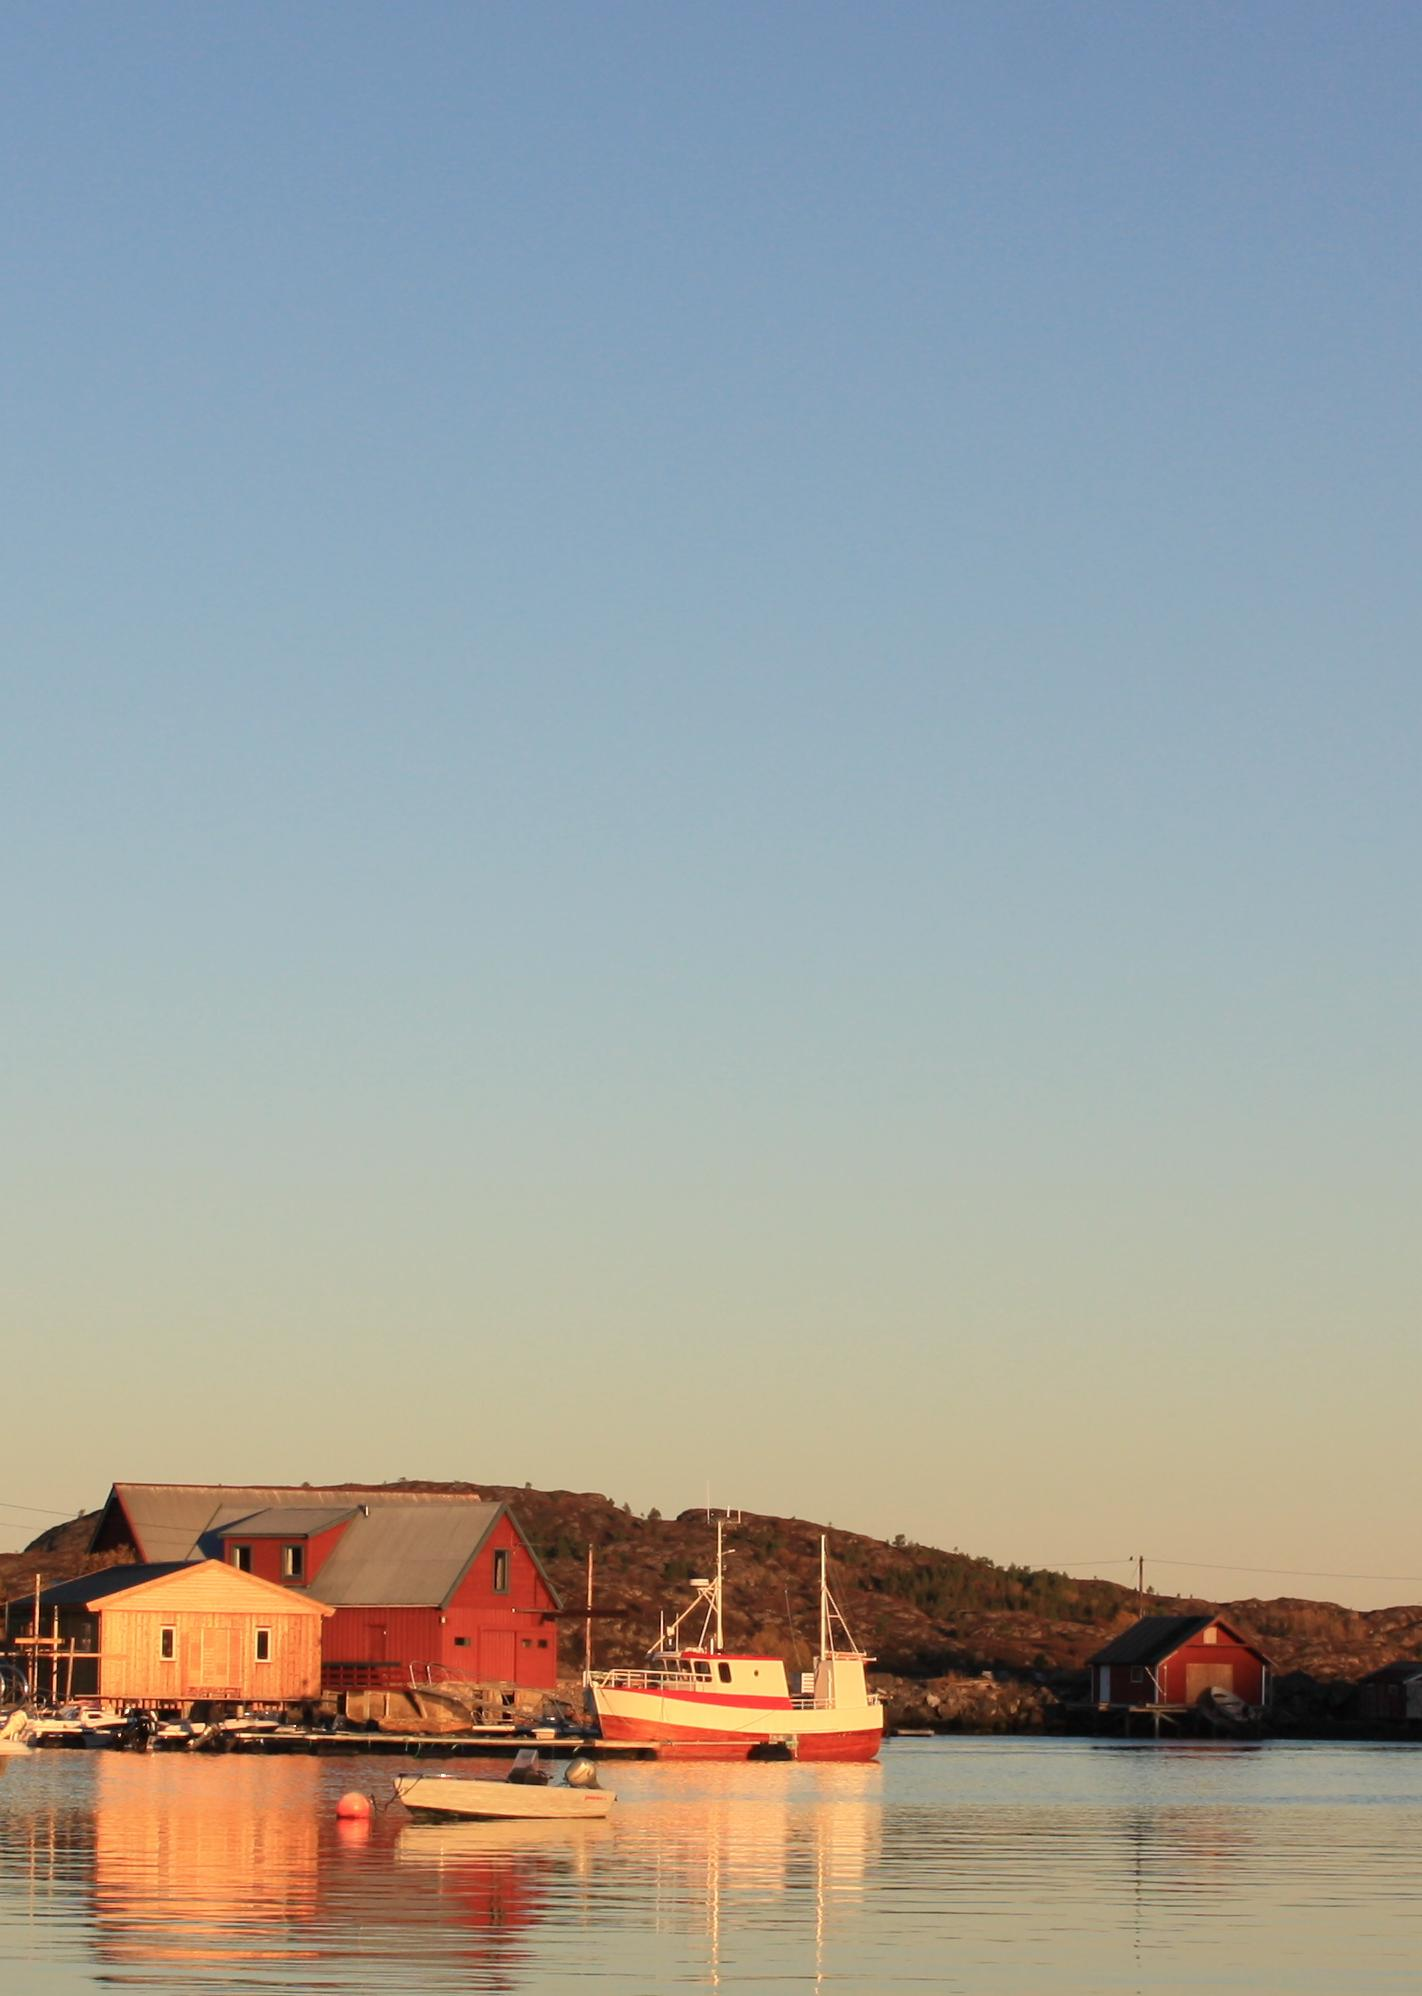
\includegraphics[width=\paperwidth]{cover4}}; % Background image
\draw[anchor=north] (midpoint) node [fill=ocre!30!white,fill opacity=0.6,text opacity=1,inner sep=1cm]{\Huge\centering\bfseries\sffamily\parbox[c][][t]{\paperwidth}{\centering Introduction to Fisheries Economics\\[15pt] % Book title
{\Large by the use of \textit{Wolfram Language} and \textit{Mathematica}}\\[20pt] % Subtitle
{\huge Arne Eide}}}; % Author name
\end{tikzpicture}};
\end{tikzpicture}
\vfill
\endgroup

%----------------------------------------------------------------------------------------
%	COPYRIGHT PAGE
%----------------------------------------------------------------------------------------

\newpage
~\vfill
\thispagestyle{empty}
\noindent Copyright \copyright\ 2020 Arne Eide % Copyright notice

\noindent \textsc{Published by Arne Eide} % Publisher

\noindent \textsc{doi: 10.6084/m9.figshare.3784821} % DOI

%\noindent \textsc{https://figshare.com/articles/Introduction\_to\_Fisheries\_Economics/3784821}\\ % URL
\noindent Licensed under the Creative Commons Attribution-NonCommercial 3.0 Unported License (the ``License''). You may not use this file (available at \url{https://figshare.com/articles/Introduction\_to\_Fisheries\_Economics/3784821}) except in compliance with the License. You may obtain a copy of the License at \url{http://creativecommons.org/licenses/by-nc/3.0}. Unless required by applicable law or agreed to in writing, software distributed under the License is distributed on an \textsc{``as is'' basis, without warranties or conditions of any kind}, either express or implied. See the License for the specific language governing permissions and limitations under the License.\\ % License information
\noindent \textit{Version 0.45, March 2020} % Printing/edition date

%----------------------------------------------------------------------------------------
%	TABLE OF CONTENTS
%----------------------------------------------------------------------------------------

%\usechapterimagefalse % If you don't want to include a chapter image, use this to toggle images off - it can be enabled later with \usechapterimagetrue

\chapterimage{wordcloud} % Table of contents heading image
%------------------------------------------------
\pagestyle{empty} % No headers
\tableofcontents % Print the table of contents itself
\cleardoublepage % Forces the first chapter to start on an odd page so it's on the right
\pagestyle{fancy} % Print headers again
\chapterimage{hintro.jpg} % Chapter heading image
%------------------------------------------------
\chapter{Introduction}\label{chapter 1}
Fishing, hunting and gathering food represent the oldest human forms of life, where people depended on wild food for subsistence. While the importance of hunting and gathering wild food decreased after the introduction of agriculture more than ten thousand years ago, fishing has over the last hundred years been increasingly more important as a source of food and wealth for millions of people around the world.

Fishing is an economic activity to produce food for own consumption, for accessing commercial markets for income, and for the purpose of recreation and pastime. These activities often coexist but could also be regarded as stages in economic and cultural developments, starting with the subsistence fishery, before developing a commercial industry and recreational use of the natural resource.

The aim of the earliest stage, the subsistence fishing, was to feed own household. Early barter economies allowed fish products to be traded. But as a perishable product there were limits for the trade-ability of fish. Methods to preserve fish by drying, salting and smoking it -- contributing in developing fish markets where stored fish could be sold -- were discovered and developed. Infrastructure became the major obstacle. Storing capacity, roads, vehicles for transport -- but also organisations, agreements and security trade investments -- were needed for transporting fish to markets in the large cities.

Increased demand and trade resulted in wealth creation, first in the secondary trading and later increasingly among fishers. One consequence of economic growth is that labour becomes more expensive and capital more accessible. Hence, if possible, labour is substituted by capital. The fishing industry is no exception.

The aim of recreational fishing, presumably the most recent commercial utilisation of fish stock resources, is not primarily to produce catch as catch is merely a mean to achieve the fishing experience. The ultimate goal is the adventure, utilising and enjoying the natural environment, sensing peaceful nature and experiencing relaxing activities. Recreational fishing has developed to become a major industry both in terms of accommodating game fishers, recreational activities and production of fishing tackle and equipment.

Fishing takes different forms in different societal and economic contexts. This book aims to discuss the economic activity of fishing through formal models while including the dynamics of the utilised fish stocks. The analysis are based on basic microeconomic principles, and standard theories of fisheries biology and economics. 

\section{What is a \textit{good} model?}\label{goodmodel}
A model is a generic term covering a large range of possible ways of simplifying, emphasising, exaggerating or clarifying complex matter. Graphical models, mathematical models and conceptual model represent different approaches, all aiming to reveal structures, patterns and coherence that are difficult to obtain without a modelling effort. If a model is a simplification of the real world it is of course untrue in the sense that it does not represent the full truth, some elements are missing. That is the whole point of employing models. Hence, a model could never be tested on being true or not, in some sense it is always untrue. The only criteria of the goodness of a model is: Is the model useful?

In figure~\ref{fig:globe} two different graphical models are shown. Which one is most useful depends solely on which problem we seek to solve. None will claim a street map to be at better model than a globe in general, it certainly depends on the problem we will solve. A globe is a better tool if we look at for example distances between large cities in different countries. For this purpose a street map is useless. This does not make a street map a bad model. The close link between the problem we are investigating and the model we use in this investigation is sometimes forgotten. But there is none general purpose model that can be used on all problems, -- unfortunately. We have to customise models for the specific problems we want to look into. This also goes to problems within the area in fisheries economics. This book therefore presents a range of different modelling approaches which all may be useful, -- given different problems.

\begin{figure}[ht]
\centering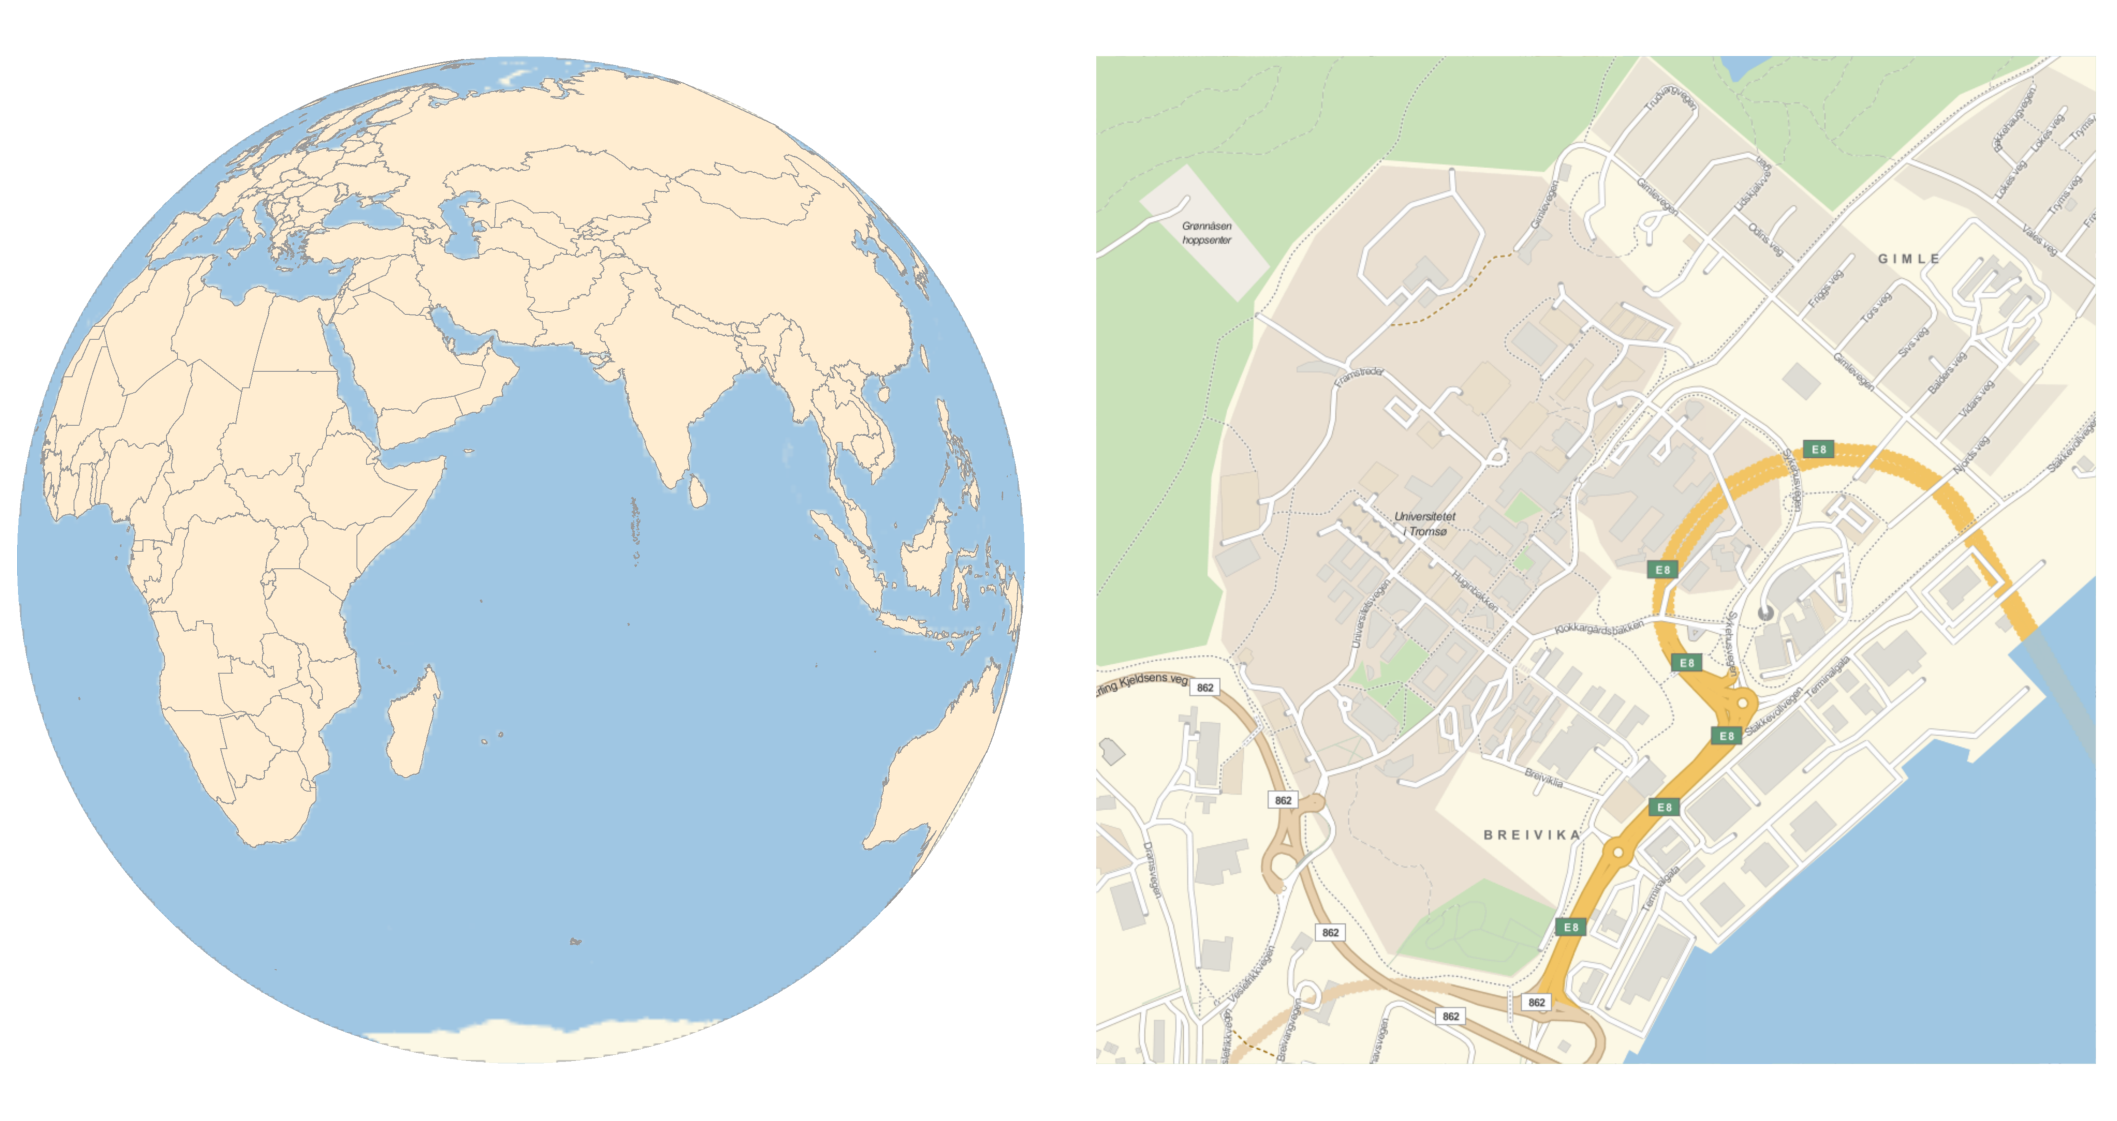
\includegraphics[scale=.4]{globe} 
\caption{Two models utilising geographical maps, a globe to the left and a street map to the right.\\}
\label{fig:globe}
\end{figure}

Research problems are expressed on basis of available data and knowledge we find relevant. When the problem is expressed we can construct a method -- or model -- we believe can highlight the problem and possibly solve it. Figure~\ref{fig:model} shows how the modelling process may be presented as a flow chart. The flow chart is a model of a general modelling process.

We note that a model has to be based on certain assumptions and that both the assumptions and the model expressions are closely linked to available knowledge (empirical and theoretical knowledge) and the the expressed problem initiating the process. Using the model we will gain results of some kind. The result of the modelling process is not the solution of the problem but one step in the direction of solving it. The most important process takes place in the green box in Figure~\ref{fig:model}.

When we analyse the modelling results we need to take into considerations the properties of the model, the assumptions we have made and relevant knowledge we did not include in the model. If the modelling effort has been successful we will gain knowledge after having analysed the results. By the new knowledge we may be able o express the research question more precisely and refine the model correspondingly. The modelling process therefore is an iterative process where it is possible to gain knowledge simply by looking more thoroughly on the knowledge we already had before starting the process.

This book presents several mathematical fishery models, aiming to capture population growth and fisheries economics. In many cases the specific problem leading to the chosen model remains vague or unexpressed. 

\begin{figure}[ht]
\centering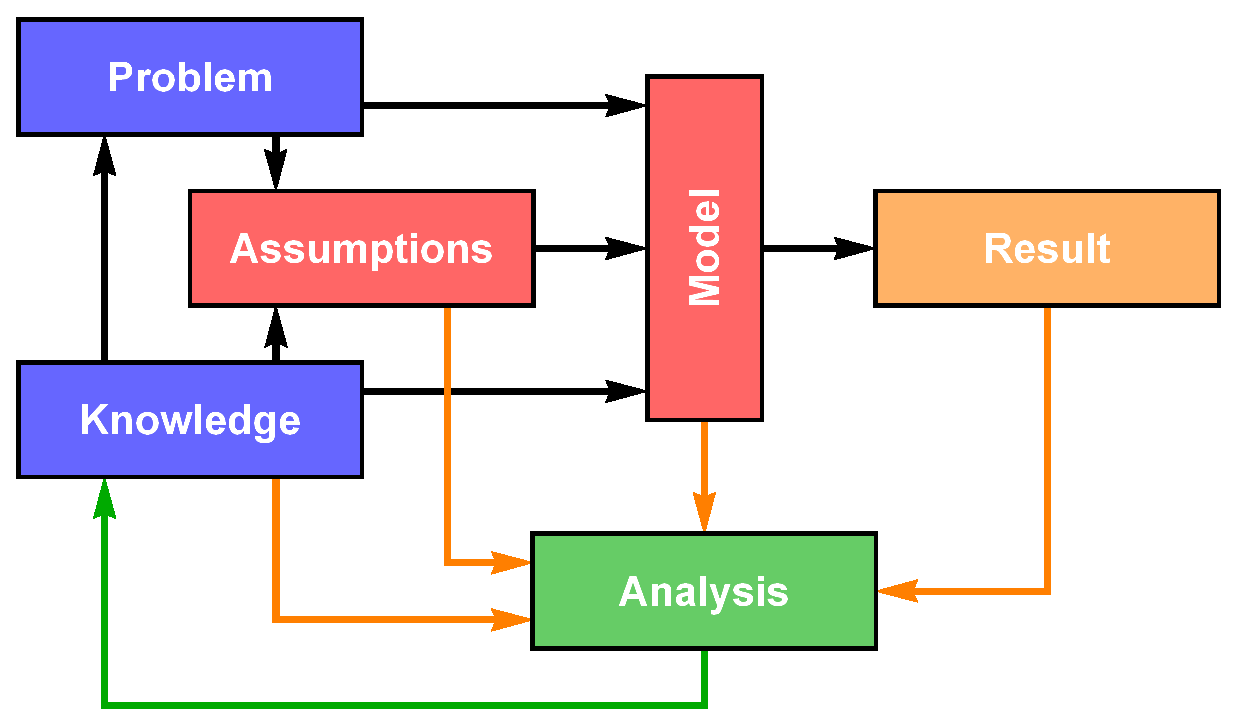
\includegraphics[scale=.6]{model} 
\caption{Flow chart of the iterative modelling process.}
\label{fig:model}
\end{figure}

\begin{definition}[What is a good model?]
A model \textit{useful} to highlight a specific problem is a \textit{good} model for that specific purpose. Another problem may be better solved by another model, useful for the investigation of that particular problem. There is no such thing as a true model, a good model is a model that is useful for the problem in question.
\end{definition}

\section{Interactive use of the codes in the book}
This book also offers simple programming codes written in the Wolfram Language (\textit{WL}), presenting relevant examples on how to use the software \textit{Mathematica} as a tool of modelling fisheries. Most of the figures displayed in the book is produced in Mathematica and the programming code is provided in the end of the book. In order to learn the basics of \textit{Mathematica} and the \textit{WL} other sources than this textbook should be used. Stephen Wolfram's book \href{https://www.wolfram.com/language/elementary-introduction/2nd-ed/}{\textit{An Elementary Introduction to the Wolfram Language}} is a great starting point. The examples provided in this book assumes foreknowledges about the very basics of \textit{Mathematica} and \textit{WL}.

Readers without access to \textit{Mathematica} software could skip the code boxes without missing the main content of the book. But even if you are not able to execute the codes you may benefit from looking at the content of the code boxes and the graphical illustrations in particular. Readers without access to \textit{Mathematica} may test out the codes in the new Wolfram|Alpha Open Code environment (\url{https://www.open.wolframcloud.com/}) or through \textit{Mathics}, which is a free, light-weight alternative to \textit{Mathematica}, should be able to run most of the \textit{WL} codes presented in the book. \textit{Mathics} is freely available at \url{http://mathics.github.io/} and may also be accessed in a browser.

The motivation leading to the writing of this book is to expand the rather narrow modelling environment often found in textbooks on fisheries economics. Highly simplified biological dynamics and simple economic models are useful pedagogical tools, but sometimes they fail to grasp essential elements in the dynamics of fisheries. It is fair to say that fisheries economists so far not have made any major contributions to the development of successful tools in fisheries management\cite{Wilen2000}.Perhaps some alternative modelling approaches are needed in order for economic knowledge to have a greater impact on the understanding and management of the world's fisheries. This challenge goes to the new generation of fisheries economists!

\part[Harvesting technology and population dynamics]{\texorpdfstring{Harvesting technology \\ and population dynamics}{Harvesting technology and population dynamics}}
%========================================================================================
%	P A R T   1
%========================================================================================

\chapterimage{h2.jpg} % Chapter heading image
%------------------------------------------------
%----------------------------------------------------------------------------------------
%	CHAPTER 1
%----------------------------------------------------------------------------------------
\chapter{Fishing effort} \index{Fishing effort} \label{chapter 2}
%----------------------------------------------------------------------------------------
%	CHAPTER 2
%----------------------------------------------------------------------------------------
\section{Requirements for fishing} \label{requirements}

Fishing is the utilisation of natural living aquatic resources, first fish stocks. In order to capture fish -- or other seafood products -- a proper catching method has to be used. Some resources (shellfish, crabs, clams, etc.) could easily be picked on the beach or in shallow water when available, while other resources demand more elaborated catching techniques.

Over the thousands of years humans have utilised aquatic resources for food numerous capturing methods have been developed. Some of them have proved to be efficient and are still in use, while others have been left behind; replaced by better and more efficient methods. Today, many different catching techniques are in daily use, some of them known from ancient time while others only have been around for a few decades.

Angling\index{Fishing gears!Angling} is among the oldest fishing methods we know, commonly used in commercial fisheries around the world. Hand line\index{Fishing gears!Hand line} and long line\index{Fishing gears!Long line} fishing are the most important angling methods. Different types of fishing nets also have been in use since ancient times. Nets are used in modern fisheries as gill nets\index{Fishing gears!Gill net} as well as in more sophisticated net constructions; purse seines\index{Fishing gears!Purse seine}, Danish seines\index{Fishing gears!Danish seine} and trawling\index{Fishing gears!Trawl} gears.
\begin{figure}[ht]
\centering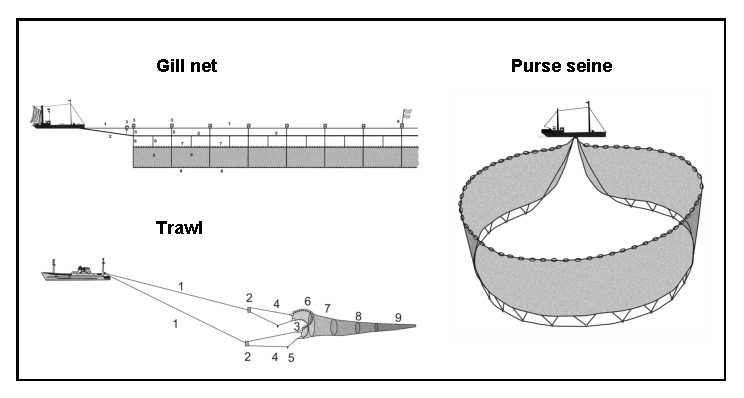
\includegraphics[scale=.42]{fishinggears} 
\caption{Fishing gears commonly used in modern fisheries.\\(Source: Wikimedia commons)}
\label{fig:gears}
\end{figure}

%------------------------------------------------
\section{What is fishing effort?}\index{Fishing effort!Measurement}
\label{section fishing effort}
Fishing effort could be regarded as a commodity produced by varying technologies and in different qualities and quantities. As discussed above, it exists a vast number of different methods of catching fish. Their relative efficiency depends on a number of factors. In general the fishing techniques can be categorised by their influence, action and retention properties in fishing\cite{Chopin1995}.

While some fishing technologies based on concealed nets or traps intend to be invisible for the fish, other technologies aim to attract the fish towards the fishing gear by eye catching and smelling bait. The performance of fishing gears varies depending on fish densities and gear properties. 

There are no obvious ways of measuring fishing effort. Metrics that appear to be useful in some fisheries may be useless in others. In all cases, however, fishing effort is -- as harvest -- measured in various units per unit of time (typically per hour, day, month or year). In a fishery where the fishing fleet is fairly homogeneous, fishing effort may be measured in terms of   
\begin{itemize}
\item Number of vessels per unit of time
\item Number of fishing hours, days or trips per month or year
\item number of working days per time unit
\item Towing hours (for trawl fisheries) per time unit
\item Total numbers of engine horse power units per time unit
\item Total number of hooks (for hand line and long line gears) per time unit
\item Total number of nets (for gill net fleets) per time unit
\item Sum of vessels' length
\item Sum of vessels' tonnage
\end{itemize}
\hfill\break
In the more common cases of heterogeneous fleets, the best way of measuring a standard fishing effort may be to use combinations of the above listed items. Each case must be evaluated individually, based on the specific properties of the fishery in question. A measurement method has high quality if all units are measured by the same scale, also over time.

The difficulty of measuring fishing effort within a given fishery should not be underestimated. Many different units and dimensions could be used to identify single fisheries and the fishing effort of each fishery: Physical properties of the fleet (differences in vessel size, age, engine power, etc.), location (home port), type of operations (composition of different fishing seasons, geographical distribution of fishing grounds, etc.), fishing gears (which may differ between and within seasons), etc.

The fishers need to find profitable combinations of where and when to fish and which gear to use, in order to sustain the fishing activity and maximise their objectives. In principle fisheries management contributes in limiting the area of opportunities, which may encourage the fishing fleet to  specialise in order to be able to more efficiently utilising the available opportunities. 

\begin{definition}[Units to measure fishing effort]
Fishing effort is an input factor in the production of fish harvest. There is no standard unit for the measurement of fishing effort. When using a specific measure for quantifying fishing effort, this measure is assumed a proxy for all other factors constituting the total fishing effort utilised in the production of fish harvest.
\end{definition}

%------------------------------------------------
\section{Production of fishing effort}\index{Fishing effort!Production}\label{fishing effort}

Standard economic production theory assumes non-wasteful and economically efficient production. The interpretation of the latter is discussed in chapter~\ref{chapter 6}. Non-wasteful production represents technological efficiency: Any reduction in input factors will cause reduced production of harvest. In the short run the production technology is given. Production methods and processes (production technology) develops, however, over time and technological breakthroughs could lead to significant shifts in processing technologies. There is good empirical evidence for expecting increased production efficiency over time.

When new technologies develop, they may replace previous technologies or start coexisting with previous technologies. In the production of fishing effort a large range of different technologies have been developed over time, coexisting in many fisheries. From an economic reasoning, we can conclude that each technology has sufficient advantages to survive, because each technology turns out to be more efficient than any other under given conditions. We will later come back to some implications coexistence of different technologies may have.

In general, we assume that fishing effort (\textit{E}) is produced by production processes involving different quantities of labour (\textit{L}) and capital (\textit{K}):
\begin{equation} 
\label{eq:production}
\index{Production functions}
E = E(L,K)
\end{equation}
Usually we expect labour and capital to be substitutes. Hence, the same amount of effort may be produced by different mixes of labour and capital. A given fishing effort could for example be produced by a large quantity of labour and a small quantity of capital, or by a small quantity of labour and a large quantity of capital.

The variables Labour (\textit{L}) and capital (\textit{K}) in Equation~\ref{eq:production} are referred to as \textit{input factors} in the production process. The fishing effort (\textit{E}) is the output of the production process.

Figure~\ref{fig:production} shows three possible shapes Equation~\ref{eq:production} may have for a given quantity $Q$. A curve describing a constant quantity produced by different mixes of input factors while utilising the same technology, is referred to as an \textit{isoquant}. The red and the green isoquants represent two extreme technologies, in between which the sample space of infinitely many possible isoquants representing other technologies, may be found. The red, broken line, illustrates a situation where the input factors labour and capital in fact not are substitutes; increasing one factor does not contribute in increased fishing effort as long as the other factor is not increased. The green isoquant -- the other extremes -- is a straight line, illustrating the case of perfect substitution between the two input factors.

When labour and capital are substitutes the same production is obtained by a small reduction in labour ($-\Delta L$) and a corresponding increase in capital ($\Delta K$). The ratio $- \Delta K / \Delta L$ is the slope of the isoquant and we have
\begin{equation*} 
\lim_{\Delta L \to 0} -\frac{\Delta K}{\Delta L} = -\frac{dK}{dL}
\end{equation*}
From Figure~\ref{fig:production}~we see that the value of the ratio $dK/dL$ is constant in the case of the green line, while it varies in the blue curve. In the case of the latter we can see that while labour continues to decrease, each unit of labour needs to be substituted by an increasing amount of capital in order to sustain the production. 
\begin{figure}[ht]
\centering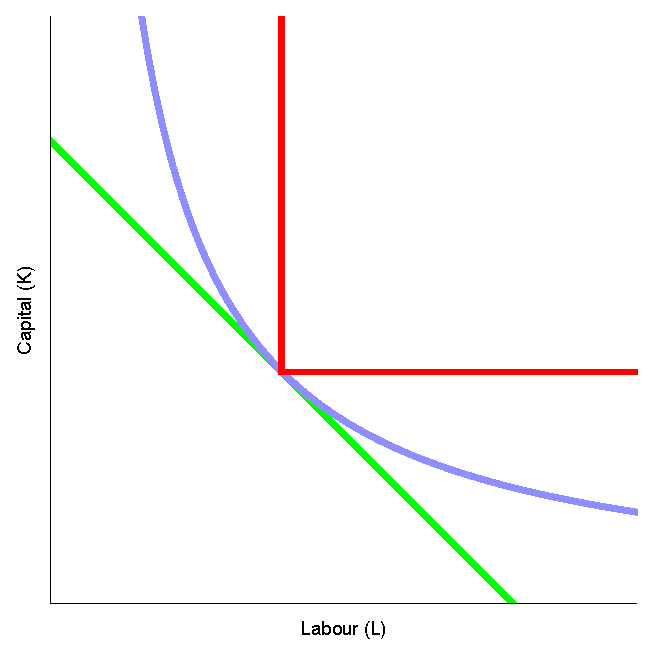
\includegraphics[scale=.7]{fig2}
\caption{Three production processes with different substitution elasticities. The three curves indicates how a constant quantity of fishing effort may be produced by three different production technologies, where the substitution elasticity is zero (red curve), between zero and infinity (blue curve) or infinity (green curve).}
\label{fig:production}
\end{figure}

As discussed in Section~\ref{section fishing effort} fishing effort may be measured in many different ways. The labour involved during a period of time could for example be measured in terms of number of hours all fishers spend on fishing. In that case it may also be relevant to include the time spent on preparing for fishing, for landing the catch, etc. While all input factor (as $L$ and $K$ in Equation~\ref{eq:production}) are measured according to the units that fit each specific factor, all quantities of input factors can be measured in terms of values. The cost of the input of labour and the input of capital are the measurements of the two input factors converted into monetary values by given unit prices of labour and capital. The cost of labour and capital used in the production then constitute the total cost of the produced fishing effort.
%------------------------------------------------
\section{Introduction to elasticities}\index{Elasticity}\label{elast}

Economic theory often makes use of different marginal measures - average values, derivatives and elasticities - all of them reflecting per unit evaluations. For a function $f(x)$, different per unit evaluations could be made
\begin{itemize}
\item the average value of $f(x)$ is $f(x) / x$
\item the marginal value (the derivative with respect to the variable $x$) is expressed by $f'(x) = df(x)/dx$
\item the percentage change in value by a one percent change of the variable (the elasticity with respect to the variable $x$) $f'(x) / (f(x)/x)$
\end{itemize}
\hfill\break
As seen from this listing the elasticity is the ratio between the two other, the derivative divided by the average value. As a ratio the elasticity is unit less, which in particular is an advantage when $f(x)$ can be measured in different units.

An elasticity is a unit-less marginal value that could be regarded as a normalised derivative value. If we look back at the discussion of the slopes of the isoquants in Figure~\ref{fig:production} above, the corresponding elasticity (the elasticity of capital use with respect of use of labour) of the curves is
\begin{equation*} 
\lim_{\Delta L \to 0} -\frac{\frac{\Delta K}{K}}{\frac{\Delta L}{L}} = -\frac{\frac{dK}{K}}{\frac{dL}{L}} = - \frac{dK}{dL} \cdot \frac{L}{K}
\end{equation*}
This elasticity gives the percentage change in capital in order to produce the same quantity after a one percent change in the input of labour. The elasticity (as the slopes of the isoquants) has to be negative since a reduction in use of labour has to be followed by an increase in labour, as a positive shift in labour use has to be compensated by reduced use of capital. As seen from the equation above the elasticity at varying valid combinations of labour and capital will change due changes in the $L/K$-ratio even when the derivative ($dK/dL$) is constant.

In the caption text of Figure~\ref{fig:production} a reference is made to the elasticity of substitution. This is an elasticity often referred to in production economics. This elasticity also involves the prices of the input factors, which will be discussed later.

Above we have introduced three different per unit measures. Why do we need three different methods of unit measurement? In principle one could claim hat there are only two different principles (average and marginal values), since the third measure (elasticity) combines the two others. The two principles are per unit measures but are quite different from each other. While an average value takes into account all unit values, the marginal value only reflects the additional value by the considered unit. In Code box~\ref{code:distancespeed} these differences are illustrated by a simple example.

%\begin{theorem}[Without derivatives the tortoise beats Achilles!]
%\hfill \break
%Zeno of Elea (c. 490 -- c. 430 BC) is credited the famous paradox of race competition between the tortoise and the great Greek hero Achilles. The paradox is embedded in a seemingly perfectly rational story. The tortoise challenges Achilles -- the fastest runner in the world -- to a race. Acknowledging that Achilles is the fastest runner, the tortoise makes a fair suggestion; that Achilles gives him a small head start. Achilles is certain about the victory and does not hesitate in accepting this. The tortoise then claims he will win the race and base this on the following reasoning:
%\\\\
%Suppose the tortoise gets a head start of ten meter. Even though Achilles is a fast runner he will use some time to reach the starting point of the tortoise. And even though the tortoise is slowly moving, he will have moved a short distance during the same period. If we freeze the moment at which Achilles reach the stating point of the tortoise we have a situation similar to the initial situation: The tortoise has a head start of Achilles. Therefore we can repeat the reasoning above, only to find that when Achilles now reaches the new starting point of the tortoise, the tortoise has moved a little further. Achilles can never beat the tortoise.
%\\\\
%The arguments convinced Achilles and he saw no reason to perform the race. The tortoise won without running, but only because Achilles did not know about derivatives. Let us see how far we get without this knowledge:
%\\\\
%Assume that Achilles runs $x$ times faster than the tortoise (obviously $x > 1$) and that the tortoise gets a head start of $h$ meter ($h > 0$). Then the distances covered at the starting point is $0$ meter for Achilles and $h$ meter for the tortoise. When Achilles reaches a distance of $h$ meter the tortoise has moved to $h (1 + 1/x)$ meter, assuming both Achilles and the tortoise to run at a constant speed. This gives the new starting points of Achilles and the tortoise to be respectively $h$ and $h (1 + 1/x)$ meters from the initial starting point. Similarly we may always calculate the new distances after Achilles has reached the tortoises starting point. In general we have: 
%\index{\texttt{NestList}}
%\begin{mmaCell}[index=1]{Input}
%  nextafter[pos_, x_] := 
%    \{pos[[2]], pos[[1]] + (pos[[2]] - pos[[1]])*(1 + 1/x)\}
%\end{mmaCell}
%which gives the expected answer:
%\begin{mmaCell}{Code}
%  nextafter[{0, h}, x]
%\end{mmaCell}
%\begin{mmaCell}{Output}
%  \Big\{h, h \bigg(1 + \mmaFrac{1}{x}\bigg)\Big\}
%\end{mmaCell}
%We can make a nested list:
%\begin{mmaCell}{Code}
%  NestList[nextafter[#, x]&, {0, h}, 2]
%\end{mmaCell}
%\begin{mmaCell}{Output}
%  \Big\{\Big\{0, h\Big\}, \Big\{h, h \bigg(1 + \mmaFrac{1}{x}\bigg)\Big\},
%  \Big\{h \bigg(1 + \mmaFrac{1}{x}\bigg), h + \bigg(-h + h \bigg(1 + \mmaFrac{1}{x}\bigg)\bigg) \bigg(1 + \mmaFrac{1}{x}\bigg)\Big\}\Big\}
%\end{mmaCell}
%Now let us check the results of some numerical values, assume $h = 50$ and $x = 5$ (e.g. that Achilles is five times faster than the tortoise) for the following next six situations:
%\begin{mmaCell}{Code}
%  distances = NestList[nextafter[#, 5]&, {0, 50}, 6]
%\end{mmaCell}
%\begin{mmaCell}{Output}
%  \Big\{\{0, 50\}, \{50, 60\}, \{60, 62\}, \Big\{62, \mmaFrac{312}{5}\Big\}, \Big\{\mmaFrac{312}{5}, \mmaFrac{1562}{25}\Big\},
%  \Big\{\mmaFrac{1562}{25}, \mmaFrac{7812}{125}\Big\}, \Big\{\mmaFrac{7812}{125}, \mmaFrac{39062}{625}\Big\}\Big\}
%\end{mmaCell}
%The numerical values are
%\index{\texttt{N} (Numeric)}
%\begin{mmaCell}{Code}
%  N[distances]
%\end{mmaCell}
%\begin{mmaCell}{Output}
%  \{\{0., 50.\}, \{50., 60.\}, \{60., 62.\}, \{62., 62.4\}, \{62.4, 62.48\}, 
%  \{62.48, 62.496\}, \{62.496, 62.4992\}\}
%\end{mmaCell}
%If we plot the distances obtained after the seven steps we see that Achilles is getting closer and closer to the tortoise. But we do not see Achilles passing the tortoise. What do we miss in %the reasoning above?
%\index{\texttt{Transpose}} \index{\texttt{ListLinePlot}}
%\begin{mmaCell}{Code}
%  ListLinePlot[
%    Transpose[distances], 
%    PlotLegends -> {"Achilles", "Tortoise"}
%  ]
%\end{mmaCell}
%\begin{mmaCell}[moregraphics={moreig={scale=.9}}]{Output}
%  \mmaGraphics{race}
%\end{mmaCell}
%The distances between Achilles and the tortoise in the seven situations above are:
%\index{\texttt{Differences}}
%\begin{mmaCell}{Code}
%  Differences /@ distances
%\end{mmaCell}
%\begin{mmaCell}{Output}
%  \Big\{\{50\}, \{10\}, \{2\}, \Big\{\mmaFrac{2}{5}\Big\}, \Big\{\mmaFrac{2}{25}\Big\}, \Big\{\mmaFrac{2}{125}\Big\}, \Big\{\mmaFrac{2}{625}\Big\}\Big\}
%\end{mmaCell}
%The difference is simply expressed by $h/x^p$ when $t$ is the period number, numbering all the repeated new starts when Achilles reached the previous starting point of the tortoise. The initial starting period is when $p = 0$. Therefore we have:
%\index{\texttt{Range}}
%\begin{mmaCell}{Code}
%  50/5^# & /@ Range[0, 6]
%\end{mmaCell}
%\begin{mmaCell}{Output}
%  \Big\{50, 10, 2, \mmaFrac{2}{5}, \mmaFrac{2}{25}, \mmaFrac{2}{125}, \mmaFrac{2}{625}\Big\}
%\end{mmaCell}
%It is easy to prove that the difference approaches zero as $p$ approaches infinity:
%\index{\texttt{Limit}}
%\begin{mmaCell}{Code}
%  Limit[50/5^p, p -> Infinity]
%\end{mmaCell}
%\begin{mmaCell}{Output}
%  0
%\end{mmaCell}
%Based on this reasoning the tortoise seems to be right! But we all understand it can not be true. Well, there is nothing wrong about the reasoning. We need to remember that $p$ does not represent time but the number of the infinite discrete periods where the starting is repeated. Each of these periods goes faster and faster, as the distance between Achilles and the tortoise approaches zero also the period length approaches zero time units.
%\\\\
%Let us investigate the alternative approach to the problem: The distance ($S_A$) between Achilles and initial starting point is a function of time ($t$). Velocity is a measure we express by the time derivative of the distance: $V_A = dS_A/dt$. Similarly the velocity of the tortoise ($V_T$) is the time derivative of the distance described by the tortoise ($S_T$): $V_T = dS_T/dt$. The distance described by Achilles at time $T$ is found by integrating the velocity of Achilles:
%\begin{equation*} 
%S_A(T) = \int\limits_{t=0}^T V_A \cdot dt = V_A \cdot T
%\end{equation*}
%Correspondingly the distance described by the tortoise at time $T$ is (while including the head start distance $h$):
%\begin{equation*} 
%S_T(T) = h + \int\limits_{t=0}^T V_T \cdot dt = h + V_T \cdot T
%\end{equation*}
%Remember that Achilles runs $x$ times faster than the tortoise; hence, $V_A = x \cdot V_T$. Inserting in the expression fro $S_A(T)$ we get $S_A(T) = x \cdot V_T \cdot T$. Then it is easy to find at which distance Achilles reaches -- and passes (!) -- the tortoise; when $S_A = S_T$. This happens at time $T^*$:
%\begin{align*} 
%S_A &= S_T \\ 
%x \cdot V_T \cdot T^* &= h + V_T \cdot T^* \\
%T^* &= \frac{h}{(x-1) V_T}
%\end{align*}
%Let the corresponding distance be $S^*$. This is found by inserting $T^*$ into the $S_A$ expression
%\begin{align*} 
%S^* &= x \cdot V_T \cdot T^* \\ 
%S^* &= \frac{x}{x-1} \cdot h
%\end{align*}
%In our case, when $h = 50$ and $x = 5$ we get $S^* = 125/2$, independent of velocities (as long as Achilles is five times faster than the tortoise). We see that the numerical value for the distance at which Achilles passes the tortoise is close to the one obtained after the seven discrete steps above, $62.5$. What will the answer be if Achilles only is twice as fast as the tortoise?
%\label{code:derivation}
%\end{theorem}

%\newpage
\begin{theorem}[Per unit calculation - the example of distance and speed]
\hfill \break
Assume that a person goes for a walk. The walk takes one hour and the person shift between two speeds, \texttt{sp1} and \texttt{sp2}. \texttt{sp1} and \texttt{sp2} are measured in units of kilometre per hour (km/h). The first fifteen minutes the person walks at speed \texttt{sp1}, then speed \texttt{sp2} for another half an hour, thereafter speed \texttt{sp1} for another fifteen minutes. We can calculate the walked distance by multiplying the constant speed with the time spent. The total distance can be expressed as a piecewise function:\index{\texttt{Piecewise}}
\begin{mmaCell}[index=1]{Input}
  distance[x_] := Piecewise[\{
  \{sp1 x, x <= 1/4\}, 
  \{sp1*1/4 + sp2 (x - 1/4), 1/4 < x <= 3/4\}, 
  \{sp1*1/4 + sp2 2/4 + sp1*(x - 3/4), x > 3/4\}\}]
\end{mmaCell}
Assume $\texttt{sp1} = 3$ and $\texttt{sp2} = 7$. When walking with a speed of 3 km/h in thirty minutes, the walked distance should be 1.5 km. Another thirty minutes of walk with a speed of 7 km/h adds 3.5 km, 5 km altogether.
\begin{mmaCell}[index=2]{Code}
  distance[1]
\end{mmaCell}
\begin{mmaCell}{Output}
  5
\end{mmaCell}
\index{\texttt{Plot}}
\begin{mmaCell}[index=3]{Code}
  Plot[
    distance[x], {x, 0, 1}, 
    GridLines -> {{1/4, 3/4}, None},
    AxesLabel -> {"Time (hour)", "Distance (km)"}
  ]
\end{mmaCell}
\begin{mmaCell}[moregraphics={moreig={scale=.7}}]{Output}
  \mmaGraphics{walk1}
\end{mmaCell}
Now let us investigate the per unit measures in the following graphical presentation:
\begin{mmaCell}[index=4]{Code}
  Plot[
    {g[x]/x, g'[x], g'[x]/(g[x]/x)}, {x, 0, 1}, 
    PlotRange   -> {0, Automatic}, 
    GridLines   -> {{1/4, 3/4}, None}, 
    AxesLabel   -> {"Time (hour)", "Per unit measure"},
    PlotLegends -> 
      Placed[{"Average", "Marginal", "Elasticity"}, Below],
  ]
\end{mmaCell}
\begin{mmaCell}[moregraphics={moreig={scale=.9}}]{Output}
  \mmaGraphics{walk2}
\end{mmaCell}
We recognise the speeds \texttt{sp1} and \texttt{sp2} as the yellow line segments. These are the marginal values, or the time derivatives of distance. The first quarter the average speed (blue curve) is identical to the marginal value (since the speed is constant). When the speed increases after 15 minutes, the average value increases towards the marginal value before declining the last quarter when the speed drops back to 3 km/h.

The elasticity combines the other two, hence it measures both the immediate change (measured by the marginal value) and the total time and distance. When normalising the marginal value by total values the elasticity measures percentage change in distance by one percent increase in time. The first quarter the percentage change was constant. After increasing the speed also the percentage change in distance by one percent increase in time also increased, even though the speed was constant. The impact from the first quarter brought however the elasticity upwards but as the first quarter makes up a diminishing part of the total, the elasticity falls towards one percent (as the average value gets closer to the marginal). The last change in speed (after 45 minutes) brings the elasticity below one, slightly climbing.
\label{code:distancespeed}
\end{theorem}

\begin{definition}[What is an elasticity?]
\hfill\break
The elasticity of $f(x)$ equals the percentage change in $f(x)$ when $x$ is changed by 1\%
\end{definition}

\begin{figure*}[!htb]
\begin{remark}
\rule{\linewidth}{.1pt}
\floatbox[{\capbeside \thisfloatsetup{capbesideposition={right,top},capbesidewidth=11.8cm}}]{figure}[\FBwidth]
{\caption*{\footnotesize{Here is a Mathematica demonstration presenting \\ graphically the race between \\ Achilles and the tortoise.

\href{http://demonstrations.wolfram.com/ZenosParadoxAchillesAndTheTortoise/}{\\ http://demonstrations.wolfram.com/ \\  ZenosParadoxAchillesAndTheTortoise/}}}}
{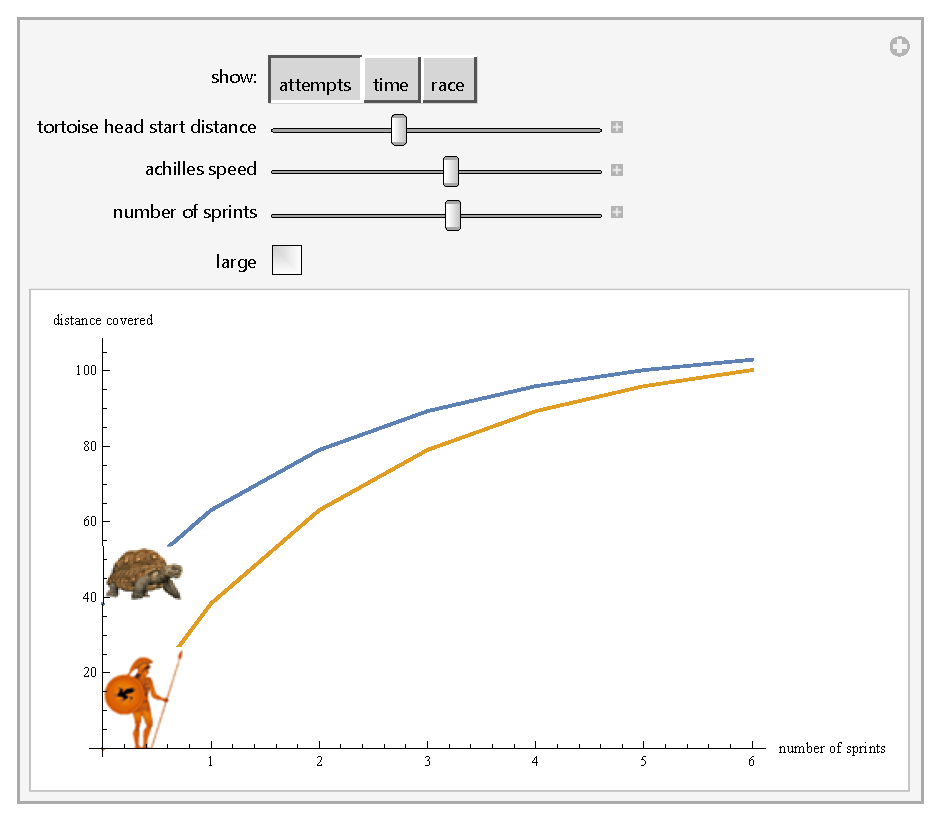
\includegraphics[width=2.8cm]{achilles}}\\
\rule[8pt]{\linewidth}{.1pt}
\end{remark}
\end{figure*}

%------------------------------------------------
\section{The Cobb-Douglas function}\index{Production functions!Cobb-Douglas}

Equation~\ref{eq:production} may have different mathematical expressions depending on the properties of the production processes. The Cobb-Douglas function is often used to describe a production process, assuming \textbf{unit elasticity of substitution} and an \textbf{elasticity of scale} equal 1. We will return to these expression later, after first introducing the Cobb-Douglas production function.

A standard expression of the production of fishing effort ($E$) as a function of labour ($L$) and capital ($K$) as a Cobb-Douglas production process is given by
\begin{equation} 
\label{eq:cobbdouglas}
E(L,K) = A \cdot L^{\alpha} \cdot K^{1-\alpha}
\end{equation}
where $A$ and $\alpha$ are non-negative constants, and $0 \leq \alpha \leq 1$. The \textit{Mathematica} implementation of equation~\ref{eq:cobbdouglas} is given by \texttt{In[1]}\footnote{\textit{Mathematica} inputs are numbered in this way. Corresponding numbering of output is \texttt{Out[1]}.} in Code box~\ref{code:cobbdouglas} below where also the output elasticities of the two input factors are expressed.
\begin{theorem}[Output elasticities in the Cobb-Douglas function]\index{Elasticity!of output}
\hfill \break
Defining the Cobb-Douglas function in \textit{Mathematica}:\footnote{Since all internal \textit{Mathematica} commands start with a capital letter we prefer to use lower case letters in our variables, to avoid confusion. In this code the fishing effort symbol ($E$) in equation~\ref{eq:cobbdouglas} is replaced by $cd$, indicating that it is a Cobb-Douglas equation.}
\begin{mmaCell}[index=1]{Input}
  cd[l_, k_] := A * l^\(\pmb{\alpha}\) * k^(1 - \(\pmb{\alpha}\))
\end{mmaCell}
Now find the output elasticity with respect of labour (\texttt{l}):
\index{\texttt{D} (Derivative)}
\begin{mmaCell}[index=2]{Code}
  D[cd[l, k], l] * l / cd[l, k]
\end{mmaCell}
\begin{mmaCell}{Output}
  \(\pmb{\alpha}\)
\end{mmaCell}
and the output elasticity with respect of capital (\texttt{k}):
\begin{mmaCell}[index=3]{Code}
  D[cd[l, k], k] * k / cd[l, k]
\end{mmaCell}
\begin{mmaCell}{Output}
  1 - \(\pmb{\alpha}\)
\end{mmaCell}
\label{code:cobbdouglas}
\end{theorem}

Capital cost consists of two main components: 1) The market value of the fishing gears and other materials used in the fishing operation (\textit{c}), and 2) the value of the forgone benefits by spending the capital on materials for fishing ($c_o$) and not elsewhere. The latter is often referred to as \textit{the opportunity cost} of capital.

The cost of labour could be calculated in different ways. If the labour is hired, the labour cost is the wages paid ($w$) and the opportunity cost of the capital spend on labour ($l_o$). For an independent fisher, spending the time on fishing, the labour cost is the forgone income by utilising the labour achievement in the best alternative placement ($c_o$).

The three fishing technologies mentioned above (angling, long line and hand line fishing) use different mixes of labour and capital in their production of fishing effort.
%------------------------------------------------
\section{The CES function}\index{Production functions!CES} \label{cesf}

The CES function provides a more general formulation of equation~\ref{eq:production}. The abbreviation CES means \textit{Constant Elasticity of Substitution} and figure~\ref{fig:production} shows the two extremes of an infinitely large elasticity of substitution (green) and zero elasticity of substitution (red).

The Cobb-Douglas function is a special case of the CES function, with a constant elasticity of substitution equal one (unit elasticity of substitution). The blue curve in figure~\ref{fig:production} shows a Cobb-Douglas curve, while all three curves are special cases of a CES function.
\begin{theorem}[Output elasticities in the CES function]\label{code:ceselasticities}
\hfill \break
Defining the CES function in \textit{Mathematica}:
\begin{mmaCell}[index=1,
  morepattern={l,k,l_,k_},
  moredefined={\(\pmb{\alpha}\),r}
]{Input}
  ces[l_, k_] := (\(\pmb{\alpha}\) l^r + (1 - \(\pmb{\alpha}\)) k^r)^(1/r)
\end{mmaCell}
where $r$ is a parameter related to the elasticity of substitution. The elasticity of substitution is $\eta = 1/(1-r)$. Now, find the output elasticity with respect of labour ($l$):
\index{\texttt{D} (Derivative)}
\begin{mmaCell}[morepattern={l,k,l_,k_}]{Code}
  D[ces[l, k], l] * l / ces[l, k]
\end{mmaCell}
\begin{mmaCell}{Output}
  \mmaFrac{\mmaSup{l}{r} \(\pmb{\alpha}\)}{\mmaSup{k}{r} (1-\(\pmb{\alpha}\)) + \mmaSup{l}{r} \(\pmb{\alpha}\)}
\end{mmaCell}
and the output elasticity with respect of capital ($k$):
\begin{mmaCell}[index=3]{Code}
  D[ces[l, k], k] * k / ces[l, k]
\end{mmaCell}
\begin{mmaCell}{Output}
  \mmaFrac{\mmaSup{k}{r} (1-\(\pmb{\alpha}\))}{\mmaSup{k}{r} (1-\(\pmb{\alpha}\)) + \mmaSup{l}{r} \(\pmb{\alpha}\)}
\end{mmaCell}
\index{Elasticity!of substitution}Let us make 3D plots of the three cases indicated in figure~\ref{fig:production}, when the elasticity of substitution ($\eta$) equals $\infty$, 1 and 0 respectively. In the plots the input factors, labour and capital, are represented by the two horizontal axes while the output is measured upwards.

For $\eta = \infty$ (perfect elasticity of substitution):
\index{\texttt{Transpose}}\index{\texttt{Range}}\index{\texttt{Plot3D}}
\begin{mmaCell}{Input}
  Plot3D[
    ces[l, k] /. \{r -> 1, \(\pmb{\alpha}\) -> 1/2\}, 
    \{k, 0, 1\}, \{l, 0, 1\},
    MeshFunctions -> \{#3&\}, 
    Mesh -> \{Transpose[
      \{Range[5]/6,\{#,#,Directive[Thickness[.02], Green],#,#\}\}
    ] & @ Black\}
  ]
\end{mmaCell}
\begin{mmaCell}[moregraphics={moreig={scale=.4}}]{Output}
  \mmaGraphics{ces1}
\end{mmaCell}
For $\eta = 1$ (the Cobb-Douglas function):
\index{\texttt{Limit}}\index{\texttt{Plot3D}}\index{\texttt{Transpose}}\index{\texttt{Range}}
\begin{mmaCell}{Input}
  Plot3D[
    Evaluate@Limit[ces[l, k]/.\{\(\pmb{\alpha}\) -> 1/2\},\{r -> 0\}],
    \{k, 0, 1\}, \{l, 0, 1\},
    MeshFunctions -> \{#3&\}, 
    Mesh -> \{Transpose[
      \{Range[5]/6, 
      \{#,#,Directive[Thickness[.02],Lighter@Lighter@Blue],#,#\}\}
    ] & @ Black\}
  ]
\end{mmaCell}
\begin{mmaCell}[moregraphics={moreig={scale=.4}}]{Output}
  \mmaGraphics{ces2}
\end{mmaCell}
For $\eta \approx 0$ (the Leontief function):\index{\texttt{Plot3D}}\index{\texttt{Transpose}}\index{\texttt{Range}}
\begin{mmaCell}{Input}
  Plot3D[
    ces[l, k]/.\{r->-1000000000000, \(\pmb{\alpha}\)->1/2\}, 
    \{k, 0, 1\}, \{l, 0, 1\},
    MeshFunctions -> \{#3&\}, 
    Mesh -> \{Transpose[
      \{Range[5]/6,\{#,#,Directive[Thickness[.02], Red],#,#\}\}
    ] & @ Black\}
  ]
\end{mmaCell}
\begin{mmaCell}[moregraphics={moreig={scale=.4}}]{Output}
  \mmaGraphics{ces3}
\end{mmaCell}
In each of the three plots above a constant value of output is indicated by colour according to the colours used in figure~\ref{fig:production}, green ($\eta = \infty$), blue ($\eta = 1$) and red ($\eta = 0$).
\label{code:ces}
\end{theorem}
%------------------------------------------------
\section{Elasticity of scale}\index{Elasticity!of scale}\label{elasticityofscale}

The principle of elasticises is presented in section~\ref{elast} and output elasticities are found for the Cobb-Douglas function (Code box~\ref{code:cobbdouglas}) and the CES function (Code box~\ref{code:ces}). The interpretations of the output elasticities are straightforward: When one of the input factors, $l$ or $k$, changes (increases or decreases) by one percent, the production output is changed accordingly by a percentage equal to the output elasticity of the input factor.

\begin{theorem}[Continues from code box~\ref{code:ces}]
\hfill \break
Also for the case of the CES function the elasticity of scale equals one in this case. Here it is convenient to employ \textit{Mathematica} to find the solution:
\index{\texttt{D} (Derivative)}\index{\texttt{Simplify}}
\begin{mmaCell}[index=7,morepattern={l,k,l_,k_}]{Input}
  Simplify[D[ces[l,k],l]*l/ces[l,k] + D[ces[l,k],k]*k/ces[l,k]]
\end{mmaCell}
\begin{mmaCell}{Output}
  1
\end{mmaCell}
\end{theorem}

According to the results in Code box~\ref{code:cobbdouglas} the output elasticity of labour in the Cobb-Douglas function is $\alpha$ and the output elasticity of capital is $1 - \alpha$. If both input factors are changed simultaneously by one percent, the total change of output equals the sum of the two output elasticities. For the Cobb-Douglas equation it is easy to see that $\alpha + (1 - \alpha) = 1$. This sum is usually referred to as the elasticity of scale (or returns to scale), indicating the effect up- and down-scaling have on the produced quantity. 

The elasticity of scale is usually assumed to equal one, indicating that there are no economics of scale in the production. This represents a normal production but needs not to always be the case. Both the Cobb-Douglas function and the CES function may be adjusted to accommodate scale elasticities different from one. A simple and general formulation of the first function is
\begin{equation} 
\label{eq:cobbdouglas2}
E(L,K) = A \cdot L^{\alpha} \cdot K^{\beta}
\end{equation}
where the elasticity of scale is $\epsilon = \alpha + \beta$. If the two input factors ($L$ and $K$) are both increased/decreased by one percent, the total effort production ($E$) increases/decreases by $\epsilon$ percent.The contribution from the increase or decrease of labour ($L$) is $\alpha$ and the contribution from capital ($K$) is $\beta$ percent.

In some productions we find that $\epsilon > 1$, providing increasing return to scale, meaning that when scaling up the production it becomes relatively more efficient. Depending on market factors this may lead to economics of scale, giving an advantage to the large producers compared with smalls.

%------------------------------------------------
\section*{Exercises}\index{Exercises!Chapter 2}
\addcontentsline{toc}{section}{Exercises}

\begin{exercise}
Assume a production of fishing effort according to equation~\ref{eq:cobbdouglas2} where $\alpha = 1$ and $\beta = 1.5$. Let labour ($L$) and capital ($K$) increase with 10\%. How much will the production of fishing effort increase?
\end{exercise}

\begin{exercise}
In the CES-function in code box~\ref{code:ceselasticities} assume $\eta = 1$. Find the output elasticities of labour and capital.
\end{exercise}

%\begin{figure}[!htb]
%\minipage{0.32\textwidth}
%  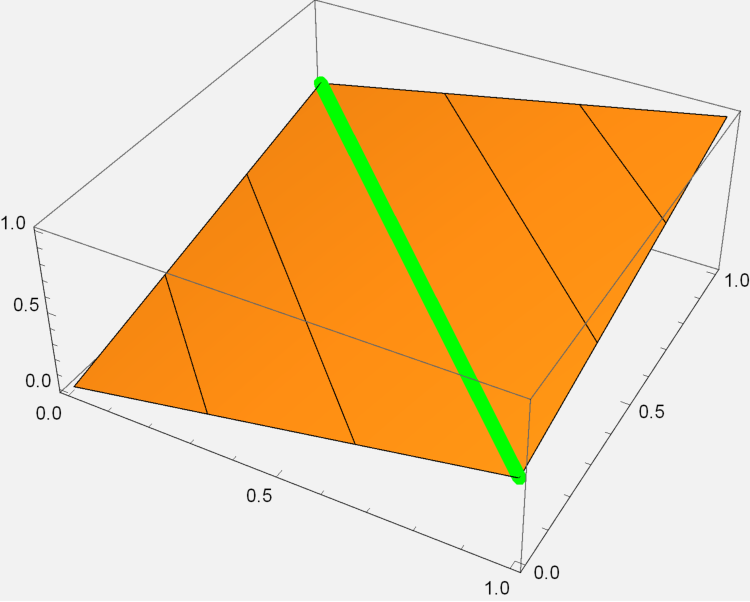
\includegraphics[width=\linewidth]{ces1.pdf}
%  \caption{\(\eta\) = \(\infty\)}\label{fig:awesome_image1}
%\endminipage\hfill
%\minipage{0.32\textwidth}
%  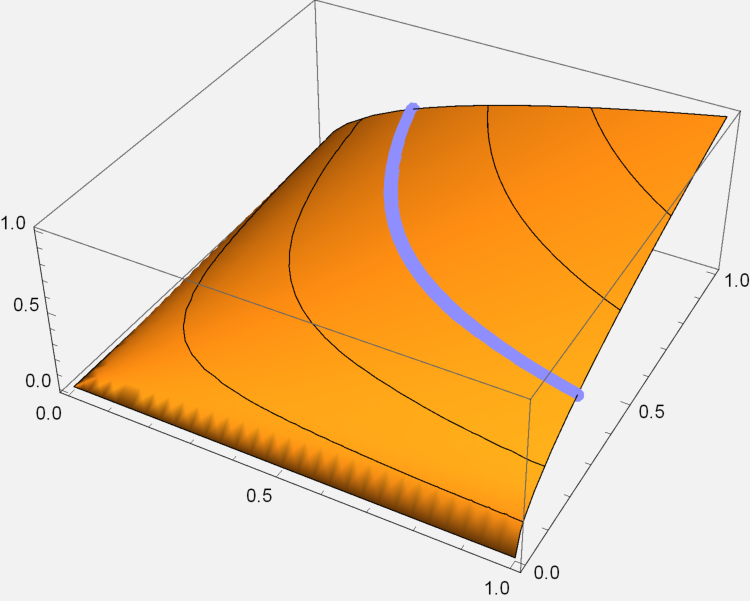
\includegraphics[width=\linewidth]{ces2.pdf}
%  \caption{\(\eta\) = 1}\label{fig:awesome_image2}
%\endminipage\hfill
%\minipage{0.32\textwidth}%
%  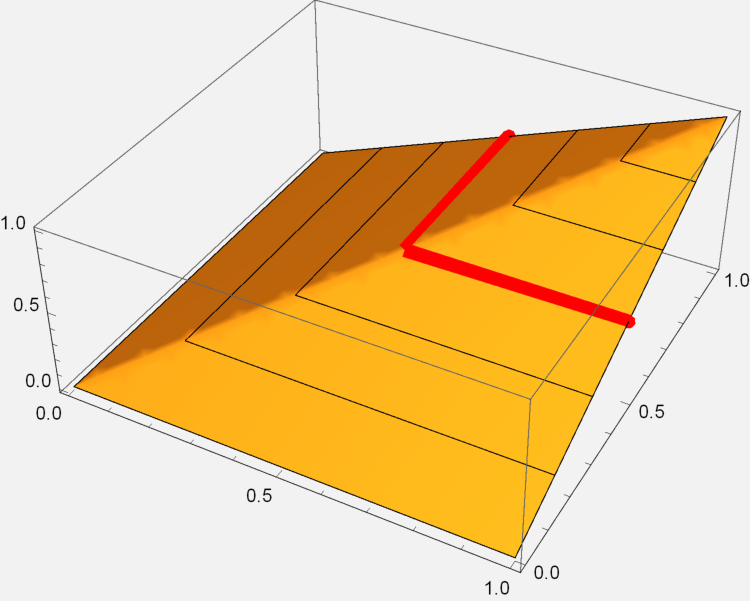
\includegraphics[width=\linewidth]{ces3.pdf}
%  \caption{\(\eta\) = 0}\label{fig:awesome_image3}
%\endminipage
%\end{figure}

%------------------------------------------------


\chapterimage{h3.jpg} % Chapter heading image

\chapter{Fish catch production} \label{chapter 3}
%----------------------------------------------------------------------------------------
%	CHAPTER 3
%----------------------------------------------------------------------------------------

\section{Catch production}\index{Catch production}

In section~\ref{requirements} necessary requirements of producing fishing effort were discussed. It is however not sufficient to know how to catch fish, fish stock resources also need to be available for catch. In economic terms we would say that the fish stock is an essential input factor in the production of catch. The other essential factor in the production of catch is the fishers' fishing aptitude which in the following referred to as the fishing effort.

Catch production is a production process following the principle of technological efficient production discussed in chapter~\ref{chapter 2} where some well-known production functions were introduced. In this chapter we will discuss further how to implement the Cobb-Douglas function (equation~\ref{eq:cobbdouglas2}) to describe fish catch production.

In chapter~\ref{chapter 2} we have already discussed how fishing effort ($E$) is produced by the input factors labour ($L$) and capital ($K$). Now we consider a production process where fishing effort as an input factor in the output is fish harvest. Fishing effort alone is not sufficient to produce harvest of fish, it is also necessary to have access to a fish stock resource. Therefore the available fish stock also is an input factor in the production of fish harvest

In chapter~\ref{chapter 5} we will discuss further the properties of the fish stock, here we only consider the fish stock in terms of available biomass as one of the two input factors to produce fish catches.

%------------------------------------------------
\section{Stock assessment based on catch statistics}

Stock assessment is the core foundation of modern fisheries management. Time series of stock assessments provides information about growth potential, variability and possible exploitation levels.

The simplest stock assessment method is to compare the amount of catch per unit of fishing intensity (catch per unit of effort, $CPUE$) between different areas or periods. The highest $CPUE$ is believed to reflect the highest abundance.

This is however not a method to estimate the real number of fish in an area at a point in time but merely a relative measure to rank different observations. However, in order to tell if the fish abundance is increasing or decreasing it is sufficient to measure the relative changes.

The indexes by which we measure relative changes (e.g. $CPUE$) are regarded as stock estimates. In fact, this is the case also for the more sophisticated stock assessment methods utilised in data rich single species fisheries as for example the Northeast Arctic cod fishery. In this fishery there exists high resolution catch data, annual survey data and a number of scientific studies contributing in enriching the stock assessment methodology and tuning processes used to evaluate the state of the stock at any point in time.

Let us move back to the basic observation which we may label the $CPUE$ methodology, where a large catch with a given effort signalise a larger stock abundance than a small catch with the same effort at another point in time. In its most rudimentary form the $CPUE$ methodology assumes a linear catch function:
\begin{equation} 
\label{eq:schaeffer}
H(E,X) = q \cdot E \cdot X
\end{equation}
where $H$ is the harvest produced by the fishing effort, $E$, and the stock abundance (measured in biomass), $X$. $q$ is often referred to as the catchability coefficient, a scaling parameter also reflecting the technological property of the fishing gear in use.

As seen in section~\ref{elasticityofscale} It is easy to see from equation~\ref{eq:schaeffer} that catch per unit of effort ($CPUE$) is linear to the stock index $q \cdot X$:
\begin{equation} 
\label{eq:cpue}
CPUE = H(E,X)/E = q \cdot X
\end{equation}

If we had an accurate estimate of the value of $q$, we could actually determine the stock biomass in nature, $X$. In most cases it is however sufficient to know if the stock is growing or declining to make non-critical management decisions. Then the $CPUE$-measure is sufficient; given that equation~\ref{eq:schaeffer} holds and that we are able to measure catch ($H$) and effort ($E$) correctly. The latter is a major problem which is dealt with other places in this document. Here we will discuss further the methodology, given that accurate catch and effort observations exist.

Measurement of fishing effort in a consistent manner is a challenge which is not easily solved. There are no standard methods of standardising effort in a heterogeneous fleet at a point in time. In addition, fleet efficiency changes (typically increases) over time, creating a systematic error when comparing fishing effort measures in different time periods.

\begin{theorem}[Simple stock assessment by $CPUE$ calculations]\index{Stock assessment!by $CPUE$}
\hfill \break
Assume that we have access to time series of catch data and standardised fishing effort over a period of ten years. The catch time series is:
\begin{mmaCell}[index=1]{Input}
  catch = \{
  2384, 2361, 1586, 1889, 1766, 2456, 1068, 1905, 1425, 1957\};
\end{mmaCell}
The effort was 100 the first year and increased by 10 every year after. The $CPUE$ development over time is seen by plotting catch per effort for each year
\index{\texttt{Table}}\index{\texttt{ListLinePlot}}
\begin{mmaCell}{Input}
  ListLinePlot[
    catch/Table[100 + 10*t, \{t, 0, 9\}], 
    Mesh       -> All,
    Frame      -> True,
    PlotTheme  -> "Detailed",
    FrameLabel -> \{"Year","CPUE"\}
  ]
\end{mmaCell}
\begin{mmaCell}[moregraphics={moreig={scale=.7}}]{Output}
  \mmaGraphics{cpue}
\end{mmaCell}
We observe a down-sloping trend in the $CPUE$ measures and assume a linear model
\index{\texttt{LinearModelFit}}\index{\texttt{Transpose}}\index{\texttt{Table}}
\begin{mmaCell}{Input}
  model1 = LinearModelFit[
  Transpose[\{#, catch/#\} &@Table[100 + 10*i, \{i, 0, 9\}]], x, x]
\end{mmaCell}
\begin{mmaCell}[moregraphics={moreig={scale=1}}]{Output}
  \mmaGraphics{model1}
\end{mmaCell}
We see that about 67.5\% of the variation is explained by the linear model
\begin{mmaCell}{Input}
  model1["RSquared"]
\end{mmaCell}
\begin{mmaCell}{Output}
  0.675255
\end{mmaCell}
and we retrieve the analysis of variance by
\begin{mmaCell}{Input}
  model1["ANOVATable"]
\end{mmaCell}
\begin{mmaCell}[moregraphics={moreig={scale=1}}]{Output}
  \mmaGraphics{anova}
\end{mmaCell}
The results of the linear regression is plotted together with the $CPUE$ observation versus fishing effort.
\index{\texttt{Show}}\index{\texttt{Plot}}\index{\texttt{ListLinePlot}}\index{\texttt{Transpose}}
\begin{mmaCell}{Input}
  Show[\{
    Plot[model1[e], \{e, 0, 240\}, PlotStyle -> Dashed],
    ListLinePlot[
      Transpose[\{#, catch/#\} & @ Table[100 + 10*i, \{i,0,9\}]], 
      Mesh -> All
    ]\}, 
    Frame            -> True, 
    PlotRangePadding -> None,
    PlotRange        -> \{0, All\}, 
    FrameLabel       -> \{"Effort", "CPUE"\}
  ]
\end{mmaCell}
\begin{mmaCell}[moregraphics={moreig={scale=.7}}]{Output}
  \mmaGraphics{cpue2}
\end{mmaCell}
Multiplying the $CPUE$ values above with effort gives the catch and the linear regression now describes a parabolic curve through the origin.
\index{\texttt{Show}}\index{\texttt{Plot}}\index{\texttt{ListLinePlot}}\index{\texttt{Transpose}}
\begin{mmaCell}{Input}
  Show[\{
    Plot[model1[e] * e, \{e, 0, 240\}, PlotStyle -> Dashed],
    ListLinePlot[
      Transpose[\{Table[100 + 10*i, \{i, 0, 9\}], catch\}],
      Mesh -> All
    ]\}, 
    Frame            -> True, 
    PlotRangePadding -> None,
    PlotRange        -> \{0, 2600\}, 
    FrameLabel       -> \{"Effort", "Catch"\}
  ]
\end{mmaCell}
\begin{mmaCell}[moregraphics={moreig={scale=.7}}]{Output}
  \mmaGraphics{catch}
\end{mmaCell}
\label{code:cobbdouglas3}
\end{theorem}

In principle catch quantities are easier to measure than fishing effort. It demands however a system of retrieving such information without hidden, manipulated or illegal catches disturbing the data samples.

\begin{corollary}[How many frogs are needed?]
\hfill \break
\small{Now, having learned the concept of \textit{catch per unit of effort}, you should be able to solve this small puzzle:

If 37 frogs catch 37 flies in 37 minutes, how many frogs is needed to catch 52 flies in 52 minutes?

}
\label{highlight:frogsandflies}
\end{corollary}

%------------------------------------------------
\section{Cobb-Douglas catch production}

Catch is produced by two input factors, fishing effort ($E$) and stock biomass ($X$) as indicated in equation~\ref{eq:schaeffer}. We now assume the more the more general Cobb-Douglas production function expressed in equation~\ref{eq:cobbdouglas2}):
\begin{equation} 
\label{eq:cobbdouglas3}
H(E,X) = q \cdot E^{\alpha} \cdot X^{\beta}
\end{equation}
We see that this expression is equivalent to equation~\ref{eq:schaeffer} when $\alpha = \beta = 1$.

There may be reasons to expect $\alpha = 1$ and $0 < \beta < 1$\cite{Hannesson1983,Eide2003a}. If $E$ is measured in number of homogeneous boats we should expect two boats to fish the double of one boat, given a constant stock size ($X$). Hence, $\alpha$ should equal 1, since $2 \cdot q \cdot E^\alpha \cdot X^\beta = q \cdot (2 \cdot E)^\alpha \cdot X^\beta$ when $\alpha = 1$.

\index{Fishing gears!Gill net}The value of $\beta$ depends both on biological properties of the fish stock in question (typically $\beta$ will be lower for schooling species than for non-schooling species) and the properties of the harvesting technology (gillnetting is for example expected to have higher $\beta$-values than longlining has).

On the basis of similar reasoning as those above, a better approximation -- without adding more parameters -- may be obtained by assuming $\beta = 1/2$:
\begin{equation} 
\label{eq:cobbdouglas4}
H(E,X) = q \cdot E \cdot \sqrt[]{X}
\end{equation}

%------------------------------------------------
\section{Properties of fishing gears}

In chapter~\ref{chapter 2} selected fishing gears are listed. Some gears are fishing randomly fish passing through the area (some traps and gill nets). Other gears aim to attract fish to swim into traps or onto hooks where they are captured (fish pots, long line, hand line, etc.), while other fishing gears actively move towards the fish to capture it (trawl, purse seine, Danish seine, etc.).

Gill nets represent gears which in principle aim to be invisible for the fish and therefore catch fish that randomly pass through the nets. In a sea of uniform distribution and random movement of fish (as illustrated in the two left panels of figure~\ref{fig:gearproperties}) the expected catch of a fishing gear will be constant, independent of where it is placed in the sea. In the case of gill nets the expected catch in the left panel is one quarter of the expected catch in the right panel, because the density of fish (number of black dots) is four times higher in the centre panel than in the left panel. This is expressed in a \textit{stock-output elasticity} of one ($\beta = 1$) in equation~\ref{eq:cobbdouglas3}. 

\begin{figure}[ht]
\centering
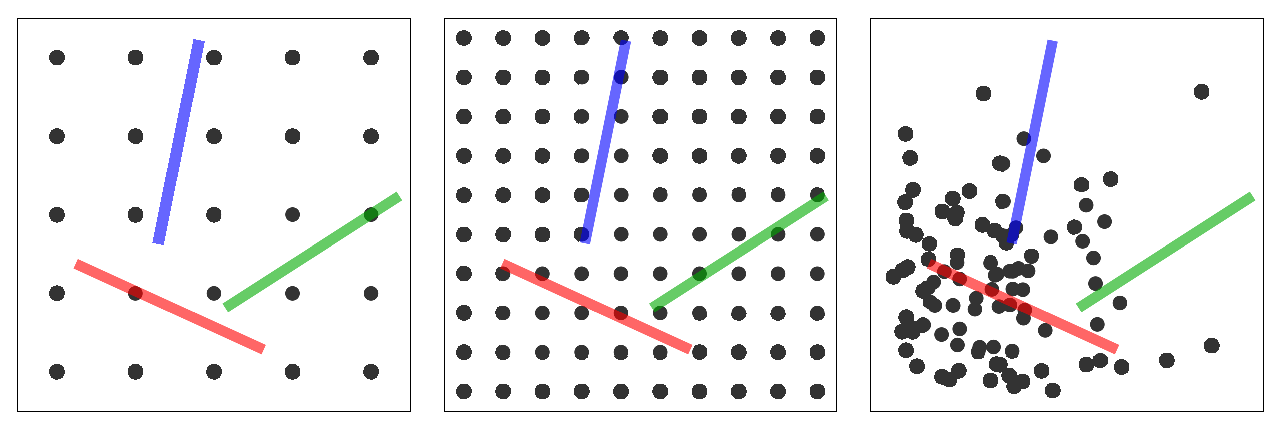
\includegraphics[scale=.7]{gearproperties}
\caption{Three fishing gears (red, blue and green) placed in a sea of uniform fish distribution (black dots) with low (left panel) and high (centre panel) densities of fish, and in a non-uniformly distributed fish stock in the right panel. The number of dots (indicating fishes) is 25 to the left and 100 in the two other panels.}
\label{fig:gearproperties}
\end{figure}


\index{Fishing gears!Gill net}Fishing gears like gill nets or traps have higher stock-output elasticities than other gears and when assuming random movement of fish, $\beta$ will approach one. With a uniform distribution of a fish biomass $X$ and a perfectly invisible gill net (not affecting the fish decisions on where to move), the gill net will catch a fixed proportion per square meter net per unit of time of the stock, depending on the probability the fish has to pass through the net and the per period of time movement per fish. As seen above, the interpretation of this is that $\beta = 1$.

\index{\texttt{PlotTheme}}\index{\texttt{PlotLegends}}\index{\texttt{Plot}}\index{\texttt{Sqrt}}\index{\texttt{PlotRangePadding}}\index{\texttt{FrameLabel}}\index{Fishing gears!Gill net}\index{Fishing gears!Long line}
\begin{theorem}[The most efficient fleet]
\hfill \break
Assume two homogeneous fleets exploiting the same fish stock. The first fleet uses gill nets, the other long line. In both cases the catch per unit of time is described by a Cobb-Douglas function (equation~\ref{eq:cobbdouglas3}) where $\alpha = q = 1$. Unit catch of effort for each fleet group therefore is described by $H(E, X)/E = X^\beta$. We expect that the $\beta$-value of gill nets to be higher than for long line. When assuming uniform distribution and random movement of each fish -- like in the two panels to the left in figure~\ref{fig:gearproperties} -- we set the $\beta$-value of gill nets equal 1 and $1/2$ for long line.
\begin{mmaCell}[index=1]{Input}
  Plot[
    \{x, Sqrt[x]\}, \{x, 0, 2\},
    PlotTheme        -> "Detailed",
    PlotLegends      -> \{"Gill net", "Long line"\},
    PlotRangePadding -> None
    FrameLabel       -> \{"Stock biomass (X)",
                        "Catch per unit of effort"\}
  ]
\end{mmaCell}
\begin{mmaCell}[moregraphics={moreig={scale=.8}}]{Output}
  \mmaGraphics{efficientgear}
\end{mmaCell}
We see that long line catch more per unit of effort when $X < 1$ and gill net catch more when $X > 1$. From the discussion of output-elasticities in the Cobb-Douglas equation (see code box~\ref{code:cobbdouglas}) we know that $\beta$ gives the percentage increase in the catch of a one percent increase in the stock size. Hence, the long line catch increases less than the gill net catch when the stock biomass increases. We can conclude that none of the two fleets are in general more efficient than the other, it all depends on the stock size.
\label{code:costefficient}
\end{theorem}

When these conditions is not met (uniform distribution of fish and invisible fishing gears) typically the $\beta$-value will be less than one. The right hand panel in figure~\ref{fig:gearproperties} displays a situation of non-uniform distribution of fish. Obviously the red gear is expected to fish more than the blue or green gear. 

The distribution of fish may be affected of the gear itself, as when for example using baited hooks (longline or handline). The fish will gather around the baited hook and the density of fish will locally increase. Hence, the chance of hooking one fish becomes higher than indicated by the mean fish density of the area.

Several studies of the Northeast Arctic cod fishery indicate $\beta$-values below 1. The findings of Hannesson (1983)\cite{Hannesson1983} (covering the period 1971–78), Flaaten (1987)\cite{Flaaten1987} and Eide et al. (2003)\cite{Eide2003a} (covering the period 1971–85, as in this study) all suggest $\beta$-values between 0.6-0.9 for gill nets, while all other fishing gears (trawl, danish seine, long line and hand line) have $\beta$-values below 0.5.

Most studies assume a priori $\alpha = 1$ for all gears, expecting catch production to be proportional to fishing effort. This seems to be a reasonable assumption but empirical studies also indicate that the $\alpha$-value may exceed one\cite{Eide2003a}. The interpretation of such findings could be a higher efficiency when many are participating in the fishing. By observing other fishing vessels the fishers get a better knowledge about the distribution of fish and can reduce the time they use to find high densities of fish. But the findings may also simply be a reflection of the fact that the fishing activity increases when the availability is high. In that case the a priori assumption $\alpha = 1$ could be a better suggestion that $\alpha > 1$.

\index{Fishing gears!Gill net}\index{Fishing gears!Long line}Fishing gear properties are however not the only factor affecting the $\beta$-value. Also the spatial distribution of fish has a great impact on the stock-output elasticity ($\beta$). When fishing randomly by an invisible gear (e.g. the ideal gill net) on a uniformly distributed stock biomass $X$, then $\beta = 1$. The opposite is a schooling stock and actively targeting the schools where the density of fish is constant, independent of the size of $X$ (given that $X > 0$). In the idealised case of this $\beta = 0$. In that case equation~\ref{eq:cobbdouglas3}) simplifies to $H(E) = q \cdot E^{\alpha}$, where the produced harvest is independent of the stock size $X$.

The example provided in code box~\ref{code:costefficient} shows how some gears, in this case long line, compensate for reduced density of fish in the exploited area by luring the fish to have a higher density around the fishing gear by allurements like bait. The advantage of a gill net, however, is that since it is invisible and don't use allurements, it may take a grater share when the natural density of fish increases, while the density around a line hook is less dependent of the natural density in the area.

\index{Fishing gears!Conventional}\index{Fishing gears!Active and passive}\begin{corollary}[Conventional gears and trawl]
\hfill \break
Gill net and other invisible traps (without bait) differ from other gears that aim to attract fish. But they also differ from gears that catch fish by moving around. In fact, the production equation of such gears are closer to baited gears than to gill nets and invisible traps. The stock-output elasticity ($\beta$ in equation~\ref{eq:cobbdouglas3}) therefore is well bellow 1 for such gears, while it is closer to 1 for gill nets, given a close to uniform spatial stock distribution. Hence, the stock-output-elasticities of for example trawl and long line are closer to each other that to the stock-output-elasticity of gill net. 

It may therefore be discussed how fruitful the common classification of gears in \textit{conventional gears} (most gears except trawl) and \textit{trawl} is. From the view point of production properties it may be better to differ between \textit{active gears} (moving the gear or aiming to move the fish) and \textit{passive gears} (gears fishing randomly what is passing by).
\end{corollary}

\begin{figure}[!htb]
\begin{remark}
\rule{\linewidth}{.1pt}
\floatbox[{\capbeside\thisfloatsetup{capbesideposition={right,top},capbesidewidth=11.8cm}}]{figure}[\FBwidth]
{\caption*{\footnotesize{Study fishing gear properties under \\different densities and distributions of fish::

\href{http://demonstrations.wolfram.com/FishingWithLongLineOrGillNet/}{\\ http://demonstrations.wolfram.com/FishingWithLongLineOrGillNet/ \\ }}}}
{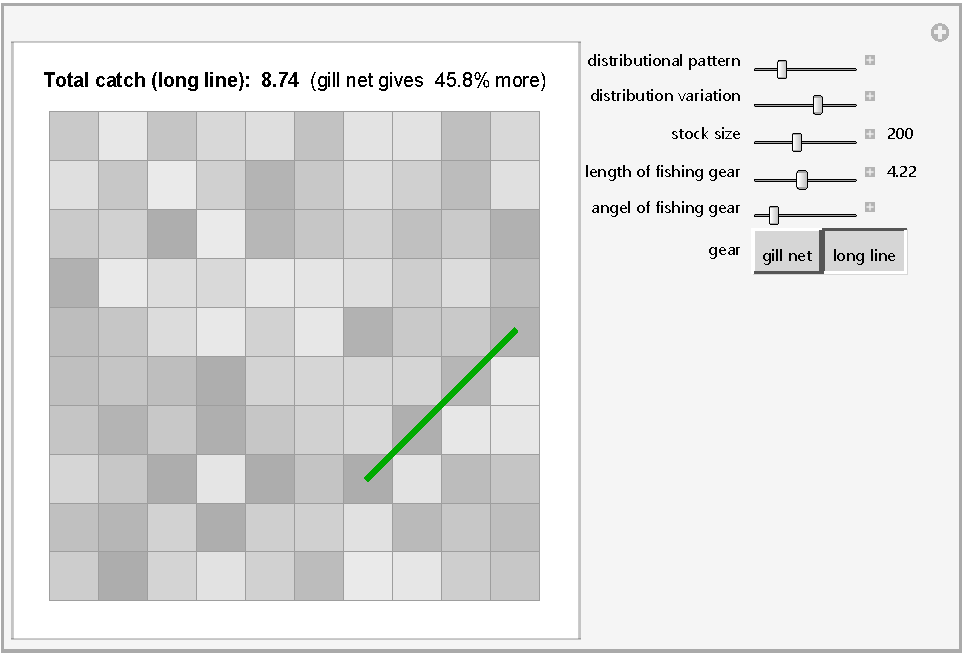
\includegraphics[width=2.8cm]{demo_fishing_gear}}\\
\rule[10pt]{\linewidth}{.1pt}\end{remark}\end{figure}

%------------------------------------------------
\section{Gear selection}
While $\beta$ expresses the relation between fish densities and catch, the selective capacities of fishing gears are not captured by this parameter. Different fishing gears have different properties of retaining fish of different sizes. The construction and layout of fishing gears may change the selecting properties, which makes gear selection into an important management tool. Gear regulations are among the oldest regulatory means in fishing.

\begin{figure}[ht]
\centering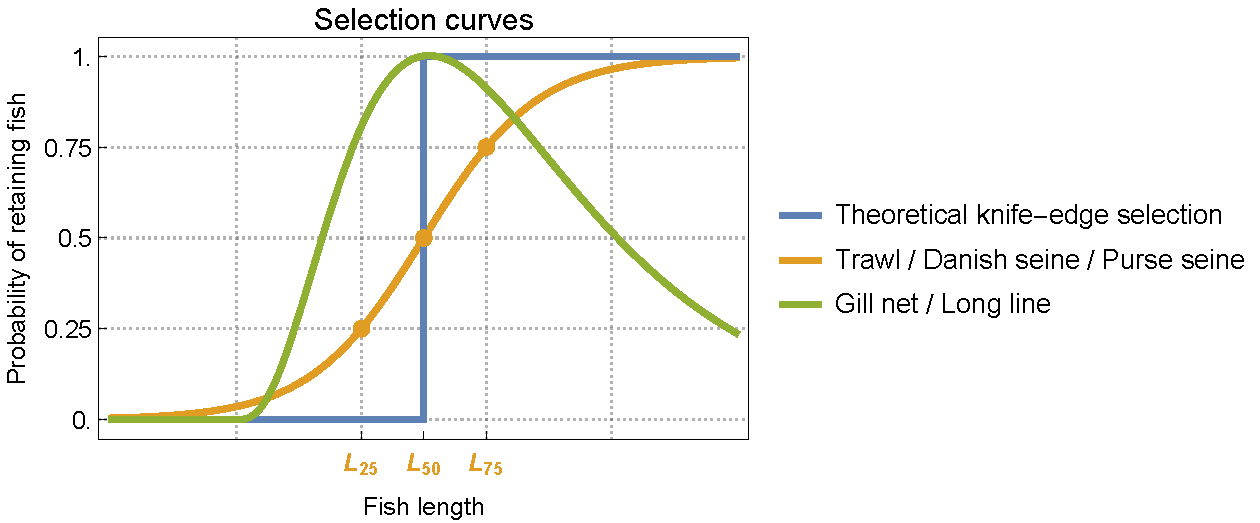
\includegraphics[scale=.7]{selection}
,\caption{The figure illustrates typical selection curves for gill nets and trawl gears. The fish lengths $L_{25}$, $L_{50}$ and $L_{75}$ are referring to the curve representing trawl (indicated by the three points), referring to percentage of the exposed fish retained and captured by the gear. However, this reference point is less useful when the selection curve has a declining trend by increasing length, as for gill net and long line. }
\label{fig:selection}
\end{figure}

Figure~\ref{fig:selection} displays three different selection curves. The knife-edge selection is an idealised selection curve which simplifies the problem of gear selection in models we discuss in this book. The idealised curve could be regarded as a special case of trawl selection (for simplicity we refer to trawls even though the curve also has relevance for a number of other gears, such as Danish seine and purse seine). While selection in the idealised curve (actually a piece-wise linear curve) is immediate, there is a movement over a range of fish lengths to get from 0 to 100\% selection in the more realistic curve. The range between $L_{25}$ (25\% retained) and $L_{75}$ (75\% retained) is often referred to as the \textit{Selection Range} (\textit{SR}).

The logistic equation is often assumed to capture the selection pattern of trawls and similar gears. This is the inverse version of the \textit{logit} function $log(x/(1-x))$ that follows a pattern very close to the \textit{probit} function we knows from probability theory and statistics. For the purpose of describing a pattern of selection it is convenient to express the logistic function by
\begin{equation} 
\label{eq:gearselection}
p(L) = \frac{e^{a + b L}}{1 + e^{a + b L}}
\end{equation}
(see also code box~\ref{code:verhulst} in the next chapter) where $a$ and $b$ are parameters defining $L_{50}$:
\begin{equation} 
L_{50} = - \frac{a}{b}
\end{equation}
$SR$ is defined by the parameter $b$:
\begin{equation} 
SR = \frac{2 \cdot log(3)}{b}
\end{equation}
when we assume SR to cover the 50\% between $L_{25}$ and $L_{75}$. $p(L)$ in equation~\ref{eq:gearselection} expressed the probability of catch when the fish has length $L$. From the equations above we see that $a$ and $b$ are determined when $L_{50}$ and $SR$ are given:
\begin{equation}
\label{eq:ablogistic}
\begin{aligned} & a = \frac{2 \cdot L_{50} \cdot log(3)}{SR} \\\\
& b = - \frac{a}{L_{50}}
\end{aligned}
\end{equation}

%------------------------------------------------
\section*{Exercises}\index{Exercises!Chapter 3}
\addcontentsline{toc}{section}{Exercises}

\begin{exercise}
Give alternative explanations on why effort-output-elasticities ($\alpha$ in equation~\ref{eq:cobbdouglas3}) could be larger than one.
\end{exercise}

\chapterimage{h4.jpg} % Chapter heading image

\chapter{Modelling population dynamics} \label{chapter 4}
%----------------------------------------------------------------------------------------
%	CHAPTER 4
%----------------------------------------------------------------------------------------
\section{Basic principles}
A group of individuals of the same species living in a specific geographically area is referred to as a population. Populations may be separated into smaller sub-populations (referred to as stocks) in minor geographical areas. Population dynamics describes how a population or stock grows due to the genetic properties of the population/stock and the environmental constraints within the area the population/stock is living. In the following we will not differentiate between populations and stocks.

Population growth is the net effect of individual growth, recruitment and mortality during a period of time. All these factors depend both of the biological properties of the species and of the physical and biological environment. The size of a population could be measured in numbers of individuals (the common measure in the human population) or in terms of weight (the common measure of fish stocks). The latter is often referred to as the stock's biomass, which is the total weight of the stock in nature.

The science of population dynamics originates from the same public discourse resulting in the discipline of economics and demographics at the end of the eighteenth century. Several of the mathematical demographic models we will discuss in this chapter originates from that period, at that time focusing the growth of the human population.

\begin{figure}[!htb]
\begin{remark}
\rule{\linewidth}{.1pt}
\floatbox[{\capbeside\thisfloatsetup{capbesideposition={right,top},capbesidewidth=11.8cm}}]{figure}[\FBwidth]
{\caption*{\footnotesize{Study how a human population grows according to \\ reproduction properties and generation time at

\href{http://demonstrations.wolfram.com/OffspringOfAdamAndEve/}{\\ http://demonstrations.wolfram.com/ \\ OffspringOfAdamAndEve/}}}}
{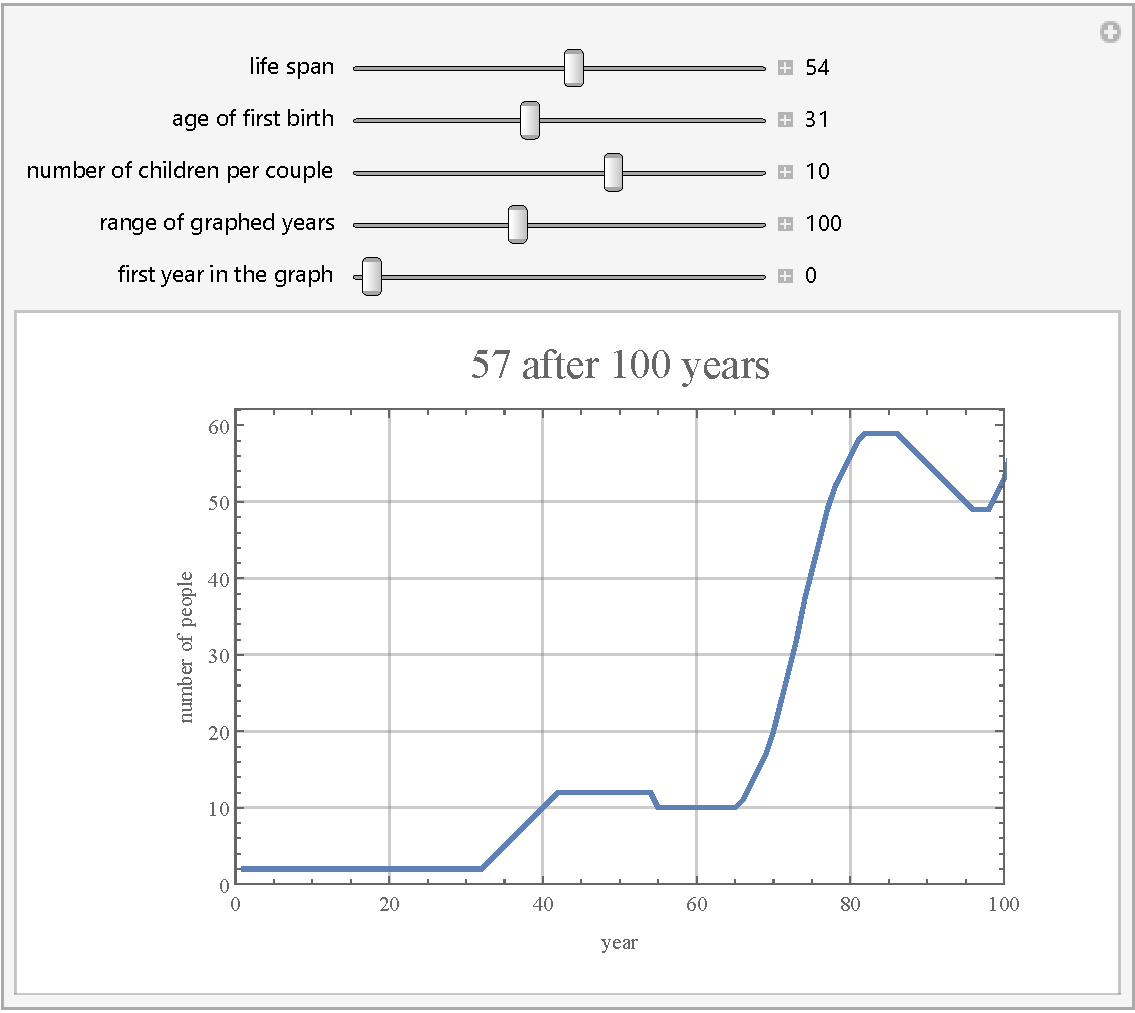
\includegraphics[width=2.8cm]{demo_AdamEve}}\\
\rule[10pt]{\linewidth}{.1pt}
\end{remark}
\end{figure}

%------------------------------------------------
\section{Classical surplus growth models}\label{section:surplus production}

Of course people had been interested in and fascinated by population growth long time before the eighteenth century. One example is the Fibonacci numbers, described by an Italian mathematician (Leonardo of Pisa Bonacci, about 1170 – about 1250)) during the first years of the thirteenth century (the series has however been known from ancient times). 

The Fibonacci numbers describes biological growth starting with a newborn pair of rabbits (1). At the end of the first month they mate and a new pair is born at the end of the second month. Then there are two pairs. The first pair gives birth to a new pair every month (mortality is not existing in this model), while the second pair starts mating as the first pair after their first month. The Fibonacci series then gives the monthly number of pairs of rabbits.

\begin{theorem}[Fibonacci numbers]
\hfill \break
In \textit{Mathematica} you have an internal function listing the Fibonacci numbers:
\index{\texttt{Table}}\index{\texttt{Fibonacci}}
\begin{mmaCell}[index=1]{Input}
  Table[Fibonacci[n], \{n, 20\}]
\end{mmaCell}
\begin{mmaCell}{Output}
  \{1, 1, 2, 3, 5, 8, 13, 21, 34, 55, 89, 144, 233, 377, 
  610, 987, 1597, 2584, 4181, 6765\}
\end{mmaCell}
\index{\texttt{ListLinePlot}}
\begin{mmaCell}{Input}
  ListLinePlot[\%1, Mesh -> All, PlotRange -> All, Filling -> Axis]
\end{mmaCell}
\begin{mmaCell}[moregraphics={moreig={scale=.7}}]{Output}
  \mmaGraphics{fibongrowth}
\end{mmaCell}
Now have a look at the ratio between two and two consecutive numbers
\index{\texttt{Range}}
\begin{mmaCell}{Input}
  Fibonacci[# + 1]/Fibonacci[#] & /@ Range[20]
\end{mmaCell}
\begin{mmaCell}{Output}
  \Big\{1, 2, \mmaFrac{3}{2}, \mmaFrac{5}{3}, \mmaFrac{8}{5}, \mmaFrac{13}{8}, \mmaFrac{21}{13}, \mmaFrac{34}{21}, \mmaFrac{55}{34}, \mmaFrac{89}{55}, \mmaFrac{144}{89}, \mmaFrac{233}{144}, \mmaFrac{377}{233}, \mmaFrac{610}{377},
  \hfill \break
  \mmaFrac{987}{610}, \mmaFrac{1597}{987}, \mmaFrac{2584}{1597}, \mmaFrac{4181}{2584}, \mmaFrac{6765}{4181}, \mmaFrac{10946}{6765}\Big\} 
\end{mmaCell}
The numerical values reveal that the ratios soon approach the same value while moving upwards in the series.
\index{\texttt{N} (Numeric)}
\begin{mmaCell}{Input}
  N[\%]
\end{mmaCell}
\begin{mmaCell}{Output}
  \{1., 2., 1.5, 1.66667, 1.6, 1.625, 1.61538, 1.61905, 1.61765, 
  1.61818, 1.61798, 1.61806, 1.61803, 1.61804, 1.61803, 1.61803, 
  1.61803, 1.61803, 1.61803, 1.61803\} 
\end{mmaCell}
Let us look at the numerical value of the built in function \texttt{GoldenRatio}, and we obtain the same number.
\index{\texttt{GoldenRatio}}\index{\texttt{N} (Numeric)}
\begin{mmaCell}{Input}
  GoldenRatio // N
\end{mmaCell}
\begin{mmaCell}{Output}
  1.61803 
\end{mmaCell}
\index{\texttt{Show}}\index{\texttt{Plot}}\index{\texttt{ListLinePlot}}
\begin{mmaCell}{Input}
  Show[\{
    ListLinePlot[\%3, PlotRange -> All, Mesh -> All],
    Plot[GoldenRatio, \{n, 0, 20\}, PlotStyle -> Red]
  \}]
\end{mmaCell}
\begin{mmaCell}[moregraphics={moreig={scale=.8}}]{Output}
  \mmaGraphics{fibon}
\end{mmaCell}
The blue curve (\texttt{Out[3]} falls together with the red curve (the golden ratio, \texttt{Out[4]}). The golden ratio therefore could be obtained directly from the Fibonacci numbers:
\index{\texttt{Limit}}\index{\texttt{Fibonacci}}
\begin{mmaCell}{Input}
  Limit[Fibonacci[n + 1]/Fibonacci[n], n -> Infinity]
\end{mmaCell}
\begin{mmaCell}{Output}
  \mmaFrac{1}{2} \Big(1 + \mmaSqrt{5}\Big) 
\end{mmaCell}
Let us complete this session with the Fibonacci numbers by looking at one of many examples of how these numbers produce beautiful patterns in the nature. Here we use the golden ratio to draw patterns found in sunflower heads and compare it with a real flower:
\index{\texttt{Table}}\index{\texttt{Graphics}}\index{\texttt{GraphicsRow}}\index{\texttt{ImageCrop}}\index{\texttt{Point}}\index{\texttt{Import}}
\begin{mmaCell}{Input}
  GraphicsRow[\{
    Show[
      Graphics[\{
        Lighter@Yellow, AbsolutePointSize[3 + #^(1/3)/2],
        Point[
          Sqrt[#]\{Cos[2 Pi # GoldenRatio],Sin[2 Pi # GoldenRatio]\}
        ]\}
      ] & /@ Range[360],
      Graphics[\{Lighter@Yellow, Annulus[\{0, 0\}, \{19, 30\}]\}]\},
      Background -> Darker@Brown,
      PlotRange -> \{\{-20, 20\}, \{-20, 20\}\} ], 
    ImageCrop[Import["https://c1.staticflickr.com/2/
      1278/694780262_8874b4f225_b.jpg"], \{600, 600\}]
  \}]
\end{mmaCell}
\begin{mmaCell}[moregraphics={moreig={scale=.7}}]{Output}
  \mmaGraphics{sunflower}
\end{mmaCell}
\label{code:fibonacci}
\end{theorem}
\hfill \break
An interesting feature of the series is that each number is equal the sum of the two previous numbers. At first sight the series may appear to be rather randomly constructed but it is following a strict rule where the population of rabbits after only a few months reach astronomical values. The series is a simple recruitment model and does not include growth in biomass and mortality. It demonstrates however the exponential power of population growth which was also discovered in European countries during the eighteenth century.

The British scholar Thomas Robert Malthus (1766 - 1834) claimed that the exponential increase in the human populations throughout Europe in the eighteenth century eventually would be repressed at a maximum level (the level of subsistence) where the human population would suffer at the edge of the nature's capacity level of sustaining the large human population.

Malthus' ideas became very influential but were also criticised by many. The idea that there existed an upper limit for how large a human population could be, and that this limit was related to environmental constraints (e.g. food), was however shared by most of the critics.

\begin{theorem}[Gompertz' population growth model]
\hfill \break
The Gompertz equation~\ref{eq:gompertz} is solved by \textit{Mathematica} while providing a value for the initial stock biomass ($X_0$, implemented below as x0). The solution includes a message indicating that other solutions may exist in the general case of such
\index{\texttt{DSolve}}\index{\texttt{Log}}
\begin{mmaCell}[index=1]{Input}
  DSolve[
    \{x'[t] == -r x[t] Log[x[t]/k], x[0] == x0\}, x[t], t
  ][[1, 1]]
\end{mmaCell}
\begin{mmaCell}[messagelink=message/General/infy]{Message}
  Solve::ifun: Inverse functions are being used by Solve, so some solutions may 
  not be found; use Reduce for complete solution information. >>
\end{mmaCell}
\begin{mmaCell}{Output}
  x[t] \(\to\) k \mmaSup{\bigg(\mmaFrac{x0}{k}\bigg)}{\mmaSup{e}{-r t}}
\end{mmaCell}
Plotting equation~\ref{eq:gompertz} (left below) and its solution (right below) for some given parameter values ($r = 0.5$, $K = 1000$ and $X_0 = 10$)
\index{\texttt{Plot}}\index{\texttt{GraphicsRow}}\index{\texttt{Log}}
\begin{mmaCell}{Input}
  GraphicsRow[\{
    Plot[-.5 x Log[x/1000], \{x, 0, 1000\}],
    Plot[1000 (10/1000)^Exp[-.5 t], \{t, 0, 12\}]
  \}]
\end{mmaCell}
\begin{mmaCell}[moregraphics={moreig={scale=.8}}]{Output}
  \mmaGraphics{gompertzcurve}
\end{mmaCell}
\label{code:gompertz}
\end{theorem}
\hfill \break
\index{Surplus production!Gompertz model}Benjamin Gompertz (1779 – 1865) published in 1825\cite{Gompertz1825} a mathematical demographic model. When replacing the variable (numbers of peoples) with a stock's biomass ($X$), the Gompertz' growth equation gives the time derivative of the stock biomass
\begin{equation} 
\label{eq:gompertz}
\dot{X}(t) = \frac{dX(t)}{dt} = - r \cdot X(t) \cdot ln\Big(\frac{X(t)}{K}\Big)
\end{equation}
where $r$ is a growth rate while $K$ is the environmental carrying capacity level. Since the time derivative is the per unit of time increment in the stock biomass, it provides a straight forward biological interpretation on the speed by which the stock grows towards its natural equilibrium $K$. As seen from the plot of equation~\ref{eq:gompertz} in Code box~\ref{code:gompertz}, the point of maximum growth is placed to the left of $K/2$.

Another demographic model, published only a few years after the Gompertz model, and with an even greater scientific impact, was suggested by \index{Surplus production!Verhulst model}Pierre François Verhulst (1804 - 1849) in 1838 \cite{Verhulst1838}. It is commonly referred to as the logistic growth equation and in line with the expression above it may be written as:
\begin{equation} 
\label{eq:verhulst}
\dot{X}(t) = r \cdot X(t) \Big(1 - \frac{X(t)}{K}\Big)
\end{equation}
As seen from equation~\ref{eq:verhulst} (and illustrated in Code box~\ref{code:verhulst}) the time derivative of the logistic growth describes a parabolic curve. The inflection point of $X(t)$ therefore is found for $X(t) = K/2$. After Raymond Pearl (1879 -- 1940) in 1925 re-introduced the logistic growth curve as a biomass surplus growth model\cite{Pearl1925} it has become the most common surplus growth model used in mathematical biology and fisheries economics.

\begin{theorem}[Verhults population growth model]
\hfill \break
The Verhulst equation~\ref{eq:verhulst} is solved by \textit{Mathematica} while providing a value for the initial stock biomass ($X_0$, below represented by \texttt{x0}). The solution includes a message indicating that other solutions may exist in the general case of such
\index{\texttt{DSolve}}
\begin{mmaCell}[index=1]{Input}
  DSolve[\{x'[t]== r x[t](1-x[t]/k), x[0]== x0\}, x[t], t][[1, 1]]
\end{mmaCell}
\begin{mmaCell}[messagelink=message/General/infy]{Message}
  Solve::ifun: Inverse functions are being used by Solve, so some solutions may 
  not be found; use Reduce for complete solution information. >>
\end{mmaCell}
\begin{mmaCell}{Output}
  x[t] \(\to\) \mmaFrac{\mmaSup{e}{rt} k x0}{k - x0 + \mmaSup{e}{rt} x0}
\end{mmaCell}
Plotting equation~\ref{eq:verhulst} (left below) and its solution (right below) for some given parameter values ($r = 0.5$, $K = 1000$ and $X_0 = 10$)
\index{\texttt{Plot}}\index{\texttt{GraphicsRow}}\index{\texttt{Exp}}
\begin{mmaCell}{Input}
  GraphicsRow[\{
    Plot[.5 x (1 - x/1000), \{x, 0, 1000\}],
    Plot[(Exp[.5t]1000 * 10)/(1000 - 10 + Exp[.5t]10), \{t, 0, 20\}]
  \}]
\end{mmaCell}
\begin{mmaCell}[moregraphics={moreig={scale=.8}}]{Output}
  \mmaGraphics{verhulstcurve}
\end{mmaCell}
The dynamics of the logistic function is studied in a vast number of papers and the chaotic properties of the function is well-known. The discrete version of the model exhibit in particular dynamic changes depending on the value of the intrinsic growth parameter $r$. To investigate how the growth pattern changes according to the value of $r$ the discrete model is plotted below for three $r$-values, 0.5, 2.5 and 3.0. The plots below show how the stock biomass ($X$) varies over time ($t$, the horizontal axis).
\index{\texttt{Table}}\index{\texttt{GraphicsRow}}\index{\texttt{ListLinePlot}}\index{\texttt{NestList}}
\begin{mmaCell}{Input}
  GraphicsRow[Table[
    ListLinePlot[
      NestList[# + r # (1 - #/1000.) &, 100, 50], 
      PlotStyle -> Directive[\{Thickness[.01], Red\}],
      PlotRange -> \{0, 1400\}
    ], 
    \{r, \{.5, 2.5, 3\}\}
  ]]
\end{mmaCell}
\begin{mmaCell}[moregraphics={moreig={scale=1}}]{Output}
  \mmaGraphics{discretelogistic1}
\end{mmaCell}
The dynamics above can be presented as cobweb diagram, as shown below. The cobweb diagrams display the changes over time in $x(t)-x(t+1)$-axes-systems. The yellow lines below correspond to $x(t) = x(t+1)$ (equilibrium).
\index{Surplus production!Cobweb diagram}\index{\texttt{NestList}}\index{\texttt{Show}}\index{\texttt{Plot}}\index{\texttt{RotateLeft}}\index{\texttt{GraphicsRow}}\index{\texttt{ListLinePlot}}\index{\texttt{Riffle}}
\begin{mmaCell}{Input}
  GraphicsRow[Table[
    Show[\{
      Plot[\{x+r x(1-x/1000.), x\}, \{x,0,1400\}],
      ListLinePlot[(
        nested = NestList[#+r # (1-#/1000.)\&, 100, 50];
        nested = Riffle[
          \{#, #\}\& /@ nested, 
          Table[Take[RotateLeft[#,i],2], \{i, 0, 49\}]\& @ nested
        ]), 
        PlotRange -> All
      ]\}, 
      AspectRatio -> 1,
      PlotStyle   -> Directive[\{Thickness[.01], Red\}], 
      PlotRange   -> \{0,All\}
    ],
    \{r, \{.5, 2.5, 3\}\}
  ]]
\end{mmaCell}
\begin{mmaCell}[moregraphics={moreig={scale=.6}}]{Output}
  \mmaGraphics{discretelogistic2}
\end{mmaCell}
While the left hand figure reflects smooth growth towards the equilibrium ($X = K$, in this case the value 1000), the graph in the middle ($r = 2.5$) displays that the equilibrium is an eight-periodic orbit around a stable focus (which in continuous time corresponds to a two-period limit cycle), while the right hand figure displays a chaotic situation.
\label{code:verhulst}
\end{theorem}
\hfill \break
\index{Surplus production!Richards model}In 1959 F. J. Richards (1901 – 1965) published a model in which the two previously presented models (equations~\ref{eq:gompertz} and~\ref{eq:verhulst}) are special cases, referring to it as \textit{a flexible growth function for empirical use}\cite{Richards1959}. In line with the previous equations we express Richards function in this way
\begin{equation} 
\label{eq:richards}
\dot{X}(t) = r \cdot X(t) \bigg( 1 - \bigg(\frac{X(t)}{K}\bigg)^{m - 1} \bigg),
\end{equation}
introducing a third parameter ($m$), which moves the inflection point of the growth upwards and downwards depending on its value. It is easy to see that equation~\ref{eq:richards} is equal equation~\ref{eq:verhulst} for $m = 2$. It is also possible to show that equation~\ref{eq:richards} actually approaches equation~\ref{eq:gompertz} when $m$ approaches one. Then both the Gompertz growth and the Verhulst growth equations are special cases of the Richards growth in equation~\ref{eq:richards}. The graph shown in Code box~\ref{code:growth} illustrates how the $m$-parameter in the Richards growth equation determines if the growth curve should be squeezed to the left or the right. 

\begin{theorem}[Surplus growth models]
\hfill \break 
This session makes use of the package \texttt{PopulationGrowth} (freely available at \\ http://site.uit.no/econmult/). If the package is found by \textit{Mathematica} in its file system, it is loaded by the command:
\index{\texttt{Needs}}
\begin{mmaCell}[index=1]{Input}
  Needs["EconMult`PopulationGrowth`"]
\end{mmaCell}
This lists four surplus production models available in the package:
\index{\texttt{Text}}\index{\texttt{Grid}}
\begin{mmaCell}{Input}
  Grid[
    Text /@ \{#, 
      Notation@SurplusProduction[UseMSY->False, GrowthModel->#],
      SimplifyNotation@SurplusProduction[GrowthModel -> #]
    \} & /@ \$SurplusProductionModels, 
    Frame     -> All, 
    Alignment -> Left
  ]
\end{mmaCell}
\begin{mmaCell}[moregraphics={moreig={scale=1.2}}]{Output}
  \mmaGraphics{growthmodels}
\end{mmaCell}
\index{\texttt{Table}}\index{\texttt{Show}}\index{\texttt{Plot}}
\begin{mmaCell}{Input}
  Show[(
    Plot[
      SurplusProduction[
        GrowthModel                     -> RichardsPellaTomlinson, 
        CurrentBiomass                  -> x, 
        UseMSY                          -> True, 
        MaximumSustainableYield         -> 100, 
        CatchabilityCoefficient         -> 1, 
        BiomassMaximum                  -> 1000,
        RichardsPellaTomlinsonParameter -> #
      ], \{x, 0, 1000\}, 
      PlotRange        -> \{0, 100\}, 
      Frame            -> True, 
      FrameLabel       -> \{"Stock size",
        "Natural growth per unit of time"\}, 
      PlotRangePadding -> None
    ] &) /@ Table[Exp[.001 + .1 * i^3] - 1, \{i, 0, 4, .5\}]
  ]
\end{mmaCell}
\begin{mmaCell}[moregraphics={moreig={scale=.9}}]{Output}
  \mmaGraphics{growthmodels2}
\end{mmaCell}
\label{code:growth}
\end{theorem}

\begin{figure}[!htb]
\begin{remark}
\rule{\linewidth}{.1pt}
\floatbox[{\capbeside\thisfloatsetup{capbesideposition={right,top},capbesidewidth=11.8cm}}]{figure}[\FBwidth]
{\caption*{\footnotesize{Investigate the cobweb map of a logistic growth equation:

\href{http://demonstrations.wolfram.com/AnIntervalEventuallyBoundingTrajectoriesOfTheLogisticMap/}{\\ http://demonstrations.wolfram.com/\\AnIntervalEventuallyBoundingTrajectoriesOfTheLogisticMap/}}}}
{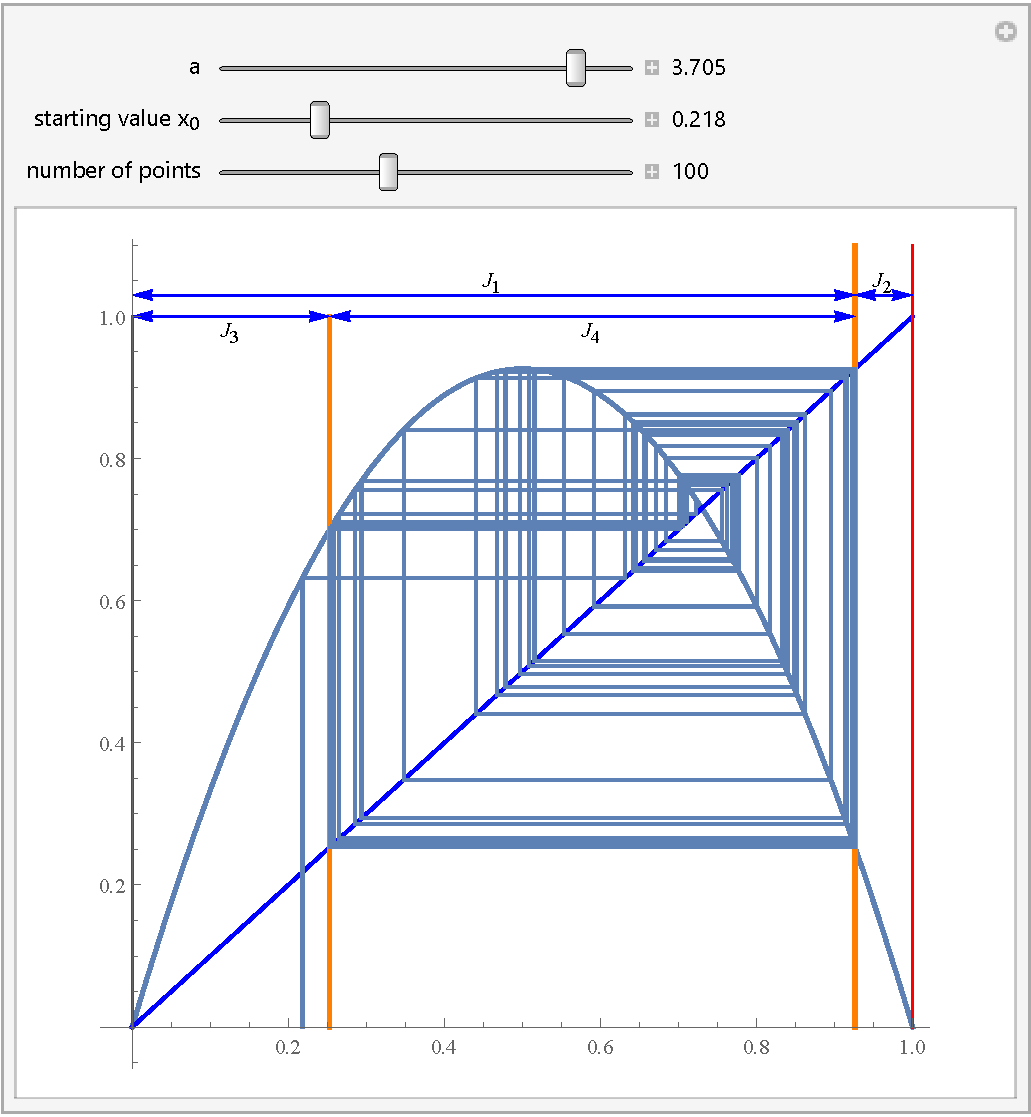
\includegraphics[width=2.8cm]{demo_LogisticGrowth}}\\
\rule[10pt]{\linewidth}{.1pt}\end{remark}\end{figure}
%------------------------------------------------

\section{Depensatory growth}\label{section:depensatory growth}\index{Surplus production!Depensatory growth}

The models introduced in section~\ref{section:surplus production} above are all included in the class of compensatory growth models. The term \textit{compensatory} refers to the fact that in these models the relative growth rate ($\dot{X}(t)/X(t)$) is increasing for decreasing stock biomass levels. Biomass losses leads to an increasing compensation per unit of biomass.

This kind of compensating behaviour in the stock may however not always be the case in real life. The relative growth rate may increase by decreasing stock biomass down to a certain level where the relative growth rate also decreases. It may even turn negative in some cases. These cases are referred to as critical depensation, defining a critical biomass level below which the stock will go extinct.

A depensatory growth model may be specified on the basis of the logistic equation~\ref{eq:verhulst} by adding a term including a depensation parameter $D$:
\begin{align*}
\dot{X}(t) = r \cdot X(t)  \Big(1 - \frac{X(t)}{K}\Big) \cdot \frac{X(t) - D}{K - D}
\end{align*}
which gives
\begin{equation} 
\label{eq:depensationverhulst}
\dot{X}(t) = \frac{r \cdot X(t) \cdot \big(K-X(t)\big) \cdot \big(X(t)-D\big) }{K \cdot \big(K-D\big)}
\end{equation}
If the depensation parameter $D$ is negative the depensation is non-critical, while the interpretation of a positive depensation parameter is the critically low biomass level. By the use of \textit{Mathematica} it is easy to show that $D = -\infty$ restores equation~\ref{eq:verhulst}:
\index{\texttt{Limit}}
\begin{mmaCell}[index=1]{Input}
  Limit[(r x (k - x) (x - d))/(k (k - d)), d -> -Infinity]
\end{mmaCell}
\begin{mmaCell}{Output}
   \mmaFrac{r (k - x) x}{k}
\end{mmaCell}

\begin{theorem}[Depensatory growth]
\hfill \break
Depensatory growth as expressed in equation~\ref{eq:depensationverhulst} includes both critical and non-critical depensation levels. The plot of equation~\ref{eq:depensationverhulst} (below) for different $D$-values illustrates this. The chosen colours goes from non-critical (blue) to critical (red) depensation levels.
\index{\texttt{Show}}\index{\texttt{Plot}}\index{\texttt{Log}}\index{\texttt{Hue}}
\begin{mmaCell}[index=1]{Input}
  Show[
    Plot[
      r x(k-x)(x-d))/(k(k-d)) /. \{r->.5, k->1000, d->#\},
      \{x, 0, 1000\},
      PlotStyle -> Hue[.8 - Abs[Log[2 + #/3000]]]
    ] & /@ \{-50000, -3000, -1000, -300, 0, 200, 400\}, 
    PlotRange -> All,
    AxesLabel -> \{"X", "dX/dt"\}
  ]
\end{mmaCell}
\begin{mmaCell}[moregraphics={moreig={scale=.7}}]{Output}
  \mmaGraphics{depensation}
\end{mmaCell}
Two of the $D$-values above are positive and hence defining critical biomass levels, respectively for stock sizes of 200 and 400. The blue curve ($D = -50,000$) is approaching the logistic growth function (obtained when $D = -\infty$).

The plot below shows the relative growth (or average growth; surplus production per unit of biomass) for the $D$-values included in the plot above.
\index{\texttt{Show}}\index{\texttt{Plot}}\index{\texttt{Log}}\index{\texttt{Hue}}
\begin{mmaCell}[index=1]{Input}
  Show[
    Plot[
      r x(k - x)(x - d))/(k(k - d))/x /. \{r ->.5, k ->1000, d ->#\},
      \{x, 0, 1000\}, 
      PlotStyle -> Hue[.8 - Abs[Log[2 + #/3000]]]
    ] & /@ \{-50000, -3000, -1000, -300, 0, 200, 400\}, 
    PlotRange -> All, 
    AxesLabel -> \{"X", "(dX/dt)/X"\}
  ]
\end{mmaCell}
\begin{mmaCell}[moregraphics={moreig={scale=.7}}]{Output}
  \mmaGraphics{relativegrowthdepensation}
\end{mmaCell}
We see that the two orange or red curves, representing the two cases of critical depensation, becomes negative at sufficiently low $D$-values. Other cases also indicate depensation but not all of them. The blue and magenta coloured curves obviously shows an increasing trend by decreasing $D$-values in the whole range of $D$-values. This also seems to be the case for the green curve.  

The plot below gives the marginal values of the relative growth, with respect of stock biomass $X$. This plot confirms that the blue, magenta and green curves indeed belong to the class of compensatory growth models, while the other cases belong to the class of depensatory growth models. We base this conclusion on the fact that the first three cases do not enter the positive region of marginal relative growth. Among the depensatory growth cases the orange (red) curves represent critical depensatory growth, while the other two (the yellow curves) represent depensatory growth where no critical biomass values above zero are found.
\index{\texttt{D} (Derivative)}\index{\texttt{Plot}}\index{\texttt{Log}}\index{\texttt{Abs}}\index{\texttt{Hue}}
\begin{mmaCell}[index=1]{Input}
  Show[
    Plot[
      D[r x(1 - x/k)(x - d)/(k - d)/x, x] /. 
      \{r -> .5, k -> 1000, d -> #, x -> y\}, \{y, 0, 1000\}, 
      PlotStyle -> Hue[.8 - Abs[Log[2 + #/3000]]]
    ] & /@ \{-50000, -3000, -1000, -300, 0, 200, 400\}, 
    PlotRange -> All, AxesOrigin -> \{0, 0\}, 
    AxesLabel -> \{"X", "-(dX/dt)/\mmaSup{X}{2}"\}
  ]
\end{mmaCell}
\begin{mmaCell}[moregraphics={moreig={scale=.7}}]{Output}
  \mmaGraphics{marginaldepensation}
\end{mmaCell}
The curves intersections with the horizontal axis corresponds to the maximum values of the relative growth. While the green curve reach zero at $D = 0$, the magenta and blue curves do not reach positive values for $D \geq 0$.

Analytically it is possible to prove that the range of $D$-values of compensatory growth is from $-\infty$ to $-K$, non-critical depensatory growth goes from $-K$ to $0$, while the critical area lays in the interval of $D$-values between $0$ and $K$, being the maximum biomass level.
\label{code:depensation}
\end{theorem}

Most all examples provided in this text book assume compensatory growth. Shifting to depensatory growth may severely alter the conclusions of the compensatory growth models. If the stock's ability to strive for increased growth per biomass unit with declining stock size is weakened,  consequences of overfishing may be much more severe.

In the next section age structure models are introduced. Walters et al. (2008)\cite{Walters2008} discusses the relationship between depensatory growth in surplus production models versus age structured models and claims that depensation is more commonly included in age structured models.

%------------------------------------------------

\section{Age structured model}\index{Cohort models}\label{section:age structured model}

Age structured population models decompose the population biomass to different age components, each of them being the product of average individual weight in the age group and number of individuals. Changes in age composition of the stock will affect the stock biomass development in ways not necessarily grasped by the surplus production models presented in section~\ref{section:surplus production}.

Age structured models are often referred to as cohort models, a more general term which allows the stock to be structured in other ways that by year classes, which is the normal structure. For some species, however, structuring by other time intervals (for example by month) or more aggregated groups (for example mature and immature individuals) is preferable to structuring by year-classes.

In 1934 Karl Ludwig von Bertalanffy (1901 -- 1972) launched an individual length growth model for asymptotic growth towards a maximum length ($L_\infty$) by increasing age\cite{Bertalanffy1934}. Let $L(t)$ be the individual length at age $t$, $k$ the length growth rate and $t_0$ the theoretical age of zero length ($L(t_0) = 0$). The von Bertalanffy equation is then given by
\begin{equation} 
\label{eq:vonbertalanffyL}
L(t) = L_\infty \big(1 - e^{-k(t-t_0)}\big)
\end{equation}
The weight growth is closely related to length growth. Let parameter $b$ represent the weight/length relationship and $d$ be a scaling factor. The individual weight at age $t$, $W(t)$, then is given by
\begin{equation} 
\label{eq:vonbertalanffyW}
W(t) = d\cdot L(t)^b
\end{equation}
Maximum individual weight also is defined by equation~\ref{eq:vonbertalanffyW}, $W_\infty = d \cdot L_\infty^b$. Inserting equation~\ref{eq:vonbertalanffyL} in equation~\ref{eq:vonbertalanffyW} then gives\footnote{Taking the time derivative of this function shows that the function in fact is a Richards equation (equation~\ref{eq:richards}).}
\begin{equation} 
\label{eq:vonbertalanffy}
W(t) = W_\infty \big(1 - e^{-k(t-t_0)}\big)^b
\end{equation}

\begin{corollary}[Parameter relations]
\hfill \break
\small{\indent Some will emphasise that the gain of moving from aggregated surplus production models to cohort models is clearer biological interpretations of the model parameters.

The growth rate $k$ is the percentage increment in length in relation to the difference between maximum length and current length. This gives a constant percentage of a diminishing difference, hence the length growth is approaching zero as the length approaches $L_\infty$.
\begin{align*}
k = \frac{\dot{L}(t)}{L_\infty - L(t)}
\end{align*}
$b$ is the ratio between the percentage growth in weight and the percentage growth of length at the same age. This ratio is assumed to be constant and usually close to 3, being the cubic expansion of length.
\begin{align*}
b = \frac{\dot{W}(t)}{W(t)} \bigg/ \frac{\dot{L}(t)}{L(t)}
\end{align*}
$d$ is simply a scaling parameter which value depends on the units by which weight and length are measured.
\begin{align*}
d = \frac{W_\infty}{{L_\infty}^b}
\end{align*}

The mortality rate $Z$ gives a constant percentage decline in the number of individuals by age. On basis of the relations above the mortality rate may also be expressed in terms of percentage increment in weight minus percentage increment in biomass in a cohort.
\begin{align*}
Z = - \frac{\dot{N}(t)}{N(t)} = \frac{\dot{W}(t)}{W(t)} - \frac{\dot{x}(t)}{x(t)} = b \cdot \frac{\dot{L}(t)}{L(t)} - \frac{\dot{x}(t)}{x(t)}
\end{align*}
}
\label{code:k}
\end{corollary}
\hfill \break
While the individual weight increases by age, the number of individuals of a cohort decreases over time due to natural mortality (predation, age and diseases). The standard mortality model was first proposed by Baranov in 1918\cite{Baranov1918}. If $R$ is the initial number of recruits in a cohort (at the age of recruitment, $t_R$) and the mortality rate is $Z$, then the number of individuals in the cohort at time $t$, $N(t)$, is
\begin{equation} 
\label{eq:baranov}
N(t) = R \cdot e^{-Z(t-t_R)}
\end{equation}
The product of equations~\ref{eq:vonbertalanffyW} and~\ref{eq:baranov} gives the total biomass of the cohort in question:
\begin{equation} 
\label{eq:cohort}
x(t) = N(t) \cdot W(t) = R  \cdot W_\infty \cdot \big(1 - e^{-k(t-t_0)}\big)^b \cdot e^{-Z(t-t_R)}
\end{equation}

\begin{theorem}[Biomass of one cohort and all cohorts]
\hfill \break 
This session makes use of the package \texttt{PopulationGrowth} (freely available at \\ \textit{http://www.maremacentre.com/econmult}). If the package is found by \textit{Mathematica} in its file system, it is loaded by the command:
\index{\texttt{Needs}}
\begin{mmaCell}[index=1]{Input}
  Needs["EconMult`PopulationGrowth`"]
\end{mmaCell}
The von Bertalanffy equation (equation~\ref{eq:vonbertalanffy}) is implemented in the package as:
\begin{flushleft}
\begin{mmaCell}{Input}
  IndividualWeight[t] // Notation
\end{mmaCell}

\includegraphics[scale=.85]{pg1}

By default the package assumes the total mortality rate ($Z$, as in equation~\ref{eq:baranov}) to be the sum of $F$ and $M$, respectively the fishing and natural mortality rate (see equation~\ref{eq:mortality}). The Baranov equation (equation~\ref{eq:baranov}) therefore is implemented by
\begin{mmaCell}{Input}
  IndividNumbers[t] // Notation
\end{mmaCell}

\includegraphics[scale=.85]{pg2}

The product of number of individuals ($N$) and individual weigh ($W$) gives the biomass of the cohort (equation~\ref{eq:cohort}):
\begin{mmaCell}{Input}
  CohortBiomass[t] // Notation
\end{mmaCell}

\includegraphics[scale=.85]{pg3}

Maximum biomass of cohort is found by
\index{\texttt{Solve}}
\begin{mmaCell}{Input}
  Solve[CohortBiomass'[t] == 0, t] // SimplifyNotation
\end{mmaCell}
\begin{mmaCell}[messagelink=message/General/infy]{Message}
  Solve::ifun: Inverse functions are being used by Solve, so some solutions may 
  not be found; use Reduce for complete solution information. >>
\end{mmaCell}

\includegraphics[scale=.85]{pg4}

This value of $t$ is implemented in the \texttt{PopulationGrowth} package as \texttt{AgeOfMaxGrowth}, the age at which the cohort has its maximum biomass.
\begin{mmaCell}{Input}
  AgeOfMaxGrowth[] // Notation
\end{mmaCell}

\includegraphics[scale=.85]{pg6}

Maximum biomass of cohort could then be found by
\begin{mmaCell}{Input}
  CohortBiomass[AgeOfMaxGrowth[]] // Notation
\end{mmaCell}

\includegraphics[scale=.85]{pg7}

The maximum biomass is implemented in the package by \texttt{MaximumBiomassGrowth}. This tests that \texttt{MaximumBiomassGrowth} actually is equivalent to \texttt{CohortBiomass[AgeOfMaxGrowth[]]}:
\begin{mmaCell}{Input}
  MaximumBiomassGrowth[] === CohortBiomass[AgeOfMaxGrowth[]]
\end{mmaCell}
\begin{mmaCell}{Output}
  True
\end{mmaCell}
We assume some numerical values to parametrise the model. The previously presented parameters are represented in the package by descriptive names: \texttt{InitialAge} ($t_0$), \texttt{WeightLengthRelation} ($b$), \texttt{MaxWeight} ($W_\infty$), \texttt{GrowthRate} ($k$), \texttt{MortalityRate} ($M$, a component of $Z$), \texttt{FishingMortalityRate} ($F$, a component of $Z$), \texttt{Recruits} ($R$) and \texttt{RecruitmentAge} ($t_R$). Some parameters are to be introduced later: \texttt{OldestAge} (age of oldest cohort in the stock, $t_\infty$) and \texttt{CatchAge} (age of first catch, $t_c$).
\begin{mmaCell}{Input}
  values = \{
    InitialAge           -> 0, 
    WeightLengthRelation -> 3, 
    MaxWeight            -> 10, 
    GrowthRate           -> .2, 
    MortalityRate        -> .2,
    FishingMortalityRate -> F, 
    Recruits             -> 1, 
    RecruitmentAge       -> 0, 
    CatchAge             -> tc, 
    OldestAge            -> Infinity\};
\end{mmaCell}
Without fishing the cohort has its maximum biomass at a age close to seven years:
\index{\texttt{Sequence}}
\begin{mmaCell}{Input}
  AgeOfMaxGrowth[Sequence @@ values, Fishing -> False]
\end{mmaCell}
\begin{mmaCell}{Output}
  6.93147
\end{mmaCell}
This gives a graphical illustration on how the biomass develops over the life span of the cohort, when assuming no fishing:
\index{\texttt{Plot}}
\begin{mmaCell}{Input}
  Plot[
    CohortBiomass[t, Sequence @@ values, Fishing -> False],
    \{t, 0, 20\}, 
    AxesLabel -> \{"Biomass of cohort", "Age"\}
  ]
\end{mmaCell}
\begin{mmaCell}[moregraphics={moreig={scale=.6}}]{Output}
  \mmaGraphics{pg8}
\end{mmaCell}
Now assume that a similar cohort is recruited to the stock every year after the first one:
\index{\texttt{Range}}\index{\texttt{Show}}\index{\texttt{Plot}}
\begin{mmaCell}{Input}
  Show[
    Plot[
      CohortBiomass[
        t - #, 
        Sequence @@ values, 
        Fishing -> False
      ], \{t, 0, 30\}, 
      AxesLabel -> \{"Year", "Biomass of cohort"\}, 
      PlotRange -> \{0, All\}
    ] & /@ Range[0, 30]
  ]
\end{mmaCell}
\begin{mmaCell}[moregraphics={moreig={scale=.6}}]{Output}
  \mmaGraphics{pg9}
\end{mmaCell}
By adding the biomass of all cohorts for each year we find how the stock biomass grows from the first cohort to a fully recruited stock. Negative biomass values are not possible and are ignored by using the \texttt{Max} function, assuming zero to be the lowest possible biomass value:
\index{\texttt{Table}}\index{\texttt{Max}}\index{\texttt{Total}}\index{\texttt{Sequence}}\index{\texttt{ListLinePlot}}
\begin{mmaCell}{Input}
  ListLinePlot[
    Total /@ Table[
      Max[
        CohortBiomass[
          t - i, Sequence@@values, Fishing->False
        ], 0
      ], \{t, 0, 30\}, \{i, 0, 30\}
    ],
    AxesLabel -> {"Year", "Stock biomass"}
  ]
\end{mmaCell}
\begin{mmaCell}[moregraphics={moreig={scale=.6}}]{Output}
  \mmaGraphics{pg10}
\end{mmaCell}
Since this curve is the integral of the cohort biomass curve, the surplus production graph of the age structured model is found by merging the two graphs:
\index{\texttt{GoldenRatio}}\index{\texttt{ParametricPlot}}\index{\texttt{Sequence}}
\begin{mmaCell}{Input}
  ParametricPlot[
    \{PopulationBiomass[t, Sequence @@ values, Fishing -> False], 
    CohortBiomass[t, Sequence @@ values, Fishing -> False]\},
    \{t, 0, 50\}, 
    AspectRatio -> 1/GoldenRatio, 
    AxesLabel   -> \{"Stock biomass", "Surplus production"\}
  ]
\end{mmaCell}
\begin{mmaCell}[moregraphics={moreig={scale=.6}}]{Output}
  \mmaGraphics{pg11}
\end{mmaCell}
Since the mortality rate and the growth rate in our case are identical, the curve above follows the growth of the "QuasiBevertonHolt"-model in the package (stock biomass is denoted $X$):
\index{\texttt{Sequence}}
\begin{mmaCell}{Input}
  SurplusProduction[
    CurrentBiomass -> X, 
    GrowthModel    -> "QuasiBevertonHolt", 
    Sequence @@ values, 
    MaximumSustainableYield -> MaximumBiomassGrowth[
      Sequence @@ values, Fishing -> False
    ], 
    BiomassMaximum         -> EquilibriumBiomass[
      Sequence @@ values, Fishing -> False
    ]
  ]
\end{mmaCell}
\begin{mmaCell}{Output}
  -0.8 \bigg(1 - \mmaFrac{1.8803}{\mmaSup{X}{1/4}}\bigg) X
\end{mmaCell}
\end{flushleft}
\label{code:cohortbiomass}
\end{theorem}

When assuming a constant recruitment ($R$) and a cohort biomass growth as in equation~\ref{eq:cohort}, the equilibrium biomass of the total stock at time $\tau$ is
\begin{equation} 
\label{eq:stockbiomass}
X(\tau) = \int_{t=0}^{t_\infty} x_\tau(t) dt =R  \cdot W_\infty \int_{t=0}^{t_\infty} \big(1 - e^{-k(t-t_0)}\big)^b \cdot e^{-Z(t-t_R)} \cdot dt
\end{equation}
when $x_\tau(t)$ is the biomass of cohort of age $t$ at time $\tau$, described by equation~\ref{eq:cohort}. Usually recruitment is considered being a discrete process in time, which should change the integral in equation~\ref{eq:stockbiomass} to expressing a sum corresponding to the last part of code box~\ref{code:cohortbiomass}. It follows from equations~\ref{eq:cohort} and~\ref{eq:stockbiomass} that
\begin{equation} 
\label{eq:marginalstockbiomass}
\dot{X}(\tau) = x(\tau)
\end{equation}

%------------------------------------------------

\section{Rule based models}\index{Cellular Automata}\label{section:rule based models model}

Population growth consists of different biological processes which in the previous sections of this chapter are expressed mathematically by different sets of equations. In this section we will take a different non-mathematical approach to representing the biological processes of population growth. The theoretical foundation of rule based models were developed 70-80 years ago but after the introductions of personal computers and the exponential growth of computing power rule based approaches became real alternatives to the mathematical models.

Stanislaw Ulam and John von Neumann, both working at the Los Alamos National Laboratory in the 1940s, and Alan Touring, famous cryptanalyst, were pioneers in the investigation of self-replicating systems, also referred to as cellular automatons. Touring launched his Touring machines, pointing forward towards the development of artificial intelligence and John Coward became famous for his Game of Life\cite{Gardner1970Mathematicallife,Wolfram1983}, a cellular automata spatial representation of birth, maintenance, growth and mortality.

The Game of Life is a simple population growth model, grasping the essential biological processes including dynamic spatial distribution patterns. Spatial distributions of biological organisms obviously are essential for understanding how varying environmental conditions affect growth and mortality. Excluding spatial distributions from population growth models in principle is equivalent to assuming a uniform distribution of the biomass. Everyone who has been exercising fishing, recreational or professional, knows that uniform distributions of fish not are very common.

Cellular automata modelling is not only about population growth modelling, it is a modelling approach which goes into all kind of sciences. The basic principle is most easily illustrated by a binary, one-dimensional, nearest-neighbour type of automaton. The word automaton indicates that the current state at a certain point is changed automatically according to predefined rules based on current state of each cell and its neighbours.

Code box \ref{code:cellularautomata} gives a short introduction to the basic principles of cellular automata modelling related to population growth and development.

\begin{theorem}[Introduction to Cellular Automata modelling]
\hfill \break
%\mmaCellGraphics[form=TraditionalForm]{Output}{pg1.pdf}
Assume the world to be represented by a row of cells. Each cell has one of two different states: Black or white (1 or 0). In the example below we assume the world consists of ten cells and the initial condition is given as a random sequence of black and white cells, illustrated by an array plot.
\index{\texttt{RandomInteger}}
\begin{mmaCell}[index=1]{Input}
  world = RandomInteger[1, 10]
\end{mmaCell}
\begin{mmaCell}{Output}
  \{1, 0, 1, 0, 0, 1, 1, 1, 1, 0\}
\end{mmaCell}
\index{\texttt{ArrayPlot}}
\begin{mmaCell}{Input}
  ArrayPlot[\{world\}, Mesh -> True]
\end{mmaCell}
\begin{mmaCell}[moregraphics={moreig={scale=.5}}]{Output}
  \mmaGraphics{ca1}
\end{mmaCell}
The state of one cell in the next period is determined by the current state of the cell and its two neighbours (one on each side when range $= 1$, see figure~\ref{fig:CArange}). The two terminal cells are in this example considered being neighbours.
\index{\texttt{Range}}\index{\texttt{RotateLeft}}\index{\texttt{ArrayPlot}}\index{\texttt{Take}}
\begin{mmaCell}{Input}
  ArrayPlot[
    \{#\}, Mesh -> True
  ]& /@ (Take[RotateLeft[world, # - 2], 3]& /@ Range[10])
\end{mmaCell}
\begin{mmaCell}[moregraphics={moreig={scale=.4}}]{Output}
  \mmaGraphics{ca2}
\end{mmaCell}
Three cells where each may have two different states could be combined in $2^3=8$ ways:
\index{\texttt{Tuples}}
\begin{mmaCell}{Input}
  Tuples[\{0, 1\}, 3]
\end{mmaCell}
\begin{mmaCell}{Output}
  \{\{0, 0, 0\}, \{0, 0, 1\}, \{0, 1, 0\}, \{0, 1, 1\}, 
  \{1, 0, 0\}, \{1, 0, 1\}, \{1, 1, 0\}, \{1, 1, 1\}\}
\end{mmaCell}
Each of the eight combinations may lead to a change or not in the state of the considered cell. This leads to $2^8=256$ different rules. Rule zero is when all the eight combinations lead to white (or empty) cells. The last rule is rule 255 where all combinations lead to black (or filled) cells. In \textit{Mathematica} we can get a graphical presentation of each rule, as in this case looking at Rule 30:
\index{\texttt{CellularAutomaton}}\index{\texttt{RulePlot}}
\begin{mmaCell}{Input}
  RulePlot[CellularAutomaton[30]]
\end{mmaCell}
\begin{mmaCell}[moregraphics={moreig={scale=.7}}]{Output}
  \mmaGraphics{ca3}
\end{mmaCell}
When employing Rule 30 on our world we get these lines when moving forward five steps. The initial world is the first line, the second line is how it is changed after one period according to the rules, and so on:\index{\texttt{CellularAutomaton}}\index{\texttt{ArrayPlot}}
\begin{mmaCell}{Input}
  ArrayPlot[CellularAutomaton[30, world, 5], Mesh -> True]
\end{mmaCell}
\begin{mmaCell}[moregraphics={moreig={scale=.5}}]{Output}
  \mmaGraphics{ca4}
\end{mmaCell}
With a limited number of rules it is easy to search for rules which have the potential of describing population growth. If the white cells represent no biomass and black cells are filled with a given amount of biomass, we can count the number of black cells. Let us increase the world from 10 to 500 cells and start with 10 black and 490 white cells in period zero, randomly distributed on the 500 cells. Let us further calculate forward 200 periods and count the number of black cells in each period. The selected rules below then describes increase in number of black cells which approach a steady state level, depending on the properties of the rules (rules 182 and 218 have five black and three white cells produced by the rules, while the others have four of each).
\index{\texttt{Table}}\index{\texttt{RandomSample}}\index{\texttt{Join}}\index{\texttt{Total}}\index{\texttt{Log}}\index{\texttt{ListLinePlot}}\index{\texttt{CellularAutomaton}}\index{\texttt{Hue}}
\begin{mmaCell}{Input}
  w0 = RandomSample[Join[Table[0, \{490\}], Table[1, \{10\}]], 500];
  ListLinePlot[
    Total /@ CellularAutomaton[#, w0, 200]& /@ #,
    PlotRange   -> \{0, 500\}, 
    PlotStyle   -> (Hue[.8-Abs[Log[2+#/300]]]& /@ 
      \{-500, -100, -10, 30, 100, 200\}), 
    PlotLegends -> #
  ] & @ \{30, 86, 110, 124, 182, 218\}
\end{mmaCell}
\begin{mmaCell}[moregraphics={moreig={scale=.9}}]{Output}
  \mmaGraphics{ca5}
\end{mmaCell}
The graphs above do not reflect differences in distributional patterns, this we can obtain (at a given period, in this case after 50 periods) in the graph below.
\index{\texttt{Grid}}\index{\texttt{ArrayPlot}}\index{\texttt{CellularAutomaton}}
\begin{mmaCell}{Input}
  Grid[Join[\{
    \{"", "Initial distribution"\},
    \{"",
      ArrayPlot[\{w0\}, 
        AspectRatio      -> .04, 
        PlotRangePadding -> None,
        ImageSize        -> 350
      ]\},
      \{"Rule", "Distributions after 50 periods"\}
    \},
    \{#, (w1 = CellularAutomaton[#, w0, 200];
      ArrayPlot[\{w1[[50]]\}, 
        AspectRatio      -> .04, 
        PlotRangePadding -> None, 
        ImageSize        -> 350
      ]
     )\} & /@ \{30, 86, 110, 124, 182, 218\}
   ], Alignment -> Center]
\end{mmaCell}
\begin{mmaCell}[moregraphics={moreig={scale=1.1}}]{Output}
  \mmaGraphics{ca6}
\end{mmaCell}
\label{code:cellularautomata}
\end{theorem}

The basic rules are simple but many of the produce very complex patterns, as also seen from the examples presented in code box \ref{code:cellularautomata}. In the examples we have only considered a neighbourhood of range one, the neighbouring cells closest to the cell. We may however include a larger range of neighbours, as shown in figure~\ref{fig:CArange}. The figure also shows how different neighbouring principles differ when moving from the linear model to higher dimensions.

\begin{figure}[ht]
\centering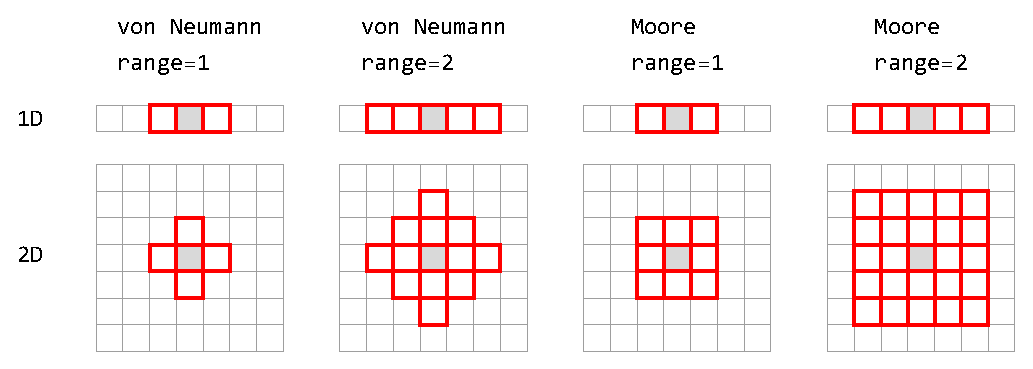
\includegraphics[scale=.8]{ca7} 
\caption{The concept of range in 1D and 2D cellular automatons and how it is defined according to von Neumann and Moore neighbourhoods. With basis in the grey cell, the red lines indicate the neighbours at range one and two in the two dimensions and for the two types of neighbourhoods.\\}
\label{fig:CArange}
\end{figure}

Let us stick to simple rules but now we introduce a state continuum, replacing the discrete states of black, white or other cells. A continuum could be represented by all real numbers between zero and one. This gives an infinite number of possible states in the cell. This class of cellular automatons are labelled continuous cellular automata, referring to the state variable while the time variable is discrete by definition in cellular automata.

\begin{theorem}[Continuous Cellular Automata (CCA)]
\hfill \break
%\mmaCellGraphics[form=TraditionalForm]{Output}{pg1.pdf}
Continuing from code box~\ref{code:cellularautomata} (building on Eide (2012)\cite{Eide2012})

Now we set up a simple 1D (one dimension or linear distribution model) CCA model with range $= 1$ which in our example means that the biomass in one cell is equally distributed into the cell in question and its two neighbouring cells the next time period. This is obtained by the function
\index{\texttt{Map}}\index{\texttt{Sum}}\index{\texttt{RotateLeft}}\index{\texttt{RotateRight}}
\begin{mmaCell}[index=9]{Input}
  CCAEvolveStep[growth_, list_List, range_] := 
    Map[growth, 
      (Sum[RotateLeft[list, i], \{i, range\}] + list + 
      Sum[RotateRight[list, i], \{i, range\}])/(2 range + 1)
    ]
\end{mmaCell}
Let us test how the function works when using the initial world from input 1 in code box~\ref{code:cellularautomata} (also here we consider the two terminal cells to be neighbours, indicating a circular world):
\begin{mmaCell}{Input}
  CCAEvolveStep[growth, world, 1]
\end{mmaCell}
\begin{mmaCell}{Output}
  \{growth\Big[\mmaFrac{1}{3}\Big], growth\Big[\mmaFrac{2}{3}\Big], growth\Big[\mmaFrac{1}{3}\Big], growth\Big[\mmaFrac{1}{3}\Big], growth\Big[\mmaFrac{1}{3}\Big], 
  growth\Big[\mmaFrac{2}{3}\Big], growth[1], growth[1], growth\Big[\mmaFrac{2}{3}\Big], growth\Big[\mmaFrac{2}{3}\Big]\}
\end{mmaCell}
As we have not yet defined the growth function, only the arguments in the unknown growth function are calculated. These arguments gives the total cell biomass after distributing all the initial cell biomasses according to the rule.

A repeated version of \texttt{CCAEvolveStep} is obtained by using the \texttt{NestList} command in \textit{Mathematica}:
\index{\texttt{NestList}}
\begin{mmaCell}{Input}
  CCAEvolveList[growth_, list_List, range_, t_Integer] := 
  NestList[CCAEvolveStep[growth, #, range]&, list, t]
\end{mmaCell}
Assume linear growth in the biomass within each cell with a growth rate of 50\%. If the biomass in one cell passes the value 1.0 the fractional value represents the surviving biomass. With this growth function the world will develop like this the next five periods:
\index{\texttt{ArrayPlot}}\index{\texttt{FractionalPart}}
\begin{mmaCell}{Input}
  ArrayPlot[
    CCAEvolveList[FractionalPart[# 3/2]&, world, 1, 5], 
    Mesh -> True
  ]
\end{mmaCell}
\begin{mmaCell}[moregraphics={moreig={scale=.5}}]{Output}
  \mmaGraphics{ca9}
\end{mmaCell}
Let us stick to the distributional rule and biological growth presented above and increase the number of cells from 10 to 500, using w0 from input 7 in code box~\ref{code:cellularautomata}. Summing up the total biomass of the 500 cells each period gives this plot:
\index{\texttt{ListLinePlot}}\index{\texttt{Total}}\index{\texttt{FractionalPart}}
\begin{mmaCell}{Input}
  ListLinePlot[
    Total /@ CCAEvolveList[FractionalPart[# 3/2]&, w0, 1, 100], 
    AxesLabel -> \{"Period", "Biomass"\}
  ]
\end{mmaCell}
\begin{mmaCell}[moregraphics={moreig={scale=.7}}]{Output}
  \mmaGraphics{ca8}
\end{mmaCell}
The growth curve above looks like a noisy version of the growth curves we found in code boxes~\ref{code:gompertz},~\ref{code:verhulst} and~\ref{code:cohortbiomass}. The growth curve will describe different path towards the equilibrium level of 250 (half of the 500 cells) when changing the distribution of the initial ten cells filled up with biomasses.
\label{code:CCA}
\end{theorem}

Let us now introduce 2D models. If we have a lattice of cells as shown in figure~\ref{fig:CArange} it may represent a graphical area in which fish is distributed in patterns according to predefined rules and different characteristics of the cells. So far we have assumed homogeneous cells but they may have different growth properties which in its simplest form could be implemented by differences in the cells carrying capacities.

In code box~\ref{code:2D CA} the basic principles of 2D cellular automata are introduced.

\begin{theorem}[2D cellular automata modelling]
\hfill \break
%\mmaCellGraphics[form=TraditionalForm]{Output}{pg1.pdf}
Let us start by making a 10 times 10 matrix where 0 and 1 are randomly distributed on the different cells. We call the matrix ocean:
\index{\texttt{Table}}\index{\texttt{RandomInteger}}
\begin{mmaCell}[index=1]{Input}
  ocean = Table[RandomInteger[1, 10], \{10\}]
\end{mmaCell}
\begin{mmaCell}{Output}
  \{\{1, 1, 0, 0, 1, 1, 1, 0, 0, 1\}, \{0, 1, 0, 0, 0, 1, 0, 0, 1, 1\}, 
  \{0, 1, 0, 1, 1, 0, 0, 1, 0, 1\}, \{1, 1, 0, 1, 1, 1, 1, 0, 1, 1\}, 
  \{1, 0, 1, 0, 0, 1, 0, 0, 0, 1\}, \{1, 1, 0, 0, 0, 1, 0, 0, 1, 1\}, 
  \{0, 0, 1, 1, 0, 0, 0, 1, 0, 1\}, \{0, 0, 0, 0, 0, 0, 1, 0, 0, 1\}, 
  \{1, 1, 0, 1, 1, 0, 1, 1, 1, 1\}, \{1, 0, 1, 1, 0, 1, 0, 1, 0, 1\}\}
\end{mmaCell}
In order to implement a rule based on Moore neighbourhood with range 1 (see figure~\ref{fig:CArange}) we need to express the rule in a 3 times 3 matrix. Let the rule be to uniformly distribute the cell content into the nine cells. The the rule is\index{\texttt{Table}}
\begin{mmaCell}{Input}
  rule = Table[1, \{3\}, \{3\}] / 9
\end{mmaCell}
\begin{mmaCell}{Output}
  \Big\{\Big\{\Big[\mmaFrac{1}{9}\Big], \Big[\mmaFrac{1}{9}\Big], \Big[\mmaFrac{1}{9}\Big]\Big\}, \Big\{\Big[\mmaFrac{1}{9}\Big], \Big[\mmaFrac{1}{9}\Big], \Big[\mmaFrac{1}{9}\Big]\Big\}, \Big\{\Big[\mmaFrac{1}{9}\Big], \Big[\mmaFrac{1}{9}\Big], \Big[\mmaFrac{1}{9}\Big]\Big\}\Big\}
\end{mmaCell}
\index{\texttt{ArrayPlot}}\index{\texttt{ListConvolve}}
\begin{mmaCell}{Input}
  ArrayPlot[#, Mesh -> True]& /@ \{
    ocean, ListConvolve[rule, ocean, 1, 0]\}
\end{mmaCell}
\begin{mmaCell}[moregraphics={moreig={scale=.5}}]{Output}
  \mmaGraphics{ca10}
\end{mmaCell}
The three arguments
\index{\texttt{N} (Numeric)}\index{\texttt{GraphicsRow}}\index{\texttt{Total}}\index{\texttt{Flatten}}\index{\texttt{ToString}}\index{\texttt{ArrayPlot}}\index{\texttt{NestList}}\index{\texttt{ListConvolve}}
\begin{mmaCell}{Input}
  GraphicsRow[
    ArrayPlot[#, 
      Mesh -> True, 
      ColorFunction -> "Rainbow",
      PlotLabel -> "Total = "<>ToString @ N @ Total @ Flatten[#],
      PlotRange -> \{0, 1\}
    ] & /@ NestList[ListConvolve[rule, #, 1] &, ocean, 4]
  ]
\end{mmaCell}
\begin{mmaCell}[moregraphics={moreig={scale=.6}}]{Output}
  \mmaGraphics{ca11}
\end{mmaCell}
In all the five development steps above one gets 52 when summarising the content of all cells. The content of the initial 52 filled cells has been redistributed according to the rule when assuming the bottom row to be neighbour of the top row and the left column to be neighbour with the right column. This remains independent of how many development steps included, as for example after 100 steps:
\index{\texttt{Total}}\index{\texttt{ListConvolve}}\index{\texttt{Flatten}}\index{\texttt{Nest}}
\begin{mmaCell}{Input}
  Nest[ListConvolve[rule,#,1]&,ocean,100] //Flatten //Total //N
\end{mmaCell}
\begin{mmaCell}{Output}
  52.
\end{mmaCell}
By adding an argument in the \texttt{ListConvolve} command the boarder neighbourhoods are fixed to the given argument, as in this case are empty cells (0):
\index{\texttt{GraphicsRow}}\index{\texttt{Total}}\index{\texttt{Flatten}}\index{\texttt{ToString}}\index{\texttt{ArrayPlot}}\index{\texttt{NestList}}\index{\texttt{ListConvolve}}
\begin{mmaCell}{Input}
  GraphicsRow[
    ArrayPlot[#, 
      Mesh      -> True, 
      ColorFunction -> "Rainbow",
      PlotLabel -> "Total = "<>ToString @ N @ Total @ Flatten[#],
      PlotRange -> \{0, 1\}
    ] & /@ NestList[ListConvolve[rule, #, 1, 0] &, ocean, 4]
  ]
\end{mmaCell}
\begin{mmaCell}[moregraphics={moreig={scale=.6}}]{Output}
  \mmaGraphics{ca12}
\end{mmaCell}
Surrounded by empty cells and letting the content of the 100 cells (where initially 52 cells are filled) diffuse into the infinite number of surrounding cells, after some time all cells become empty:
\index{\texttt{Nest}}\index{\texttt{ListConvolve}}\index{\texttt{Flatten}}\index{\texttt{Total}}\index{\texttt{Chop}}\index{\texttt{N} (Numeric)}
\begin{mmaCell}{Input}
  Nest[ListConvolve[rule, #, 1, 0] &, ocean, 100
  ] // Flatten // Total // N // Chop
\end{mmaCell}
\begin{mmaCell}{Output}
  0
\end{mmaCell}
In the case below, the surrounding cells are half filled (1/2) and after some time all cells become 50\% filled:  
\index{\texttt{GraphicsRow}}\index{\texttt{Total}}\index{\texttt{Flatten}}\index{\texttt{ToString}}\index{\texttt{ArrayPlot}}\index{\texttt{NestList}}\index{\texttt{ListConvolve}}
\begin{mmaCell}{Input}
  GraphicsRow[
    ArrayPlot[#, 
      Mesh      -> True, 
      ColorFunction -> "Rainbow",
      PlotLabel -> "Total = "<>ToString@N@Total@Flatten[#],
      PlotRange -> \{0, 1\}
    ] & /@ NestList[ListConvolve[rule, #, 1, 1/2]&, ocean, 4]
  ]
\end{mmaCell}
\begin{mmaCell}[moregraphics={moreig={scale=.6}}]{Output}
  \mmaGraphics{ca13}
\end{mmaCell}
\index{\texttt{Total}}\index{\texttt{Flatten}}\index{\texttt{ToString}}\index{\texttt{Nest}}\index{\texttt{N} (Numeric)}\index{\texttt{ListConvolve}}
\begin{mmaCell}{Input}
  Nest[ListConvolve[rule,#,1,1/2]&,ocean,100]//Flatten//Total//N
\end{mmaCell}
\begin{mmaCell}{Output}
  50.
\end{mmaCell}
The development could be considered as a demonstration of the second law of thermodynamics reflecting increased entropy as the biomass spatially levels out by time. The Shannon Function H\cite{Spellerberg2003} is often employed as a diversity or entropy indicator:
\index{\texttt{Sum}}\index{\texttt{Log}}\index{\texttt{Length}}
\begin{mmaCell}{Input}
  shannonH[l_List] := -Sum[l[[i]]*Log[l[[i]]], \{i, Length[l]\}]
\end{mmaCell}
Since
\index{\texttt{Limit}}\index{\texttt{Log}}
\begin{mmaCell}{Input}
  Limit[x * Log[x], x -> 0]
\end{mmaCell}
\begin{mmaCell}{Output}
  0
\end{mmaCell}
and to accommodate lists which sum up to different totals we improve the code of Function H
\index{\texttt{Module}}\index{\texttt{Select}}\index{\texttt{Log}}\index{\texttt{Sum}}\index{\texttt{Length}}\index{\texttt{Total}}
\begin{mmaCell}{Input}
  shannonH[l_List] := 
    Module[\{nl = Select[l/Total[l], # > 0 &]\},
      - Sum[nl[[i]] * Log[nl[[i]]], \{i, Length[nl]\}]
    ]
\end{mmaCell}
where \texttt{nl} is the list normalised to sum up to one. The \texttt{shannonH} function then becomes a diversity indicator which reflects the distribution of biomasses on the different cells. Low index values indicate scattered distribution while high values indicate homogeneous distribution patterns (high diversity). In our case this is exemplified by the initial distribution (\texttt{ocean}) and equal biomass in all cells (indicated by \texttt{x} below):
\index{\texttt{Flatten}}
\begin{mmaCell}{Input}
  shannonH[Flatten@ocean]
\end{mmaCell}
\begin{mmaCell}{Output}
  Log[52]
\end{mmaCell}
\index{\texttt{Table}}
\begin{mmaCell}{Input}
  shannonH[Table[x, {100}]]
\end{mmaCell}
\index{\texttt{Log}}
\begin{mmaCell}{Output}
  Log[100]
\end{mmaCell}
\label{code:2D CA}
\end{theorem}

%------------------------------------------------
\section{Stage structured models}

In stage structured models the population is separated into different fractions based on age or other measures of development (stages). INTRODUCTION TO STAGE MODELS WITHOUT THE USE OF LINEAR ALGEBRA.

A common method of presenting such information is by the use of the Leslie matrix\cite{Leslie1945} where the first line of a matrix gives the breeding numbers ($b$) produced at different stages. The following lines of the square matrix display the survival rates between stages, or the probability of surviving from stage $i$ to stage $i+1$ ($p_{i}$). The survival rates most probabilities becomes zero the Leslie matrix simplifies to
\begin{equation}
\label{eq:lesliem}
L = 
\begin{bmatrix}
    b_{0} & b_{1} & \dots  & b_{m-1}  & b_{m} \\
    p_{0}  & 0 & \dots  & 0 & 0 \\
    0  &  p_{1} & \dots  & 0 & 0 \\
    \vdots  & \vdots & \ddots & \vdots & \vdots \\
    0  & 0 & \dots  & p_{m-1} & 0
\end{bmatrix}
\end{equation}
when separating the population into $m$ stages.

Assume the initial state (at time $t$) of the population in terms of number of individuals of each stage to be given by the vector $\vec{N}_t$,
\begin{equation}
\vec{N}_{t} = 
\begin{bmatrix}
    n_{0,t} \\
    n_{1,t} \\
    n_{2,t} \\
    \vdots \\
    n_{m,t}
\end{bmatrix}
\end{equation}
Then the numbers of individuals at time $t+1$ are given by
\begin{equation*}
 \vec{N}_{t+1} = L \bullet \vec{N}_{t}
\end{equation*}
or the more general form when the initial population is given at time zero:
\begin{equation}
 \vec{N}_{t} = L^t \bullet \vec{N}_{0}
\end{equation}
A numerical example is shown in code box~\ref{code:leslie}, where also it is shown how the equilibrium population is obtained by utilising the properties of the matrix eigenvector.
\begin{theorem}[The Leslie Matrix Model]
\hfill \break
Defining a general $(m+1) \times (m+1)$ Leslie matrix:
\index{\texttt{Range}}\index{\texttt{Table}}\index{\texttt{Prepend}}
\begin{mmaCell}[index=1]{Input}
   leslie[m_] := 
    Prepend[
      Table[
        If[i != j, 0, p[i]],
        \{i, 0, m - 1\}, \{j, 0, m\}
      ],
      b /@ Range[0, m]
    ]
\end{mmaCell}
A $4 \times 4$ Leslie matrix could then for example be obtained:
\index{\texttt{MatrixForm}}
\begin{mmaCell}{Input}
  leslie[3] // MatrixForm
\end{mmaCell}
\begin{mmaCell}[form=MatrixForm]{Output}

\end{mmaCell}
   $ \begin{pmatrix}
  b(0) & b(1) & b(2) & b(3) \\
  p(0) & 0 & 0 & 0 \\
  0 & p(1) & 0 & 0 \\
  0 & 0 & p(2) & 0 \\
  \end{pmatrix} $
  
Assume that the first stage of a $4 \times 4$ Leslie matrix model covers \textit{juveniles}, followed by \textit{young adults}, \textit{adults} and \textit{old adults}. A numerical example is provided by the Leslie matrix \texttt{vleslie}:
\begin{mmaCell}{Input}
  vleslie = 
    leslie[3] /. \{
      b[0] -> 0, b[1] -> .6, b[2] -> 1, b[3] -> 2, 
      p[0] -> .5, p[1] -> .7, p[2] -> .5\}
\end{mmaCell}
\begin{mmaCell}{Output}
  \{\{0, 0.6, 1, 2\}, \{0.5, 0, 0, 0\}, \{0, 0.7, 0, 0\}, \{0, 0, 0.5, 0\}\}
\end{mmaCell}
where the first line gives the fecundity (birth rate) of the four stages (starting to the left with the \textit{juveniles}) and the next rows display the survival rates of the first three 
The equilibrium solution of the model is embedded in the eigenvector of the Leslie matrix. We label it \texttt{eigenvector}:
\index{\texttt{Eigenvectors}}\index{\texttt{Chop}}
\begin{mmaCell}{Input}
  eigenvector = Eigenvectors[vleslie][[1]] // Chop
\end{mmaCell}
\begin{mmaCell}{Output}
  \{0.844213, 0.422106, 0.295474, 0.147737\}
\end{mmaCell}
The percentage distribution of the four stages in equilibrium is given by
\index{\texttt{Total}}
\begin{mmaCell}{Input}
  eigenvector = eigenvector/Total@eigenvector
\end{mmaCell}
\begin{mmaCell}{Output}
  \{0.493827, 0.246914, 0.17284, 0.0864198\}
\end{mmaCell}
The time series of number of individuals of each of the four stages over a period of 15 time units, starting with an initial population where we have 1 \textit{juvenile}, 25 \textit{young adults}, 10 \textit{adults} and 6 \textit{old adults}:
\index{\texttt{Range}}\index{\texttt{MatrixPower}}
\begin{mmaCell}{Input}
  ndevelopment = 
    MatrixPower[vleslie, #].\{1, 25, 10, 6\} & /@ Range[0, 15];
\end{mmaCell}
Then we find the relative distribution of individuals on the four stages over the time period:
\begin{mmaCell}{Input}
  relndevelopment = #/Total@# & /@ ndevelopment;
\end{mmaCell}
which can be viewed as a list plot of the four stages:
\index{\texttt{ListLinePlot}}\index{\texttt{Transpose}}
\begin{mmaCell}{Input}
  ListLinePlot[
    Transpose@relndevelopment,
    PlotRange   -> All, 
    GridLines   -> \{None, eigenvector\}, 
    PlotLegends -> 
      \{"juveniles", "young adults", "adults", "old adults"\},
    AxesLabel   -> \{"Time", "\% of total number"\}
  ]
\end{mmaCell}
\begin{mmaCell}[moregraphics={moreig={scale=.9}}]{Output}
  \mmaGraphics{leslie}
\end{mmaCell}
The equilibrium values (\texttt{eigenvector}) are indicated as horizontal grid lines in the plot.
\label{code:leslie}
\end{theorem}

\begin{figure}[!htb]
\begin{remark}
\rule{\linewidth}{.1pt}
\floatbox[{\capbeside\thisfloatsetup{capbesideposition={right,top},capbesidewidth=11.8cm}}]{figure}[\FBwidth]
{\caption*{\footnotesize{The Leslie matrix can be explored as a \\ Wolfram Demonstration at

\href{http://demonstrations.wolfram.com/AgeDistributionsFromALeslieModelForAgeStructuredPopulations/}{\\ http://demonstrations.wolfram.com/\\AgeDistributionsFromALeslieModelForAgeStructuredPopulations}}}}
{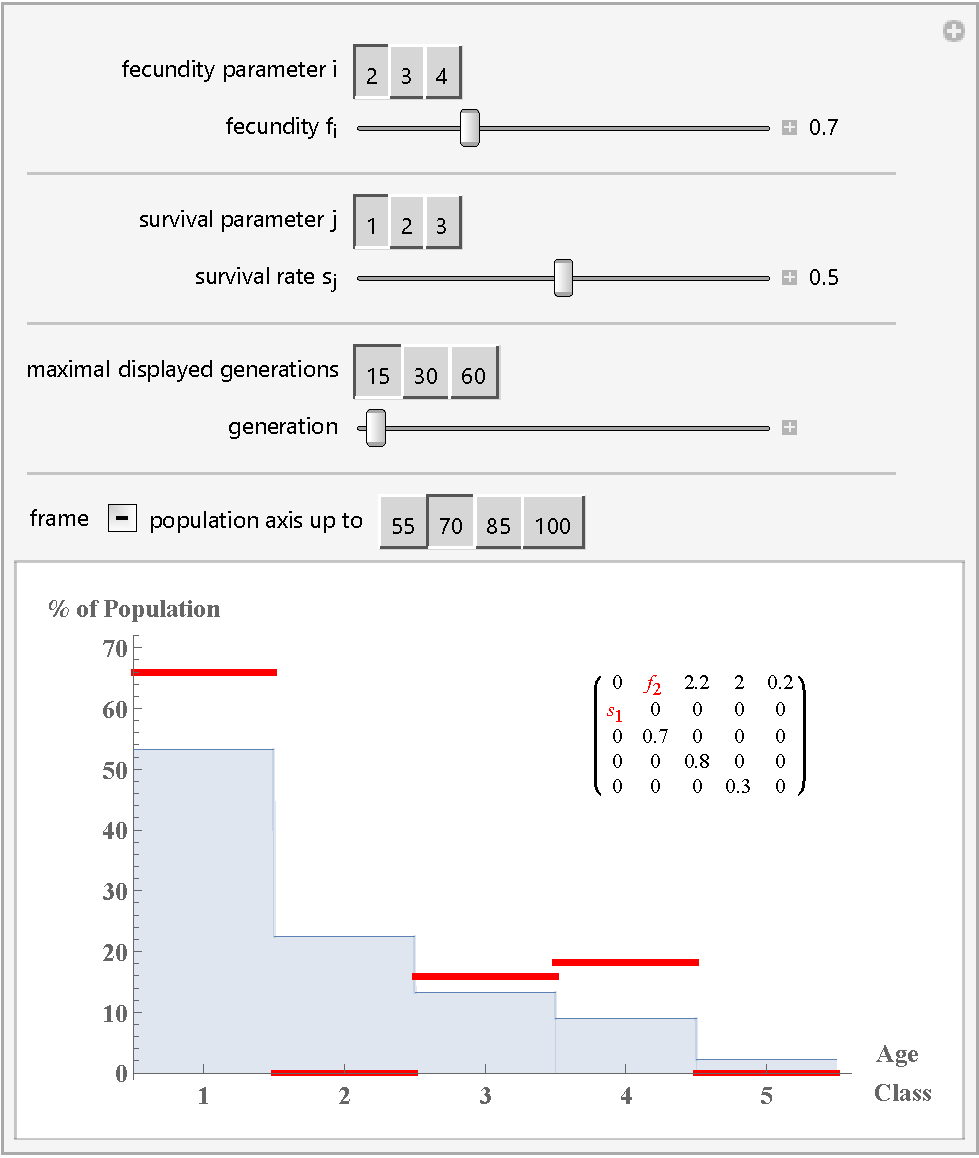
\includegraphics[width=2.8cm]{demo_LeslieMatrix}}\\
\rule[10pt]{\linewidth}{.1pt}\end{remark}\end{figure}

%------------------------------------------------
\section{Multispecies models}\label{section:multispecies}
In the previous sections we have investigated different ways to model population growth of one fish stock and in the next chapter we will add a harvest model to find the net growth in the stock per unit of time. Adding a harvest model to the population dynamics of the fish stock is in principle the same as adding the impact of predation, the humans being the predators in this case. Introducing multispecies modelling here therefore is in a way introducing the exploitation of a fish stock resource in advance of chapter~\ref{chapter 5}.

As indicated by the name multispecies models includes more than one species. Normally this does not include the humans exploitation of fish stock resources but if we should we are definitely talking about a prey-predator relationship. In principle we have three types of multispecies relationships:
\begin{itemize}
\item Prey-predator relations
\item Competing species
\item Symbiotic relationships (which in principle also may include cannibalism)
\end{itemize}
\hfill \break
\index{Multispecies modelling}\index{Multispecies modelling!Lotka-Volterra}One famous prey-predator model is the Lotka-Volterra model named after Alfred Lotka and Vito Volterra\cite{Volterra1938} who independently of each others suggested the model formulation in 1925-1926. Let $x$ be the prey stock biomass, $y$ the predator stock biomass, $a, b, c$ and $d$ are positive constants, and $t$ is the time variable.Then the model formulation
\begin{equation}
\label{eq:lotkavolterra}
\begin{aligned} & \dot{x}(t) = x(t) \cdot \Big(a - b \cdot y(t)\Big) \\
& \dot{y}(t) = - y(t) \cdot \Big(c - d \cdot x(t)\Big)
\end{aligned}
\end{equation}
gives the population growth per unit of time for the prey and for the predator as functions of $x$ and $y$.

The Lotka-Volterra model has a stable focus at $x = c/d$ and $y = a/b$. As seen in Code box~\ref{code:lotkavolterra}, however, the stable focus (the intersection between the two red isoclines\index{Isocline} in the phaseplot\index{Phaseplot} in \texttt{Out[2]}) is the focus of limit cycles which paths are determined by the initial values of $x$ and $y$.

Although the practical use of the Lotka-Volterra model is severely constrained by its sensitivity to the initial condition of the system, the limit cycle property of the model (see Code box~\ref{code:lotkavolterra}) provides an elegant and straightforward illustration of a typical prey-predator relationship. The cycles (see \texttt{Out[3]} in Code box~\ref{code:lotkavolterra}) show how a large prey stock (blue curve) gives room for growth in the predator stock (yellow curve). At some point the increasing predator stock's consumption of the prey stock leads to a decline in the prey stock biomass. Later follows a corresponding decline in the predator stock biomass, which \textendash \space at some point in time \textendash \space again gives room for the prey stock to increase its biomass after which the whole cycle is repeated.

\begin{theorem}[The Lotka-Volterra Model]
\hfill \break
Assume $a = b = c = d = 1$ in Equation~\ref{eq:lotkavolterra} and assume an initial predator biomass $x(0) = 0.5$ while the initial prey biomass ($y(t)$) is given three different values, $0.05$, $0.3$ and $1$. The two differential equations (Equations~\ref{eq:lotkavolterra}) are solved numerically by employing the \texttt{NDSolve} function. We define a function (\texttt{dsol}) in which the initial value of $y$ is a variable:
\index{\texttt{NDSolve}}
\begin{mmaCell}[index=1]{Input}
  dsol[y0_] := 
    NDSolve[\{
      x'[t] == x[t] (1-y[t]), 
      y'[t] == -y[t] (1-x[t]), 
      x[0 ] == .5, 
      y[0]  == y0\},
      \{x[t], y[t]\}, \{t, 0, 25\}
    ];
\end{mmaCell}
Then we use the \texttt{dsol} function to draw the paths of $x-y$\textendash dynamics for three different initial values of $y$. The isoclines of the system are drawn as red lines. The three initial points \textendash \space ($0.5$, $0.05$), ($0.5$, $0.3$) and ($0.5$, $1.0$) \textendash \space are shown as black points in the plot below. The \texttt{VectorPlot} function indicates the directions and varying strength in the dynamics of the system.
\index{\texttt{Show}}\index{\texttt{Graphics}}\index{\texttt{ParametricPlot}}\index{\texttt{Evaluate}}\index{\texttt{VectorPlot}}\index{\texttt{Line}}\index{\texttt{Point}}
\begin{mmaCell}{Input}
  Show[\{
    ParametricPlot[
      Evaluate[\{x[t], y[t]\} /. dsol[#]], \{t, 0, 25\}
    ] & /@ \{.05, .3, 1\}, 
    VectorPlot[\{x(1-y), -y(1-x)\}, 
      \{x, 0, 5\}, \{y, 0, 5\}, 
      VectorScale  -> \{.15, .4, (#1 + #2) &\}, 
      VectorPoints -> 12
    ],
    Graphics[\{
      Red, Line[\{\{1, 0\}, \{1, 5\}\}], Line[\{\{0, 1\}, \{5, 1\}\}],
      Black, PointSize[.025], Point[\{.5, #\}] & /@ \{.05, .3, 1\}
    \}]
  \}]
\end{mmaCell}
\begin{mmaCell}[moregraphics={moreig={scale=.5}}]{Output}
  \mmaGraphics{lotkavolterra1}
\end{mmaCell}
The results may also be presented by the time variable $t$, plotting the changes in $x(t)$ (blue curve) and $y(t)$ (yellow curve) over a period of 25 time steps:
\index{\texttt{Plot}}\index{\texttt{GraphicsRow}}\index{\texttt{Evaluate}}\index{\texttt{ToString}}
\begin{mmaCell}{Input}
  GraphicsRow[
    Plot[Evaluate[\{x[t], y[t]\} /. dsol[#]], \{t, 0, 25\},
      PlotRange -> \{0, 5\}, 
      PlotLabel -> "x(t) = .5, y(t) = " <> ToString[#]
    ] & /@ \{.05, .3, 1\}
  ]
\end{mmaCell}
\begin{mmaCell}[moregraphics={moreig={scale=.5}}]{Output}
  \mmaGraphics{lotkavolterra2}
\end{mmaCell}
Again: The initial conditions determines the fluctuations in terms of wavelengths and frequencies.
\label{code:lotkavolterra}
\end{theorem}
\hfill \break
\index{Multispecies modelling!Prey-Predator}There are many other ways than the Lotka-Volterra model to formulate a prey-predator relation. As mentioned in the introductory part of this section, a fishery is similar to a prey-predator situation. Assume a prey stock which in absence of the predator stock has a population growth as expressed in Equation~\ref{eq:verhulst}. The presence of a predator adds a negative term to the equation and we assume that this negative term is linear in the biomass of both prey and predator. Further assume that the prey is essential for the predator and that the environmental carrying capacity of the predator is linear in the prey stock biomass. This gives the prey-predator model
\begin{equation}
\label{eq:preypredator}
\begin{aligned} & \dot{x}(t) = r \cdot x(t) \cdot \bigg(1 - \frac{x(t)}{K}\bigg) - \alpha \cdot x(t) \cdot y(t)\\
& \dot{y}(t) = s \cdot y(t) \cdot \bigg(1 - \frac{y(t)}{\beta \cdot x(t)}\bigg)
\end{aligned}
\end{equation}
where $r$ and $s$ are the intrinsic growth rates of respectively the prey and the predator stocks while $\alpha$ and $\beta$ are positive constants, $\alpha$ representing a catchability coefficient for the predator harvesting the prey and $\beta$ a measure of the positive impact prey availability has on the population growth in the predator stock. The dynamics of Equations~\ref{eq:preypredator} is illustrated in Figure~\ref{fig:preypredator}. \index{Isocline}Note in particular how the isoclines of the system differ from the isoclines of the Lotka-Volterra model in Code box~\ref{code:lotkavolterra}.
\begin{figure}[ht]
\centering
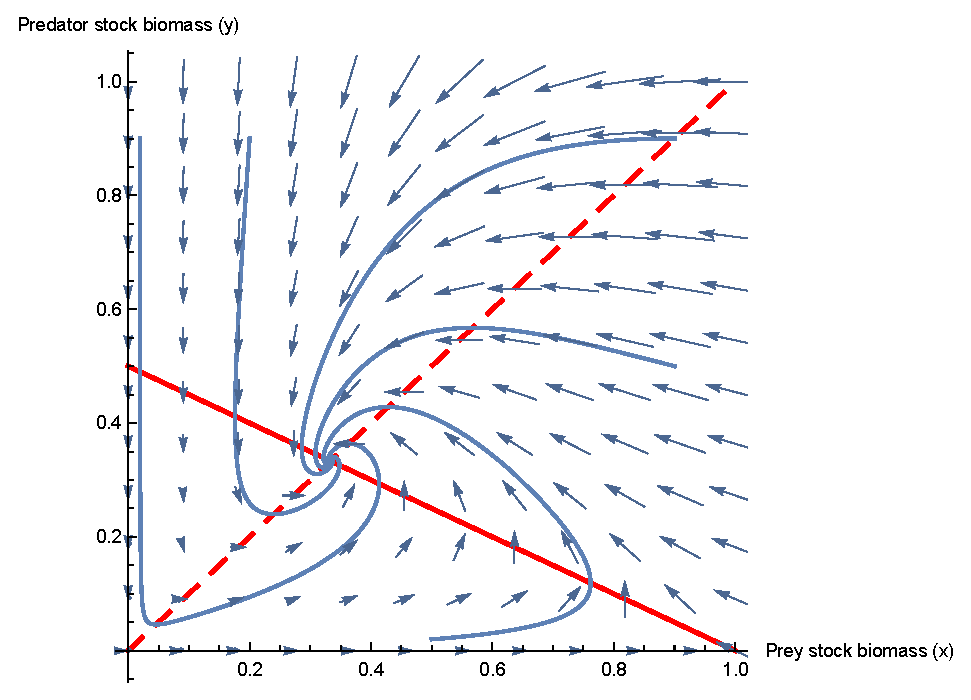
\includegraphics[scale=.8]{preypredator}
\caption{Phaseplot of the prey-predator model in Equations~\ref{eq:preypredator} where $r = s = 0.5$ and $K = \alpha = \beta = 1$. The solid red line is the prey isocline $ \dot{x}(t) = 0$ while the dashed red line is the predator isocline $ \dot{y}(t) = 0$. Five paths towards the stable equilibrium (the intersection between the two isoclines) are shown from five different initial conditions of the system.}
\label{fig:preypredator}
\end{figure}

\index{Multispecies modelling!Competition}While the prey species is negatively impact by the predator and the predator takes advantage of the prey in a prey-predator relationship, all species are negatively affected of each other in a competitive relationship. The famous Russian biologist Georgy Gause formulated (in line with works of Lotka and Volterra) this model of two competing species\cite{Gause1935}:
\begin{equation}
\label{eq:competing}
\begin{aligned} & \dot{x}(t) = r \cdot x(t) \cdot \bigg(1 - \frac{x(t)}{K}\bigg) - \alpha \cdot x(t) \cdot y(t) \\
& \dot{y}(t) = s \cdot y(t) \cdot \bigg(1 - \frac{y(t)}{L}\bigg) - \beta \cdot x(t) \cdot y(t)
\end{aligned}
\end{equation}
where $r$ and $s$ are the intrinsic growth rates of the two competing species. $\alpha$, $\beta$, $K$ and $L$ are positive constants, the two latter representing the environmental carrying capacities of the two species. It is easy to observe that the first equations in the two Systems~\ref{eq:preypredator} and \ref{eq:competing} are identical to each other and that the second equation in System~\ref{eq:competing} is following the same pattern as the first equations.

\index{Isocline}The isoclines of the competing species model may or may not intersect each other and in the case of intersection it may be as in Figure~\ref{fig:competing} where the $\dot{y}(t)=0$ isocline intersects the vertical axis above the $\dot{x}(t)=0$ isocline (the normal case). In this case the intersection between the two isoclines is an unstable equilibrium point. In the opposite case (when the $\dot{x}(t)=0$ isocline intersects the vertical axis above the $\dot{y}(t)=0$ isocline) the intersection between the two isoclines will be a stable equilibrium. According to Gause the latter only occurs if the two species belong to different ecological niches\cite{Gause1935} and hence not are competing species at the same ecological niche. The competitive exclusion principles implies that the two competing species could not coexist, one always will be totally dominating the ecological niche in which they are placed. Therefore there exists two stable equilibriums in the model (as seen in Figure~\ref{fig:competing}), one excluding $x$ and the other excluding $y$.

\begin{figure}[ht]
\centering
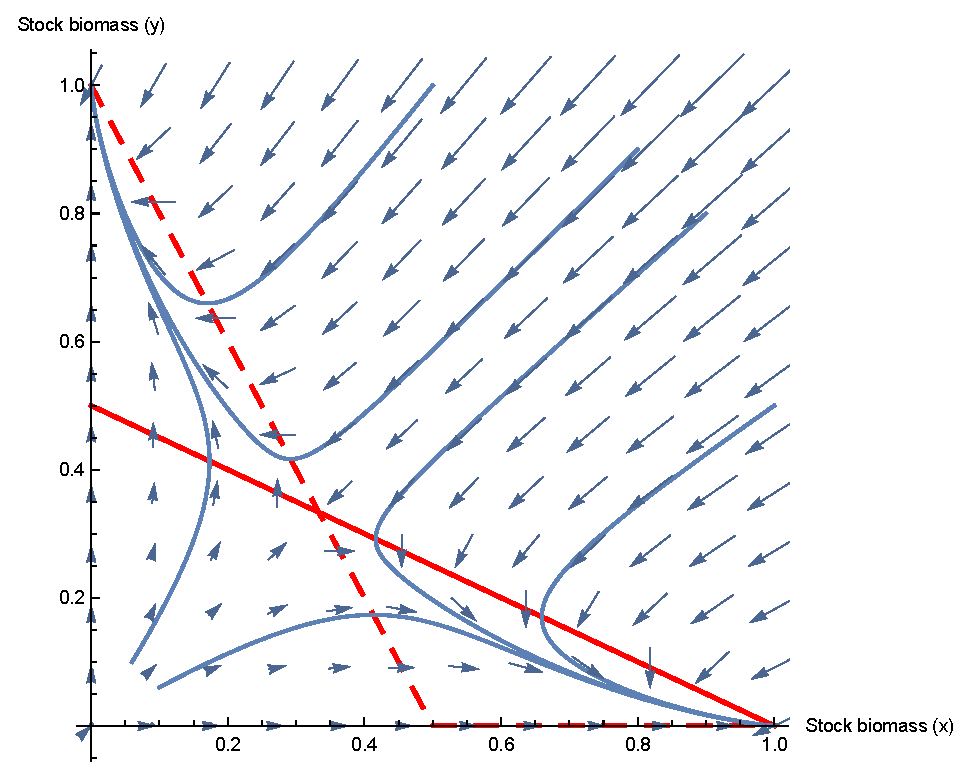
\includegraphics[scale=.7]{competing}
\caption{Phaseplot of the competition model in Equations~\ref{eq:competing} where $r = s = 0.5$ and $K = L = \alpha = \beta = 1$. The solid red line is the isocline $ \dot{x}(t) = 0$ while the dashed red line is the isocline $ \dot{y}(t) = 0$. Six paths towards the two stable equilibriums (in point (1,0) and point (0,1)) are shown from five different initial conditions of the system. The intersection between the two isoclines is an unstable equilibrium point.}
\label{fig:competing}
\end{figure}

\index{Multispecies modelling!Symbiosis}Symbiosis, the opposite of competition, is also a possible relationship between two or more species. A very simple symbiosis model is
\begin{equation}
\label{eq:symbiosis}
\begin{aligned} & \dot{x}(t) = r \cdot x(t) \cdot \bigg(1 - \frac{x(t)}{K + \alpha \cdot y(t)}\bigg) \\
& \dot{y}(t) = s \cdot y(t) \cdot \bigg(1 - \frac{y(t)}{L + \beta \cdot x(t)}\bigg)
\end{aligned}
\end{equation}
\index{Isocline}where $r$ and $s$ as in Equations~\ref{eq:preypredator} and \ref{eq:competing} represent the intrinsic growth rates of the two species. Here the environmental carrying capacities of $x$ and $y$ are $K + \alpha \cdot y$ and $L + \beta \cdot x$, respectively. Symbiosis and cannibalism models (as any multspecies model) may also have curved isoclines as for example shown by Eide and Wikan (2010)\cite{Eide2010}.

\begin{figure}[ht]
\centering
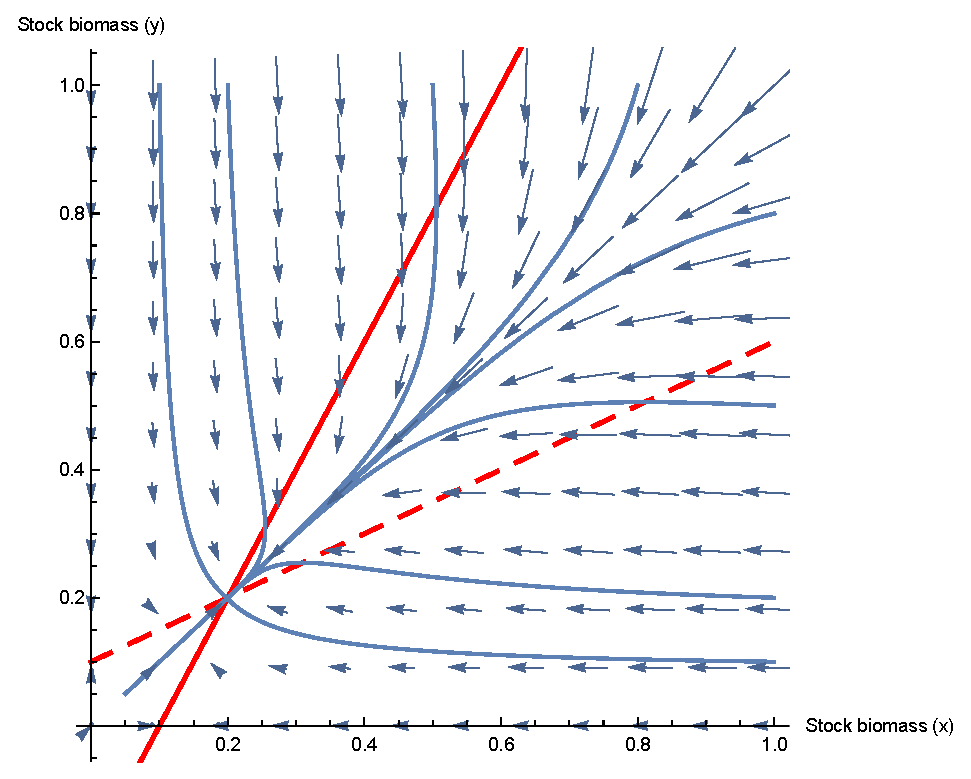
\includegraphics[scale=.7]{symbiosis}
\caption{Phaseplot of the symbiosis model in Equations~\ref{eq:symbiosis} where $r = s = \alpha = \beta =0.5$ and $K = L = 0.1$. The solid red line is the isocline $ \dot{x}(t) = 0$ while the dashed red line is the isocline $ \dot{y}(t) = 0$. Several paths towards the stable equilibrium at the intersection between the two isoclines are shown from different initial conditions of the system.\\}
\label{fig:symbiosis}
\end{figure}

\begin{figure}[!htb]\begin{remark}
\rule{\linewidth}{.1pt}
\floatbox[{\capbeside\thisfloatsetup{capbesideposition={right,top},capbesidewidth=11.8cm}}]{figure}[\FBwidth]
{\caption*{\footnotesize{Explore a three-species model as a Wolfram Demonstration here:

\href{http://demonstrations.wolfram.com/EcosystemDynamics/}{\\ http://demonstrations.wolfram.com/EcosystemDynamics/}}}}
{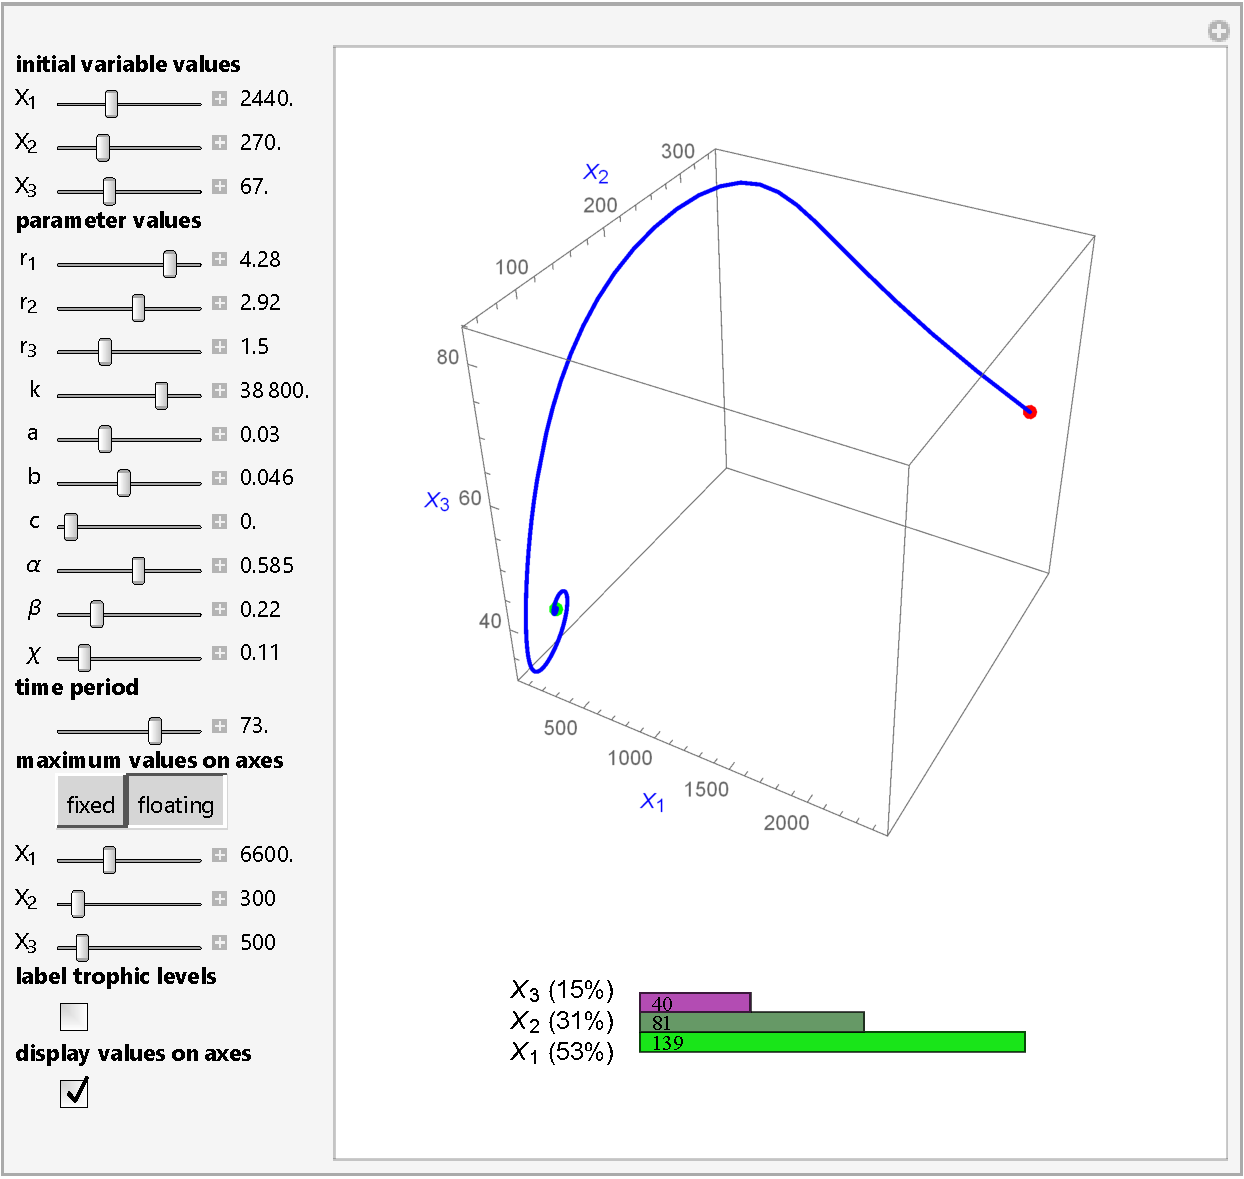
\includegraphics[width=2.8cm]{demo_EcosystemDynamics}}\\
\rule[10pt]{\linewidth}{.1pt}
\end{remark}\end{figure}

%------------------------------------------------
\section{Stock assessment}\label{section:assessment}

Stock assessments are essential procedures in modern fisheries management, as the state of the stock at any point in time is the most important information in this process. In order to sustain a fishery the resource base of this fishery has to be sustained. Hence, the state of the resource base is a core issue.

Stock assessment is however about more than only map the current stock biomass in the sea. While referring to \textit{the state of the stock} in this context it also means the future development of the stock at the current level of exploitation as well as at different levels of exploitation.

The main data sources to perform fish stock assessment are catch statistics, and records from trawl (swept-area method) and acoustic surveys. How time series of catch statistics may be utilised to obtain rough stock estimates is described in code box~\ref{code:cobbdouglas3}. In this example a specific population growth model (logistic growth) is assumed, illustrating the fact that all use of catch data makes use of some predefined assumptions related to models on stock growth and/or harvest production. Obviously this is also the case for swept-area surveys but also acoustic stock assessment surveys involves pre-assumed model on how acoustic signals relate to stock densities. Modern technology therefore does not seem to be able to solve the principal problem described by Slobodkin in Additional remarks~\ref{highlight:slobodkin}.

\begin{corollary}[Is it possible to determine a population's size in nature?]
\hfill \break
\small{\textit{From "Growth and Regulation of Animal Populations" (page 152), by Lawrence B. Slobodkin}\cite{Slobodkin1961}: \\ \indent \enquote{Unfortunately, one of the most difficult things to determine about any animal population is its size in nature. Derivatives of growth curves and details of courting, mating, psychology, and evolution, which would seem fairly abstruse, are relatively simple to determine; but a complete numerical census requires simultaneous observations of the population over a large area and has been made for very few organisms. Consequently, it would seem that the appropriate procedures for testing the reality of oscillations in population numbers in animals would have to be either theoretical -- that is, in terms of biologically realistic models -- or experimental.}
}
\label{highlight:slobodkin}
\end{corollary}

\section*{Exercises}\index{Exercises!Chapter 4}
\addcontentsline{toc}{section}{Exercises}
\begin{exercise}
Modify the WL code in Code box~\ref{code:growth} (Input 4) and  try to reproduce the graphs in Figure~\ref{fig:cobwebharvest}.
\end{exercise}
\begin{exercise}
Show how to calculate the stable focus of the Lotka-Volterra model.
\end{exercise}


\chapterimage{h5.jpg} % Chapter heading image
%------------------------------------------------
\chapter{The concept of equilibrium harvest} \label{chapter 5}
%----------------------------------------------------------------------------------------
%	CHAPTER 5
%----------------------------------------------------------------------------------------
\index{Equilibrium harvest}
The idea of equilibrium harvest is straight forward: Equilibrium harvest is obtained when the surplus biomass production in the stock during a period of time is harvested during the same period. This simplification has however some problems since an equilibrium condition is a highly theoretical concept.

The surplus production is the net production when taking into consideration \textit{recruitment} (in a fishery perspective this is often considered being the young fish when passing the size or age by which they could be captured), \textit{individual growth} which is the total increment in size obtained by all individuals, and \textit{natural mortality} which is the biomass loss due to all the fish dying during the period.

Obviously the harvest production during a period could not be exactly the biomass constituting the surplus production during the same period. It is equally obvious that it does matter how the harvested biomass is put together, if it is newly recruited young fish or older fish.

These are problems which are omitted in the standard surplus production models discussed in section~\ref{section:surplus production}. These models do not take into account the age composition of the stock or how the recruitment dynamics links to this composition. A certain biomass at the beginning of a year gives a certain surplus production in that year. The problems discussed above therefore does not affect the surplus production models. But what about the age structured models presented in section~\ref{section:age structured model}? Is it possible to stick to the idea of equilibrium harvest in the case of age structured models?

The way the equilibrium concept is interpreted in age structured models is through fixed fishing mortality rates for each cohort. The total mortality rate $Z$ is decomposed into natural mortality rate $M$, the mortality that naturally occurs through predation, age and diseases, and $F$, the mortality rate imposed through fishing:
\begin{equation} 
\label{eq:mortality}
Z = M + F
\end{equation}
The harvest obtained from each cohort is then given by the product of the fishing mortality rate for the cohort, $F_c$, and the biomass of the cohort, $X_c$, which is the equilibrium biomass of the cohort after keeping all fishing mortalities constant for a sufficiently long period of time. Hence, equilibrium harvest is also a well defined concept within the tradition of age structured models.

\section{Surplus production models}\index{Surplus production!Equilibrium harvest|textbf}
Net growth per unit of time in the stock biomass is given by the difference between the natural growth of the stock (surplus production $f(X)$) and the harvest ($H(E,X)$): 
\begin{equation} 
\label{eq:stockchange}
\dot{X}(t) = f\big(X(t)\big) - H\big(E(t),X(t)\big)
\end{equation}
When inserting for the surplus productions defined by growth equations~\ref{eq:gompertz},~\ref{eq:verhulst} and~\ref{eq:richards}, the respective expressions of equation~\ref{eq:stockchange} are:
\begin{equation} 
\label{eq:hgompertz}
\dot{X}(t) = - r \cdot X(t) \cdot ln\Big(\frac{X(t)}{K}\Big) - H\big(E(t),X(t)\big)
\end{equation}
\begin{equation}
\label{eq:hverhulst}
\dot{X}(t) = r \cdot X(t) \Big(1 - \frac{X(t)}{K}\Big) - H\big(E(t),X(t)\big)
\end{equation}
\begin{equation}
\label{eq:hrichards}
\dot{X}(t) = r \cdot X(t) \bigg( 1 - \bigg(\frac{X(t)}{K}\bigg)^{m - 1} \bigg) - H\big(E(t),X(t)\big)
\end{equation}
$H(E,X)$ is the harvest obtained throughout the period of one time step (often a year). Assume $H(E,X)$ to be a bi-linear catch equation given by equation~\ref{eq:schaeffer}. While keeping a constant fishing effort, $E(t) = E$, equilibrium is obtained when $\dot{X}(t) = 0$ for all $t$. The stock biomass reaches the equilibrium value $X$, which in the case of equation~\ref{eq:hverhulst} is found through the following steps:
\begin{align*}
r \cdot X \Big(1 - \frac{X}{K}\Big) = q \cdot E \cdot X
\end{align*}
If $X \neq 0$:
\begin{align*}
r \Big(1 - \frac{X}{K}\Big) = q \cdot E,
\end{align*}
which by reorganising the terms gives the equilibrium biomass
\begin{equation}
\label{eq:stockeq}
X = K \Big(1 - \frac{q}{r} E\Big)
\end{equation}

We see that the equilibrium biomass, while assuming a logistic growth equation (the Verhulst equation) and a Schaeffer production function, is a linear function of any value the constant fishing effort $E$ may have.

\begin{theorem}[Equilibrium harvest]
\hfill \break
The linear relationship in equilibrium, between constant fishing effort $E$ and stock biomass $X$, expressed in equation~\ref{eq:stockeq}, is illustrated below for some given parameter values ($K = 1$, $r = 1/2$ and $q = 1/2$):
\index{\texttt{Plot}}\index{\texttt{Solve}}
\begin{mmaCell}[index=1]{Input}
  Plot[
    x /. Solve[r x (1-x/k) == q ee x && x != 0, x] /. \{
      k -> 1, q -> 1/2, r -> 1/2, ee -> e\},
    \{e, 0, 1\},
    PlotStyle -> Red, 
    AxesLabel -> \{"E", "X"\}
  ]
\end{mmaCell}
\begin{mmaCell}[moregraphics={moreig={scale=.6}}]{Output}
  \mmaGraphics{xeq}
\end{mmaCell}
Recall the Cobb-Douglas function plot in Code box~\ref{code:ces} and join a contour plot of the short term catch equation~\ref{eq:schaeffer} with the plot above:
\index{\texttt{Range}}\index{\texttt{Show}}\index{\texttt{ContourPlot}}\index{\texttt{Solve}}
\begin{mmaCell}{Input}
  Show[
    ContourPlot[
      (q e x /. \{k - >1, q - >1/2, r - >1/2\}) == #, 
      \{x, 0, 1\}, \{e, 0, 1\}
    ] & /@ Range[0.01, .6, .04],
    Plot[x /. Solve[r x (1 - x/k) == q ee x && x != 0, x] /. \{
        k - >1, q - >1/2, r - >1/2, ee - >e\}, 
      \{e, 0, 1\}, 
      PlotStyle -> Red
    ], 
    PlotRangePadding -> None, 
    FrameLabel       -> \{"E", "X"\}
  ]
\end{mmaCell}
\begin{mmaCell}[moregraphics={moreig={scale=.6}}]{Output}
  \mmaGraphics{xeq2}
\end{mmaCell}
Imagine the red line in the plot above projected down at the surface of the production equation. Then the red line will describe a curve through the three dimensions of $E$, $X$ and $H$ as in this plot:
\index{\texttt{ParametricPlot3D}}
\begin{mmaCell}{Input}
  ParametricPlot3D[\{e, k (1 - q/r e), q e k (1 - q/r e)\} /. \{
    k -> 1, q -> 1/2, r -> 1/2\}, 
    \{e, 0, 1\}, 
    BoxRatios -> \{1, 1, 1\}, 
    PlotStyle -> Directive[Thickness[.015], Red], 
    AxesLabel -> \{"E", "X", "H"\}
  ]
\end{mmaCell}
\begin{mmaCell}[moregraphics={moreig={scale=.6}}]{Output}
  \mmaGraphics{xeq3}
\end{mmaCell}
We can also use \textit{Mathematica} to view how the long term relationship (the red curve) is placed into the short term catch equation (the surface below):
\index{\texttt{Plot3D}}\index{\texttt{Show}}\index{\texttt{Specularity}}\index{\texttt{ParametricPlot3D}}
\begin{mmaCell}{Input}
  Show[\{
    Plot3D[q e x /. \{k -> 1, q -> 1/2, r -> 1/2\},
      \{x, 0, 1\}, \{e, 0, 1\},
      MeshFunctions -> \{#3 &\}, 
      PlotStyle -> Directive[
        Opacity[0.7], LightBlue, Specularity[White, 50]
      ]
    ],
    ParametricPlot3D[\{e, k (1 - q/r e), q e k (1 - q/r e)\} /. \{
      k - >1, q - >1/2, r -> 1/2\},
      \{e, 0, 1\}, 
      PlotStyle -> Directive[Thickness[.015], Red]
    ]\}, 
    BoxRatios -> \{1, 1, 1\}, 
    AxesLabel -> \{"E", "X", "H"\}, 
    ViewPoint -> \{2.3, -.6, .8\}
  ]
\end{mmaCell}
\begin{mmaCell}[moregraphics={moreig={scale=.6}}]{Output}
  \mmaGraphics{xeq5}
\end{mmaCell}
While viewing the red curve from a view point in front of the $X$-axis (\texttt{ViewPoint -> \{Infinity, 0, 0\}}) we see the left graph below. With a view point in front of the $E$-axis (\texttt{ViewPoint -> \{0, -Infinity, 0\}}) we see the graph to the right below.
\index{\texttt{GoldenRatio}}\index{\texttt{GraphicsRow}}\index{\texttt{ParametricPlot3D}}
\begin{mmaCell}{Input}
  GraphicsRow[
    ParametricPlot3D[\{e, k (1 - q/r e), q e k (1 - q/r e)\} /. \{
      k -> 1, q -> 1/2, r -> 1/2\},
      \{e, 0, 1\}, 
      BoxRatios -> \{1, 1, 1/GoldenRatio\}, 
      PlotStyle -> Red,
      ViewPoint -> #, 
      AxesLabel -> \{"E", "X", "H"\}
    ] & /@ \{\{Infinity, 0, 0\}, \{0, -Infinity, 0\}\},  
    Spacings -> 50
  ]
\end{mmaCell}
\begin{mmaCell}[moregraphics={moreig={scale=.8}}]{Output}
  \mmaGraphics{xeq4}
\end{mmaCell}
\label{code:equilibrium}
\end{theorem}

\index{Isocline}Equation~\ref{eq:stockeq} is the isocline for value zero of differential equation~\ref{eq:hverhulst} ($\dot{X}(t) = 0$). The isocline separates the $E-X$-plane into two sections, one section where the stock biomass increases (below the isocline) and one section where the stock biomass is reduced (above the isocline), see Figure~\ref{fig:isocline}.
\hfill \break
\begin{figure}[ht]
\centering
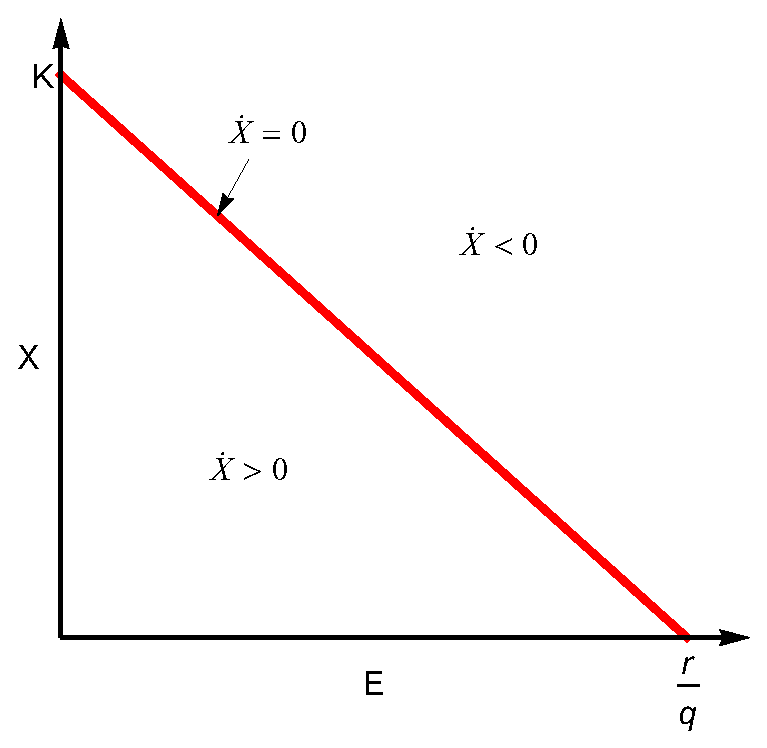
\includegraphics[scale=.6]{isocline}
\caption{The isocline of equation~\ref{eq:hverhulst} is a down-sloping straight line separating the plane into two sections: Below the isocline where the stock biomass increases ($\dot{X}(t) > 0$) and above the line where the stock biomass declines ($\dot{X}(t) < 0$).}
\label{fig:isocline}
\end{figure}
\hfill \break
Figure~\ref{fig:isocline} shows all possible equilibriums as a line while all other combinations of $X$ and $E$ causes increase or decline in the stock biomass $X$. Note that $X = K$ (for $E =0$) and $X = 0$ (for $E =\frac{r}{q}$, see equation~\ref{eq:stockeq}) also are equilibriums, defining the outer boundaries of the isocline.

Having found the equilibrium relationship between fishing effort ($E$) and stock biomass ($X$), equilibrium harvest could be expressed by fishing effort by inserting Equation~\ref{eq:stockeq} into Equation~\ref{eq:schaeffer}:
\begin{equation}
\label{eq:eqharvest}
H(E, X(E)) = H(E) = q K E \Big(1 - \frac{q}{r} E\Big)
\end{equation}
This equation is sometimes referred to the Schaeffer-model due to Schaeffer's first use the model. It should however not be confused with the short term catch equation (Equation~\ref{eq:schaeffer}) which is also valid outside equilibrium.

\label{MSY}\index{Maximum Sustainable Yield (MSY)}Maximum Sustainable Yield ($MSY$) is given by maximising Equation~\ref{eq:eqharvest} with respect of effort ($E$). A maximum is found for $H'(E) = 0$ when $H''(E) < 0$, when $E = r/(2 q)$. Hence, in the case of Equation~\ref{eq:eqharvest}, we have
\begin{equation}
\label{eq:msy}
 MSY = H(E = \frac{r}{2 q}) = \frac{r \cdot K}{4}
\end{equation}

%------------------------------------------------
\section{Stock dynamics in discrete time}
\begin{figure}[ht]
\centering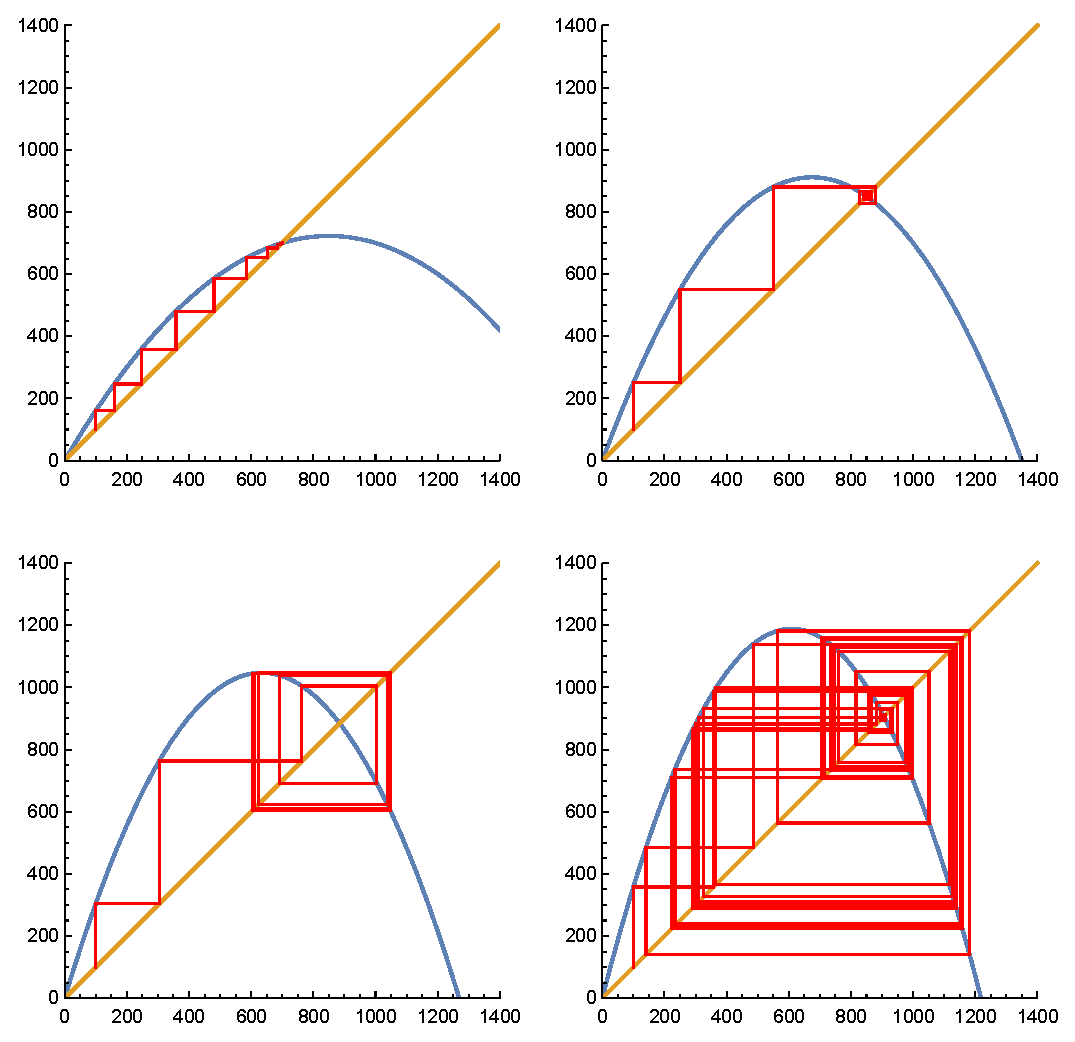
\includegraphics[scale=.7]{harvestdynamics1}
\caption{Cobweb diagram (see Code box~\ref{code:verhulst}) showing how the stock size (at time $t$ along the horizontal axis and at time $t+1$ along the vertical axis) is adjusted according to a fixed fishing effort. The discrete time model (blue curve) is given by Equation~\ref{eq:discrete population growth} and the four cases illustrate how increasing values of the intrinsic growth rate $r$ respectively change the dynamics from stable equilibriums in the top row, towards limited cycle equilibrium in the lower left figure and to a chaotic regime in the lower right figure. The yellow lines represent stock biomass equilibriums and the red lines display the dynamics over time with an initial stock size of 100.}
\label{fig:cobwebharvest}
\end{figure}
\hfill \break
Let us look at the stock dynamics in discrete time under different fixed levels of fishing effort ($E$), assuming the population growth to be described by equations~\ref{eq:verhulst} and \ref{eq:schaeffer}. In discrete time we have
\begin{equation} 
\label{eq:discrete population growth}
X(t+1) = X(t) + r\cdot X(t) \cdot \bigg(1 - \frac{X(t)}{K}\bigg) - q\cdot E\cdot X(t)
\end{equation}
The first term on the right hand side is the current stock biomass, the second term is the natural growth per unit of time (Equation~\ref{eq:verhulst}) and the last term is the biomass which is removed from the stock in terms of catch (Equation~\ref{eq:schaeffer}).

Equation~\ref{eq:discrete population growth} may be viewed in the framework of a Cobweb diagram (Figure~\ref{fig:cobwebharvest}) where $X(t)$ is plotted along the horizontal axis while $X(t+1)$ is plotted along the vertical axis.
\begin{figure}[ht]
\centering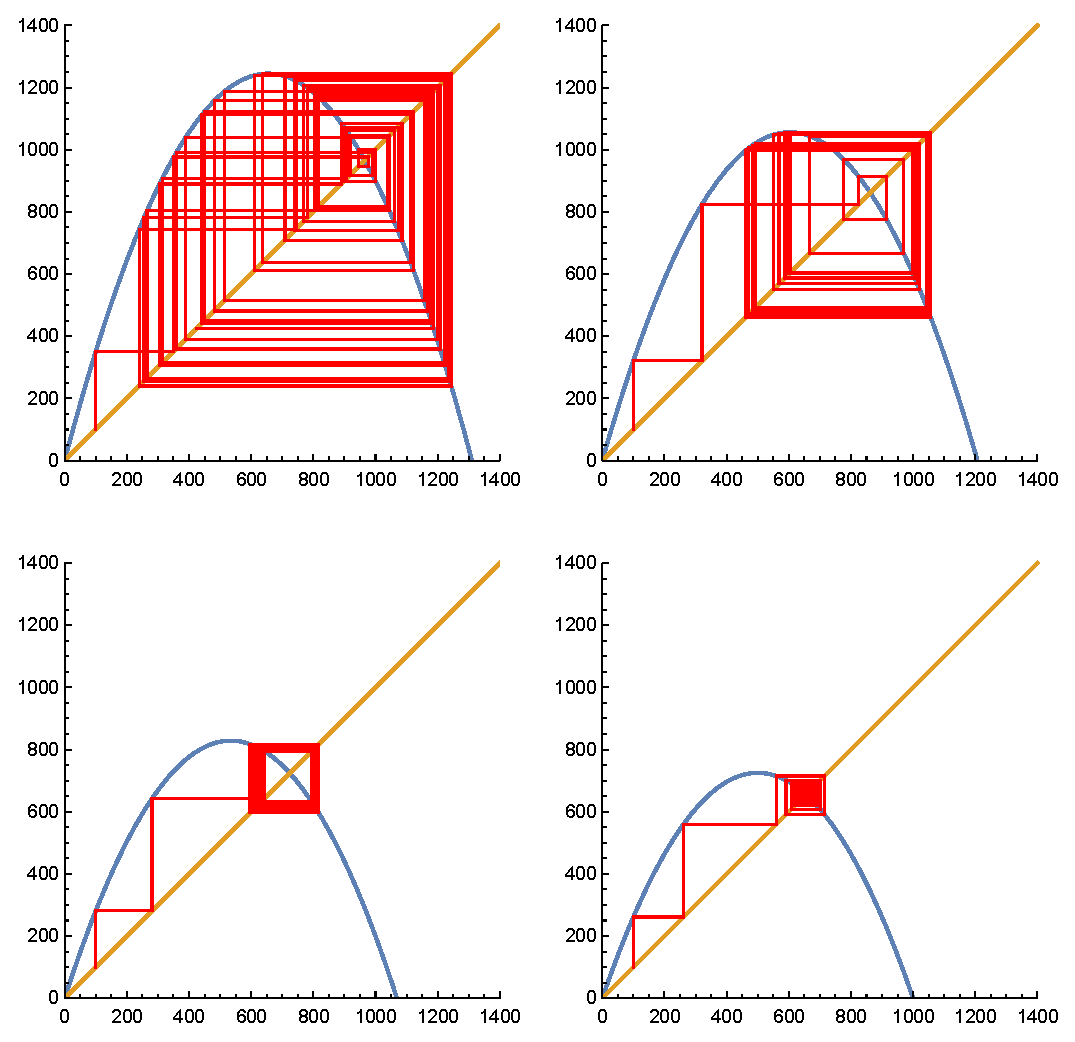
\includegraphics[scale=.7]{harvestdynamics2} 
\caption{Cobweb diagram (see Code box~\ref{code:verhulst}) showing how the stock size (at time $t$ along the horizontal axis and at time $t+1$ along the vertical axis) is adjusted according to an increasing fishing effort. The discrete time model (blue curve) is given by Equation~\ref{eq:discrete population growth} and the four cases illustrate how the increasing fishing effort $E$ dampens the seemingly chaotic behaviour (top left) towards stable equilibriums (limited cycles and equilibrium point in the lower right plot). The yellow lines represent stock biomass equilibriums and the red lines display the dynamics over time with an initial stock size of 100.\\}
\label{fig:cobwebharvest2}
\end{figure}
\hfill \break
Figure~\ref{fig:cobwebharvest2} illustrates the stabilising effect increasing harvest has on the dynamics pictured in Figure~\ref{fig:cobwebharvest}. In Figure~\ref{fig:cobwebharvest2} the intrinsic growth rate is constant (and high) while the fishing effort increases from top left to lower right.

%------------------------------------------------
\section{Equilibrium harvest and surplus production}\index{Surplus production!Equilibrium harvest}\label{harvestsurplus}
We see that the given assumptions of a bi-linear catch equation (Equation~\ref{eq:schaeffer}) and a parabolic growth equation leads a parabolic equilibrium harvest equation in fishing effort (as in the top row of Figure~\ref{fig:surplusharvest}). This is a result of the symmetry of a parabolic equations and the assumed linear short term catch equation. The equilibrium catch may describe a very different curve than the the surplus production growth, both depending on the shape of the growth curve and the short term catch equation. 

In all cases, however, there is a very important distinction to do with regard of the two equations illustrated in Figure~\ref{fig:surplusharvest}, $f(X)$ and $H(E)$. While the first describes a path toward the natural equilibrium $K$, the other is simply a collection of equilibriums. Any position on the curve described by $H(E)$ is fixed and there is by definition impossible to assume any change in the system without leaving the curve (or collection of infinitely many equilibriums).

\begin{figure}[ht]
\centering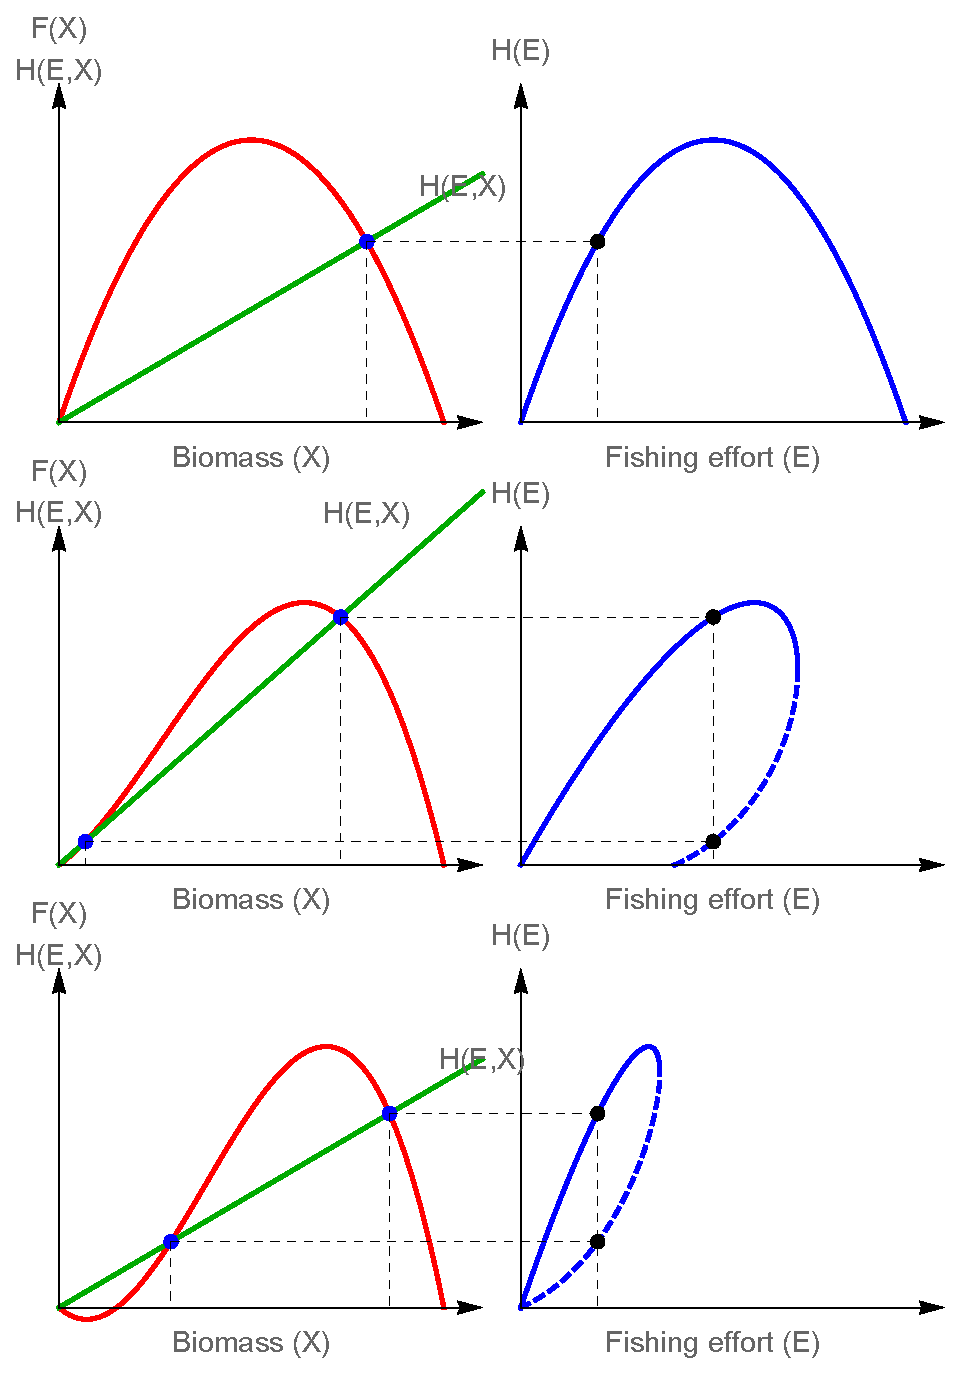
\includegraphics[scale=.5]{surplusharvest}
\caption{Illustration showing the relationship between biological surplus production (red curves to the left) and equilibrium harvest (blue curves to the right) of three different cases of biological growth. The three cases are: logistic growth (top row), depensatory growth (mid row) and critical depensatory growth (bottom row, see Code box~\ref{code:depensation}). The two latter include unstable equilibriums on the blue curves indicated by a dashed curve. In all cases the biological growth and a bilinear harvest equation ($H(E,X)$, the green lines to the left) determine the path of the blue curves for different values of fishing effort ($E$).}
\label{fig:surplusharvest}
\end{figure}
\begin{figure}[!htb]
\begin{remark}
\rule{\linewidth}{.1pt}
\floatbox[{\capbeside\thisfloatsetup{capbesideposition={right,top},capbesidewidth=11.8cm}}]{figure}[\FBwidth]
{\caption*{\footnotesize{Equilibrium harvest related to different surplus\\production models: 

\href{http://demonstrations.wolfram.com/SurplusProductionModelsAndEquilibriumHarvest/}{\\ http://demonstrations.wolfram.com/\\SurplusProductionModelsAndEquilibriumHarvest/}}}}
{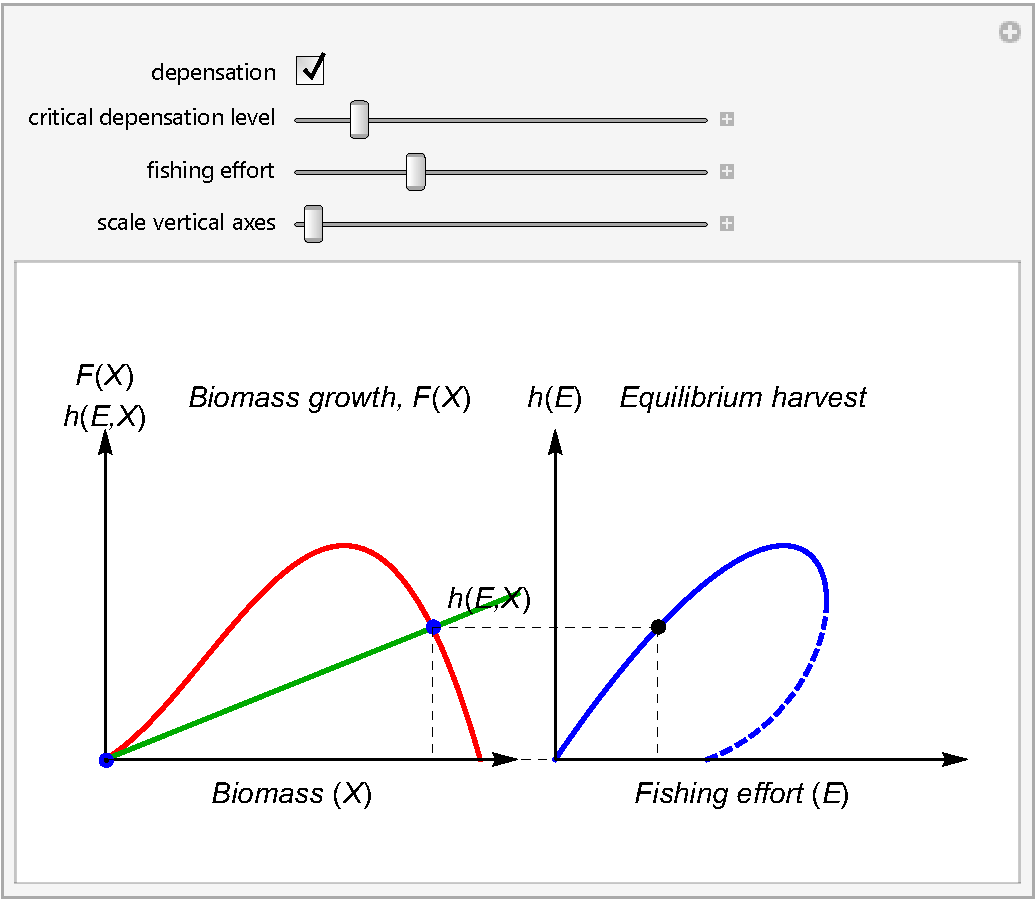
\includegraphics[width=2.8cm]{demo_equilibriumharvest}}\\
\rule[10pt]{\linewidth}{.1pt}\end{remark}\end{figure}

%------------------------------------------------
\section{Sustainable yield in age structured models}\index{Age structured models!Equilibrium harvest}\label{agestructuredF}
In age structured models the catch needs to be distributed on age groups, hence the catch becomes an integral part of the stock dynamics by affecting age composition and strength. The natural mortality ($M$ in equation~\ref{eq:mortality}) is often assumed to be constant for all age groups (while the natural mortality usually is higher in the earliest stages of life this assumption also follows an assumed recruitment age sufficiently high to make it reasonable to assume constant natural mortality) the fishing mortality rate may vary between age groups. Of particular importance is the age of first catch ($t_c$) which has a great impact on the sustainable catch level in a fishery expressed by an age structured model (see code box~\ref{code:bevertonandholt}).

Fishing mortality, as expressed by the fishing mortality rate $F$, is an expression of the production of fishing effort which is described in chapter~\ref{chapter 2}. From equation~\ref{eq:cobbdouglas3} we see how catch may be expressed as a function of fishing effort ($E$) and stock biomass ($X$). Substituting fishing effort by the biological fishing mortality rate simplify the expression to
\begin{equation} 
\label{eq:production2}
H(F,X) = F \cdot X
\end{equation}
When $H(F,X) = H(E,X)$ (from equation~\ref{eq:cobbdouglas3}) we can express the fishing mortality as a function of produced fishing effort the current stock biomass:
\begin{equation} 
\label{eq:FErelation}
F(E,X) = q \cdot E^{\alpha} \cdot X^{\beta-1}
\end{equation}
When $\alpha = \beta = 1$ this simplifies to $F = q \cdot E$.

The corresponding fishing effort (the inverse of equation~\ref{eq:FErelation}, expressed as a function of fishing mortality rate and stock size) is: 
\begin{equation} 
\label{eq:EFrelation}
E(F,X) =\bigg(\frac{F \cdot X^{1-\beta}}{q}\bigg)^{\frac{1}{\alpha}}
\end{equation}
In the code box below a constant fishing mortality rate ($F$) is assumed after the age of first catch ($t_c$) in the stock. A varying selective pattern is however more realistic in a fishery. The selective pattern depends on a number of factors, first of all the properties of the gear (see figure~\ref{fig:selection}) and spatial and temporal distributions of year classes and fishing activities.

\begin{theorem}[Age structured model (Beverton and Holt)]
\hfill \break
%\mmaCellGraphics[form=TraditionalForm]{Output}{pg1.pdf}
Continuing from code box~\ref{code:cohortbiomass}

TotalCatch is the yield function in the PopulationGrowth package, including two variables defining an equilibrium fishery: The fishing mortality rate $F$ and the age of the cohort first recruited to the fishable stock, $t_c$. Below we assume sharp selection at age $t_c$ at which a constant fishing mortality rate is imposed. The total catch has no other analytic expression than the simple product of $F$ (the fishing mortality rate) and $X$ (the stock biomass) without specifying a minimum of parameter values:
\begin{mmaCell}[index=16]{Input}
  TotalCatch[] // Notation
\end{mmaCell}

\includegraphics[scale=.85]{bh1}

A complex analytical expression (including $\beta$ and $\gamma$ functions) is found for \texttt{InitialAge -> 0}. A more readable expression is found by setting the \texttt{WeightLengthRelation} equal 3 and including an infinite number of cohorts:
\begin{mmaCell}{Input}
  TotalCatch[
    OldestAge            -> Infinity, 
    WeightLengthRelation -> 3
  ] // SimplifyNotation
\end{mmaCell}

\includegraphics[scale=.85]{bh2}

A further simplification for the case when the natural mortality rate equals the natural growth rate ($M = k$):
\begin{mmaCell}{Input}
  TotalCatch[
    InitialAge           -> 0, 
    WeightLengthRelation -> 3,
    OldestAge            -> Infinity,
    MortalityRate        -> GrowthRate, 
    RecruitmentAge       -> 0
  ] // SimplifyNotation
\end{mmaCell}

\includegraphics[scale=.85]{bh3}

And finally:
\begin{mmaCell}{Input}
  TotalCatch[
    CatchAge             -> 0, 
    OldestAge            -> Infinity,
    InitialAge           -> 0, 
    RecruitmentAge       -> 0,
    MaxWeight            -> 1, 
    MortalityRate        -> GrowthRate,
    WeightLengthRelation -> 3
  ] // SimplifyNotation
\end{mmaCell}

\includegraphics[scale=.85]{bh4}

Let us use the parameter values from input number 9 and plot the surface of the yield function in the $F-t_c-$plane, employing the Plot3D function in \textit{Mathematica}:
\index{\texttt{Plot3D}}\index{\texttt{Sequence}}
\begin{mmaCell}{Input}
  Plot3D[
    TotalCatch[Sequence @@ values], 
    \{F, 0, 1\}, \{tc, 0, 20\},
    PlotPoints    -> 35, 
    PlotRange     -> All, 
    MeshFunctions -> \{#3 &\}, 
    Mesh          -> 10, 
    PlotLabel     -> "Sustainable Yield per recruit (kg)", 
    AxesLabel     -> \{
      "Fishing mortality rate (F)", "Selection age \mmaSub{t}{c}", ""\}
    ]
\end{mmaCell}
\begin{mmaCell}[moregraphics={moreig={scale=.9}}]{Output}
  \mmaGraphics{pg5}
\end{mmaCell}
This is the function shown in the plot above:
\begin{mmaCell}{Input}
  TotalCatch[Sequence @@ values]
\end{mmaCell}
\begin{mmaCell}{Output}
  -10 \mmaSup{e}{-0.2 tc} F \bigg(-\mmaFrac{1}{0.2 + F} + \mmaFrac{3 \mmaSup{e}{-0.2 tc}}{0.4 + F} - \mmaFrac{3 \mmaSup{e}{-0.4 tc}}{0.6 + F} + \mmaFrac{\mmaSup{e}{-0.6 tc}}{0.8 + F}\bigg)
\end{mmaCell}
Maximum Sustainable Yield for any given value of $t_c$ defines a curve in the $F-t_c$ area.
\index{\texttt{Range}}\index{\texttt{FindMaximum}}\index{\texttt{Sequence}}
\begin{mmaCell}{Input}
  MSYCurve = \{F /. FindMaximum[
    TotalCatch[
      FishingMortalityRate -> F, 
      CatchAge             -> #, 
      Sequence @@ values,
      BiomassIncluded      -> Fishable
    ],
    \{F, .01\}, 
    PrecisionGoal -> 5, 
    AccuracyGoal  -> 5, 
    Method        -> "PrincipalAxis"
  ][[2]], #\} & /@ Range[0, 6, .2];
\end{mmaCell}
In the same way the Eumetric curve is defined by maximising harvest at any given fishing mortality rate value.
\index{\texttt{Range}}\index{\texttt{FindMaximum}}\index{\texttt{Join}}
\begin{mmaCell}{Input}
  EumetricCurve = \{#[[1]], tc /. #[[2]]\} & /@ (
  \{#, FindMaximum[
      TotalCatch[
        FishingMortalityRate -> #, 
        Sequence @@ values, 
        BiomassIncluded      -> Fishable
      ],
      \{tc, 3\}, 
      PrecisionGoal -> 5, 
      AccuracyGoal  -> 5
    ][[2]]\} & /@ Join[
      (.001 + .005*(# - 1)) & /@ Range[81],
      (.4 + .2*#) & /@ Range[20]
    ]);
\end{mmaCell}
By using the \texttt{ContourPlot} function it is straight forward to produce isopleth diagrams which are heavily used by Beverton and Holt\cite{Beverton1957} and in which we can draw the MSY curve and the Eumetric curve:
\index{\texttt{ListLinePlot}}\index{\texttt{Show}}\index{\texttt{ContourPlot}}
\begin{mmaCell}{Input}
  Show[\{
    ContourPlot[
      TotalCatch[Sequence @@ values],
        \{F, 0, 1\}, \{tc, 0, 10\},
        PlotPoints     -> 50, 
        ContourShading -> False, 
        ContourStyle   -> Thick,
        Contours       -> 10
      ],
      ListLinePlot[\{EumetricCurve, MSYCurve\}, 
        PlotStyle   -> \{Directive[Red, Thick], 
          Directive[Darker@Green, Thick]\},  
        PlotLegends -> \{"Eumetric curve", "MSY curve"\}
      ]
    \},
    FrameLabel       -> \{"F", "\mmaSub{t}{c}"\}, 
    PlotRangePadding -> None
  ]
\end{mmaCell}
\begin{mmaCell}[moregraphics={moreig={scale=.8}}]{Output}
  \mmaGraphics{bh5}
\end{mmaCell}
\label{code:bevertonandholt}
\end{theorem}
\hfill \break
Since the age structured model presented in Code Box~\ref{code:bevertonandholt} includes two control variables, the fishing mortality rate $F$ and $t_c$, the age of recruitment to the exploited fraction of the stock, the equilibrium harvest of output 17 in  Code Box~\ref{code:bevertonandholt} could be maximised at given $t_c$ values, at given values of $F$, or the other way around. The dual problems are to minimise the values of $F$ or $t_c$ for given equilibrium harvest.

The path obtained by minimising the fishing mortality rate $F$ for given equilibrium harvest is by Beverton and Holt referred to as the \textit{eumetric} curve (see code box~\ref{code:bevertonandholt})\cite{Beverton1956}. We will discuss the economic interpretation of the eumentric curve in another chapter. The other curve displayed in output 24 of Code Box~\ref{code:bevertonandholt} is the $MSY$ curve. The global maximum of sustainable yields in the age-structured model is obtained at an infinitely high fishing mortality rate, targeting the fish at the age when the biomass of one cohort is maximised (see input and output 10 in code box~\ref{code:cohortbiomass}). Maximising the yield for all the other possible $t_c$ values describes a $MSY$ curve through the $F-t_c$ plane as shown in output 24 of code box~\ref{code:bevertonandholt}.

\index{Fishing gears!Gill net}The Maximum Sustainable Yield ($MSY$), which in Equation~\ref{eq:msy} is one point, in the age-structured model describes a path in the $F-t_c$ plane. 

\begin{figure}[!htb]
\begin{remark}
\rule{\linewidth}{.1pt}
\floatbox[{\capbeside\thisfloatsetup{capbesideposition={right,top},capbesidewidth=11.8cm}}]{figure}[\FBwidth]
{\caption*{\footnotesize{Investigate the Beverton and Holt model under different\\parametrisations at

\href{http://demonstrations.wolfram.com/BevertonAndHoltsYieldPerRecruitModel/}{\\ http://demonstrations.wolfram.com/\\BevertonAndHoltsYieldPerRecruitModel/}}}}
{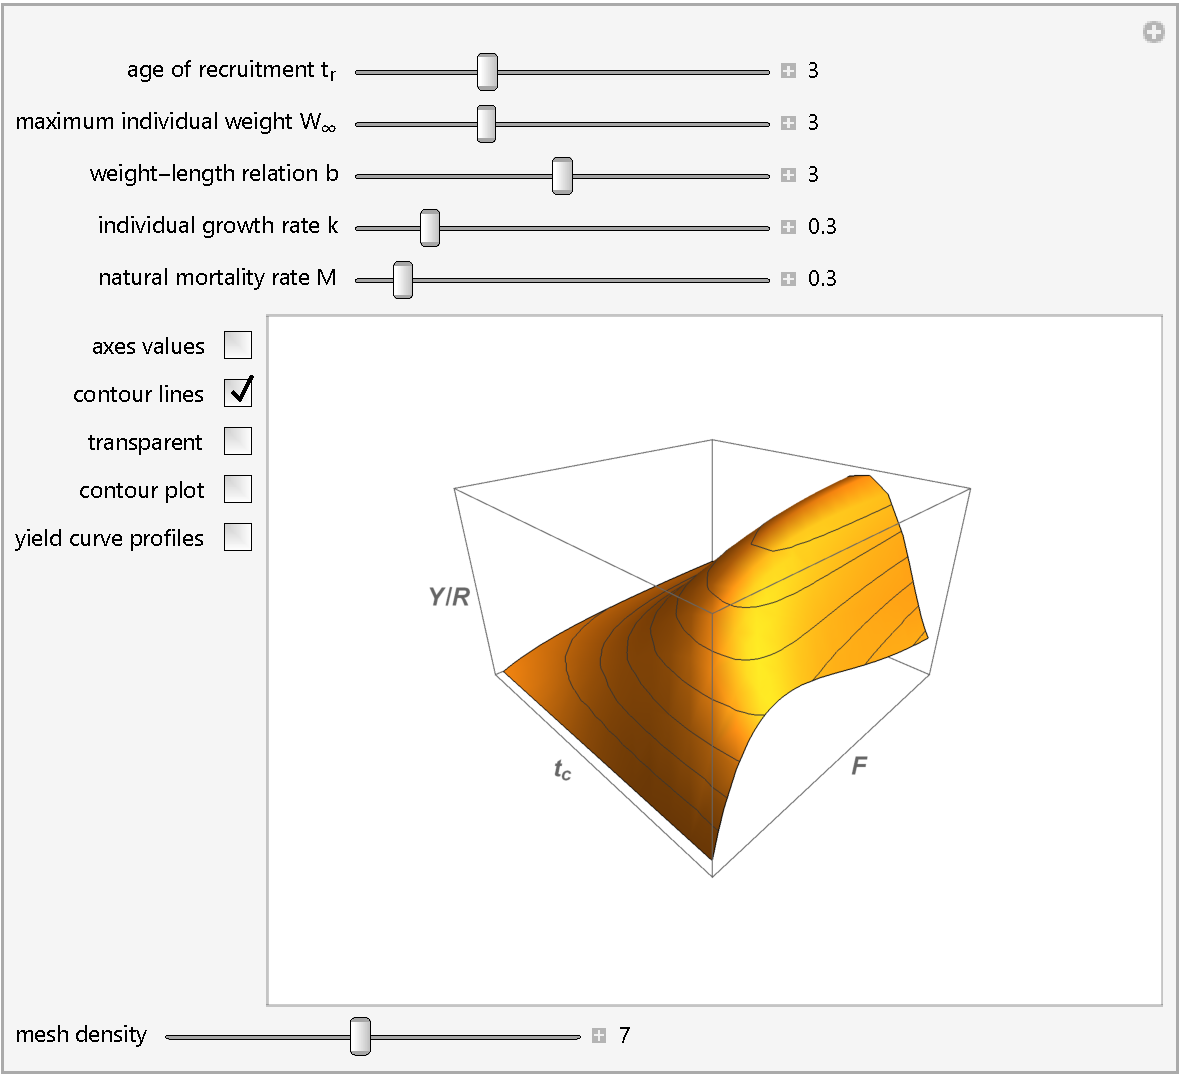
\includegraphics[width=2.8cm]{demo_BevertonHolt}}\\
\rule[10pt]{\linewidth}{.1pt}\end{remark}\end{figure}

\newpage

%------------------------------------------------
\section{Cellular automata modelling}\index{Cellular automata modelling}

\begin{figure}[!htb]
\begin{remark}
\rule{\linewidth}{.1pt}
\floatbox[{\capbeside\thisfloatsetup{capbesideposition={right,top},capbesidewidth=11.8cm}}]{figure}[\FBwidth]
{\caption*{\footnotesize{Explore a 1D cellular automata model in which Marine\\Protected Area (MPA) is implemented as a regulatory measure at 

\href{http://demonstrations.wolfram.com/CellularAutomataModelOfAnMPAFishery/}{\\ http://demonstrations.wolfram.com/\\CellularAutomataModelOfAnMPAFishery/}}}}
{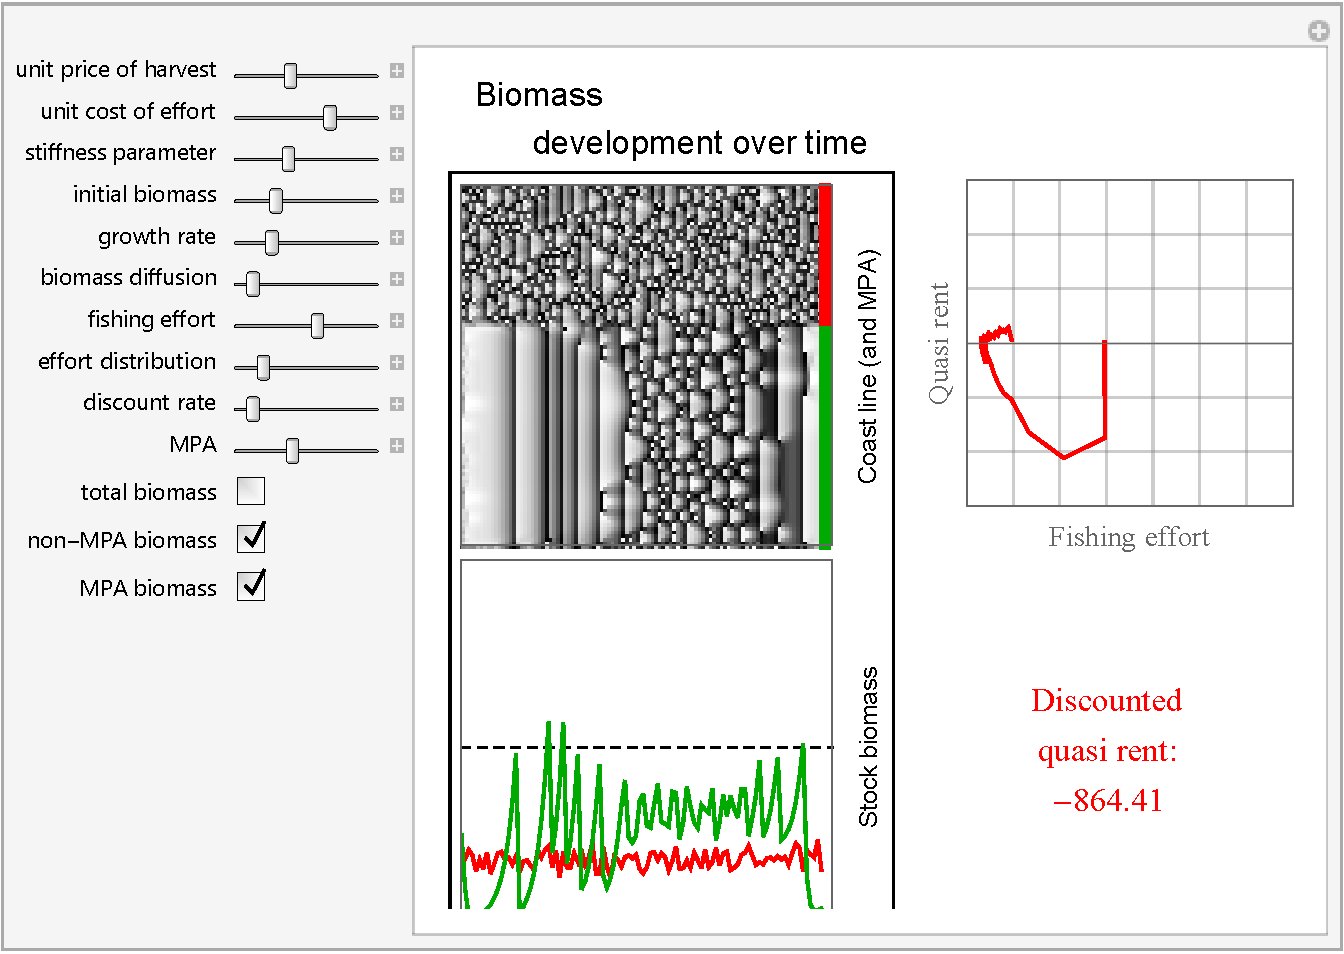
\includegraphics[width=2.8cm]{demo_CA_MPA}}\\
\rule[10pt]{\linewidth}{.1pt}\end{remark}\end{figure}

%------------------------------------------------
\section{Stage structured fishery models}\index{Stage structured fishery models}

\begin{figure}[!htb]
\begin{remark}
\rule{\linewidth}{.1pt}
\floatbox[{\capbeside\thisfloatsetup{capbesideposition={right,top},capbesidewidth=11.8cm}}]{figure}[\FBwidth]
{\caption*{\footnotesize{Explore the discrete Ricker population model with delayed\\recruitment at 

\href{http://demonstrations.wolfram.com/BioeconomicsOfADiscreteRickerModelWithDelayedRecruitment/}{\\ http://demonstrations.wolfram.com/\\BioeconomicsOfADiscreteRickerModelWithDelayedRecruitment/}}}}
{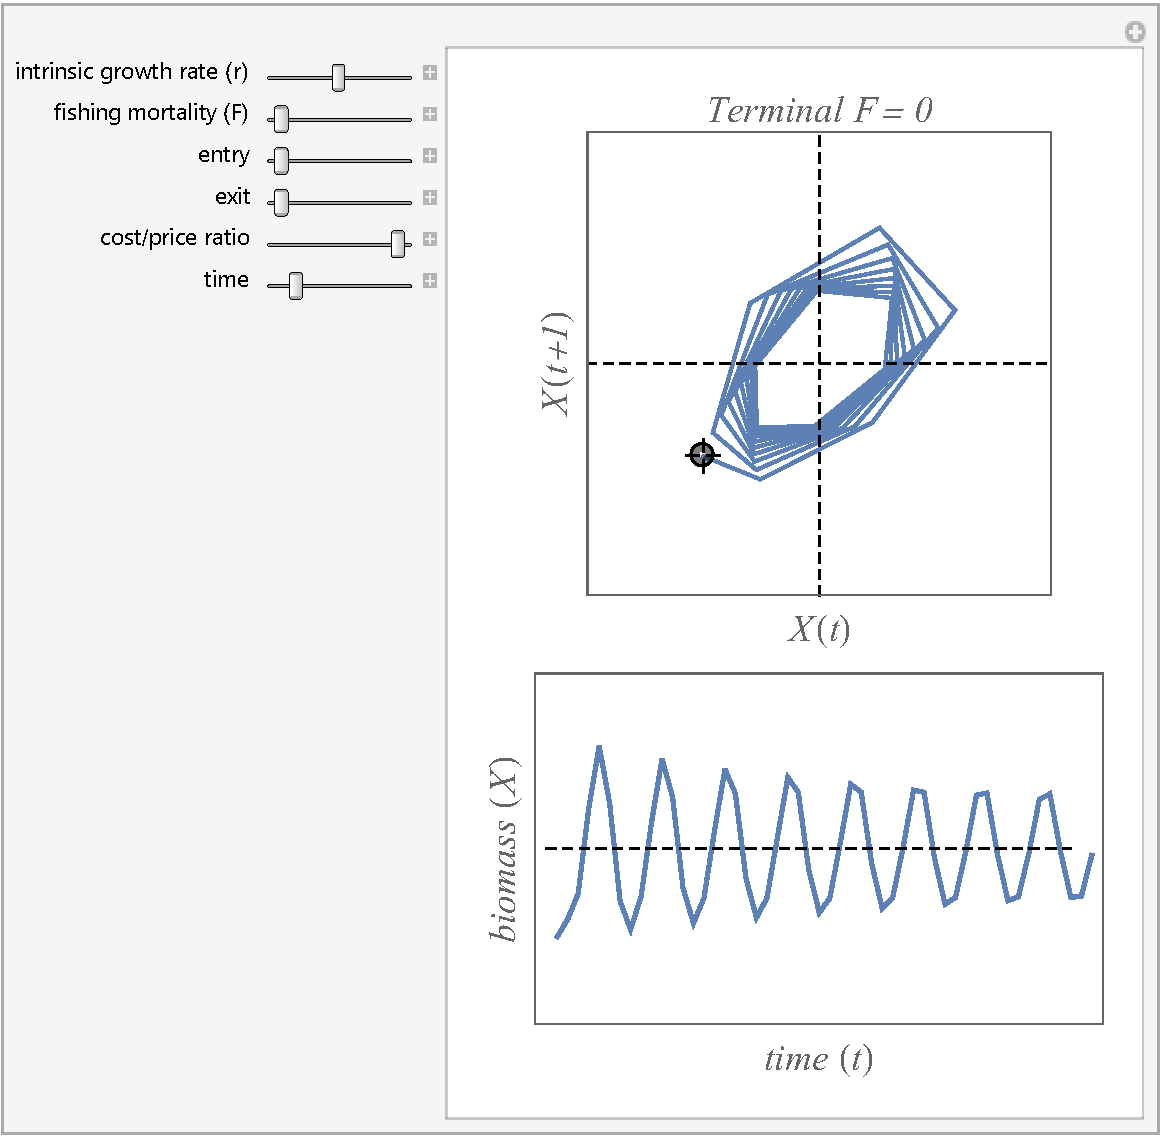
\includegraphics[width=2.8cm]{demo_Ricker}}\\ 
\rule[10pt]{\linewidth}{.1pt}\end{remark}\end{figure}

%------------------------------------------------
\section*{Exercises}\index{Exercises!Chapter 5}
\addcontentsline{toc}{section}{Exercises}

\begin{exercise}
At which stock size is $MSY$ obtained in the case of Equation~\ref{eq:eqharvest}?
\end{exercise}




\part{Fisheries economics}
%========================================================================================
%	P A R T   2
%========================================================================================

\chapterimage{h6.jpg} % Chapter heading image
%------------------------------------------------
\chapter{The economics of catch production} \label{chapter 6}
%----------------------------------------------------------------------------------------
%	CHAPTER 6
%----------------------------------------------------------------------------------------
\index{Production functions!Cost of production}
Fishing is an economic activity. So far we have focused the fishing technology and factors needed to produce harvest. The production functions we have discussed all assumes technological efficiency, that no input factors are wastes. The production functions therefore gives the lowest quantities of production factor by which it is technological possible to produce a given output quantity. Now we will try to identify which of these combinations of minimum factor levels that also are economically efficient.

\section{The economics of effort production}\label{section: open access}

While technological efficiency is assumed in the production functions we have described, we will now introduce the concept of economic efficiency. There are two approaches to economic efficiency in production, minimising cost of a given production or maximising production within a given budget. In the box below we provide the \textit{Mathematica} code following the latter principle.

In order to study economic efficiency in production we need to have an expression for the cost of production. We assume the production function in equation~\ref{eq:cobbdouglas2} and assume constant market prices for the two input factors, labour ($l$) and capital ($k$). Let the price (wage) of labour be $w$ and the price (interest rate) of capital be $i$. The total cost of a consuming labour and capital in the production process then is
\begin{equation} 
\label{eq:costofproduction}
C(L,K) = w \cdot L + i \cdot K
\end{equation}

\begin{theorem}[Economic efficiency in production]
\hfill \break
The Cobb-Douglas function with constant elasticity of scale equal $\alpha + \beta$:
\begin{mmaCell}[index=1]{Input}
  cd[l_, k_] := A * l^\(\pmb{\alpha}\) * k^\(\pmb{\beta}\)
\end{mmaCell}
The cost of production,$w$ being the cost of labour and $i$ the cost of capital:
\begin{mmaCell}[index=2]{Code}
  c[l_, k_] := w*l + i*k
\end{mmaCell}
The problem is to maximise the production within a given budget restriction $R$. We formulate the Lagrange equation for the problem of constrained maximisation:
\begin{mmaCell}[index=3]{Input}
  lagrange[l_, k_] := cd[l, k] - \(\pmb{\lambda}\) (R - c[l, k])
\end{mmaCell}
\index{\texttt{D} (Derivative)}\index{\texttt{Solve}}\index{\texttt{Sequence}}
\begin{mmaCell}{Input}
  Sequence@@Solve[
    ((\(\pmb{\lambda}\) /. Solve[D[lagrange[l, k], l] == 0, \(\pmb{\lambda}\)][[1]]) ==
      (\(\pmb{\lambda}\) /. Solve[D[lagrange[l, k], k] == 0, \(\pmb{\lambda}\)][[1]])) /. \{
      l -> k * x\}, x
    ][[1]] /. \{x -> l/k\}
\end{mmaCell}
\begin{mmaCell}{Output}
  \mmaFrac{l}{k} \(\to\) -\mmaFrac{i \(\pmb{\alpha}\)}{w \(\pmb{\beta}\)}
\end{mmaCell}
\label{code:cdcost}
\end{theorem}

From the calculation in Code box~\ref{code:cdcost} we see that technologically and economic efficient Cobb-Douglas production is obtained when the following condition is met
\begin{equation} 
\label{eq:cdefficiency}
\frac{L}{K} = -\frac{i \cdot \alpha}{w \cdot \beta}
\end{equation}

We see that the ratio between the two input factors changes when one of the prices changes. When the wages ($w$) increases, the use of labour ($L$) is reduced and substituted by capital ($K$) if the previous production level should be maintained. We also see that the output elasticities of labour and capital affect how labour is substituted by capital.

From expression~\ref{eq:cdefficiency} we can see that the cost efficient mix of input factors is fixed for given prices ($i$ and $w$) and given output elasticities($\alpha$ and $\beta$). The expansion path described by the optimal mix when regarding different production levels therefore is linear, as shown in Code box~\ref{code:expansionpaths} below.

Expression~\ref{eq:cdefficiency} can be converted to an equation where the efficient amount of capital ($K$) is explained by the use of labour ($L$)
\begin{equation} 
\label{eq:cdefficiency2}
K(L) = \frac{w \cdot \beta}{i \cdot \alpha} \cdot L
\end{equation}

\begin{theorem}[Economic efficient expansion paths in production]
\hfill \break
We start as previously by defining the Cobb-Douglas function:
\begin{mmaCell}[index=1]{Input}
  cd[l_, k_] := A * l^\(\pmb{\alpha}\) * k^\(\pmb{\beta}\)
\end{mmaCell}
The cost equation (equation~\ref{eq:costofproduction}):
\begin{mmaCell}[index=2]{Code}
  c[l_, k_] := w*l + i*k
\end{mmaCell}
Cost efficient input of capital as a function of labour input is found from expression~\ref{eq:cdefficiency2}:
\begin{mmaCell}{Input}
  k[l_] := l * w * \(\pmb{\beta}\) / (i * \(\pmb{\alpha}\))
\end{mmaCell}
Now we plot the directions of the expansion paths for different values of $\alpha$ and $\beta$. The elasticity of scale ($\epsilon$ = $\alpha$ + $\beta$)in first three plots equal one, while the last plot shows a case where $\epsilon$ = $\alpha$ + $\beta$ = 1 + 1 = 2:
\index{\texttt{Show}}\index{\texttt{Plot}}\index{\texttt{GraphicsGrid}}\index{\texttt{ContourPlot}}\index{\texttt{Partition}}\index{\texttt{ToString}}
\begin{mmaCell}{Input}
  GraphicsGrid[
    Partition[
      Show[\{
        ContourPlot[cd[l, k] /. \{
            A -> 1, \(\pmb{\alpha}\) -> #,  \(\pmb{\beta}\) -> If[# < 1, 1 - #, 1]\}, 
          \{l, 0, 1\}, \{k, 0, 1\}, 
          ContourShading -> None, 
          Contours -> \{.02, .1, .2, .4, .6, .8\}
        ],
        Plot[k[l] /. \{
            \(\pmb{\alpha}\) -> #, \(\pmb{\beta}\) -> If[# < 1,1 - #, 1], w -> 1, i -> 1\}, 
          \{l, 0, 1\}, 
          PlotStyle -> Red
        ]\},
        PlotLabel -> "\(\pmb{\alpha}\) = " <> ToString[#] <> ",
          \(\pmb{\beta}\) = " <>  ToString[If[# < 1,1 - #, 1]],
        FrameLabel -> \{"Labour (L)", "Capital (K)"\},
        FrameTicks -> None
      ] & /@ \{.3, .5, .7, 1\}, 2
    ], 
    Spacings -> \{0, 20\}
  ]
\end{mmaCell}
\begin{mmaCell}[moregraphics={moreig={scale=.8}}]{Output}
  \mmaGraphics{exppath}
\end{mmaCell}
Note that the red expansion path in the case of $\alpha$ = $\beta$ = 0.5 is similar to the case when $\alpha$ = $\beta$ = 1. From expression~\ref{eq:cdefficiency} it is easy to see that this indeed must be true. The production level of the latter case increases, however, at the rate 2:1 compared with the first case.
\label{code:expansionpaths}
\end{theorem}

As described in Section~\ref{cesf} the elasticity of substitution of the Cobb-Douglas function is one. In a normal production process also the elasticity of scale is expected to equal one, as in equation~\ref{eq:cobbdouglas}. The plots in Code box~\ref{code:expansionpaths} also display the case of $\epsilon > 1$, representing cases where there are economics of scale.

\begin{theorem}[Unit cost of production]
\hfill \break
Let us continue from Code box~\ref{code:expansionpaths}. Let us further assume that $\beta = 1 - \alpha$, as in equation~\ref{eq:cobbdouglas}. The unit cost of production is equation~\ref{eq:costofproduction} divided by equation~\ref{eq:cobbdouglas} when including equation~\ref{eq:cdefficiency2}. When specifying basic assumptions we find
\index{\texttt{Simplify}}\index{\texttt{Element}}
\begin{mmaCell}{Input}
  Simplify[
    c[l, k[l]] / cd[l, k[l]] /. \{\(\pmb{\beta}\) -> 1 - \(\pmb{\alpha}\)\}, 
    Assumptions -> \{
      Element[\{l, w, i, A, \(\pmb{\alpha}\)\}, Reals], 
        w > 0, i > 0, l > 0, A > 0, 0 < \(\pmb{\alpha}\) < 1\}
    ]
\end{mmaCell}
\begin{mmaCell}{Output}
  -\mmaFrac{i \mmaSup{(i \(\pmb{\alpha}\))}{-\(\pmb{\alpha}\)} \mmaSup{(w - w \(\pmb{\alpha}\))}{\(\pmb{\alpha}\)}}{A (- 1 + \(\pmb{\alpha}\))}
\end{mmaCell}
From this result we can conclude that for a Cobb-Douglas production process with elasticity of scale equal one, the unit cost of output is constant in an economically efficient production.

As seen below this is not necessarily the case when the elasticity of scale is different from one:
\index{\texttt{Simplify}}\index{\texttt{Element}}
\begin{mmaCell}{Input}
  Simplify[
    c[l, k[l]] / cd[l, k[l]], 
    Assumptions -> \{
      Element[\{l, w, i, A, \(\pmb{\alpha}\), \(\pmb{\beta}\)\}, Reals],
        w > 0, i > 0, l > 0, A > 0, 0 < \(\pmb{\alpha}\) < 1, 0 < \(\pmb{\beta}\) < 1\}
    ]
\end{mmaCell}
\begin{mmaCell}{Output}
  \mmaFrac{\mmaSup{l}{1-\(\pmb{\alpha}\)} w \mmaSup{(i \(\pmb{\alpha}\))}{\(\pmb{\beta}\)} \mmaSup{(l w \(\pmb{\beta}\))}{-\(\pmb{\beta}\)} (\(\pmb{\alpha}\) + \(\pmb{\beta}\))}{A \(\pmb{\alpha}\)}
\end{mmaCell}
In the special case of $\alpha = \beta = 1/2$ the unit price of production is found to be
\index{\texttt{Simplify}}\index{\texttt{Element}}
\begin{mmaCell}{Input}
  Simplify[
    c[l, k[l]] / cd[l, k[l]] /. \{\(\pmb{\alpha}\) -> 1/2, \(\pmb{\beta}\) -> 1/2\}, 
    Assumptions -> \{
      Element[\{l, w, i, A\}, Reals], w > 0, i > 0, l > 0, A > 0\}
  ]
\end{mmaCell}
\begin{mmaCell}{Output}
  \mmaFrac{2 \mmaSqrt{i w}}{A}
\end{mmaCell}
\label{code:unitcost}
\end{theorem}

%------------------------------------------------
\section{Total cost and revenue}\index{Total cost and revenue}\label{TC and TR}

As shown in code box~\ref{code:unitcost} constant unit cost of effort production may be a reasonable assumption. Let us assume a constant unit cost of effort equal $a$. Assume further that the unit cost includes all costs, also the opportunity costs of labour and capital. Hence, the cost embeds a normal profit, e.g. a \textit{normal profit} \index{Normal profit} is obtained when the income covers the cost. The total cost ($TC$) of producing fishing effort $E$ then is
\begin{equation} 
\label{eq:TC}
TC(E) = a \cdot E
\end{equation}
Furthermore, let us assume a constant unit price of harvest, $p$, and assume an equilibrium catch equation as for example Equation~\ref{eq:eqharvest}. The total revenue in the fishery ($TC$) then is
\begin{equation} 
\label{eq:TR}
TR(E) = p \cdot H(E)
\end{equation}
Since a normal profit is embedded in the unit cost of effort ($a$), total economic rent in the fishery ($R$), often referred to as abnormal or supernormal rent, is given by the difference between TR and TC:
\begin{equation} 
\label{eq:R}
R(E) = TR(E) - TC(E)
\end{equation}

\begin{figure}[ht]
\centering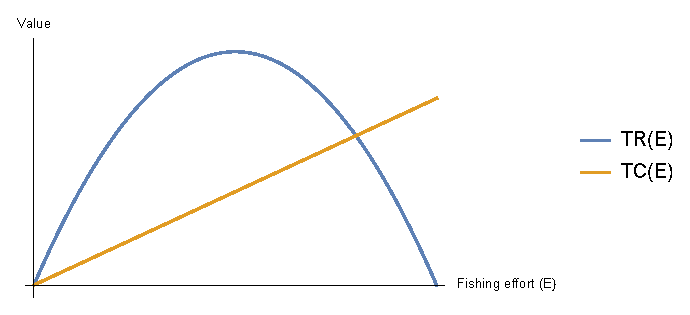
\includegraphics[scale=1.]{TRandTC}
\caption{The figure shows a possible relationship between TC (Equation~\ref{eq:TC}) and TR (Equation~\ref{eq:TR}).}
\label{fig:TRandTC}
\end{figure}

%------------------------------------------------
\section{Economic rent in fisheries}\index{Economic rent in fisheries}\label{rent}

According to \textit{The New Palgrave Dictionary of Economics}, "\textit{Rent} is the payment for use of a resource, whether it be land, labour, equipment, ideas, or even money"\cite{Alchian1987}. The rent for labour is called \textit{wages} and the payment for money is called \textit{interest}. Payment for a resource which availability is insensitive to the size of the payment is called \textit{economic rent}, if the insensitivity is permanent or \textit{quasi-rent} if the insensitivity is temporary.

The British economist Alfred Marshall (1842 - 1924) did several attempts of clarifying different terms used to characterise different types of rent\cite{Marshall2009PrinciplesEconomics} and was the one to introduce the term \textit{quasi-rent}. For the early classical economists \textit{rent} was synonymous to \textit{land rent}. It soon became evident that this definitions was too narrow and a number of new terms were introduced; such as \textit{differential rent} and \textit{scarcity rent}. Even after Marshall's contributions there are still a lot of confusion related to the use of terms referring to different types of rent. While some economists still stick to the original definitions other employ more modern definitions of the terms.

In the context of this book we will label all payment beyond what may be considered as a \textit{normal profit} as \textit{economic rent}. Economic rent may have different origins and these types of rents may be referred to by specific terms, all of them being within the category of economic rent. Hence, economic rent in a lumped based term including all kinds of abnormal profits, such as \textit{resource rent}, \textit{differential rent}, \textit{quasi rent} and \textit{monopoly rent}. This list illustrates some of the confusion related to the labelling of rent. Resource rent may for example be collected as monopoly rent, while differential rent first of all occurs in the short run as do quasi rent.

\textit{The Ricardian land rent}, named after the British economist David Ricardo (1772 – 1823), is in modern economics referred to by the more general term \textit{resource rent}. \textit{Resource rent} comprises abnormal profits that originate from all kind of natural resources, including fish stock resources.

%------------------------------------------------
\section{The model predicts a homogeneous fleet}\index{Homogeneous fleet}
We assume each decision maker (vessel owner) to follow economic rational behaviour, maximising their individual profit. Assume further that each vessel have a cost pattern with the standard properties we knows from micro economic production theory. The marginal cost of producing fishing effort (the red curves in Figure~\ref{fig:fleetrent}) are declining at low production levels, and reaching a minimum level after which the marginal cost increases by increased production. In this context we regard a normal profit as an opportunity cost included in the cost equation.
\begin{figure}[ht]
\centering
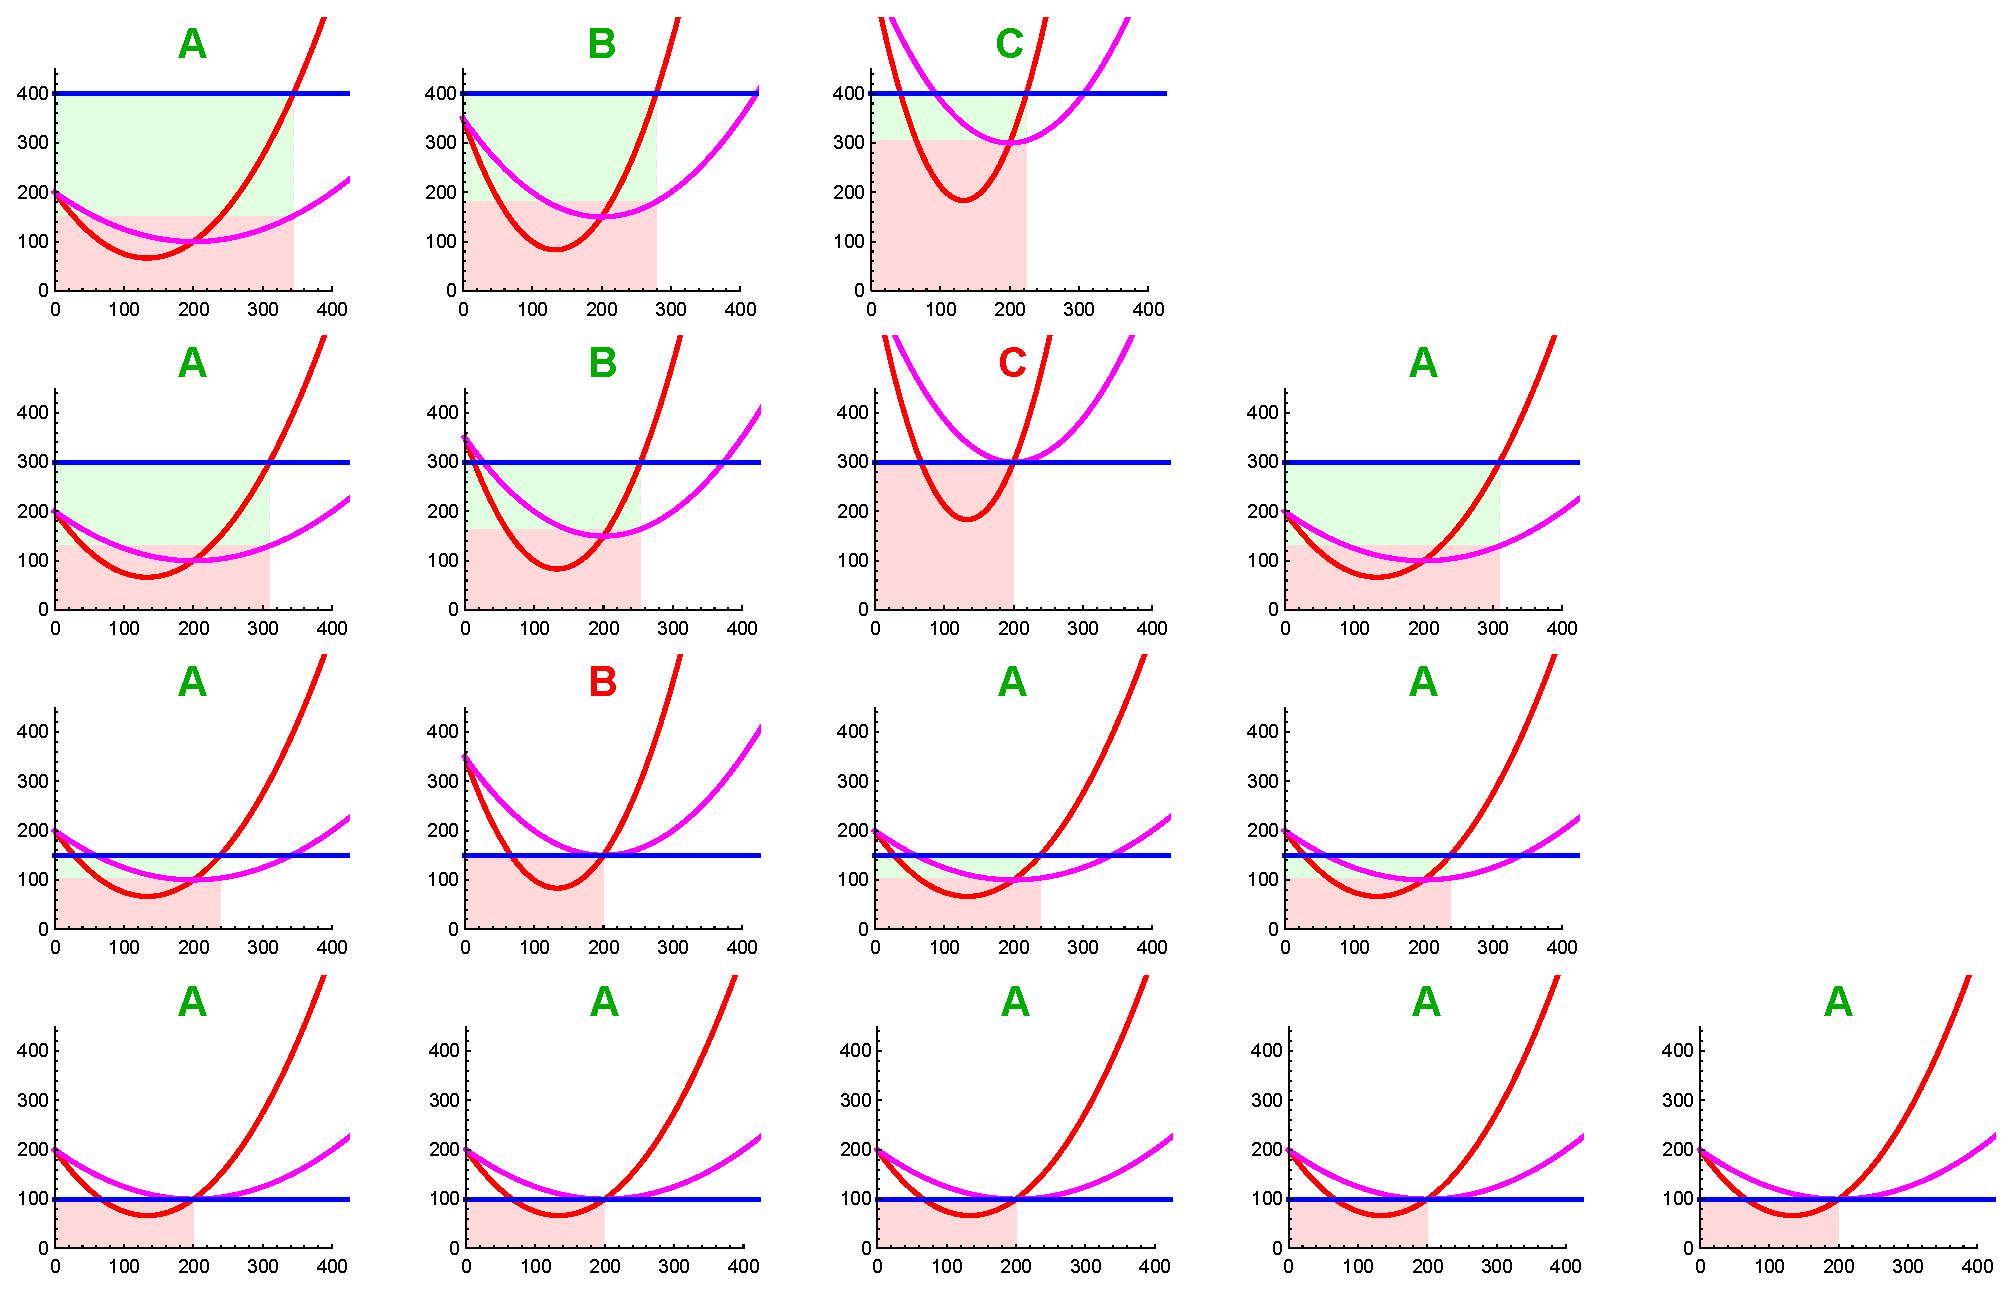
\includegraphics[scale=.44]{fleetrent}
\caption{This figure indicates a possible development in an open access fishery from a diverse fleet (vessels A, B and C in the top line) towards a homogeneous fleet in the bottom line, where all vessels are identical (vessel type A is the most cost efficient). The blue lines are marginal revenues, the red curves are marginal costs and the magenta curves are average costs. The light red areas indicate total cost of production (including a normal profit), while the light green areas are economic rent. As the production of fishing effort increases the marginal revenue declines. The four lines represent a development step by step, where the less cost efficient vessels (type B and C) leave the fishery when they are not able to earn a normal profit.}
\label{fig:fleetrent}
\end{figure}

We assume further that all vessel owners are price takers and that the fishing effort produced by one unit is not sufficient to affect the stock size. In line with equations~\ref{eq:schaeffer} and~\ref{eq:TR} revenue of vessel ($i$) during a given time period therefore is expressed by a constant stock biomass ($X$) and the only variable is the fishing effort produced by the vessel ($u_i$):
\begin{equation} 
\label{eq:unitrevenue}
tr_i = p \cdot q_i \cdot X \cdot u_i
\end{equation} 
where $q_i$ is the vessel specific catchability coefficient and $p$ the constant unit price of harvest. We use the symbol $u$ here to identify the fishing effort produced by one unit (vessel or fisher), not $e$, to avoid confusion with the mathematical constant $e$ (Euler's constant). Total fishing effort is the sum of all unit efforts. For $n$ units we have
\begin{equation} 
\label{eq:sumofunits}
E = \sum_{i=1}^n u_i
\end{equation}
Now we introduce a more general cost equation than the cost equation assumed in equation~\ref{eq:allunitseq}, $tc_i$, including the opportunity costs of labour and capital. The profit maximising vessel will select the fishing effort where the marginal revenue equals the marginal cost:
\begin{equation} 
\label{eq:unitmax}
tc_i'(u_i) = tr_i'(u_i) = p \cdot q_i \cdot X
\end{equation} 
where $X$ is the equilibrium biomass, given the biological properties of the resource and the sum of fishing effort produced by all vessels. The expression to the right in equation~\ref{eq:unitmax} is the marginal revenue represented by the blue lines in Figure~\ref{fig:fleetrent}.

Fishing takes place when the equality~\ref{eq:unitmax} is satisfied and $tr_i'(u_i) \geq tc_i/u_i$. In an open access fishery ultimately equilibrium is obtained when $tc_i'(u_i) = tc_i/u_i = p \cdot q_i \cdot X_\infty$ where only the most cost efficient type of vessel (vessel A in Figure~\ref{fig:fleetrent}) is left. In this situation all vessels earn a normal profit, while all the economic rent (green areas in Figure~\ref{fig:fleetrent}) has disappeared.

\begin{figure}[!htb]
\begin{remark}
\rule{\linewidth}{.1pt}
\floatbox[{\capbeside\thisfloatsetup{capbesideposition={right,top},capbesidewidth=11.8cm}}]{figure}[\FBwidth]
{\caption*{\footnotesize{Study Intra-marginal rent in the Wolfram Demonstration at

\href{http://demonstrations.wolfram.com/IntramarginalRent/}{\\ http://demonstrations.wolfram.com/IntramarginalRent/}}}}
{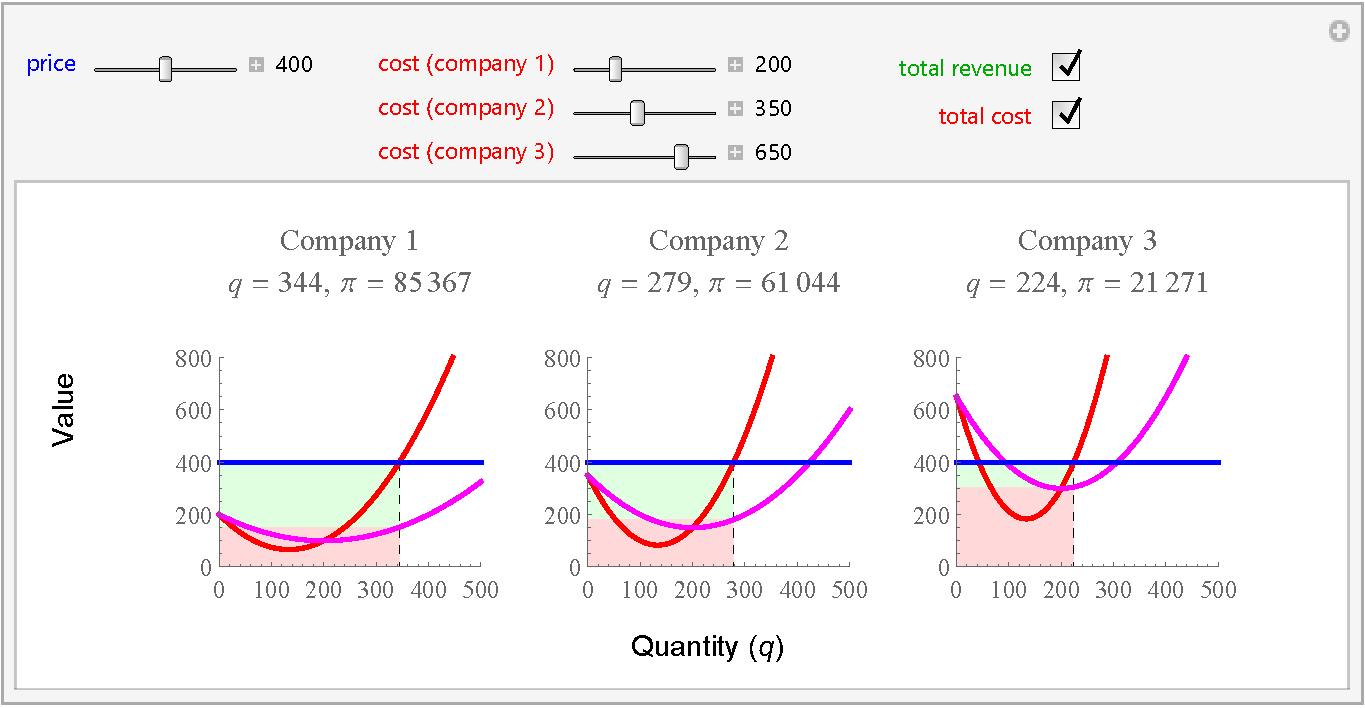
\includegraphics[width=2.8cm]{demo_IMR}}\\
\rule[10pt]{\linewidth}{.1pt}\end{remark}\end{figure}

%------------------------------------------------
\section{Pure open access equilibrium}\index{Pure open access equilibrium}\label{openaccess}
An open and unregulated fishery is often referred to as a \textit{pure open access fishery}, distinguishing between purely unregulated fisheries and fisheries which are open for all (open access fisheries) but under given, common regulations such as gear use, area restrictions, etc. See subsection~\ref{ownership} for a more precise definition.

In perfect markets (read more about perfect markets in section~\ref{perfect market}), the allocation of labour and capital will stabilise where the pay off for each normalised input factor in production is equivalent in all placements. Hence no additional gain can be obtained by moving labour and capital elsewhere. The obtained profit is referred to as normal profit, included in the total cost ($TC$) defined in Section~\ref{TC and TR}.

In a pure open access fishery we assume the single decision makers to be each unit of effort (for example each boat or each fisher) The number of decision units depends on the profitability of the fishery and the speed of entrance to and exit from the fishery. We assume all decision makers to have the same opportunity costs of labour and capital, in other word there is a given normal profit which is constant for all. We assume this normal profit also to be constant over time, as we aim to relate the open access development over time to the equilibrium model described in Section~\ref{TC and TR}. Equilibrium profit beyond the normal profit (abnormal profit) is given by Equation~\ref{eq:R} as a function of fishing effort. When considering non-equilibrium cases it is convenient to express the abnormal profit as a function of harvest. Equation~\ref{eq:schaeffer} expresses harvest as a function of two independent variables, effort ($E$) and stock size ($X$). This equation therefore also is valid outside the case of equilibrium harvest (short term harvest). According to Equation~\ref{eq:schaeffer} fishing effort is expressed by
\begin{equation} 
\label{eq:effortHX}
E = \frac{H}{q \cdot X}
\end{equation}
Inserting Expression~\ref{eq:effortHX} in Equation~\ref{eq:TC} gives the short term total cost as a function of current stock size ($X$) and harvest ($H$)
\begin{equation} 
\label{eq:shorttermTC}
TC(X,H) = \frac{a}{q \cdot X} \cdot H
\end{equation}
The first term on the right hand side is the unit cost of harvest, $c(X)$:
\begin{equation} 
\label{eq:unitcostH}
c(X) = \frac{a}{q \cdot X}
\end{equation}
Since the constant price $p$ is the unit income per harvest, short term total economic rent ($R$) now can be expressed as a function of harvest ($H$)
\begin{equation} 
\label{eq:shorttermR}
R(X,H) = \Big( p - c(X) \Big) \cdot H
\end{equation}
From Equations~\ref{eq:stockchange} we have
\begin{equation*} 
\dot{X} = f(X) - H(E, X)
\end{equation*}
$f(X)$ represents any population growth functions. In equilibrium ($\dot{X} = 0$) total economic rent is given by Equation~\ref{eq:shorttermR}
\begin{equation} 
\label{eq:RX}
R(X) = \Big( p - c(X) \Big) \cdot f(X)
\end{equation}
corresponding to Equation~\ref{eq:R}.

\begin{theorem}[Pure open access equilibrium]
\hfill \break
Equation~\ref{eq:eqharvest} is obtained directly from Equations~\ref{eq:production} and \ref{eq:schaeffer} through these steps
\begin{mmaCell}[index=1]{Input}
  f[x_] := r x (1 - x/k)
\end{mmaCell}
\begin{mmaCell}{Input}
  h[x_, e_] := q x e
\end{mmaCell}
\index{\texttt{Solve}}
\begin{mmaCell}{Input}
  x[e_] := x /. Solve[f[x] == h[x, e], x][[2]]
\end{mmaCell}
\begin{mmaCell}{Input}
  h[e_] := h[x[e], e]
\end{mmaCell}
\index{\texttt{Plot}}\index{\texttt{Evaluate}}
\begin{mmaCell}{Input}
  Plot[
    Evaluate[h[e] /. \{r -> 1, k -> 1, q -> 1\}], 
    \{e, 0, 1\}, 
    AxesLabel -> \{"Fishing effort (E)", "Equilibrium harvest (H)"\}
  ]
\end{mmaCell}
\begin{mmaCell}[moregraphics={moreig={scale=.8}}]{Output}
  \mmaGraphics{harvest}
\end{mmaCell}
Equilibrium cost and revenue are
\begin{mmaCell}{Input}
  tc[e_] := a e
\end{mmaCell}
\begin{mmaCell}{Input}
  tr[e_] := p h[e]
\end{mmaCell}
Following the definition of a pure open access fishery (average revenue equals marginal cost) the open access stock biomass ($X_\infty$) is found to be given by the price/cost ratio:
\index{\texttt{Solve}}\index{\texttt{First}}
\begin{mmaCell}{Input}
  xoa = x /. First@Solve[p h[e, x]/e == tc'[e], x]
\end{mmaCell}
\begin{mmaCell}{Output}
  \mmaFrac{a}{p q}
\end{mmaCell}
This finding makes it straight forward to identify the open access fishing effort ($E_\infty$):
\index{\texttt{Solve}}\index{\texttt{First}}
\begin{mmaCell}{Input}
  eoa = e /. First@Solve[tr[e]/e == tc'[e], e]
\end{mmaCell}
\begin{mmaCell}{Output}
  - \mmaFrac{(a - k p q) r}{k p \mmaSup{q}{2}}
\end{mmaCell}
Following the definition of a pure open access fishery (average revenue equals marginal cost)
\begin{mmaCell}{Input}
  hoa = q eoa xoa
\end{mmaCell}
\begin{mmaCell}{Output}
  - \mmaFrac{a (a - k p q) r}{k \mmaSup{p}{2} \mmaSup{q}{2}}
\end{mmaCell}
\label{code:openaccess}
\end{theorem}
In a perfect market we expect all participants to receive a normal profit (from Equation~\ref{eq:R}) after maximising their individual profit. Since each fishing unit ($u$) utilises the same biological resource ($X$) as all other units ($n$ units in total), the stock size is given. First order condition of a maximum is that marginal revenue equals marginal cost, using unit fishing effort $e_i$ as the control variable:
\begin{equation} 
\label{eq:uniteq}
p \cdot X(E) \cdot q_i = a_i
\end{equation}
under condition~\ref{eq:sumofunits} and when assuming each unit to have individual catchability coefficient ($q$) and unit cost of effort ($a$). From Equation~\ref{eq:uniteq} we can express the equilibrium stock level by the cost-price ratio
\begin{equation} 
\label{eq:apstock}
X = X(E) = \frac{a_i}{p \cdot q_i}, \quad i = \{x \in \mathbb{Z} | 1 \leq x \leq n\}
\end{equation}
When all units receive a normal profit we also have, according to Equation~\ref{eq:R}
\begin{equation} 
\label{eq:allunitseq}
p \cdot X_\infty \sum_{i=1}^{n} q_i u_i = \sum_{i=1}^{n} a_i u_i
\end{equation}
Since all vessels face the same stock level ($X_\infty = X(E_\infty)$, $E_\infty$ being the open access equilibrium fishing effort, see Code box~\ref{code:openaccess} for calculating details), according to Equation~\ref{eq:apstock} the $a_i/q_i$ relationship has to be constant for all $i$. Let us call the ratio $\rho$
\begin{equation*} 
\rho = \frac{a_i}{q_i}
\end{equation*}
giving
\begin{equation} 
\label{eq:rho}
q_i = \frac{a_i}{\rho} 
\end{equation}
which inserted into Equation~\ref{eq:allunitseq} gives this equilibrium expression for $X_\infty$
\begin{equation} 
\label{eq:allunitseq2}
X_\infty = \frac{\rho}{p}
\end{equation}
We can conclude that the fishing units may differ in scale but not in fishing efficiency. As standardised units they are all identical in the equilibrium solution. In principle they may differ when thrown out of the equilibrium (caused by external factors leading to decline or increase in the stock size), which in that case will change the profits in the different units in different ways. Those earning less than a normal profit will in the perfect market leave the fishery while those earning a profit beyond the normal level (positive economic rent) will stay and if possible increase their fishing effort. A new equilibrium solution is found when all units again obtain normal profits. Ultimately a global equilibrium solution is found for a a fleet which now has become a homogeneous fleet.

By definition fishing efficiency (technological properties) and economic performance (economic properties) are identical within the homogeneous fleet. Hence $q_i = q$ and $a_i = a$ for all $i$ and Equation~\ref{eq:uniteq} is generalised to
\begin{equation} 
\label{eq:uniteqall}
p \cdot q \cdot X(E_\infty)  = a
\end{equation}
which, also in accordance with Equation~\ref{eq:apstock}, expresses the open access equilibrium stock biomass:
\begin{equation} 
\label{eq:oax}
X_\infty = X(E_\infty) = \frac{a}{p \cdot q}
\end{equation}
Equation~\ref{eq:uniteqall} expresses the general definition of open access equilibrium; when the average revenue of the fleet ($p \cdot q \cdot X(E)$) equals the fleet's marginal cost ($a$).

Note that Equation~\ref{eq:oax} claims that the open access stock level is determined by the cost-price ratio ($a/p$) and that the biological parameters ($r$ and $K$) are not included in the expression. If the cost of fishing increases, a larger stock is needed to earn a normal profit. In the same way increased price makes it possible to earn a normal profit at a lower stock level. Also note that as long as $a > 0$ also $X_\infty > 0$. This means that in our model the stock will never go extinct as long as there are costs associated with fishing.

Unit cost of harvest is given by Equation~\ref{eq:unitcostH} as a function of stock biomass $X$. Inserting the expression for $X_\infty$ above (Equation~\ref{eq:oax}) we see that the unit cost of harvest equals the unit price $p$, confirming that the open access equilibrium indeed gives a normal profit (which is embedded in the unit cost of effort, $a$). The path towards the equilibrium solution, however, may include both positive and negative economic rent. A further analysis of this is provided in Code box~\ref{code:openaccessdynamics}.

The open access fishing effort ($E_\infty$) is found by inserting Equation~\ref{eq:oax} in Equation~\ref{eq:schaeffer}, which equals Equation~\ref{eq:eqharvest} in equilibrium, and then solving it for $E_\infty$ (when $E_\infty > 0$):
\begin{equation*} 
q \cdot \frac{a}{q \cdot p} \cdot E_\infty = q \cdot K \cdot E_\infty \Big(1- \frac{q}{r} E_\infty\Big)
\end{equation*}
\begin{equation} 
\label{eq:oae}
E_\infty = \frac{r}{q} - \frac{a \cdot r}{p \cdot q^2 \cdot K}
\end{equation}

%------------------------------------------------
\section{Open access dynamics}\index{Open access dynamics}
In the section above we have discussed the equilibrium solution of open access to a fishery given perfect markets, biological growth as a function of stock biomass and fishing effort, and a catch function which is linear in the same variables (stock biomass and fishing effort). This section deals with the dynamics leading to the equilibrium solution.

As indicated in Section~\ref{section:multispecies} fishing, in terms of modelling, represents the predator in a prey-predator relationship. Over time the stock size ($X$) and the fishing effort ($E$) vary according to the biological, the technological and the economic properties of the system. Equation~\ref{eq:verhulst} gives the $X$ an constitutes the first element of the system. How to determine the changes in the other time-variable, $E$?

According to the reasoning in Section~\ref{section:openaccess} the fishing effort is expected to increase when the profit exceeds the normal level, and decrease when the profit is below the normal profit. Let us further assume a larger change when the fifference to the normal profit is larger. The unit profit of harvest (Equation~\ref{eq:unitcostH}) indicates the levels of positive and negative differences. In addition we include a stiffness parameter, $\gamma$, which determines how fast the changes in fishing effort take place. When the $\gamma$ value is high the increase/decrease in effort i large, while it is low for small values of $\gamma$. The open access dynamics is then decribed by
\begin{equation}
\label{eq:openaccessdynamics}
\begin{aligned} & \dot{X}(t) = r \cdot X(t) \cdot \bigg(1 - \frac{X(t)}{K}\bigg) - q \cdot E(t) \cdot X(t) \\
& \dot{E}(t) = \gamma \cdot \bigg(p - \frac{a}{q \cdot X(t)}\bigg)
\end{aligned}
\end{equation}
\index{Isocline}The phaseplot of Equations~\ref{eq:openaccessdynamics} is illustrated in Figure~\ref{fig:openaccess} for a fixed $\gamma$ value ($\gamma = 0.5$). In Code box~\ref{code:openaccessdynamics} the numerical example is analysed further for different $\gamma$ values. The phaseplot provides three different illustrations of the system dynamics; isoclines, vector field and time-paths. the system has a stable equilibrium in the intersection of the two isoclines.

\begin{theorem}[Open access dynamics]
\hfill \break
We define a function \texttt{dsolve} to find the numerical solutions of the differential Equations~\ref{eq:openaccessdynamics} for given initial values of the variables ($X$ and $E$) and the stiffness parameter ($\gamma$):
\index{\texttt{NDSolve}}
\begin{mmaCell}[index=1]{Input}
  dsolve[\{e0_, x0_, \(\pmb{\gamma}\)_\}] := NDSolve[\{
    x'[t] == r x[t] (1 - x[t]/k) - q  x[t] e[t],
    e'[t] == \(\pmb{\gamma}\) * (p - a/(q x[t])),
    x[0]  == x0,
    e[0]  == e0
    \} /. values,
    \{x[t], e[t]\}, \{t, 0, 50\}
  ]
\end{mmaCell}
Apart from the stiffness parameter (which is a variable in the \texttt{dsolve} function) we assume the same parameter values as in Figure~\ref{fig:openaccess}. We place the parameter values in the list \texttt{values}:
\begin{mmaCell}{Input}
  values = \{k -> 1, r -> 1, q -> 1.5, a -> .15, p -> .5\};
\end{mmaCell}
We will explore how the stiffness parameter influences the path towards the equilibrium solution, assuming an initial unexploited stock, $X = 1$, and a low fishing effort, $E = 0.01$. We investigate three cases, $\gamma = (0.1, 0.3, 0.6)$. For each case we produce two graphs of the path over time, first placed into the $(TR, TC) - E$ axes system and the second total economic rent ($R$) over time.
\index{\texttt{Transpose}}\index{\texttt{Show}}\index{\texttt{Plot}}\index{\texttt{ParametricPlot}}\index{\texttt{GraphicsGrid}}\index{\texttt{Evaluate}}\index{\texttt{ToString}}
\begin{mmaCell}{Input}
  GraphicsGrid[Transpose[\{
    Show[\{
      Plot[
        Evaluate[\{, p*q*k*e(1 - q e/r), a e\}/.values], \{e, 0, 1\}],
      ParametricPlot[
        Evaluate[\{e[t], p*q*e[t]*x[t]\} /. values /. 
          dsolve[\{.01, 1, #\}]], \{t, 0, 50\}
        ]\}, 
        PlotRange        -> \{\{0, .85\}, \{0, .24\}\}, 
        PlotRangePadding -> None,
        Frame            -> \{\{True, False\}, \{True, False\}\},
        FrameLabel       -> \{"Fishing effort", "TR, TC, OA path"\},
        PlotLabel        -> "\(\pmb{\gamma}\) = " <> ToString[#]],
      Plot[
        Evaluate[(p*q*e[t]*x[t] - a e[t]) /. values /. 
          dsolve[\{.01, 1, #\}]], \{t, 0, 50\},
        PlotRange    -> \{-.05, .16\}, Filling -> Axis,
        FillingStyle -> \{Directive[Red, Opacity[.5]], 
          Directive[Green, Opacity[.5]]\},
        Frame        -> \{\{True, False\}, \{True, False\}\},
        FrameLabel   -> \{"Time", "R"\}, 
        PlotLabel    -> ""
      ]\} & /@ \{.1, .3, .6\}]
    ]
\end{mmaCell}
\begin{mmaCell}[moregraphics={moreig={scale=.6}}]{Output}
  \mmaGraphics{openaccess2}
\end{mmaCell}
Positive economic rent is coloured green while negative economic rent is coloured red in the plots above. All three cases converges to the equilibrium solution within the investigated fifty periods.

Which of the three cases above yields the highest economic rent? Visually the not discounted flow of economic rent over time seems to be largest in the first case (to the left). Let us include more $\gamma$ values and the case of discounting at an discount rate of ten percent.
\index{\texttt{ListLinePlot}}\index{\texttt{Table}}\index{\texttt{N} (Numeric)}\index{\texttt{Flatten}}\index{\texttt{Integrate}}\index{\texttt{Length}}
\begin{mmaCell}{Input}
  gammalist = Table[.001*i^2, \{i, 1, 10, .5\}];
  Rlist = Flatten@N[
    Integrate[(p*q*e[t]*x[t] - a e[t]), \{t, 0, 50\}] /. values /. 
      dsolve[\{.01, 1, #\}] & /@ gammalist];
  ListLinePlot[\{
    Transpose[\{gammalist, Rlist\}],
    Transpose[\{gammalist, Rlist * 
      Table[1/1.05^t, \{t, 1, Length[gammalist]\}]\}]\}, 
    Mesh        -> All, PlotRange -> \{0, All\}, 
    AxesLabel   -> \{"\(\pmb{\gamma}\)", "\(\int\)R d\(\pmb{\gamma}\)"\}, Filling -> Axis, 
    PlotLegends -> \{"Sum of R over 50 periods",
      "Sum of discounted R over 50 periods"\}
  ]
\end{mmaCell}
\begin{mmaCell}[moregraphics={moreig={scale=.6}}]{Output}
  \mmaGraphics{openaccess3}
\end{mmaCell}
Both the two curves show maximum solutions at low $\gamma$ levels, $\gamma < 0.03$, the discounted case below the other. In all cases, however, the sum is positive, reflecting the gain (also in an open access fishery) of starting a fishery on an unexploited stock.
\label{code:openaccessdynamics}
\end{theorem}

\begin{figure}[ht]
\centering
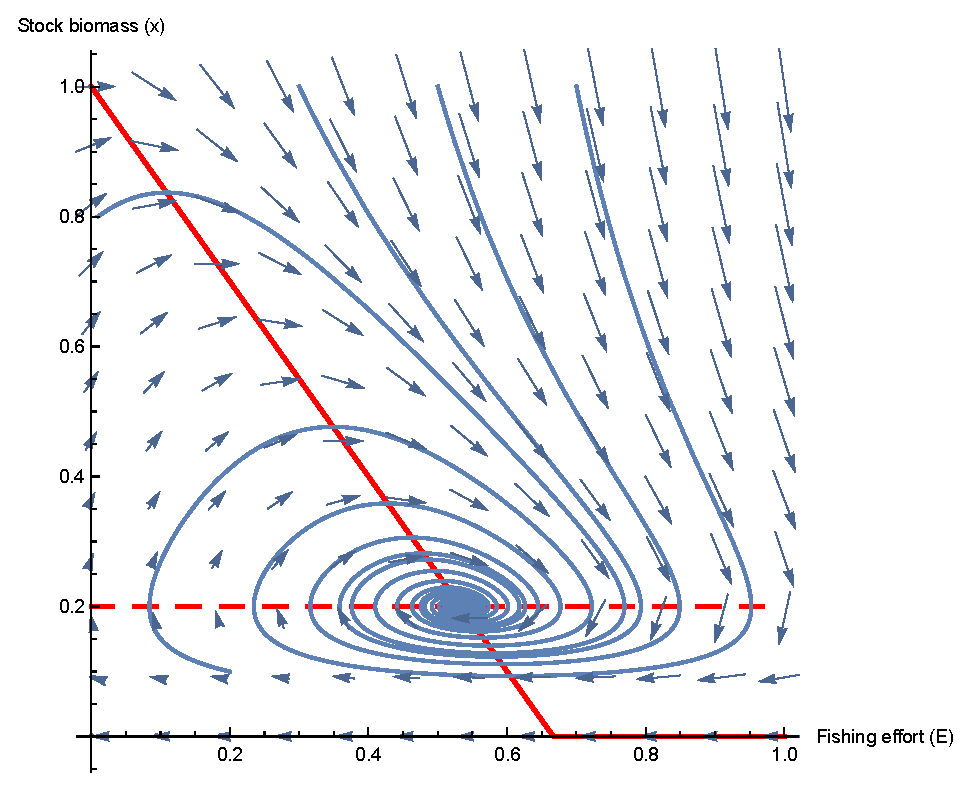
\includegraphics[scale=.8]{openaccess}
\caption{Phaseplot of a pure open access fishery as described by Equations~\ref{eq:openaccessdynamics} when $K = r = 1$, $q = 1.5$, $a = 0.15$ and $p = \gamma = 0.5$, $\gamma$ being the stiffness parameter measuring the speed at which the fleet readjust outside equilibrium. The red, dashed isocline reflects the constant stock level ($X = a/(q \cdot p)$) at which the fleet earns a normal profit. The solid, red isocline gives the equilibrium levels of the stock biomass at varying fishing effort as in Figure~\ref{fig:isocline}. The solid blue curves show paths over time toward the equilibrium point from different initial positions. The strength and direction of the dynamics in different areas are indicated by the vector field.}
\label{fig:openaccess}
\end{figure}

\begin{figure}[!htb]
\begin{remark}
\rule{\linewidth}{.1pt}
\floatbox[{\capbeside\thisfloatsetup{capbesideposition={right,top},capbesidewidth=11.8cm}}]{figure}[\FBwidth]
{\caption*{\footnotesize{Quasi rent occurs in open access dynamics and can be studied in\\the WL demonstration at 

\href{http://demonstrations.wolfram.com/QuasiRentInOpenAccessFisheries/}{\\ http://demonstrations.wolfram.com/\\QuasiRentInOpenAccessFisheries/}}}}
{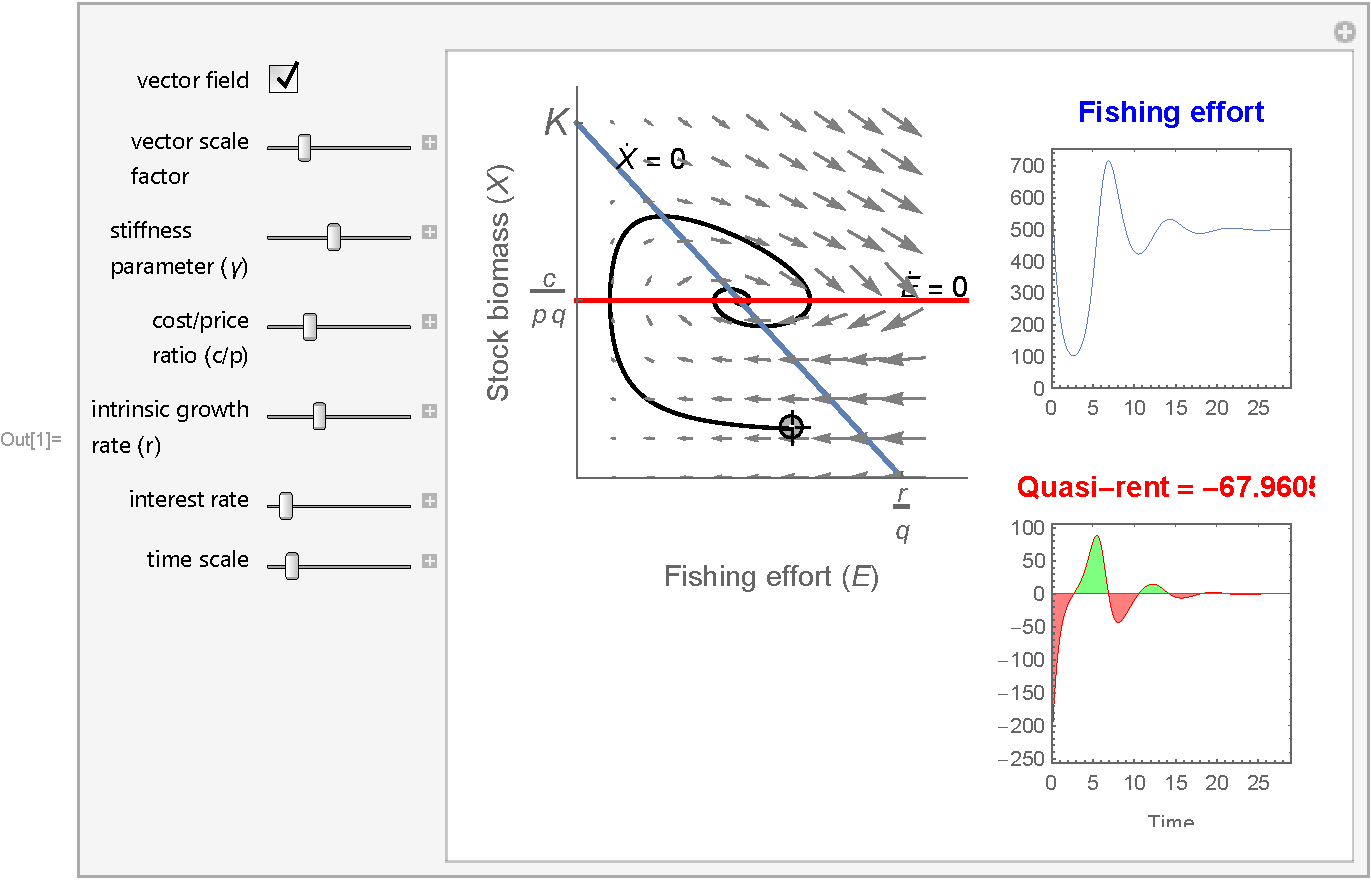
\includegraphics[width=2.8cm]{demo_OpenAccess}}\\
\rule[10pt]{\linewidth}{.1pt}\end{remark}\end{figure}

%------------------------------------------------
\section{Maximising economic rent}\index{MEY}\label{MEY}

The solution of maximising rent in equilibrium (Maximum Economic Yield, $MEY$) is straight forward when having established Equation~\ref{eq:R}. Scott Gordon\cite{Gordon1954} first published these results in 1954. The first and second order conditions of a maximum are

\begin{equation}
\label{eq:mey}
\begin{aligned} & R'(E) = TR'(E) - TC'(E) = MR(E) - MC(E) = 0\\
& R''(E) < 0
\end{aligned}
\end{equation}
$MR$ is the marginal revenue with respect of fishing effort ($E$) and $MC$ is the corresponding marginal cost of effort. The first order condition of a maximum tells that thes two should equal each other, $MR = MC$. As illustrated in Figure~\ref{fig:gordonschaefer} this occurs at the fishing effort $E_MEY$.
 
\begin{figure}[ht]
\centering
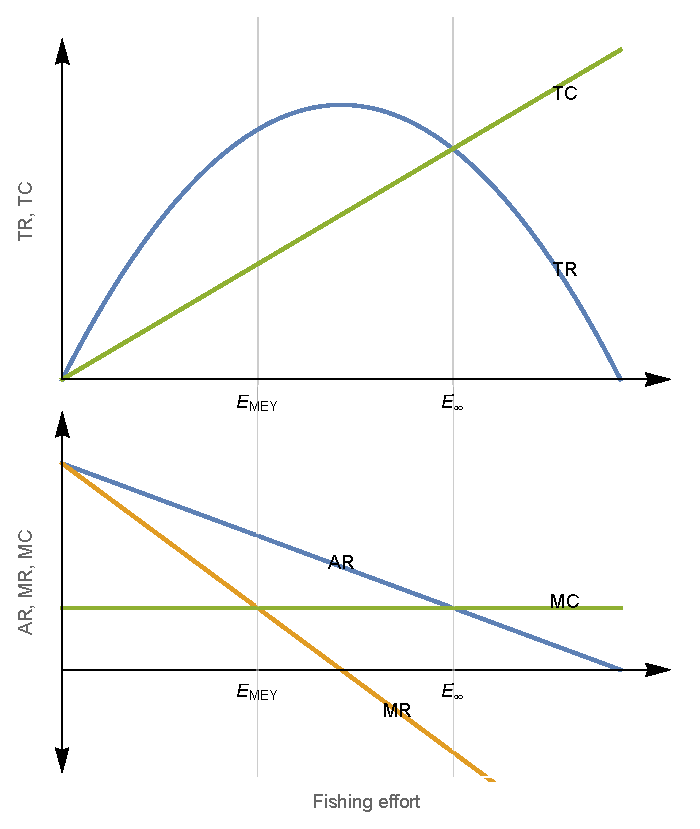
\includegraphics[scale=.9]{gordonschaefer}
\caption{The classical presentation of the Gordon-Schaefer model, on top the aggregated revenues ($TR$, blue curve) and costs ($TC$, green line) and below the marginal picture including average revenue ($AR$, blue line), marginal revenue ($MR$, orange line) and marginal cost ($MC$, green line). The equilibrium solutions for open access ($E_\infty$) and $MEY$, maximum sustainable yield ($E_{MEY}$) are indicated by the two vertical lines.}
\label{fig:gordonschaefer}
\end{figure}
\hfill \break
The idea of Maximum Economic Rent ($MEY$) was established by Scott Gordon and Anthony Scott in the mid 1950ies and several economists believed it to soon replace the biological concept of Maximum Sustainable Yield ($MSY$) which is equilibrium harvest maximisation without any references to market values.

\begin{corollary}[Talk by Anthony Scott (Bergen, 1993)] \label{highlight:scott}
\hfill \break
\small{\indent \enquote{But we should recognise now, I think, that we had been guilty of a confusing application of normative economics. All that fuss about MSY vs other targets should have stayed in the classroom, on the blackboard, for graduate students. The world had need for more of the predictions of economics, not their prescriptions, as Scott Gordon had showed. I now think we had little more business lecturing the fishing world on what they should maximise than we would have had reproving a merchant for maximising sales or a farmer for maximising his fleet of shiny new equipment. Our comparative advantage lies elsewhere. 

In any case some of us were just plain wrong-headed in our obsession with MSY. We had little or no data with which to measure the real-world difference between various optimum catches and stocks. We knew nothing about the regulatory and compliance costs attached to each optimum. We took little or no account of uncertainty, instability and irreversibility. We did not understand that the theory of the second best tended to undermine our faith in knife-edge piecemeal partial optimisation. 

We should pause to consider the moral of that chapter in the development of fishery economics. It is still embarrassing to hear a biologist of that generation say apologetically, "of course you economists believe in something entirely different". It was not that we should not have lent our talents to policy formation. Nor should we ignore welfare economics. It is that before we pooh-pooh any particular goal, or instrument for that matter, we should use our economics to predict how it will work and who it will benefit. You may not think this a very surprising conclusion in this day and age. Perhaps it is not. Nevertheless, ignoring it, we wasted a lot of everyone’s time. Our reliance on normative economics distracted us from prediction and from measurement activities where we could have done a lot of good.}}
\end{corollary}

\begin{figure}[!htb]
\begin{remark}
\rule{\linewidth}{.1pt}
\floatbox[{\capbeside\thisfloatsetup{capbesideposition={right,top},capbesidewidth=11.8cm}}]{figure}[\FBwidth]
{\caption*{\footnotesize{The Gordon-Schaefer model can be explored as a\\Wolfram Demonstration at 

\href{http://demonstrations.wolfram.com/TheGordonSchaeferModel/}{\\ http://demonstrations.wolfram.com/TheGordonSchaeferModel/}}}}
{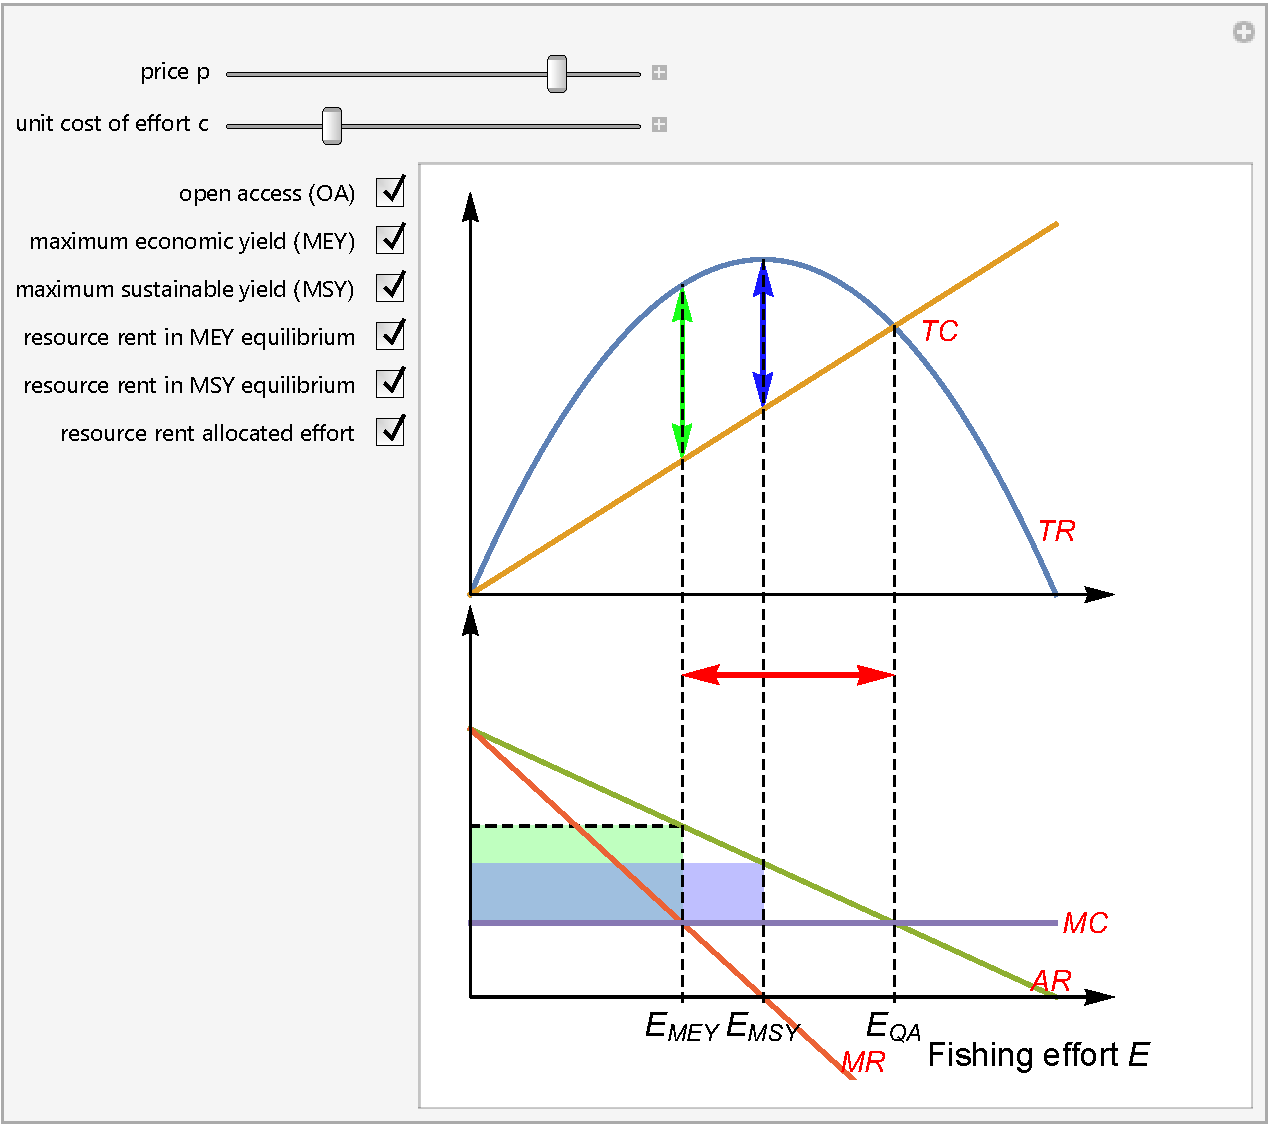
\includegraphics[width=2.8cm]{demo_GordonSchaefer}}\\
\rule[10pt]{\linewidth}{.1pt}\end{remark}\end{figure}

%------------------------------------------------
\section{Maximising present value of flow of rent over time}\index{maxPV}\label{section:pvmax}

In his textbook in fisheries economics and management Ola Flaaten presents the problem of maximising present value of fishing over time, by providing a simple example of investment\cite{Flaaten2016FisheriesManagement}. The example is a cost-benefit problem of the type: Investment or not? The investment in question is to fish one unit less or keep fishing the equilibrium catch (assuming an initial equilibrium fishery).

The complete problem is to compare the gain of fishing one unit less this time period and then establish a new equilibrium the next period, with the loss of the reduced catch this period (the investment). The latter is simply the unit profit, $p - c(X_0)$, when $X_0$ is the initial equilibrium stock size (see Equation~\ref{eq:shorttermR}). The gain is the discounted (see Code box~\ref{code:discounting}) flow of lasting difference in profits between the initial equilibrium condition and the new equilibrium. In discrete time this sum is
\begin{equation} 
\label{eq:discdiff}
 \begin{aligned} & \displaystyle\sum_{t=1}^{\infty} \frac{1}{(1+i)^t} \bigg( (p-c(X_1)) \cdot f(X_1) - (p-c(X_0)) \cdot f(X_0) \bigg) \\
 & = \bigg( (p-c(X_1)) \cdot f(X_1) - (p-c(X_0)) \cdot f(X_0) \bigg) / i \\
 & = \Big( R(X_1) - R(X_0) \Big) / i = \frac{\Delta R(X_0)}{i}
 \end{aligned}
\end{equation}
when $f(X)$ is the natural growth in stock as given as in Equation~\ref{eq:stockchange}, $R$ is total economic rent as given by Equation~\ref{eq:RX}, and $\Delta R(X_0)$ is the difference in total economic rent in equilibrium by investing one unit of harvest at time $t = 0$. The investment problem is expressed as a cost-benefit question: Is it beneficial to invest $p - c(X_0)$ (the immediate loss of fishing one unit less) when the gain is $\Delta R(X_0)/i$? Obviously the answer is yes if
\begin{equation*} 
 \frac{\Delta R(X_0)}{i} > p - c(X_0)
\end{equation*}
and the investment is not beneficial if
\begin{equation*} 
 \frac{\Delta R(X_0)}{i} < p - c(X_0)
\end{equation*}
When the immediate loss of fishing one unit more equals the long term discounted gain over all future of fishing one unit less today, the investor is indifferent between investing or not.

\begin{theorem}[Discounting] \index{Discounting}
\hfill \break
Discounting is a method of reflecting intertemporal preferences in terms of values. Since most of us prefer receiving a given value (for example 100\euro) sooner (for example now) than later (for example in ten years from now), there will exist a value to be received in the future (in our case more than 100\euro \ ten years from now) that corresponds to receiving the value now.

If we assume that the value diminishes by $100 i$ percent per year it is postponed into the future, the \textit{present value}\index{Present value} ($PV$) of 100\euro \ received ten years from now is
\begin{equation*} 
 PV = \frac{100}{(1 + i)^{10}}
\end{equation*}
Or in general, let \texttt{x} be the value in $t$ years from now representing the present value of today.
\begin{equation*} 
 PV = \frac{x}{(1 + i)^t}
\end{equation*}
Returning to our initial problem, to find the $x$-value corresponding to a present value equal 100, we have
\index{\texttt{Solve}} \index{\texttt{Simplify}}\index{\texttt{Exp}}\index{\texttt{Log}}\index{\texttt{Plot}}\index{\texttt{Show}}\index{\texttt{Limit}}\index{\texttt{D} (Derivative)}
\begin{mmaCell}[index=1]{Input}
  Solve[100 == x*(1 + i)^-10, x]
\end{mmaCell}
\begin{mmaCell}{Output}
  \big\{\big\{x \(\to\) 100\mmaSup{(1 + i)}{10}\big\}\big\}
\end{mmaCell}
We see that for each positive value of \texttt{i} there is a corresponding value of \texttt{x} larger than 100. Consider the case of 10\% discounting (\texttt{i = 0.1})
\begin{mmaCell}{Input}
  \% /. \{i -> .1\}
\end{mmaCell}
\begin{mmaCell}{Output}
  \{\{x \(\to\) 259.374\}\}
\end{mmaCell}
This tells us that given an annual discount rate of ten percent we are indifferent between receiving 100\euro \ today or about 260\euro \ in ten years from now. With a discount rate of ten percent the present value of 260\euro \ in ten years from now is 100\euro; or: The \textit{future value}\index{Future value} ten years into the future of 100\euro \ today is 260\euro.

So far we have consider cases where we calculate year by year. Such step by step calculations are referred to as \textit{discrete time} calculations. The discount term in such calculations are $(1 + i)^t$ or $(1 + i)^{-t}$ (depending on if we are calculating future or present values).

In continuous time the corresponding discount term is $e^{\delta t}$ or $e^{^-\delta t}$, again depending on if we are considering future or present values. We have used two different symbols for discrete time and continuous time discount rates, $i$ and $\delta$, respectively. Let us investigate how the two relate to each other. First find the limit value of the time derivative of the discrete time expression and let time go towards zero
\begin{mmaCell}{Input}
  Limit[D[(1 + i)^-t, t], t -> 0]
\end{mmaCell}
\begin{mmaCell}{Output}
  -Log[1 + i]
\end{mmaCell}
Then, let us take the time derivative of the continuous time discount term and find the limit when time approaches zero
\begin{mmaCell}{Input}
  Limit[D[Exp[-\(\pmb{\delta}\) t], t], t -> 0]
\end{mmaCell}
\begin{mmaCell}{Output}
  -\(\delta\)
\end{mmaCell}
If the two marginal expressions above should equal each other, we have
\begin{mmaCell}{Input}
  Simplify[Solve[-Log[1 + i] == -\(\pmb{\delta}\), i], Assumptions -> {\(\pmb{\delta}\) >= 0}]
\end{mmaCell}
\begin{mmaCell}{Output}
  \big\{\big\{i \(\to\) - 1 + \mmaSup{e}{\(\pmb{\delta}\)}\big\}\big\}
\end{mmaCell}
As seen in the plots below the difference between the two increases by the value of the discount rate. However, within fairly realistic ranges of the discount rate (as indicated in the last figure) the deviation between discrete and continuous time discounting is small.
\begin{mmaCell}{Input}
  Plot[\{\(\pmb{\delta}\), -1 + Exp[\(\pmb{\delta}\)]\}, \{\(\pmb{\delta}\), 0, 1\}, 
    PlotTheme        -> "Detailed", 
    AspectRatio      -> 1.8, 
    PlotRangePadding -> None
  ]
\end{mmaCell}
\begin{mmaCell}[moregraphics={moreig={scale=.7}}]{Output}
  \mmaGraphics{discounting1}
\end{mmaCell}
\begin{mmaCell}{Input}
  Show[\%, 
    PlotRange   -> \{\{0, .2\}, \{0, .2\}\}, 
    AspectRatio -> 1
  ]
\end{mmaCell}
\begin{mmaCell}[moregraphics={moreig={scale=.7}}]{Output}
  \mmaGraphics{discounting2}
\end{mmaCell}
Let us now consider a discounted flow of a fixed value over time. In the discrete time case we have a infinite geometric series
\begin{equation*} 
  \sum_{t=1}^{\infty} \frac{1}{(1 + i)^t} = \frac{1}{1+i} + \frac{1}{(1 + i)^2} + \frac{1}{(1 + i)^3} + \frac{1}{(1 + i)^4} + \dots + \frac{1}{(1 + i)^n} + \dotsb
\end{equation*}
when the fixed value is $1$ and the discount rate is $i$ ($i > 0$), summing from $t = 1$ to $t = \infty$. \textit{Mathematica} easily finds the sum
\begin{mmaCell}{Input}
  Sum[(1 + i)^-t, \{t, 1, Infinity\}]
\end{mmaCell}
\begin{mmaCell}{Output}
  \mmaFrac{1}{i}
\end{mmaCell}
The corresponding value when using continuous time discounting is the integral of the continuous time discount term, $e^{-\delta t}$, which gives
\begin{mmaCell}{Input}
  Integrate[Exp[-\(\pmb{\delta}\) t], \{t, 0, Infinity\}, Assumptions -> \{\(\pmb{\delta}\) > 0\}]
\end{mmaCell}
\begin{mmaCell}{Output}
  \mmaFrac{1}{\(\pmb{\delta}\)}
\end{mmaCell}
Note that the expression above is the integral from $t = 0$ (not from $t = 1$ as above) to $t = \infty$.
\label{code:discounting}
\end{theorem}

It is straight forward to convert the discrete time investment solution to continuous time. The solution of Equation~\ref{eq:discdiff} is the derivative of $R$ with respect of $X$ and the investment is $R(X)/f(X)$. Indifference between investing or not is when
\begin{equation} 
\label{eq:cbinvest}
 \frac{R'(X)}{\delta} = \frac{R(X)}{f(X)}
\end{equation}
when $\delta$ is the continuous time discount rate. Figure~\ref{fig:maxPV} shows how three reference points are defined by this expression. When the right hand side of Equation~\ref{eq:cbinvest} equals zero (when $p = c(X)$) no economic rent is earned in equilibrium. This is the bioeconomic equilibrium. The left hand side of the same equation is zero when the marginal total economic rent is zero. Since the second order derivative of R is negative R is maximised at this point. $R'(X) = 0$ for $X = X_MEY$.

\begin{figure}[ht]
\centering
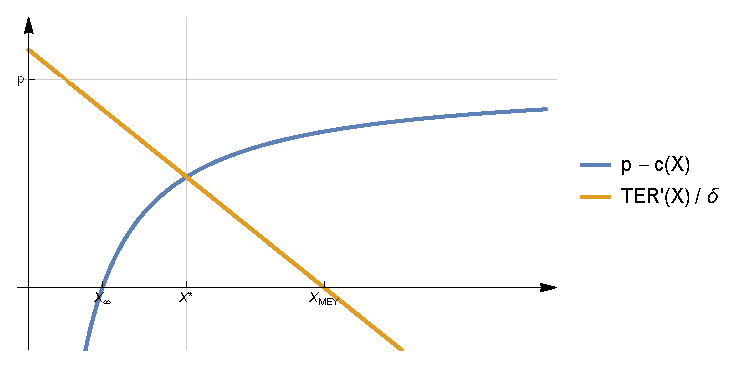
\includegraphics[scale=1.1]{maxPV}
\caption{Graphical illustration of Equation~\ref{eq:cbinvest}, showing the point that maximises present value (at $X = X^*$) as the intersection between the right hand expression of the equation, $p - c(X)$, and the left hand expression, $R'(X)/\delta$.}
\label{fig:maxPV}
\end{figure}
\hfill \break
Inserting $R(X)$ (Equation~\ref{eq:RX}) and calculating out gives the following equilibrium condition of present value maximisation:
\begin{equation} \index{Golden Rule}
\label{eq:goldenrule}
 f'(X) - \frac{c'(X) \cdot f(X)}{p - c(X)} = \delta
\end{equation}
The condition is often referred to as the Golden Rule. The Golden Rule is confirmed by employing the Euler equation on the problem. The Euler equation for equations of the type $g(t, x, \dot{x})$ (which are concave in $(x, \dot{x})$) gives the first order condition of a maximum of
\begin{equation*} 
\label{eq:euler1}
 \int_{t0}^{t1} g(t,x,\dot{x})\, \mathrm{d}t
\end{equation*}
to be given by
\begin{equation} 
\label{eq:euler2}
\frac{\partial g(t,x,\dot{x})}{\partial x} = \frac{\partial }{\partial t} \bigg( \frac{\partial g(t,x,\dot{x})}{\partial \dot{x}} \bigg)
\end{equation}
In the case of our fisheries model (equation~\ref{eq:RX}) we want to maximise the present value ($PV$) of the flow of annually discounted rent:
\begin{equation} 
\label{eq:euler3}
PV = \int_{0}^{\infty} pv(t,X,\dot{X}) \, \mathrm{d}t
\end{equation}
While assuming a discount rate equal $\delta$, $pv$ is
\begin{equation} 
\label{eq:euler4}
 pv(t,X,\dot{X}) = \Big(p - c(X) \Big) \cdot \Big(f(X) - \dot{X} \Big) \cdot e^{-\delta t}
\end{equation}
We find the left hand side of Expression~\ref{eq:euler2} to be
\begin{equation} 
\label{eq:euler5}
\frac{\partial pv(t,X,\dot{X})}{\partial X} = \bigg(f'(X) \cdot \Big(p - c(X) \Big) - c'(X) \cdot \Big(f(X) - \dot{X} \Big) \bigg) \cdot e^{-\delta t}
\end{equation}
Similarly the right hand side of Expression~\ref{eq:euler2} is found by taking the $\dot{x}$- and time-derivative of Equation~\ref{eq:euler4}:
\begin{equation} 
\label{eq:euler6}
\frac{\partial }{\partial t} \bigg( \frac{\partial pv(t,X,\dot{X})}{\partial \dot{X}} \bigg) = \delta \cdot \Big( p - c(X) \Big) \cdot e^{-\delta t} 
\end{equation}
Since $PV$ is maximised when Equation~\ref{eq:euler5} equals Equation~\ref{eq:euler6} we get this equilibrium ($\dot{X} = 0$) condition for maximum
\begin{equation*} 
\label{eq:euler8}
\bigg(f'(X) \cdot \Big(p - c(X) \Big) - c'(X) \cdot (f(X) \bigg) \cdot e^{-\delta t} = \delta \cdot \Big( p - c(X) \Big) \cdot e^{-\delta t}
\end{equation*}
\begin{equation*} 
 f'(X) - \frac{c'(X) \cdot f(X)}{p - c(X)} = \delta
\end{equation*}
As we see Equation~\ref{eq:goldenrule} is then formally confirmed.

\index{Golden Rule}The Golden Rule (Equation~\ref{eq:goldenrule}) provides a useful interpretation of the optimal solution. The right hand side, the discount rate $\delta$, is the pay off received in the best alternative placement of the natural capital, while the left hand side gives the pay off received by natural growth, adjusted for net extraction cost. If the cost is zero, $c(X) = 0$, also $c'(X) = 0$, hence $f'(X) = \delta$ (see figure~\ref{fig:optnocost}). In this case the optimal equilibrium is obtained at the stock size where the marginal biological growth, $f'(X)$, equals the discount rate. Since $f'(X) > 0$ only when $X < X_MSY$, the optimal solution when $c(X) = 0$ and $\delta > 0$ will always result in a biologically overexploited resource.
\begin{figure}[ht]
\centering
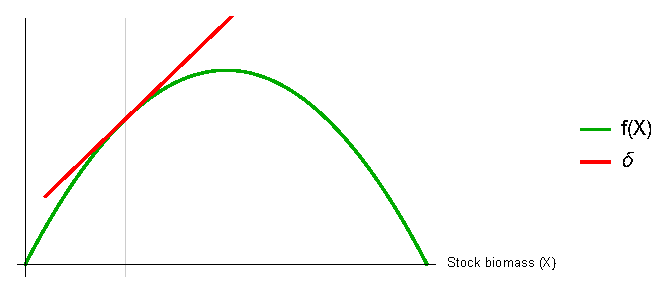
\includegraphics[scale=1.1]{optnocost}
\caption{In case of no cost ($c(X) = 0$) optimal equilibrium is obtained in the point where $f'(X) = \delta$. Here the discount rate ($\delta$) equals the slope of the red line.}
\label{fig:optnocost}
\end{figure}
\hfill \break
For $c(X) > 0$ (the normal case) the value of the left hand side of Equation~\ref{eq:goldenrule} will increase compared with the situation above, since $c'(X) < 0$ (see Equation~\ref{eq:unitcostH}). In this case, negative values of $f'(X)$ are possible solutions (which means that $X > X_MSY$), depending on the price-cost-ratio. The impact the cost equation ($c(X)$) has therefore suggests larger stocks, while the growth properties of the stock (particularly when assuming compensation growth) favour lower stock size. The final result becomes a trade-off between the two forces, as expressed in Equation~\ref{eq:goldenrule}.

\begin{figure}[!htb]
\begin{remark}
\rule{\linewidth}{.1pt}
\floatbox[{\capbeside\thisfloatsetup{capbesideposition={right,top},capbesidewidth=11.8cm}}]{figure}[\FBwidth]
{\caption*{\footnotesize{Investigate the differences between\\discrete and continuous time discounting at

\href{http://demonstrations.wolfram.com/ContinuousAndDiscreteTimeDiscounting/}{\\ http://demonstrations.wolfram.com/ \\ ContinuousAndDiscreteTimeDiscounting/}}}}
{\includegraphics[width=2.8cm]{demo_Discounting}}\\
\rule[10pt]{\linewidth}{.1pt}
\end{remark}
\end{figure}

%------------------------------------------------
\section{Optimal control theory}\index{Optimal control theory}\index{Golden Rule}

In Section~\ref{section:pvmax} we found the condition referred to as the Golden Rule. This condition has to be satisfied while identifying the equilibrium that maximises the sum of discounted economic rent over time. The methods we have discussed so far do however not explain how to obtain this equilibrium state in an optimal way. How could the optimal path toward the optimal equilibrium be found?

In 1959 Lev Pontryagin (1908 -- 1988) published a paper presenting what was later known as the \textit{maximum principle}\cite{Desoer1961} and in 1979 Colin Clark and Gordon Munro applied the new theory on a simplified case of a fishery\cite{Clark1975} corresponding to the problem described above. From equation~\ref{eq:stockchange} we can substitute $\dot{X}(t)$ by $E(t)$ or $H(t)$, both are filling the requirements of being a \textit{control variable} of the maximisation problem. Let us consider the case of equation~\ref{eq:euler3}. The catch ($H$) is the control variable of the problem and the stock size ($X$) is the \textit{state variable}. The problem is to maximise $PV$ within the time interval $t \in [0, T]$.
\begin{equation} 
\label{eq:maxprinciple1}
max[PV] = max\Big[\int_{0}^{T} pv(t,X(t),H(t)) \, \mathrm{d}t \Big]
\end{equation}
Inserting for equation~\ref{eq:euler4} we get
\begin{equation} 
\label{eq:objectfunc}
max[PV] = max\Big[\int_{0}^{T} \Big(p - c(X(t)) \Big) \cdot H(t) \cdot e^{-\delta t} \, \mathrm{d}t \Big]
\end{equation}
The expression is maximised subject to the stock's biological growth constraint (equation~\ref{eq:stockchange}):
\begin{equation*} 
\dot{X} = f(X) - H
\end{equation*}
Equation~\ref{eq:objectfunc} and the constraint above are expressed in a \textit{Hamiltonian equation}, representing a conventional way of solving this type of problems
\begin{equation} 
\label{eq:hamiltonian}
\mathcal{H} = \Big(p - c(X) \Big) \cdot H \cdot e^{-\delta t} + \lambda(t) \big( f(X) - H\big)
\end{equation}
The optimal catch, $H$, is the catch maximising the Hamiltonian for all $t \in [0, T]$. We assume $H \in [0, H_{max}]$). 

Similarly to a Lagrange equation, the constraint of the problem (in our case the stock constraint) is represented by the last term where $\lambda$ appears. While $\lambda$ is a constant in the Lagrange equation it is a function of time, $t$ in the Hamiltonian, since our constraint now is expressed as a differential equation. $\lambda(t)$ is often referred to as the adjoint or costate variable\cite{Clark1975}. 

If $H$ does not constrain the maximisation problem, we have the following necessary conditions of a maximum
\begin{equation} 
\label{eq:optcondition1}
\frac{\partial \mathcal{H}}{\partial H} = 0
\end{equation}\begin{equation} 
\label{eq:optcondition2}
\frac{\partial \mathcal{H}}{\partial X} = - \frac{d \lambda}{d t}
\end{equation}
All pairs of $H(t)$ and $X(t)$ that satisfy this two conditions for $t \in [0, T]$ describe the optimal path towards $H(T)$ and $X(T)$.

\begin{theorem}[The Maximum Principle] \index{Maximum principle}
\hfill \break
The Hamiltonian is given as a function of the state variable $X$ and the control variable $H$ in equation~\ref{eq:hamiltonian}:
\index{\texttt{Solve}} \index{\texttt{D} (Derivative)} \index{\texttt{FullSimplify}}\index{\texttt{Exp}}
\begin{mmaCell}[index=1]{Input}
  hamiltonian[x_, h_] := (p - c[x]) h Exp[-\(\pmb{\delta}\) t] + \(\pmb{\lambda}\)[t](f[x] - h)
\end{mmaCell}
According to condition~\ref{eq:optcondition1} The derivative of \texttt{hamiltonian} with respect of the control variable \texttt{h} equals zero. We solve the equation for \texttt{$\lambda$[t]}:
\index{\texttt{D} (Derivative)}\index{\texttt{Solve}}
\begin{mmaCell}{Input}
  lamda[tt_, xx_] := (\(\pmb{\lambda}\)[t] /. Solve[
        D[hamiltonian[x, h], h] == 0, \(\pmb{\lambda}\)[t]
      ][[1]]) /. \{t -> tt, x -> xx\}
\end{mmaCell}
Then we have the definition
\begin{mmaCell}{Input}
  lamda[t, x]
\end{mmaCell}
\begin{mmaCell}{Output}
  \mmaSup{\(e\)}{-t \(\pmb{\delta}\)} (p - c[x])
\end{mmaCell}
The economic interpretation of this term is straight forward and easily understood when looking at the expression: The shadow price of one unit of harvest at time \texttt{t} is the discounted unit economic rent. The time derivative of the shadow price is
\index{\texttt{D} (Derivative)}\index{\texttt{FullSimplify}}
\begin{mmaCell}{Input}
  D[lamda[t, x[t]], t] // FullSimplify 
\end{mmaCell}
\begin{mmaCell}{Output}
  -\mmaSup{\(e\)}{-t \(\pmb{\delta}\)} (p \(\pmb{\delta}\) - \(\pmb{\delta}\) c[x[t]] + c'[x[t]] x'[t])
\end{mmaCell}
According to condition~\ref{eq:optcondition2} the derivative of the Hamiltonian with respect of the state variable equals minus the time derivative of $\lambda$. We use this condition to find an expression for $\lambda$:
\index{\texttt{D} (Derivative)}\index{\texttt{FullSimplify}}\index{\texttt{Solve}}
\begin{mmaCell}{Input}
  Solve[
    -D[hamiltonian[x[t], h], x[t]] == D[lamda[t, x[t]], t], \(\pmb{\lambda}\)[t]
  ][[1]] // FullSimplify
\end{mmaCell}
\begin{mmaCell}{Output}
  \Big\{\(\pmb{\lambda}\)[t] \(\to\) \mmaFrac{\mmaSup{\(e\)}{-t \(\pmb{\delta}\)}(p \(\pmb{\delta}\) - \(\pmb{\delta}\) c[x[t]] + c'[x[t]](h + x'[t]))}{f'[x[t]]}\Big\}
\end{mmaCell}
We now have two expressions of $\lambda$ that should be equal:
\index{\texttt{FullSimplify}}\index{\texttt{Solve}}
\begin{mmaCell}{Input}
  Solve[(\(\pmb{\lambda}\)[t] /. \%) == lamda[t, x[t]], \(\pmb{\delta}\)][[1]] // FullSimplify 
\end{mmaCell}
\begin{mmaCell}{Output}
  \Big\{\(\pmb{\delta}\) \(\to\) f'[x[t]] - \mmaFrac{c'[x[t]] (h + x'[t])}{p - c[x[t]]}\Big\}
\end{mmaCell}
\index{Golden Rule}
The solution is found to be equal to the Golden Rule (equation~\ref{eq:goldenrule}) since \\
$\texttt{(h + x'[t]) = f[x]}$ (as given by equation~\ref{eq:stockchange}). Hence, the only pair of \texttt{x} and \texttt{h} fulfilling the requirement given above is the equilibrium solution referred to as the Golden Rule (optimal equilibrium). Consequently a \textit{bang-bang-solution}\index{Bang-bang-solution} represents the optimal path towards the optimal equilibrium ($X^*, H^*$):
\begin{equation*} 
H_{opt} = \left\{ \begin{array}{lcl}
0       & \mbox{for} & X < X^* \\ 
H_{max} & \mbox{for} & X > X^* \\
H^*     & \mbox{for} & X = X^*
\end{array}\right.
\end{equation*}
given that $H \in [0, H_{max}]$ and $0 < H^* < H_{max}$.
\label{code:maximumprinciple}
\end{theorem}
%------------------------------------------------
\section{Why do we observe fleet diversity?}\index{Fleet diversity}

Given the reasoning above we should only find one type of vessels, namely the most cost efficient type, in all fisheries that have been open for all to participate. As open access has been the normal situation until quite recently in most fisheries, we should expect to find homogeneous fleets most places. This does however not to be the case. Then why should we find diverse fleets when the theory seems to predict the opposite?

This question may turn out to quite essential for our understanding of the equilibrium model and the limits it has. Since a diverse fleet structure seems to be the situation in most fisheries we have to possible conclusions: 1) Something in the equilibrium models we have been discussing is wrong, or 2) Equilibrium is a theoretical concept and is never achieved in real world fisheries.

The first conclusion can perhaps not be fully rejected. As discussed in section~\ref{goodmodel} models cannot be true, but they may be useful or not. Let us therefore look at the other conclusion. Is it possible to claim the equilibrium concept and the models based on this still to be useful, even when an equilibrium situation is never established?

MORE TO COME

%------------------------------------------------
\section*{Exercises}\index{Exercises!Chapter 6}
\addcontentsline{toc}{section}{Exercises}

\begin{exercise}
Why increases the production more rapidly in the lower-right figure in Code box~\ref{code:expansionpaths} than in the upper-right figure?
\end{exercise}
\begin{exercise}
What is the unit cost of a product following a Cobb-Douglas production process and economic efficient use of input factors when the output elasticities equal one?
\end{exercise}
\begin{exercise}
Prove that output eight (\texttt{Out[8]}) in Code box~\ref{code:discounting} is correct.
\end{exercise}


\chapterimage{h7.jpg} % Chapter heading image

%------------------------------------------------
\chapter{Fisheries and markets} \label{chapter 7}
%----------------------------------------------------------------------------------------
%	CHAPTER 7
%----------------------------------------------------------------------------------------

%------------------------------------------------
Commercial fisheries need market places to sell the catches to prices by which they can at least cover the cost of fishing. As discussed in chapter~\ref{chapter 1} there are market challenges related to sale of perishable goods, as for example fresh fish. The development of preservation methods has contributed in increasing the seafood trade. Seafood production and trade today has become a major global industry.

%------------------------------------------------
\section{The global seafood market}\index{The global seafood market}\label{seafood market}
Seafood production and trade have gone through significant changes after the second world war. In 1950, the year \index{FAO!Code of Conduct}The Food and Agriculture Organisation of the United Nation (FAO) started to register fish harvest globally, the world catches summed up to 16.5 million tons (see figures~\ref{fig:worldcatches1} and \ref{fig:worldcatches2}). The global catches increased year by year up to the mid eighties and since then it has stabilised on around 70 -- 80 million tons each year.

\begin{figure}[ht]
\centering
\includegraphics[scale=.97]{continentcatch}
\caption{Global fish catches in 1950, 1975, 1995 and 2015 retrieved from the \href{http://www.fao.org/fishery/topic/16140/en}{FAO online data base (http://www.fao.org/fishery/topic/16140/en)}, separated on continents of the fishing nations.}
\label{fig:worldcatches1}
\end{figure}

Global catches have been stable over a period of more than thirty years but the distribution of catches shows interesting patterns over time. While Europe and the Americas (South- and North-America) stood for 2/3 of the catches in the 1950ies, the share in 2015 was about 1/3 and total global catch was five times larger than in 1950 (see figure~\ref{fig:worldcatches1}). This is also reflected in figure~\ref{fig:worldcatches2} where the global catches are distributed on three levels of economic development. In 1950 about 3/4 was caught by economically developed countries while the share in 2015 was about 1/4. We also see from figure~\ref{fig:worldcatches2} that the changes first of all happened after 1975, which coincides with the introduction of Exclusive Economic Zones (see chapter~\ref{chapter 9}). 

\begin{figure}[ht]
\centering
\includegraphics[scale=.97]{economiccatch}
\caption{Global fish catches in 1950, 1975, 1995 and 2015 retrieved from the FAO online data base at \href{http://www.fao.org/fishery/topic/16140/en}{http://www.fao.org/fishery/topic/16140/en}, separated on economic state of the fishing nations.}
\label{fig:worldcatches2}
\end{figure}

Today seafood (and certainly when including aquaculture production) is the single most important commodity offered by developing countries in a global market\cite{FoodandAgricultureOrganizationoftheUnitedNations.FisheriesandAquacultureDepartment2018} and it is becoming increasingly more important for the least developed economies. Compared with other typical commodities traded from developing countries (agriculture products like fruit, tobacco, cacao, etc.) the prices on seafood products in general are kept relatively high in international markets, compared with other products originating from developing countries. This may reflect that international demand has increased more than the corresponding supply of such products. It should be noted that figures~\ref{fig:worldcatches1} and \ref{fig:worldcatches2} reflect total global catches, not trade. However, most of the global fish catches are traded in international markets.

\begin{figure}[ht]
\centering
\includegraphics[scale=.36]{continentimport}
\caption{Global fish and fish products imports on continents in 2016 in terms of value, retrieved from \href{javascript:new_window(http://www.fao.org/documents/card/en/c/I9540EN)}{FAO's SOFIA report of 2018 (pages 58--59)}. The imported shares of total imports to each continent are indicated by digits, import from own continent is also included.}
\label{fig:worldcatches3}
\end{figure}

Figure~\ref{fig:worldcatches3} shows the shares of values of imported fish and fish products distributed on continents. 63\% of the imported fish in Oceania and 48\% in North-America come from Asia, while European fish products make up 19\% of the Asian import and 37\% of the African import. Note that it is only in Europe, Asia and South-America the internal trade is equal or surpasses the import from other continents. The internal trade within one continent is however closely linked to the number of countries at the continent.

\begin{figure}[ht]
%\centering
\flushleft
\includegraphics[scale=.52]{fishconsumption}
\caption{Global fish consumption distributed on continents in 2016, giving the population size along the horizontal axis and the fish consumption per capita along the vertical axis. The data is from \href{javascript:new_window(http://www.fao.org/documents/card/en/c/I9540EN)}{FAO's SOFIA report of 2018 (Table 18 on page 72).} Total fish consumption of each continent is shown in the centre of each box in million tons.}
\label{fig:worldcatches4}
\end{figure}

\begin{figure}[ht]
%\centering
\flushleft
\includegraphics[scale=.52]{fishconsumption2}
\caption{Global fish consumption distributed on economies in 2016, giving the population size along the horizontal axis and the fish consumption per capita along the vertical axis. The data is from \href{javascript:new_window(http://www.fao.org/documents/card/en/c/I9540EN)}{FAO's SOFIA report of 2018 (Table 18 on page 72).} Total fish consumption of each economy is shown in the centre of each box in million tons.}
\label{fig:worldcatches5}
\end{figure}

Figures~\ref{fig:worldcatches4} and \ref{fig:worldcatches5} show the world consumption of fish products in 2016, with respect of the distribution on continents and and the distribution on economies. In average one individual in South-America and Africa consume about 10 kilo per year, while the corresponding consumption on the other continents is more than double. Figure~\ref{fig:worldcatches5} shows that there are significant differences depending on economic state, which also explains the modest fish consumption in South-America and Africa. Only the tiny population in Oceania consumes somewhat more per individual that the Asian population does. About half of the fish consumption in 2016 came from aquaculture production.

%------------------------------------------------
\section{Market failures}\index{Market failures}\label{perfect market}
In a perfect market the price is determined where the demand meets the supply of the good, all share the same information and no parts have market power, which is the ability to influence the price formation alone. This idealised situation is rare but on the other hand, often the price formation will lead to prices close to those we would find in perfect markets. One think about the market solution as the result of a negotiation between consumers (demand) and suppliers where the correct price is found when no part could increase or decrease the price without loosing.

\begin{figure}[ht]
\centering
\includegraphics[scale=.62]{perfect_market}
\caption{The market cross, the intersection between demand and supply, really is one point, $(Q_p, p)$, in the intersection between two areas: The area of acceptance from the supply side, and the area of willingness to pay from the demand side. The horizontal axis gives the quantity produced and the vertical axis the unit price of the good.}
\label{fig:perfectmarket}
\end{figure}

Market failure is caused by factors disturbing the market solution displayed in figure~\ref{fig:perfectmarket}. External factors (externalities), reflected in costs not payed for by the producer, hinder perfect market solutions to be obtained. Perfect market solutions may also be altered by governmental regulations where the authorities search to avoid free market solutions.

In some of the Nordic countries the government has introduced monopolies on the supply side, deliberately aiming to reduce the quantities sold (e.g. liqueur monopolies) or provide the supply side with monopoly profits (as in the case of regulations of the taxi market, believing that a profit beyond normal level will contribute in making the service more safe for the public).

In other cases market failure is unintended, as in case of polluting industries not including the damage caused by the pollution in the cost of production. When some of the cost of production is omitted by the producer (by forwarding it to the society) it is not reflected in the supply curve (figure~\ref{fig:perfectmarket}) and the price becomes too low and the quantity too high, compared with including the external cost. the market failure here cause too high production, while it in the case of governmentally introduced monopolies is produced less than in perfect markets.

The first-hand market of fish (when catch is transferred from fisher to fish-buyer) may also be imperfect. As you can read from Additional remark~\ref{highlight:rawfishact}, the fishers (or rather the fishers sales organisation) can dictate -- within certain constraints -- the first-hand price of fish in Norway. One of the motivations of this is to avoid the fish-buyers to take advantage of their potential market power. The aim is not to provide the fishers with more market power than the buyers, but to level this out. Both parts then has to share the responsibility of finding an efficient price.

%------------------------------------------------
\begin{corollary}[The Norwegian \textit{Raw Fish Act}] \label{highlight:rawfishact}
\hfill \break
\small{\indent Fishers usually do not sell fish directly to consumers. When fish is landed it usually goes to a fish buyer and there may be several additional chains until the final product reaches the consumer. The product may be processed in a number of ways before it finally is consumed. However, in modern fish trade the product could end up in a store on a different continent after relatively short time. Nevertheless, the price obtained by the fishers may still appear to be rather disconnected from the final price the consumer has to pay. The value chain from catch to consumption is an interesting study of its own but it falls outside the scope of this book. Our interest is the harvest and related subject, including the price the fisher obtain when selling the fish in a port. We refer to this market as \textit{the first-hand market}.

The nature of fishing makes it difficult to organise fishers to operate coordinated in the first hand market. Traditionally the fisher therefore has been the weaker part in price bargaining with raw fish buyers. When the fish is fresh from the sea and a price has to be negotiated, the buyer often is in a stronger position than the fisher, particularly if there are competition between many fishers in need to sell their fish before it is spoiled and a few or one buyer (\textit{monopsony}). However, the negotiation may also be influenced by possible commitments the buyers may have to their customers. There are a number of factor affecting the market relationship between fisher and buyer and in a modern fishing society the sample space of actions is controlled by laws and regulations.

In order to provide the fishers in Norway with a stronger bargaining power in the first-hand market, the so called \textit{Raw Fish Act}\index{Norwegian Raw Fish Act} passed in 1938, giving the fishers' cooperative sales-organisation the right to decide prices and conditions of this market\cite{Jentoft2018BuildingNorway}. 

The buyers had built up their market power and position within the fishing industry on the basis of privileges from the King. After the \textit{Raw Fish Act} the fishers could decide on first-hand prices, and had to take the responsibility of creating a healthy first-hand market. If the sales-organisation on behalf of the fishers set the price too high, many buyers will not be able to buy and the catches could not be sold. If the price is set too low, the fishers will lose. It was necessary to have good market information and to be flexible enough to account for geographical and other differences in every single market operation along the coast. 

The Norwegian \textit{Raw Fish Act} replaced one market failure with another. It is easy to show that situations may occur where both fisher and buyer have advantage of omitting the rules and make illegal arrangements to make it pass the regulated system. Of this reason problems of catch registration on wrong species, fixing weight measurements, etc. have been, and still are, real issues in regulated first-hand fish markets.}
\end{corollary}

There is a naturally embedded market failure in fishing since a number of individual producers (fishers) target the same stock. Every fisher has to meet the impact on the stock by the fishing activity of all fishers. Hence, there are external costs related to the fishing activity, a cost that has to be payed for by all fishers. 

Essentially this is the problem of open access fishing, as discussed in Section~\ref{openaccess}. The market failure related to external cost will disappear in the case of a sole ownership of the resource. The owner will maximise the profit without any interference from other actors, which means that the stock biomass $X$ in Equation~\ref{eq:shorttermR} indirectly is controlled by the owner's decisions.

%------------------------------------------------
\section{The problem of the sole owner}\index{The problem of the sole owner}\label{sole owner}
A resource owner is a monopolist in sense of having exclusive access to the stock resource, but does not necessarily have monopoly power in the fish market. If the resource owner is price taker (without market power in the fish market), profit maximisation of the owner will follow the idea of resource rent maximisation in Section~\ref{MEY}, as first described by Scott Gordon in 1954\cite{Gordon1954}.

Consider the case of a sole owner having market power, in the meaning of being able to influence the market price on harvest by controlling the size of the harvest, $H$. Equation~\ref{eq:RX} then modifies to           
\begin{equation} 
\label{eq:RXH}
R(X,H) = \Big( p(H) - c(X) \Big) \cdot H
\end{equation}
where both the catch $H$ and the stock size $X$ in equilibrium in the long run are determined by the fishing effort, $E$, of the sole owner. Assume that the market power of the sole owner is reflected in this inverse demand function:
\begin{equation} 
\label{eq:inversedemand}
p(H) = p_0 - s \cdot H
\end{equation}
where the two parameters ($p_0$ and $s$) both are positive constants, hence the price is a down-sloping function of harvest. Inserting Equation~\ref{eq:inversedemand} in Equation~\ref{eq:RXH} and substituting $H$ for $f(X)$, assuming an equilibrium situation (when $\dot{X} = 0$ in equation~\ref{eq:stockchange}), $f(X)$ gives the natural per period growth in the stock.
\begin{equation} 
\label{eq:RXp}
R(X) = \Big(p_0 - s \cdot f(X) - c(X) \Big) \cdot f(X)
\end{equation}
Equation~\ref{eq:RXp} is the net revenue the sole owner wants to maximise. The control variable of the sole owner is the catch, $H$, hence we take the derivative of equation~\ref{eq:RXp} with respect of $H$ and set it equal to zero:
\begin{equation} 
\label{eq:Rder}
\begin{aligned}
  \frac{d R(X)}{d X} &=  0 \\\\
  \Big(p_0 - 2 \cdot s \cdot f(X)\Big) \cdot f'(X) - c(X) \cdot f'(X) &= 0
\end{aligned}
\end{equation}
We see that it is the term $2 \cdot s \cdot f(X)$ that makes the expression in equation~\ref{eq:Rder} different from the situation we discussed in section~\ref{openaccess}. If we assume $c(X) =a/(q \cdot X)$ (equation~\ref{eq:unitcostH}) and a logistic growth function ($f(X) = r \cdot X \cdot (1 - X/K)$, being the first term of equation~\ref{eq:hverhulst}) we can express equation~\ref{eq:Rder} in this way
\begin{equation} 
\label{eq:Xsole}
\frac{r}{q K^2} \cdot \Bigg(a K + q (K - 2 X) \Big(2 r s X^2 + K (p_0 - 2 r s X) \Big) \Bigg) = 0
\end{equation}
and we see that this is an cubic equation of $X$; hence, the solution has three roots. In case the sole owner has market power (the catch production of the owner affects the first-hand price, e.g. $s > 0$) the owner takes advantage of this by reducing the production. But even if $s = 0$ and the owner is price taker, he will reduce the fishing effort compared with an open access fishery (see section~\ref{openaccess}), and take advantage of the potential resource rent in the fishery. 

In equations~\ref{eq:TC} and \ref{eq:TR} total cost ($TC$) and total revenue ($TR$) in equilibrium are explained by the variable $E$ (fishing effort). Since there is a unique relationship between $E$ and $X$ expressed in equation~\ref{eq:stockeq}, we can express $TC$ and $TR$ as functions of $X$, which we actually have done above. We have
\begin{equation} 
\label{eq:TCX}
TC(X) = c(X) \cdot f(X)
\end{equation}
and
\begin{equation} 
\label{eq:TRX}
TR(X) = p(X) \cdot f(X)
\end{equation}
assuming that there exists an equilibrium price for any stock biomass level (as we also have assumed above, where $p(X) = p_0 - s \cdot f(X)$).

\begin{figure}[ht]
\centering
\includegraphics[scale=.65]{sole_owner_market}
\caption{Graphical representation of equations~\ref{eq:TCX} and \ref{eq:TRX}, assuming the price to follow a linear function of harvest (equation~\ref{eq:inversedemand}) and a logistic biological growth. Parameter values used are: $r = 1/3$, $q = 1/24$, $K = 1800$, $a = 90$, $p_0 = 18$ and $s = 1/12$. The three solutions of the cubic function is found for $X = 549$ (local maximum of resource rent), $X = 720$ (local minimum of resource rent) and $X = 1440$ (global maximum of resource rent).} 
\label{fig:soleownermarket}
\end{figure}

\begin{figure}[ht]
\centering
\includegraphics[scale=.65]{sole_owner_net_revenue}
\caption{Graphical representation of equation~\ref{eq:RXp}, assuming the price to follow a linear function of harvest (equation~\ref{eq:inversedemand}) and a logistic biological growth as in figure~\ref{fig:soleownermarket}. Parameter values used are as in figure~\ref{fig:soleownermarket} and minimum and maximum values of net revenue are indicated.} 
\label{fig:soleownernetrevenue}
\end{figure}

In figure~\ref{fig:soleownermarket} one curve is drawn for total revenue and a line for total cost of fishing. In figure~\ref{fig:soleownernetrevenue} these two curves are summarised and the net revenue is drawn (equation~\ref{eq:RXp}) for the same parameter values as those given in figure~\ref{fig:soleownermarket}. When the latter reach positive values the sole owner has covered the cost of fishing and can earn additional rent. The supply offered by the sole owner is determined by the cost that needs to be covered. Since the cost may vary depending on the production (here: harvest), also the supply will vary by the size of harvest. As above we only consider equilibrium situations; hence, the supply curve we will identify is a collection of equilibriums. In equilibrium we have $\dot{X} = 0$ and according to equation~\ref{eq:stockchange}
\begin{equation*} 
H(X) = f(X)
\end{equation*}
which could be solved for $X$. Assuming logistic growth we get two roots:
\begin{equation} 
\label{eq:Xsol}
X = \frac{r K \pm \sqrt{K} \cdot \sqrt{r ( r K - 4 H)}}{2 r}
\end{equation}
By substituting $H$ for $X$ in equation~\ref{eq:TCX} we get the total costs expressed with the variable $H$. The marginal cost per unit of harvest then is found as the derivative of the new expression. We get
\begin{equation*} 
\frac{d TC}{d H} = \pm \frac{a r}{q \sqrt{K} \cdot \sqrt{r ( r K - 4 H)}}
\end{equation*}
Since $r K - 4 H$ newer can be negative, since $MSY = r K/4$ (according to equation~\ref{eq:msy}) and equilibrium catches never can exceed $MSY$, we exclude the case of only negative marginal cost and are left with
\begin{equation} 
\label{eq:MCH}
TC'(H) = \frac{a r}{q \sqrt{K} \cdot \sqrt{r ( r K - 4 H)}}
\end{equation}

\begin{figure}[ht]
\centering
\includegraphics[scale=.62]{solemarket}
\caption{Supply and demand in a fishery carried out by a sole owner. The supply curve is equation~\ref{eq:MCH}, and the (inverse) demand curve is equation~\ref{eq:inversedemand}. On basis of the latter the marginal revenue is calculated and the intersection between this and the supply curve gives the harvest by the sole owner. The price is found by the demand curve. The values used for the calculations are given in figure~\ref{fig:soleownermarket}.} 
\label{fig:solemarket}
\end{figure}

In figure~\ref{fig:solemarket} equation~\ref{eq:MCH} is shown as the blue curve.The curve approaches the value of $MSY$ on the horizontal axis while the price (vertical axis) is moving towards infinity. In the case illustrated in the figure the cost per unit of effort ($a$) is 90 and the blue curve represents a full cost recovery and a maximised economic rent at each point. The sole owner faces a demand illustrated by the inverse demand curve, which in figure~\ref{fig:solemarket} appears as a yellow line. The product between the yellow line and the value of the horizontal axis (the catch quantity) is the revenue in the fishery. The marginal revenue with respect of harvest is drawn as a green line in the figure. As a profit maximising operator, the sole owner settle down where the marginal cost (the supply curve) equals the marginal revenue (the green curve). In the figured case the harvest is 96 in this point. The demand curve gives a price of 10 while the marginal cost of the last unit produced is 2.  

\begin{figure}[ht]
\centering
\includegraphics[scale=.62]{solemarketsocial}
\caption{In this figures three areas in figure~\ref{fig:solemarket} are highlighted: The producer and consumers surpluses, in addition to the monopoly profit obtained by the sole owner. The legends of the three areas also include values indicating the size of each area (price times quantity).} 
\label{fig:solemarketsocial}
\end{figure}

In figure~\ref{fig:solemarketsocial} some areas in figure~\ref{fig:solemarket} are highlighted to illustrate the social benefits of the sole owner production. The pattern follows standard micro economic analysis, separating the areas into different types of surpluses. However, the blue area is labelled \textit{Resource rent}, not \textit{Producer surplus}, because in the considered cased we assume a constant unit cost of effort; hence, the surplus derives from the properties of the resource, not from the production technology. The monopoly rent derives from the market power hold by the sole owner.


%------------------------------------------------
\section{The backward bending supply curve}\index{Backward bending supply curve}\label{section:openaccess}
In section~\ref{sole owner} we have considered the problem of a sole owner, which is a highly unusual situation in the utilisation of fish stock resources in the sea. We have earlier referred to a pure open access fishery as the natural equilibrium, or the equilibrium situation of an unregulated fishery. In case of open access to the fish stock resource, the supply curve of the fishing industry will be different than the one discussed above. 

In 1986 Parzival Copes published a paper\cite{Copes1986} where he presented the well-known model of Gordon-Schaefer\cite{Gordon1954} (section~\ref{MEY}) in terms om supply and demand. A backward bending supply curve is a direct consequence of declining equilibrium catches when the degree of biological overfishing increases. How the backward bending supply curve follows as a necessary consequence of the model is shown in code box~\ref{code:backwardbendingsupply}.

\begin{theorem}[The backward bending supply curve]
\hfill \break
Following the results in Code box~\ref{code:openaccess} on page~\pageref{code:openaccess} we find the inverse supply function for harvest (\texttt{h}) by solving the open access equilibrium harvest \texttt{hoa} for \texttt{p}
\index{\texttt{Simplify}}\index{\texttt{Solve}}
\begin{mmaCell}[index=11]{Input}
  OAsolution = 
    FullSimplify[
      Solve[h == hoa, p], 
      Element[\{a, q, r, k, h\}, Reals] && a > 0 && q > 0
    ]
\end{mmaCell}
\begin{mmaCell}{Output}
  \{\{p -> \mmaFrac{a (k r - \mmaSqrt{k r (-4 h + k r)}}{2 h k q}\},
   \{p -> \mmaFrac{a (k r + \mmaSqrt{k r (-4 h + k r)}}{2 h k q}\}\}
\end{mmaCell}
The two roots indicate that there exists two different prices for the same harvest on the supply curve. This is illustrated in the backward-bending supply curve below, using parameter values as in figure~\ref{fig:soleownermarket} and following figures. The two roots are found as two different colours of the curve, the first in blue, the second in yellow.
\index{\texttt{Plot}}
\begin{mmaCell}{Input}
  Plot[
    Evaluate[
      p /. OAsolution /. \{r->1/3, k->1800, q->1/24, a->90\}
    ],
    \{h, 0, 155\}, 
    AspectRatio -> 1, 
    PlotRange   -> \{0, 11\},
    AxesLabel   -> \{"Harvest", "Price"\}
  ]
\end{mmaCell}
\begin{mmaCell}[moregraphics={moreig={scale=.7}}]{Output}
  \mmaGraphics{backwardbending}
\end{mmaCell}
\label{code:backwardbendingsupply}
\end{theorem}

We see from code box~\ref{code:backwardbendingsupply} that the inverse supply curve in an open access fishery is given by
\begin{equation} 
\label{eq:OAsupply}
p(H) = \frac{a \big(r K \pm \sqrt{r K (r K - 4 H)} \big)}{2 q K H}
\end{equation}
The two supply curves, the sole owners supply (equation~\ref{eq:MCH}) and the open access supply (equation~\ref{eq:OAsupply}) are displayed together in figure~\ref{fig:supplycurves}. The figure shows that higher quantities are offered in open access than from a sole owner at a given price when the stock is not biologically overfished in open access. After biological overfishing, the harvest offered from an open access fishery declines and soon becomes lower than the supply from a sole owner, which never reach the area of biological overfishing.

\begin{figure}[ht]
\centering
\includegraphics[scale=.7]{supplycurves}
\caption{The supply curves from figure~\ref{fig:solemarket} (blue) and code box~\ref{code:backwardbendingsupply} (yellow). Parameter values are given in the caption text of figure~\ref{fig:soleownermarket}.} 
\label{fig:supplycurves}
\end{figure}

The intersection between the two curves in figure~\ref{fig:supplycurves} occurs when the same catch is yield by the two types of supply, the open access at a biologically overfished stock and the sole owner a biologically sound stock where the surplus growth still i rising with increased stock size. In case of the first the average unit cost (including a normal profit) is exactly covered by the price (as is the situation for all points at the yellow curve), while a resource rent is earned in case of the sole owner. (Remember that we are referring to the case of Maximum Economic Yield (\textit{MEY}) as the sole owner case.) The resource rent is obtained by measuring the area above the blue curve up to the horizontal line of any given market price, corresponding to the light blue area in figure~\ref{fig:solemarketsocial}.

\begin{figure}[!htb]
\begin{remark}
\rule{\linewidth}{.1pt}
\floatbox[{\capbeside\thisfloatsetup{capbesideposition={right,top},capbesidewidth=11.8cm}}]{figure}[\FBwidth]
{\caption*{\footnotesize{The concept presented in Code box~\ref{code:backwardbendingsupply} could be further\\investigated as a Wolfram Demonstration at

\href{http://demonstrations.wolfram.com/TheBackwardBendingSupplyFunctionInFisheries/}{\\ http://demonstrations.wolfram.com/\\TheBackwardBendingSupplyFunctionInFisheries/}}}}
{\includegraphics[width=2.8cm]{demo_backwardbending}}\\
\rule[10pt]{\linewidth}{.1pt}\end{remark}\end{figure}

%------------------------------------------------
\section{Social optimal supply}\index{Social optimal supply}
The golden rule of social optimum (equation~\ref{eq:goldenrule}) provides a simple way of finding the supply curve when taking the cost of time into consideration. We solve equation~\ref{eq:goldenrule} with respect of $p$, and find
\begin{equation} 
\label{eq:popt}
p(X) = \frac{a (r X - \delta K)}{q X ( 2 r X + K ( \delta - r))}
\end{equation}
where we can insert for $X$ from equation~\ref{eq:Xsol} and get the two roots of equation $p$ (the backward bending part of the curve is one of the two roots, as demonstrated in Code box~\ref{code:backwardbendingsupply}) with harvest ($H$) as the variable, corresponding to equation~\ref{eq:OAsupply}:
\begin{equation} 
\label{eq:psol}
\begin{aligned}
p_1(H) &= \frac{a r \Big(-\sqrt{r (r K - 4 H)} + (r + 2 \delta) \sqrt{K} \Big)}{q \sqrt{K} \Big(\sqrt{r (r K - 4 H)} - r \sqrt{K} \Big) \Big(\sqrt{r (r K - 4 H)} - \delta \sqrt{K} \Big)} \\\\
p_2(H) &= \frac{a r \Big(-\sqrt{r (r K - 4 H)} + (r + 2 \delta) \sqrt{K} \Big)}{q \sqrt{K} \Big(\sqrt{r (r K - 4 H)} + r \sqrt{K} \Big) \Big(\sqrt{r (r K - 4 H)} + \delta \sqrt{K} \Big)}
\end{aligned}
\end{equation}
The two roots are displayed in figure~\ref{fig:supplycurves2} as one adjoined green curve. For the chosen parameter values the social optimum gives a backward bending supply curve. However, this depends on the value of the interest rate. In figure~\ref{fig:supplycurves2} the interest rate is rather high (15\%), which in this case is sufficient for having a backward bending profile.

\begin{figure}[ht]
\centering
\includegraphics[scale=.78]{supplycurves3}
\caption{The supply curves from figure~\ref{fig:supplycurves}, the social optimal supply curve after inserting equation~\ref{eq:Xsol} into equation~\ref{eq:popt} and the demand curve $p(H) = 12 - H/20$. Other parameter values are given in the caption text of figure~\ref{fig:soleownermarket}. A, B and C indicates the intersections between the demand curve and the supply curves.} 
\label{fig:supplycurves2}
\end{figure}

From equation~\ref{eq:psol} we see that the optimal supply curve is linear in the unit cost of effort ($a$) and the inverse catchability coefficient ($1/q$) and that the shape of the curve is determined by the biological parameters ($r$ and $K$) and the discount rate ($\delta$). When the latter equals zero, the optimal supply equals the sole owner supply, while it approaches the open access supply when $\delta \to \infty$. This is consistent with the discussion related to figure~\ref{fig:maxPV} above.

The three marked intersections with the demand curve (point A, B and C) in figure~\ref{fig:supplycurves2} should be interpreted in different ways. Point A obviously indicates the open access equilibrium, assuming a perfect first-hand market. In this case we have a relatively low volume of harvest and high price. Similarly the social optimum will be in point B, where the social benefits are maximised at a low price and a large quantity of harvest. Point C is not likely to be the result of a sole owners decisions, as demonstrated in the discussion related to figure~\ref{fig:solemarketsocial} above. This discussion should however be extended after the introduction of discounting. Also a sole owner should have a long time perspective, at least beyond the day of today. Therefore we can let the sole owner's perspective shift from the static \textit{MEY} view to consider the optimal supply curve. But the sole owner still will use his market power to reduce the quantity of harvest and increase the price, as in figure~\ref{fig:solemarketsocial}. Point C therefore becomes a theoretical point and the monopoly will settle down at point E in equilibrium, at the level of harvest where the intersection between the optimal supply and the marginal revenue is found, in point D.

%------------------------------------------------
\section*{Exercises}\index{Exercises!Chapter 7}
\addcontentsline{toc}{section}{Exercises}

\begin{exercise}
When the fishers determine the first-hand price, will that contribute in increasing or decreasing the catch level in open access fisheries? Or will it not affect the catch level? Discuss the questions under given conditions.
\end{exercise}
\begin{exercise}
Show that the three values of $X$ found in figure~\ref{fig:soleownermarket} actually are the three roots of equation~\ref{eq:Xsole}.
\end{exercise}
\begin{exercise}
Find the total social economic surplus illustrated in figure~\ref{fig:solemarketsocial} and show how the values are calculated.
\end{exercise}
\begin{exercise}
Use equations~\ref{eq:MCH} and \ref{eq:psol} to show that the supply of the optimal case indeed equals the \textit{MEY} (the sole owner's) when $\delta = 0$.
\end{exercise}

\chapterimage{h8.jpg} % Chapter heading image

%------------------------------------------------
\chapter{Economic growth} \label{chapter 8a}
%----------------------------------------------------------------------------------------
%	CHAPTER 8
%----------------------------------------------------------------------------------------
\section{Capitalisation}

In chapter~\ref{chapter 2} we discussed how commodities are produced by the input factors labour and capital. This chapter presents the neoclassical economic theory of how capital is produced by the production of commodities.

When labour and capital becomes embedded in commodities through the production processes described in chapter~\ref{chapter 2}, some of the commodities are consumed. This includes both final consumption and the use of the produced commodities in the production of other products. Outputs from the lumber industry are for example input factors in the production of houses, furnitures, paper and many other products.

But not everything is consumed immediately, commodities could also be saved for later consumption or invested. These fractions of the produced commodities then efficiently become parts of the capital stock.

%------------------------------------------------
\section{Neoclassical Economic Growth Theory}\index{Economic Growth Theory}

The Solow-Swan model describes economic growth model within the framework of neoclassical economics. The following refers the model set-up by Solow\cite{Solow1956}.

Assume there is only one commodity, $Y$, which is the output of a production process where labour ($L$) and capital ($K$) are inputs:
\begin{equation} 
\label{eq:prod3}
Y(L, K) = f(L, K)
\end{equation}
The commodity is partly consumed and the rest is saved and invested. If the saved fraction is constant and equal $s$, then $s \cdot Y$ is added to the capital stock $K$. In continuous time this gives
\begin{equation} 
\label{eq:capital growth}
\dot{K} = s \cdot Y
\end{equation}
The labour population is assumed to grow exponentially with the growth rate $n$, thus the labour at time $t$ will be
\begin{equation} 
\label{eq:labour growth}
L(t) = L_0 \cdot e^{n\cdot t}
\end{equation}
Since both capital and labour grow, it is of interest to investigate the ratio between the two. Let the variable $\gamma$ represent this ratio:
\begin{equation} 
\label{eq:factor ratio}
\gamma(t) = \frac{K(t)}{L(t)}
\end{equation}
Solving this for $K(t)$ and inserting from equation~\ref{eq:labour growth} gives
\begin{equation} 
\label{eq:factor ratio1}
K(t) = \gamma(t) \cdot L(t) = \gamma(t) \cdot L_0 \cdot e^{n\cdot t}
\end{equation}
which after differentiating with time gives
\begin{equation} 
\label{eq:factor ratio2}
\dot{K}(t) = \dot{\gamma}(t) \cdot L_0 \cdot e^{n\cdot t} + n \cdot \gamma(t) \cdot L_0 \cdot e^{n\cdot t}
\end{equation}
Setting this equal equation~\ref{eq:capital growth}, we obtain
\begin{equation} 
\label{eq:factor ratio3}
\Big( \dot{\gamma}(t) + n \cdot \gamma(t) \Big) L_0 \cdot e^{n\cdot t} = s \cdot f(L, K)
\end{equation}
Assuming constant returns to scale we have
\begin{equation} 
\label{eq:factor ratio4}
\dot{\gamma}(t) + n \cdot \gamma(t) = s \cdot f(L, 1)
\end{equation}
and further
\begin{equation} 
\label{eq:factor ratio5}
\dot{\gamma}(t) = s \cdot f(L, 1) - n \cdot \gamma(t)
\end{equation}
By definition $n = \dot{L}/L$ and since $\gamma = K/L$ we have
\begin{equation} 
\label{eq:factor ratio6}
\frac{\dot{\gamma}(t)}{\gamma(t)} = \frac{\dot{K}(t)}{K(t)} - \frac{\dot{L}(t)}{L(t)} = \frac{\dot{K}(t)}{K(t)} - n
\end{equation}
\begin{equation} 
\label{eq:factor ratio7}
\dot{\gamma}(t) = \gamma(t) \cdot \frac{\dot{K}(t)}{K(t)} - n(t) \cdot \gamma(t) = \gamma(t) \cdot \Big( \frac{s \cdot f(L(t), K(t))}{K(t)} - n(t) \Big)
\end{equation}
corresponding to equation~\ref{eq:factor ratio2}. When this expression equals zero, the capital/labour ratio ($\gamma$) is constant and the capital grows at the same pace as the population ($n$):
\begin{equation} 
\label{eq:factor ratio8}
n = \frac{s \cdot f(L, K)}{K}
\end{equation}

%\begin{definition}[Definition name]
%Given a vector space $E$, a norm on $E$ is an application, denoted $||\cdot||$, $E$ in $\mathbb{R}^+=[0,+\infty[$ such that:
%\end{definition}

%------------------------------------------------
\section*{Exercises}\index{Exercises!Chapter 8}
\addcontentsline{toc}{section}{Exercises}

\begin{exercise}
Nothing yet.
\end{exercise}

%----------------------------------------------------------------------------------------
%	PART
%----------------------------------------------------------------------------------------


\part{Fisheries management}
%========================================================================================
%	P A R T   3
%========================================================================================

\chapterimage{h11.jpg} % Chapter heading image
%------------------------------------------------
\chapter{Fisheries policy} \label{chapter 9}
%----------------------------------------------------------------------------------------
%	CHAPTER 9
%----------------------------------------------------------------------------------------

\index{FAO!Code of Conduct}The Food and Agriculture Organisation of the United Nation (FAO) has formulated a \href{http://www.fao.org/publications/card/en/c/e6cf549d-589a-5281-ac13-766603db9c03}{\textit{Code of Conduct for Responsible Fisheries}}. The code provides management recommendations, though not binding for the UN's member nations, while certain parts are based on international agreements most nations already have approved and accepted. Long term sustainable use of marine living resources are based on the principle of maximum sustainable yield (MSY, see section~\ref{MSY}) and the whole stock should be considered when a management regime to obtain MSY is defined. 

Even though MSY has been declared as a general goal for the management of all fish stocks, there exist alternative management targets. Note that MSY has no economic interpretation and is no guarantee for an economically viable fishery. Nevertheless, in practical fisheries policy, the problem is to reduce the fishing effort from an open access situation. As stated by Anthony Scott (highlight~\ref{highlight:scott} on page~\pageref{highlight:scott}), both biologists and economists could agree on this.

\index{Law of the Sea}In the last instance marine living resources within the national exclusive economic zones (EEZ), as these are defined in the \href{https://www.un.org/en/sections/issues-depth/oceans-and-law-sea/}{United Nations \textit{Law of the Sea}}, are the property of the EEZ country. Management actions on straddling stocks that spend time in different EEZs has to be agreed upon between the involved nations. This is the case of many Barents Sea stocks spending time in both the Russian and the Norwegian EEZ.

Open sea resources that are not within any countries EEZ are common property resources. All nations have right to exploit such resources but also duties to cooperate with other countries exploiting the same resources, in conserving and managing the resources within a suitable international organisations set up for this particular purpose.

Fisheries policy today could be divided into three stages or decision levels. The first and primary level to set an overall objective for the use of the marine fish stock resources. The second level is the management level: How should the objective be achieved? This involves different means, how fast it should develop, etc. But it also involves the problem of how to maintain the preferred situation when the objective is achieved. This level is discussed in greater details in the next two chapters. The last level is somehow interwoven with the other two levels and deals with the distribution of the benefits of utilising the fish stock resource. Also this question is discussed to some extent in the following two chapters. In this chapter we first of all will discuss the overarching first level.

%------------------------------------------------
\section{Basis of management decisions}

The equilibrium of an unregulated fishery is presented in section~\ref{section: open access}. Theoretically an open access fishery may be consistent with FAO's code of conduct, but it is not very likely. According to The Law of the Sea coastal nations have specific duties to ensure proper conservation and management of living resources within its \textit{Exclusive Economic Zones} (EEZs). If these duties could be fulfilled by open access fisheries no other management actions are needed that possibly some general laws and regulations on how the fishery should be carried out (see section~\ref{Mesh size regulation}).

If the open access fishery is in conflict with objectives the government may have on how to utilise the resources, some regulatory measures are needed to achieve the objectives. How the resources should be utilised essentially is a political issue that has to be decided by the government(s) in control of the resources. However, there are some constraints as mentioned above. Each government has to take into consideration international treaties their country may have ratified and that the resources may be shared with other countries.

%------------------------------------------------
\section{Possible political objectives}\index{Management targets}\index{Political objectives}\label{objectives}
Let us assume a fish stock resources only is found within one single country's EEZ. In principle the country may decide to use the resource as they wish; to feed the population, to catch out the economic value of the resource in the short or long run, or to let the resource remain unexploited.

Consider the first of the objectives listed above: \textbf{Using the fish resource to feed the population.} One interpretation of this may be to maximise the sustainable catch, hence MSY is the corresponding target (see the principal illustration in figure~\ref{fig:objectives}). This objective is in line with international regulations and consistent with the regulatory framework of international organisations like ICES.\index{ICES}.

Another alternative may be for the coastal state \textbf{to use the fish stock resources to employ people along the coast}. If the relation between employment and the production of fishing effort is as assumed in code box~\ref{code:expansionpaths} at page~\pageref{code:expansionpaths} employment i maximised when sustainable fishing effort is maximised. In that case this is achieved by an open access fishery given the bioeconomic model presented in section~\ref{MEY} and illustrated in figure~\ref{fig:objectives}. Employment could further be increased if subsidies are used, eventually depleting the resource. From previous discussions we know that the open access equilibrium theoretically may occur where a maximum sustainable yield (MSY) is obtained. In that case both maximum food production and maximum employment could be achieved at the same time.

Yet another alternative objective is \textbf{to maximise economic rent from the fishery}, the alternative discussed in section~\ref{MEY} and illustrated by $E_MEY$ in figure~\ref{fig:objectives}. Obviously this equilibrium will be in conflict with the previous two, as it will always occur at fishing effort levels below both the efforts of MSY and open access equilibrium. Maximising the wealth gained from fishing activities may also include the cost of time, hence maximising the discounted flow of rent over all time should be the relevant objective.

\begin{figure}[ht]
\centering
\includegraphics[scale=.8]{objectives}
\caption{Four possible political objectives with the utilisation of a fish stock resource; maximising stock size, rent, food production or employment.}
\label{fig:objectives}
\end{figure}

There are many more possible objectives that could be expressed, for example using the stock to feed another marine stock (sea mammals or fish stocks of higher commercial value, etc.). Common for all the objectives discussed in this section is that they could be expressed in terms of an equilibrium solution. Since the equilibrium solution is a function of stock specific parameters and usually also economic factors, it will change when some of these factors changes over time. But at any time -- given perfect information -- it should be possible to identify the equilibrium solution representing the given objective. 

In the real world the equilibrium solution constitutes a theoretical goal for the government, which may involve management means to approach. But there are also important political decisions related how, and how fast, one should approach the theoretical goal of the management effort.

When the goal is set there are still a number of decisions to make, perhaps the most difficult decisions are still to come. If management is needed the first questions are: Should the goal be obtained? Which measures should be made and how fast should we move towards the goal? These are questions that to some extent are discussed in section~\ref{management plans}, but first we need to clarify which long term goal to be set.

%------------------------------------------------
\section{Conflicting objectives}\index{Conflicting objectives} 

In a political debate about what should be achieved by the utilisation of natural resources as marine fish stocks, there are usually wishes of obtaining several goals. As seen above there may be conflicts between different goals. Maximising employment for example, often is in conflict with maximising rent from the fishery.

The problem of conflicting objectives is real in the political domain. The politicians want all good things to happen and it is difficult to give one good thing (e.g. employment) priority before another (e.g. economic gain). The complexity of fisheries dynamics may also contribute in hiding such conflicts, or -- at least -- making it hard to fully understand the nature of the conflict. Politicians are not necessarily expert on fisheries. Nevertheless, deciding the political objectives of resource utilisation is a political responsibility. Therefore it is important for the politicians to have good and qualified inputs before they take their decisions and possible conflicting objectives are one important part that should be cleared up in reports provided before the decision is taken.

%------------------------------------------------
\section{Time paths towards a long term goal}\index{Management plans} \label{management plans}
When fishing down a stock to given levels below today's level it may take time or be done immediately. When building up a stock the natural growth represents the fastest way of doing that. Any fishing during the building up period will slow down the rebuilding process. Fishing down a stock is exemplified in code box~\ref{code:openaccessdynamics} where an unexploited stock is exposed for an open access fishery of three different levels of effort or entry dynamics in the fishery. How fast such processes should be are important political decisions of great economic importance.

\begin{figure}[ht]
\centering
\includegraphics[scale=.75]{timepaths}
\caption{Three random time paths towards the management goal.}
\label{fig:timepaths}
\end{figure}

In a simple model we may have simple solutions as the bang-bang-solution found in code box~\ref{code:maximumprinciple} but as soon as the problem becomes more realistic we have to include costs of waiting and other factors not included in the simple solution. The three possible solutions mapped in figure~\ref{fig:timepaths} give for example quite different economic results over time and the final goal is reached at different points in time. Even though the equilibrium solutions may be exactly the same, each of them have very different properties from the other when taking into account the period outside equilibrium. 

As pointed out before real world fisheries are always outside equilibrium solutions. Hence, most emphasis may be put on the fisheries dynamics outside equilibrium. But equilibriums are important and almost necessary reference points we need to have good understanding of the dynamics of a fishery. The dynamics are determined by properties reflected in theoretical equilibriums, as seen in chapter~\ref{chapter 6}.

%------------------------------------------------
\section{Distribution of fishing rights}\index{Distribution of fishing rights}

%------------------------------------------------
%\section{Possible management targets}\index{Management targets}

%\begin{enumerate}
%\item Ad hoc
%\item Reference points
%\item Control theory
%\item Rules of exploitation 
%\end{enumerate}

%------------------------------------------------
\section*{Exercises}\index{Exercises!Chapter 9}
\addcontentsline{toc}{section}{Exercises}

\begin{exercise}
In section~\ref{objectives} it is assumed that an increase in the production of fishing effort also increases the employment. Is it always like that?
\end{exercise}

\chapterimage{h10.jpg} % Chapter heading image
%------------------------------------------------
\chapter{Regulations and management means} \label{chapter 10}
%----------------------------------------------------------------------------------------
%	CHAPTER 10
%----------------------------------------------------------------------------------------

Historically fisheries have been managed in different ways depending on changing economic and political conditions of different time periods. According to the Norwegian King Eystein I Magnusson's saga, the king in 1120 AD let build cabins for fishers in the Lofoten region in order to enhance the fishing activity in the region and by that increase the tax income\cite{Christensen1996NorwegianDevelopments}. Fisheries management aiming to enhance fishing activity rather than lower it was the normal in fishing nations until recently. 

Marine research institutes were established to support the fishing industry with more accurate information on fish abundance and new fishing opportunities. Already in 1816 the Norwegian \textit{Lofoten Act} divided the fishing area south of the Lofoten islands in blocks allocated different fishing villages on the islands\cite{Eide2009}. The aim of this regulation was not to constrain the fishing activity but rather to enhance it by reducing the probabilities of gear collisions. However, it soon became evident that the marine fish resources was not inexhaustible and that some fishing activities needed to be constrained. Technical regulations of fishing gears became the first modern fisheries management mean.

\index{ICES}The research interest in marine resources also initialised basic research on new areas, both within oceanography and population dynamics. When \textit{the International Council for the Exploration of the Sea} (ICES) was established in 1902 it signalised a new trend of marine research and fluctuations in stock availabilities were studied of the light of recruitment variations and oceanography\cite{HJORT1914}. The focus on fish stock recruitment led to the establishment of cod stocking programmes, for example in Norway and Canada in the beginning of the twentieth century.

After the second world war a growing concern developed regarding the large fisheries and the problem of overfishing became evident. Seminal scientific publications during the 1950ies contributed in changing the view on fishing and the impact such activities may have on the exploited resources\cite{Gordon1954, Scott1955, Schaefer1957}.

\begin{table}[ht]
\centering
\caption{\textit{Different management means positioned along the two dimensions: Direct-Indirect and Input-Output control.}}
\begin{tabular}{l | l | l |}
 & \textbf{Indirect regulations} & \textbf{Direct regulations}\\
\hline
\textbf{Input control} & \cellcolor[rgb]{0.9,1,.9} 
\vtop{ 
    \hbox{\strut }
    \hbox{\strut Tax on effort}
} & \cellcolor[rgb]{1,.9,.9} 
\vtop{ 
    \hbox{\strut Infrastructure} 
    \hbox{\strut Technical regulations} 
    \hbox{\strut Closed season} 
    \hbox{\strut Marine protected area (MPA)} 
    \hbox{\strut Entrance fee} 
    \hbox{\strut Limited entry} 

    %\hbox{\strut }
} \\
\hline
\textbf{Output control} & \cellcolor[rgb]{0.85,.95,1} 
\vtop{ 
    \hbox{\strut }
    \hbox{\strut Tax on harvest} 
} & \cellcolor[rgb]{1,0.95,0.85} 
\vtop{ 
    \hbox{\strut }
    \hbox{\strut Total allowable catch (TAC)} 
    \hbox{\strut Individual quotas} 
    \hbox{\strut Transferable quotas} 
    \hbox{\strut }
} \\
\hline
\end{tabular}
\label{table:reg}
\end{table}

Fisheries regulations may be organised along two dimensions: 1) Indirect or direct regulations, and 2) Control of Input or output control. These dimensions define a four field table as shown in Table~\ref{table:reg}.

Is it sufficient to choose one of the four fields and select one of the management measures there (if there are more than one) to solve the management problem? Unfortunately the practical problem of fisheries management is more complicated. Of this reason different management means have been developed. But has the management problem been solved? 

Unfortunately the management problem cannot be presented as a universal problem fitting all fisheries. As we already have seen in chapter~\ref{chapter 9} it first of all depends on the political objectives on how to utilise the marine resources, but also the current state of the stock and the operating fleet. Often it is taken as given that the fishing effort is too high. In that case it boils down to the issue of reducing the fishing activity. But should the fishing effort be reduced by taking out some vessels (which vessels?) or should all vessels reduce their fishing effort? And how should it be controlled? The control problem also is a function of the choice of management means, and there are also different costs related to different management means both in terms of implementation and control. And if the management is successful in improving the situation, for example reducing the fishing effort to a desired level, could we expect the selected management means to be equally good in maintaining this situation?

These are all issues that need to be carefully considered when choosing which management means to use. This is the topic of the following parts of this chapter. Our point of departure is the management means listen in table~\ref{table:reg}, starting chronologically with the first attempts of regulating fishing activity, hence we move to the red cell in table~\ref{table:reg} and start on top with the role of infrastructure.

%------------------------------------------------
\section{Ownership} \label{ownership}

Why should living marine natural resources be managed at all? Usually fish stock resources are common goods, belonging to all the people living in a specific region (country) with legal access to the resources. The problem of common ownership between several nations sharing the resource is not discussed here.

Economic goods are often schematically separated into four main categories of goods according to some basic properties of the goods (table~\ref{table:ownership}). Fish stock resources are usually characterised by \textit{non-excludability}, e.g. the resources are available for all; and for being \textit{rivalrous}, or being affected by the use of such resources. Public goods, like \textit{clean air}, \textit{sunshine}, etc. are also available for all, but unaffected of how much we use of it. Other public goods, like \textit{schools} and \textit{public parks}, may also appear to be independent of how much they are used within a given context. 

\begin{table}[ht]
\centering
\caption{\textit{Different types of goods defined in terms of properties. The red colour indicates that the excludable rights need to be protected by someones (a government or an organisation), while the green colour indicates that there may be open access to the goods and that no form for regulation is needed. The orange colour indicates that these types of goods may need to be managed.}}
\begingroup
\setlength{\tabcolsep}{10pt} % Default value: 6pt
\renewcommand{\arraystretch}{1.7} % Default value: 1
\begin{tabular}{l | l | l |}
 & \textbf{Excludable} & \textbf{Non-excludable}\\
\hline
\textbf{Rivalrous} & \cellcolor[rgb]{1,0.9,0.9}Private goods & \cellcolor[rgb]{1,0.95,0.85}Common pool goods \\
\hline
\textbf{Non-rivalrous} &  \cellcolor[rgb]{1,0.9,0.9}Club goods & \cellcolor[rgb]{0.9,1,.9}Public goods \\
\hline
\end{tabular}
\endgroup
\label{table:ownership}
\end{table}

Hence, we make a distinction between \textit{common goods} and \textit{public goods}. Private goods, like \textit{food}, \textit{clothes} and club goods (\textit{private parks}, \textit{cable television}, etc.) have defined ownership that exclude others form consuming them. Private goods are also rivalrous (you for example eat \textit{a meal} you cannot give it away for another to eat the same afterwards), like fish stocks; while club goods (in a given context) are non-rivalrous goods.

Excludable goods (i the red cells of table~\ref{table:ownership}) are in principle protected by laws, and the existence of such goods is one main reason of why organisations like states and nations are needed. A state makes laws and makes use of the necessary means to maintain law and order (police or military forces). Such laws can also be extended to include how to use non-excludable common goods, regulating the use of such resources under open access. \textit{Pure open access} is then substituted by \textit{regulated open access}.

The difference between the two rows in table~\ref{table:ownership} is reflecting a natural property of the good that cannot be changed by regulations. However, the difference between the two columns could be subject of regulations. The common pool resource could for example be given to an individual or an organisation as a sole owner property. Then it becomes a private good, which need to be protected from being used by others. Given that this protection is in place, the sole owner are able to maximise profit in a sustainable way by utilising the resource\cite{Gordon1954}. If there is a world market of similar products produces by a large number of other producers, the resource owner in question will be able to maximise profit according to a social economic optimum.

%------------------------------------------------
\section{Infrastructure}\index{Fisheries regulation!Infrastructure}

Fish products are perishable goods and the time it takes from it is fished  to consumption is critical. A good infrastructure is needed, particularly when the distance between the fishing ground and the consumption site is long. Access to ice and modern freezing technology represents types of infrastructure that significantly extends the time before the product goes bad and cannot be used for human consumption. Roads and other infrastructure connect fishers, buyers and consumers, and -- as mentioned earlier -- access to fishers cabins, ports, fishing boats and gears, could also be included when listing up infrastructure of importance for fisheries.

In today's society we often take such infrastructure for granted, at least in the richer part of the world. In the early middle ages Europe fishing took place close the main cities, often placed closed to rivers. The rivers soon could not supply the growing cities with fish products, which had to come from places further away. Dry cod from the high north turned out to be a perfect substitute. Even though it was months and often years since it was caught, the cod dried in the cold climate in the northern part of Norway and Iceland were preserved to stand the summer heat in the southern part of Europe. Archaeological studies have revealed an increase in marine fish bones of fish from Nordic waters from the beginning of the tenth century in Western Europe\cite{Barrett2011}. After the introduction of dry cod in Europe, salt was introduced in the Nordic countries. This opened for another fish boom in Europe, salted herring barrels became the new currency, following the dry cod. The infrastructure of this trade was complicated but also politically and economically important. The powerful nations were fighting to gain control over the trade that for a long period was controlled by the Hanseatic league following the Viking period. Later the cod trade was controlled by Britain\cite{Eide2008}.

Obviously improved infrastructure is not suited to reduce the fishing activity. On the contrary, a minimum level of infrastructure is an requirement for commercial fishing to take place. Even when the distance between fishing ground and consumption is short, necessary infrastructure is needed to manage to bring the fish from the fisher to the consumer, often with several links in between the two. Hindering this, however, will have a negative effect on the fish trade, and therefore also on the profitability of fishing.

%------------------------------------------------
\section{Technical regulations}\index{Fisheries regulation!Technical regulations} \label{Mesh size regulation}

Technical regulations are related to rigging and use of vessels and fishing gears. Minimum allowable net size in different fisheries represents common technical regulations. The same are regulations on how gears should be constructed and used, maximum size or loading capacity of vessels, etc. The basic idea in all types of technical regulations is to make the fishing activity less efficient. Consequently such regulations essentially lead to an increase in the cost per unit of catch. From an economic perspective it is therefore of interest to compare the increased cost with the assumed economic benefits caused by the regulation. The benefits may be increased stock size and/or a more beneficial age composition of the stock.

While the consequences of technical regulations may be a less efficient fishery, the objectives of such regulations usually are slightly different expressed. The main concern motivating technical regulations normally is to protect juveniles and young individuals to secure stock recruitment. The aim may also to be to protect the spawners but normally there are other types of regulations that serve this better, such as closed season regulations or marine protected areas (MPA) (see subsection~\ref{MPA}).

\begin{figure}[!ht]
\centering
\includegraphics[scale=.8]{technical1}
\caption{Equations~\ref{eq:TC} ($TC$) and~\ref{eq:TR} ($TR$) when the parameter values are $K = 100$, $r = 1$, $a = 20$, $p = 1$, $q = 1$ and $s = 0.5$. The blue and green curves show the equilibriums before and after the introduction of mesh size regulation.}
\label{fig:technical1}
\end{figure}

\begin{figure}[!ht]
\centering
\includegraphics[scale=.8]{technical2}
\caption{Equations~\ref{eq:TC} ($TC$) and~\ref{eq:TR} ($TR$) when the parameter values for $K, a, p$ and $q$ are as in figure~\ref{fig:technical1}, while the value of $r$ increases from $1$ to $1.5$ as a result of the mesh size regulation.}
\label{fig:technical2}
\end{figure}

Within the framework of a simple surplus production model (section~\ref{openaccess}) the advantages of such technical regulations are not very convincing. According to equation~\ref{eq:oax} the open access stock level is determined by unit price of harvest ($p$), unit cost of effort ($a$) and the catchability coefficient ($q$). Assume a fishery where the mesh size regulation is efficient. Then the regulation will lead to a decrease in the value of $q$, which will contribute in a corresponding increase in the equilibrium open access stock size according to equation~\ref{eq:oax}. Technical regulation may therefore be expressed by slightly reformulating Equation~\ref{eq:schaeffer}:
\begin{equation} 
\label{eq:selection}
  H_s(E, X) = s \cdot q \cdot E \cdot X
\end{equation}
where $s$ represents the $q$-reducing impact by technical regulation, aiming to achieve selective fishery; $0 \leq s < 1$. In fact, the equation claims that if $s = 0.5$, reducing the catchability by 50\%, the equilibrium stock size in an open access fishery is increased by 100\%!

Figure~\ref{fig:technical1} illustrates the example given above in the case of no other biological feedback from the mesh size regulation than a stock increase caused by the increase in the cost of fishing. Two conclusions can be drawn from this discussion: 1) If a profitable fishery is still possible after the technical regulations, the fishing effort will increase in an open access fishery. 2) If the regulations also has a positive impact on stock growth (here represented by an increased $r$), the possible economic rent may be lower, equal or higher than before the regulations, depending on how much the growth is enhanced by the technical regulations.

In this subsection we have assumed an open access fishery. As discussed in subsection~\ref{openaccess} we distinguish between pure open access (an unregulated fishery) and open access fisheries with given constraints, as in the case of technical regulations.

%------------------------------------------------
\section{Closures in time and/or space}\index{Fisheries regulation!Closed season}\index{Fisheries regulation!Marine protected area} \label{MPA}

Closed season and closed area regulations or combinations of the two are commonly used in many fisheries. In principle these kind of regulations have many similarities to the technical regulations discussed above. Instead of putting constraints on gear use and vessel technology, it puts constraints on where and when you are allowed to fish. But -- as for technical regulations -- there are many ways of defining such constraints.

In its simplest form closed area regulation is a marine sanctuary, a certain geographic area in which fishing is prohibited at any time. \textit{Marine protected areas} (MPA) have become popular recently. A MPA could be a marine sanctuary but it could also be an area with certain restrictions regarding when fishing can take place, which kind of gears that can be used, etc. A MPA therefore is a more flexible form of area regulations.

The basic idea of MPA regulation is stock conservation by protecting certain areas from certain fishing activities. Hence, it becomes critical to identify suitable areas for that purpose. It may be spawning areas, areas of vulnerable habitat and similar. MPA regulations have recently been boosted by strategic goals issued on basis of \href{https://www.cbd.int/}{the Convention on Biological Diversity (CBD)} where member states have committed themselves to protect at least 10\% of the marine habitat in area terms. MPAs therefore can be said to have a wider perspective that regulate fisheries, the aim is to preserve nature and secure biodiversity. However, in this context we will focus how MPAs impact fisheries.

Is it possible to make any general statements of how MPAs will affect fisheries? A number of studies have been carried out and the results seem to be strongly linked to the model assumptions. Surprisingly many publications use non-spatial modelling techniques to study possible impacts of MPA on fisheries (e.g. constructing two biomass components within a standard surplus production model), while other use cellular automata techniques to model the spatial distribution of fish stocks\cite{Silvert2011, Moustakas2011, Seijo2008, Eide2012}. One trivial general finding is that the immediate effect is negative on fisheries. The long run effects depends however on a number of different factors, depending on fish migration patterns (including source-sink models), the size, placement and life span of the MPA, indirect ecosystem effects, etc.

Closing an area during a certain time period is often labelled \textit{closed season regulation}. Closed season regulation may serve to protect spawners during spawning or to save juveniles from being fished. Combined bycatch and closed area regulations can reach a high degree of complexity, which may also include high costs of constant monitoring and risk of lost valuable catches. 

One example of a complex closed area is the Barents Sea shrimp trawl fisheries. Technical regulations on gear design also include size sorting grid devices to get rid of bycatch of fish. However, juvenile fish may not be sorted out by such devices and additional regulations on catch of juveniles have been adapted. The current regulation is to temporarily close areas where the catch contains more than 8 cod juveniles -- or 20 haddock juveniles -- or 3 Greenland haddock juveniles -- or 3 redfish juveniles per 10 kilo shrimp. When an area is closed it remains closed until the number of juveniles is below the critical numbers\cite{Reithe2004}. Hence, someone has to perform test catches to check out the content of juveniles, while the shrimp fisheries have to find other fishing grounds until the area could be opened again. This is an example of area regulations where many different species are involved.

%------------------------------------------------
\section{Limited entry}\index{Fisheries regulation!Limited entry}

A standard method of closing the commons is to limit fishing right to an exclusive group of fishers or vessels. In many cases this is done by simply introducing a fee that provide anyone paying the fee with the right to fish (see subsection~\ref{tax:effort}). Another possible method is to close the commons by including all fishers already in the fishery and prohibiting any new entrants. 

A more sophisticated way of closing the commons by limiting the fishing right to a group of fishers with some predefined criteria. Such criteria may be historical rights (including indigenous groups), regional priorities or any other specific reason of giving priority to some groups (like previous disadvantage groups or others).

Let us consider the case where fishing rights are distributed in order to reduce the current fishing effort, $E_0$. Assume $E_0$ to be measured in number of vessel years and the fishing rights are distributed to vessel so that $E_1 < E_0$, when $E_1$ is the total number of vessels given fishing rights. Look at figure~\ref{fig:limited} and start in the intersection between the red line and the blue curve at the initial fishing effort of $E_0$. The government limit the entrants to the fishery and kick out $E_0-E_1$ vessels from the fishery, moving to $E_R$ as indicated by arrow $A$. The right holders can enjoy better economic conditions, in the long run the resource rent equals $C$ in the figure. The fishing vessels use the abnormal profit to invest in equipment and improve the vessel in order to make it more efficient. The increased costs per vessel is indicated in a more steep cost equation (the dashed green line), finding a new equilibrium at $E_2$ where all the additional rent is spent in making each vessel more efficient. The increase cost of fishing ($D$) brings the total cost also above the initial level at $E_0$.
\hfill
\begin{figure}[ht]
\centering
\includegraphics[scale=.8]{limited}
\caption{Equations~\ref{eq:TC} ($TC$) and~\ref{eq:TR} ($TR$) when the parameter values for $K, a, p$ and $q$ are as in figure~\ref{fig:technical1}. }
\label{fig:limited}
\end{figure}

We see that there are one immediate effect of direct control of the effort by limiting the entry and another less predictable effect of the change in economic conditions for the right holders. As soon as a positive resource rent becomes available the vessel owners have the opportunity of improving their conditions of competition and the fishing capacity of their vessel. Without any further control one should expect all the gained resource rent to be wasted in the long run.

\index{Fishing effort!Standardisation}It may appear as a simple and straight forward strategy to limit the number of vessels. The immediate problem of defining who to leave and who to stay in the fishery could be solved by for example paying fishing vessels to leave. Those with the lowest profitability should in principle leave first. How many that should leave the fishery depends on the objectives of the regulation (see chapter~\ref{chapter 9}) and in principle it should be possible also to identify this number. But having done this, technological and economic development continues. Parts of the profit gained by the licensed vessels will be used to make vessels and fishing gears more efficient and the fishing effort changes without changing the number of vessels. If the number of vessels are fixed and equal $V$, the fishing effort increases over time according to the function
\begin{equation} 
\label{eq:effort at time}
  E(t) = \psi(t) \cdot V
\end{equation}
when $\psi(t)$ is the function describing the relative development of fishing effort efficiency ($\psi(0) = 1$ and $\psi(t) \geq 1$ for $t>0$). Equation~\ref{eq:effort at time} gives the standardised effort of the fleet at time $t$, standardised by the effort at $t=0$. From figure~\ref{fig:limited} we see that if $V = E_1$, according to \ref{eq:effort at time} $E(t) > E_1$ when $t>0$ and $\psi(t) > 1$. In the long run, given that the unit cost of standardised effort is decreasing over time, we could reach a situation where $E(t) > E_0$ when $t$ becomes sufficiently high.

Standardisation of effort is an unavoidable problem of limited entry regulations. But standardisation does not only involve standardisation over time but also standardisation between different types of fishing boats and gears when there is a heterogeneous fleet.

\section{Quota regulation}\index{Fisheries regulation!Quota regulation}

Quota regulation has become one of the most used regulating measures in modern western fisheries. The principle is very simple but also very flexible and quota regulations may be implemented in a number of different ways. Usually quota regulations are found in complex combinations with other regulatory measures but in its simplest form it is simply to fix an upper limit (total quota) of what the fleet may harvest over a given period of time (usually one year).

Such a regulation is often referred to as an \textit{olympic fishery} because it initiate a because it initiate a race to fish as much as possible before the total quota has been caught. In order to manage this each vessel needs to install large engines to be able to reach the fishing ground as fast as possible, and also move back in port with high speed to deliver the catch and prepare for a new trip if there are still something left of the total quota. The fishing operations will be characterised by giving priority to quantity rather than quality. The economic rent that could have been a result of limiting the catch to a level below the open access catch, will be lost in over-investments and in building overcapacity in the fleet.

The problem of an olympic fishery is solved if the total quota is allocated to fishing units, fishers or vessels, often referred to as \textit{individual quotas}. If each vessel has a given share of the total quota there is no need for the vessels to compete for their share. Each individual vessel may fish their share of the total quota when it suits them, taking into considerations other seasonal options, price fluctuations, etc. 

Individual quotas may take many different forms, from non-transferable vessel quotas that are limited in time, to transferable qutota shares without any time constraint. The latter is discussed in subchapter~\ref{ITQ}.

%------------------------------------------------
\section{Individual transferable quotas (ITQ)}\index{Fisheries regulation!ITQ} \label{ITQ}

%------------------------------------------------
\section{Taxation}\index{Fisheries regulation!Taxation} \label{tax:effort}

Taxation is often suggested by economists as an efficient method of internalising external costs of economic activities. Taxation is certainly also a relevant regulatory mean in the case of fisheries and was suggested already in the 1950ies\cite{Gordon1954}. In production activities there are in principle two methods of including tax regulations, by taxation of input factors of the production or tax on the final product. In the case of fisheries negative taxes, subsidies, have been more common than positive taxes both on inputs and outputs.
\hfill
\begin{figure}[ht]
\centering
\includegraphics[scale=.8]{taxation1}
\caption{Equations~\ref{eq:TC} ($TC$) and~\ref{eq:TR} ($TR$) when the parameter values for $K, a, p$ and $q$ are as in figure~\ref{fig:technical1}, while in this case the value of $r$ increases from $1$ to $2$ as a result of the mesh size regulation.}
\label{fig:taxation1}
\end{figure}
\begin{equation} 
\label{eq:tax on effort}
  TC_E = (a + T) E
\end{equation}

%------------------------------------------------
\section*{Exercises}\index{Exercises!Chapter 10}
\addcontentsline{toc}{section}{Exercises}

\begin{exercise}
In subsection~\ref{Mesh size regulation} it is said that if $s = 0.5$ the stock size is increased by 100\%. Explain why and show it mathematically when assuming logistic growth of the fish stock.
\end{exercise}
\begin{exercise}
At the end of subsection~\ref{MPA} a complex bycatch regulation in the Barents Sea shrimp fishery is described. How would you evaluate such a regulations?
\end{exercise}

\chapterimage{h9.jpg} % Chapter heading image
%------------------------------------------------
\chapter{Complexity and vagueness} \label{chapter 11}
%----------------------------------------------------------------------------------------
%	CHAPTER 11
%----------------------------------------------------------------------------------------

Fishing is an economic activity that may have external effects, the fishing of one may affect the opportunities of others. When externalities reach a certain level it may be necessary to constrain the fishing activities by technical and other regulations as discussed in chapter~\ref{chapter 10}. The means of regulations discussed in chapter~\ref{chapter 10} have however one thing in common: There is only one targeted species in the fishery. Apart from some bycatch this is still the situation in many fisheries in Europe and the Americas. But over the last 50 -- 60 years the majority of harvest has shifted over from these continents to Asia, which now is the dominant region of the world fisheries (figure~\ref{fig:worldcatches1}). Most of the Asian fisheries are multi-species fisheries. How could such fisheries be regulated in an adequate way?

In addition to the problem of multi-species fisheries there are also other reasons to look for alternatives to single species regulations. There is an increasing focus on the impact a single species has on the entire ecosystem. There may simply be external effects of the management of one single species fishery on other parts of the ecosystem, and therefore also on other fisheries. Although basic principles of ecosystem dynamics are known, this is a field characterised by a large degree of knowledge gaps. The complexity of such systems includes both temporal and spatial dynamics on all levels. The management of such systems has to be based on limited insight both of the dynamics and the state of the system. Then we need to look for other management means than those discussed in chapter~\ref{chapter 10}.

%------------------------------------------------
\section{Vagueness}

Theoretically it is possible to assume perfect knowledge, as we other do in economic models. But even with perfect knowledge there are areas of vagueness, where no certainties exist. Interestingly such vagueness is an important property of human communication and languages. A famous example is Sorites paradox\cite{Fisher2000}, or the paradox of a heap. \textit{Heap} is a vague term, this is also why it is an useful term. When you have a heap of grains and start removing grains, one by one, at what point (number of grains left in the heap) does it cease to be considered a heap (figure~\ref{fig:sorites})? None can tell, because a heap is not defined in terms of a precise number of members. Nevertheless, we understand a heap as a concrete and simple term to make use of.

\begin{figure}[ht]
\centering
\includegraphics[scale=.6]{sorites}
\caption{At which grain is the heap no longer a heap?}
\label{fig:sorites}
\end{figure}

Another type of vagueness may be easier to grasp and accept: vagueness related to measurements. Precise measurement is crucial in a modern society and most all decisions involve some kind of measurement. The basic aim of measuring is to be able to compare. In order to compare two tings, events or situations, we need to use the same type of measurement on the two. Then it is -- in principle -- possible to compare things that by definition not even is possible to measure precisely, simply by inventing, or defining, a standard measurement methodology.

%------------------------------------------------
\section{Complexity and precision}

Figure~\ref{fig:complexity} shows the sample space for knowledge based decisions. The blue shaded area indicates the area within which we can operate, the white area can not be accessed. In other words: Precise analyses with high complexity is not available, while we can perform precise analyses of simple things or imprecise, or intuitive analyses, of complex matter. The figure is based on the ideas of Lotfi A. Zadeh (1921 -- 2017)\cite{Zadeh1972}, introducing fuzzy sets to allow for solutions of problems being too complex for precise analyses. In chapter~\ref{chapter 9} and \ref{chapter 10} we have assumed a simple model and performed analyses of high precision. According to figure \ref{fig:complexity} we are then placed in the magenta area (\textit{Precise analysis}). While moving to the right along the horizontal axis, precision needs to be reduced as complexity increases.

\begin{figure}[ht]
\centering
\includegraphics[scale=.7]{complexity}
\caption{Sample space of analyses within the dimensions of \textit{complexity} and \textit{precision}. It is assumed to be an inverse relation between the two dimensions and the blue colour indicates the available space of reasoning; the more blue, the easier to handle.}
\label{fig:complexity}
\end{figure}

Is it possible to make decisions when we do not know exactly the current state and perhaps even less about the state of tomorrow and how different actions will influence the latter? Yes, we are doing that all the time in real life. We use available knowledge, experience and beliefs to make decisions. In one word, we make use of \textit{heuristics}.

%------------------------------------------------
\section{Expert systems}\index{Expert systems}

In our daily life we make use of a large number of active and immediate responses to situations calling for such responses. Common and simple examples are to catch a ball in the air or to grab a glass which is about to hit the floor. How do we make these responses? The question is of course not new, but there is no unanimous answer to it. There exist theories on how we actually are able to observe a ball through its path in the air and catch it before it hits the ground\cite{McBeath1995} and there are developed models for example predicting how a baseball outfielder runs to catch the ball. But, as noted by several researcher, this explanation is found to be too simple\cite{Brouwer2000}. How we manage to hit moving objects is simply not fully understood. Still we are able to do this; and even make robots with the ability of hitting moving objects\cite{Belkhouche2005}. How is this possible?

The intriguing fact is that though we are not able to fully understand how we actually do this ourselves (or how other living creatures do the same) we are still able to construct sets of rules by that gives the same resultswhen we program robots to follow our rules. This is referred to as \textit{heuristic methodology}. Abstract analyses based on traditional knowledge, as Newton's laws of motion, are often not sufficient to solve problems such as constructing running and baseball playing robots. The problem is too difficult to be expressed analytically. Contrary analytical solutions to the problems, simple if-then rules based on heuristic knowledge could be processed quickly, allowing the rules to be rapidly repeated in an iteration. In this iterative way the behaviour of the robot is continuously adjusted until the task has been achieved.

\begin{figure}[ht]
\centering
\includegraphics[scale=.62]{expertsystem}
\caption{The knowledge-pyramid, or the data–information–knowledge–wisdom hierarchy, to the left, and the corresponding Expert System to the right\cite{Rowley2007}.}
\label{fig:expertsystem}
\end{figure}

Let us now place the example provided above in the knowledge-pyramid shown to the left in Figure~\ref{fig:expertsystem}. All observations we may have collected on catch of balls and other items up in the air constitute the sample we refer to as \textit{data}. After processing the data we can explain what we actually have seen and we have gained \textit{information}. The information now available leads to questions on how to explain what we just have seen and the information on what we have seen is transformed into \textit{knowledge} on how this happened. Wisdom goes beyond the knowledge, involving values, such as social, ethical and aesthetic values, in order to be able to effectively make use of the knowledge. Wisdom is the deeper understanding of the knowledge.

The right hand side of Figure~\ref{fig:expertsystem} shows how the knowledge-pyramid translates into the problem of constructing a robot able to catch a ball. The objectives and sufficient insight is baked into the \textit{Expert} level which makes it possible to set up a system of necessary \textit{Decisions} to be made. The decisions are based on rules supported by \textit{Information} about the state of all involved variables at any point in time. This information is retrieved from the \textit{Transactions} of processes which constitute the technical design of the robot.

We have now moved from the top and gone downwards in the pyramid, picturing the construction of the robot. A valid objecting seems to be that the problem of fisheries management is very different from constructing a robot that could catch a ball. However, there are some striking similarities when translating the robot problem back to the actual problem of the first instance: Can we, without knowing how a human catches a ball, still perform this action artificially? The fisheries management problem in this context is: Can we, without full knowledge on how the ecosystem components interact, and without knowing the exact state of the system, exploit one part of the system while minimising the risk of harming other parts?

The aim of fisheries management is to control fishing activities in line with political objectives based on existing knowledge about the biological and economic dynamic systems and the interaction between the two. As argued in Section~\ref{HCR} we do not fully understand how this system works and how our fishing activity affects the system. The idea of Harvest Control Rules is to follow simple principles of common sense and to minimise the risk of overfishing and stock depletion, as well as harmful ecosystem consequences of our fishing activity. 

Harvest Control Rules are based on heuristic knowledge expressed in a set of rules, which is a way of structuring knowledge believed to be important for the management process. This knowledge is typically not easily implemented in algorithms and mathematical models, but possible to embed in simple heuristic rules. Figure~\ref{fig:expertsystem} illustrates the problem by placing knowledge closer to wisdom that to data, indicating the higher insight represented by knowledge compared with data, though the complete wisdom on how to structure the data correctly is not achieved. Each step in the knowledge pyramid represents increasing capacities of structuring the primary observations. Information is data in formation, while knowledge means actionable information\cite{Rowley2007}.

%------------------------------------------------
\section{Set theory}\index{Set theory}

Traditional set theory developed by the German mathematician Georg Cantor (1845 -- 1918) sorts elements into categories or classes. A set, $A$, of integers between 0 and ten, would then include the numbers 1, 2, 3, 4, 5, 6, 7, 8 and 9. Any other integer and any other number will not be a part of the set $A$. Set $A$ has a finite number of set members. But sets may also have infinitely many members. Set $B$ could for example include all even numbers. This will include 2, 4, 6 and 8 from set $A$ but also 10, 12, 14, and so on infinitely. We consider 2, 4, 6 and 8 to be the intersection between set $A$ and set $B$ ($A \cap B$), while 1, 3, 5, 7, 9 and all even numbers constitute the union of the two sets ($A \cup B$) These concepts are illustrated in  Figure~\ref{fig:settheory}.

\begin{figure}[ht]
\centering
\includegraphics[scale=.65]{settheory}
\caption{Different concepts included in set theory. To the left the light blue disk illustrates a closed set. The next figure shows the area not included in the first set, followed by the union of two sets. Finally the figure to the right shows the intersection between two sets.\\}
\label{fig:settheory}
\end{figure}

We name all the members in set $A$ that are not members of set $B$ as the complement of $A$ and $B$ ($A \setminus B$). Hence, the complement $A \setminus B$ is the integers 1, 3, 5, 7 and 9; all the odd numbers included in set $A$.

The set theory provides a precise and logic way of classifying different items. The preciseness suits numbers very well but set theory also aims to be able to classify other items. You may for example have a set of all \textit{pears} and another set of all \textit{apples}. A third set may include all \textit{fruit}. The sets of \textit{pears} and \textit{apples} are subsets of the set of \textit{fruits}.

Sets of \textit{fruits}, \textit{pears} and \textit{apples} may be considered as quite precise categories or classes even though many of us will have problems of placing an apple looking like a pear and the opposite. Perhaps the category of fruits is more difficult. Where should for example bananas (which botanically are berries) be placed?

Let us move into a much more confusing classification: If we should make a set of \textit{green apples} and another set of \textit{red apples}, both these sets will be subsets of \textit{apples}. But the union of these two subsets will only be a part of the set of \textit{apples}. Many apples are both green and red (and yellow, orange, etc.) If we have a red apple and discover a small green spot, should this apple be a part of the subset of red apples?

The computer scientist and electrical engineer Lofti Zadeh (1921 -- 2017) introduced in the 1960s the idea of partial membership in sets. In the case of red and green apples the membership degree in the two sets could for example be determined by the percentage red and green colour of the apple peel.
\begin{figure}[ht]
\centering
\includegraphics[scale=.4]{fuzzyset.png}
\caption{The figures show how memberships in the two sets of red and green apples may be partially. To the left there are three points. The red point is placed into a red area surrounding a green cloud. The green point is 100\% member of the green cloud (or fuzzy set) and the white point is placed into the fuzzy area between the red and green. In the panel to the right the broken black line and the vertical scale indicate degrees of membership in the set of green apples. Here the white point (corresponding to the white point in the left panel) has a membership degree of 0.5 (50\%) in the set of green apples.}
\label{fig:fuzzyset}
\end{figure}

However, it could be questioned if percentage of red and green colour is a very precise classification. In figure~\ref{fig:fuzzyset} we have only red and green colour and the membership degrees in the subsets of respectively red and green apples appear to be precise. But colours are mixtures where one label (colour name) floats into others. Many will claim that colours still could be express precisely, mathematically, but our perception of colours is without doubt individual. We share the terms (red, green, etc.) but not necessarily the perception. Often people also tend to disagree in how to use terms characterising colours.

Other examples of terms that include some degrees of fuzziness are \textit{soft} and \textit{hard}, \textit{young} and \textit{old}, \textit{short} and \textit{tall}, \textit{wide} and \textit{narrow}, etc. It does not necessarily have to be two opposite words, but obviously the challenges are in between of the two opposites.

%------------------------------------------------
\section{Fuzzy sets}\index{Fuzzy sets}

The extension of traditional set theory that makes it possible to fuzzify the green property of an apple (the black broken line in the right panel of figure~\ref{fig:fuzzyset}) also makes it possible to fuzzify Sorites paradox (figure~\ref{fig:sorites}).

To understand the concept of fuzzy terms and our ability to use them in useful ways, we will highlight the terms \textit{young}, \textit{middle aged} and \textit{old}, as an example of fuzziness. The three terms are not defined precisely in terms of age intervals (number of years) and may appear even more fuzzy when adding adjectives like \textit{almost}, \textit{slightly}, \textit{moderately}, \textit{very}, etc. (for example \textit{very young} or \textit{almost old}). It is even possible to be \textit{a little bit young} and \textit{a little bit old} at the same time in daily conversations. Rather than causing more confusion, such constructions seem to provide information and better insight.

Let us move back to the problem presented in figure~\ref{fig:sorites} and see if we now are able to handle the problem by fuzzy sets. To identify fuzzy sets is a process we call \textit{Fuzzification}. We introduce the fuzzy set of heaps, allowing for partial memberships in the set. We need to agree on which of the cases in figure~\ref{fig:sorites} are not a heap and when it definitely is a heap. We will argue that seven grains make a heap, while one grain is no heap. What about the ones between, two, three, four, five and six grains? We give them partial membership, as indicated in figure~\ref{fig:sorites2}. Two grains then have about 17\% membership degree in the set of a heap. Note that the black line to the right in figure~\ref{fig:fuzzyset} indicate a corresponding relation between partial memberships in the set of green apples.

\begin{figure}[ht]
\centering
\includegraphics[scale=.47]{sorites2}
\caption{According to this classification one grain is not a heap, but two grains have a low membership degree in the set of a heap. The problem of the heap is presented in figure~\ref{fig:sorites} at the start of this chapter. The broken blue line is \textit{the membership function} of grains in the set of heaps.}
\label{fig:sorites2}
\end{figure}

Code box~\ref{code:fuzzysets} provides another simple example of fuzzy sets, this time three different sets: the sets of \textit{young}, \textit{middle aged} and \textit{old} people. \textit{Young}, \textit{middle aged} and \textit{old} are all vague terms. We do not use them because we are lacking more precise terms (we could use age in terms of years or grouping from one crisp value of age to another) but because the vagueness of these terms make them more useful. You do not have to know the age of a man to characterise him as young or old. This is done on basis of experience, how he looks, how he walks, and previous observations even when not knowing the age. These factors are what we label \textit{heuristics}.

\begin{theorem}[An example of fuzzy sets]
\hfill \break
Assume that we categorise the individual ages in a population in terms of \textit{young}, \textit{middle aged} and \textit{old}. We assume that persons younger than 15 years are 100\% young, e.g. they are 100\% members in the set of young people. Correspondingly we assume them to have no membership in this set when they reach an age of 35 years. The given ages are of course objects of discussion. If you disagree you only shift the ages with the preferred ones. Therefore we make piece-wise linear functions in which these values may be altered. When assuming linear functions although there are many other possibilities. We express the function \texttt{young} by joining three elements:
\index{\texttt{Piecewise}}
\begin{mmaCell}[index=1]{Input}
  young[age_, min_: 15, max_: 35] := 
    Piecewise[\{
     \{1, age <= min\},
     \{-(age - max)/(max - min), min < age < max\},
     \{0, age >= max\}
    \}]
\end{mmaCell}
When it comes to middle aged people we have to bring in more ages. We assume zero membership up to the age of 20 and after the age of 50. 100\% membership degree in the set of middle aged people we place between 25 and 35 years. Again, these values are to be discussed. Different age groups may for example have different perceptions of where to place the critical border values. The piece-wise linear function describing membership degrees in the fuzzy set of middle aged then have five elements:
\index{\texttt{Piecewise}}
\begin{mmaCell}{Input}
  middle[age_, min_: 20, mid1_: 25, mid2_: 35, max_: 50] := 
    Piecewise[\{
     \{0, age <= min\},
     \{1 + (age - mid1)/(mid1 - min), min < age < mid1\},
     \{1, mid1 < age < mid2\},
     \{-(age - max)/(max - mid2), mid2 < age < max\},
     \{0, age >= max\}
    \}]
\end{mmaCell}
We assume no memberships in the fuzzy set of old people for persons younger than 25 years and 100\% membership when older than 60 years and construct the piece-wise linear function \texttt{old} corresponding to the two above:
\index{\texttt{Piecewise}}
\begin{mmaCell}{Input}
  old[age_, min_: 25, max_: 60] := 
    Piecewise[\{
     \{0, age <= min\},
     \{1 + (age - max)/(max - min), min < age < max\},
     \{1, age >= max\}
    \}]
\end{mmaCell}
A plot displays the three fuzzy sets. We see that the green line (function \texttt{old}) follows a similar path as the black line in the right panel of figure~\ref{fig:fuzzyset}. While that figure only includes one fuzzy set (the fuzzy set of green apples), our figure includes three fuzzy sets.
\index{\texttt{Plot}}
\begin{mmaCell}{Input}
  Plot[\{young[age], middle[age], old[age]\}, \{age, 0, 70\}, 
    PlotStyle        -> AbsoluteThickness[4],
    PlotTheme        -> "Detailed", 
    PlotRangePadding -> \{None, Automatic\}, 
    FrameLabel       -> \{"Age (years)", "Membership degree"\}, 
    BaseStyle        -> 12
  ]
\end{mmaCell}
\begin{mmaCell}[moregraphics={moreig={scale=.7}}]{Output}
  \mmaGraphics{fuzzysets}
\end{mmaCell}
The intersections between the young and middle aged and between the middle aged and old are found by
\index{\texttt{FindMinimum}}
\begin{mmaCell}{Input}
  youngmiddle = 
    age /. FindMinimum[(young[age] - middle[age])^2, \{age, 0\}, 
    Method -> "PrincipalAxis"][[2]]
\end{mmaCell}
\begin{mmaCell}{Output}
  23.
\end{mmaCell}
\index{\texttt{FindMinimum}}
\begin{mmaCell}{Input}
  middleold = 
    age /. FindMinimum[(middle[age] - old[age])^2, \{age, 70\}, 
    Method -> "PrincipalAxis"][[2]]
\end{mmaCell}
\begin{mmaCell}{Output}
  42.5
\end{mmaCell}
This means that when employing the principle of highest membership degree, people younger than 23 years are \textit{young}, people between 23 and 42.5 years are \textit{middle aged} and people older than 42.5 years are \textit{old}, according to our defuzzification procedure.
\label{code:fuzzysets}
\end{theorem}

The statement \textit{he is old} may be interpreted by one person as if there is more than 50\% probability that he is more than 50 years old, while another (presumably older) person could interpret the statement as if the man of 50\% probability is older than 60 years. However, the statement is referring to an area of perception and communication which is not sufficiently represented by probabilistic reasoning. There is really no possible way of utilising probabilistic theory and quantify the probabilities related to statements such as \textit{most young men are healthy}\cite{Zadeh2002}. Nevertheless statements of this kind (referred to as perception-based information by Zadeh) constitute a large part of meaningful and necessary conversation.

We could add as many fuzzy sets as we like, as long as we able to differ between different age categories it is possible to add sets. Then the difference between probability and degrees of set membership also becomes clear. When summing up all membership degrees at each age any number could appear, from 0 to the number of sets in the sample. This point is crucial for the understanding of what fuzzy sets express and how we can defuzzify after fuzzification. In code box~\ref{code:fuzzysets} we have fuzzified the age patterns by age and defined membership degrees in fuzzy sets on basis of measured age. Defuzzification can be performed in many ways: Selection by the principle of \textit{Highest Membership Degree}. This means that below the intersection between \textit{young} and \textit{middle aged} in the figure in code box~\ref{code:fuzzysets}, person (age groups) are labelled \textit{young}. Between this intersection and the intersection between the \textit{middle aged} and the \textit{old}, the label is \textit{middle aged}, while to the right of the last intersection the label is \textit{old}.

%------------------------------------------------
\section{Fuzzy categories in fisheries}\index{Fuzzy categories in fisheries} 

\textit{Undeveloped}, \textit{Developing}, \textit{Fully exploited}, \textit{Overfished} and \textit{Collapsed} are terms commonly used to characterise the state of a fishery. Froese and Kesner-Reyes\cite{Froese2002} have provided an attempt to define these fuzzy terms by crisp values and Daan et al.\cite{Daan2011} provide an interesting analysis of the simple algorithm proposed by Froese and Kesner-Reyes. They suggest that catches below 10\% of the maximum catch in the history of a fishery is labelled \textit{Undeveloped} when it occurs in time before the maximum catch, and as \textit{Collapsed} in case of being after the maximum catch. Similarly are catches between 10\% and 50\% of the maximum catch labelled \textit{Developing} when occurring before the maximum catch and as \textit{Overfished} when occurring after the maximum catch. In all other cases (when the catches are larger than 50\% of the maximum catch) the fisheries are labelled \textit{Fully exploited}.

\begin{theorem}[Froese/Kesner-Reyes method on uniformly distributed catch data]
\hfill \break
In order to make it possible to replicate the exact random sequences employed here, we initiate a seed random process:
\index{\texttt{SeedRandom}}
\begin{mmaCell}[index=1]{Input}
  SeedRandom[1234];
\end{mmaCell}
Let us assume 500 independent fisheries and look at a sequence of 100 periods (years):
\begin{mmaCell}{Input}
  species = 500;
  years   = 100;
\end{mmaCell}
We now define uniformly distributed random catch data between 0 and 1 each year for all species:
\index{\texttt{RandomReal}}
\begin{mmaCell}[index=4]{Input}
  random = RandomReal[1, {species, years}];
\end{mmaCell}
We express each catch in each fishery in terms of percentage of maximum catch (\texttt{eval1}) and find the year of this maximum value (\texttt{eval2}): 
\index{\texttt{Max}}\index{\texttt{Flatten}}\index{\texttt{Position}}
\begin{mmaCell}{Input}
  eval1 = #/Max[#] & /@ random;
  eval2 = Flatten[Position[#, 1.] & /@ eval1];
\end{mmaCell}
We define an empty list to store the results (\texttt{res}) and finally we employ the algoritm of Froese and Kesner-Reys to produce the plot over time:
\begin{mmaCell}[index=7]{Input}
  res = \{\};
\end{mmaCell}
\index{\texttt{Do}}\index{\texttt{AppendTo}}\index{\texttt{If}}\index{\texttt{Range}}\index{\texttt{ArrayPlot}}\index{\texttt{Transpose}}\index{\texttt{Sort}}\index{\texttt{Partition}}\index{\texttt{Table}}\index{\texttt{ColorData}}\index{\texttt{GoldenRatio}}\index{\texttt{Placed}}
\begin{mmaCell}{Input}
  Do[
    AppendTo[res,
     If[i < eval2[[#]],
      If[eval1[[#, i]] <= .1, 1,
       If[eval1[[#, i]] < .5, 2, 3]
       ],
      If[eval1[[#, i]] <= .1, 5,
       If[eval1[[#, i]] < .5, 4, 3]
       ]
      ]
     ],
    \{i, years\}
    ] & /@ Range[species];
    
  ArrayPlot[
    Transpose[
      Sort[#, #1 > #2 &] & /@ Transpose[Partition[res, years]]
    ],
    ColorRules       -> Table[i -> ColorData[97][i], \{i, 5\}],
    PlotRange        -> 5, 
    AspectRatio      -> 1/GoldenRatio,
    BaseStyle        -> 12, 
    PlotRangePadding -> None, 
    FrameLabel       -> \{"Share of stocks", "Year"\},
    PlotLegends      -> Placed[
      \{"Undeveloped", "Developing", "Fully exploited", 
      "Overfished", "Collapsed"\}, Right
    ], 
    FrameTicks       -> \{
      \{\{\{species, "0\%"\}, \{3 species/4, "25\%"\}, \{species/2, "50\%"\},
      \{species/4, "75\%"\}, \{1, "100\%"\}\}, None\},
      \{Automatic, None\}
    \}
  ]
\end{mmaCell}
\begin{mmaCell}[moregraphics={moreig={scale=.7}}]{Output}
  \mmaGraphics{fuzzyterms}
\end{mmaCell}
\label{code:fuzzyterms}
\end{theorem}

Daan et al. show that this always leads to patterns as displayed in code box~\ref{code:fuzzyterms} when the catches are uniformly distributed randomly between two fixed values. The figure presented in the code box is a result of 500 random fisheries over a period of 100 years where the interpretation of the fisheries in terms of exploitation categories does not fit the uniformly distributed catches. It is easy to show that the pattern displayed by the figure in code box~\ref{code:fuzzyterms} is independent of number of fisheries and included years, only the resolution changes. In figure~\ref{fig:fuzzyterms} we see that the resolution changes but the pattern remains the same when we reduce the number of years from 100 to 25.

\begin{figure}[ht]
\centering
\includegraphics[scale=.7]{fuzzyterms2}
\caption{The figure corresponds to the one displayed in code box~\ref{code:fuzzyterms}, only here the period is 25 years, not 100 as in the code box.}
\label{fig:fuzzyterms}
\end{figure}

Is it easy to understand from the algorithm by Froese and Kesner-Reyes that about 50\% of uniformly distributed catch data have to be within the category \textit{Fully exploited}, while \textit{Undeveloped} and \textit{Developing} both will end at zero in the end of the period and \textit{Overfished} and \textit{Collapsed} starts at zero, as displayed in figure~\ref{fig:fuzzyterms}. Nevertheless, the algorithm has had a certain impact and is cited and employed in many publications, aslo after it was explained by Daan et al. in 2011\cite{Daan2011}, as for example by Kleisner et al. in 2013\cite{Kleisner2013}.

The problem is partly the simplicity of the algorithm, but also the fact that the vague categories simply are translated into crisp numbers instead of being fuzzified by the use of partial membership degrees. Such use of vague terms could cause harm, as the categories 

%------------------------------------------------
\section{Fuzzy logic}\index{Fuzzy logic}

When having defined and understood the concept of fuzzy sets we can start to use them as tools of reasoning. We are used to Boolean logic, now we will see how this logic is transferred, or extended, into fuzzy logic. The central elements of Boolean logic are captured in figure~\ref{fig:settheory}, where the addition of two sets are expressed by $AND(A, B)$, corresponds to $Min(A, B)$ in Fuzzy logic. The intersection between two sets are in Boolean logic given by $OR(A, B)$, corresponding to $Max(A, B)$ in Fuzzy logic. $Max$ and $Min$ in this context is often referred to as \textit{the Zadeh operators}.

\begin{corollary}[Fuzzy logic represents a way to structure data, information and knowledge in a non-algorithmic manner]
\hfill \break
\small \indent \enquote{Fuzzy logic provides a natural framework for the management of uncertainty in expert systems because \textendash  in contrast to traditional logical systems \textendash  its main purpose is to provide a systematic basis for representing and inferring from imprecise rather than precise knowledge. In effect, in fuzzy logic everything is allowed to be -- but need not be -- a matter of degree.} \\ \small{\textit{Zadeh}\cite{Zadeh1983}
}
\label{highlight:fuzzylogic}
\end{corollary}

Similar statements could easily be found in the area of fisheries management, such as \textit{a fish stock with a large spawning biomass and low a fishing mortality rate is healthy}. Modern \textit{Harvest Control Rules} (HCR) make use of -- presumable unintendedly –- a rudimentary implementation of \textit{Fuzzy Logic Control}. \textit{The Expert System} has been employed to identify factors (indicators) relevant for the classification of the stock or ecosystem as healthy or not healthy. The indicators are however not fully perception-based. The chosen indicators (spawning biomass and fishing mortality rate) really today are model outputs rather than observations.

%------------------------------------------------
\section{Harvest Control Rules (HCR)}\index{Harvest Control Rules (HCR)} \label{HCR}

When harvesting on a fish stock we remove some of the stock's biomass and immediately it is less stock biomass left in the sea. Natural growth attempts to compensate for the loss in ways discussed in the previous chapters. But the fish stock is an integrated part of a larger ecosystem which also may be affected, now in ways we may only have vague ideas about.

\index{Rio Declaration}\index{ICES}Few years after the UN Rio Declaration of 1992, FAO launched their new guidelines on precautionary approach to fisheries and species introduction. These guidelines are today adopted by a large number of fishing nations and fishery management organisations\cite{Punt2006}. The new guidelines argue that Harvest Control Rules (HCR) should be incorporated in fisheries management plans as an implementation of precautionary principles. The process following the Convention on Biological Diversity (CBD) led in 2000 to the identification of Ecosystem Approach (EA) as an overall strategy for the management of natural resources. A detailed description on how the new principles are intended to be implemented in the area of ICES (International Council for the Exploration of the Sea) is given in Anon. (2006) and the following discussion on possible further development of HCR assumes this implementation as the starting point.

%------------------------------------------------
\section{Population Viability Analysis (PVA)}\index{Population Viability Analysis (PVA)} \label{PVA}

%------------------------------------------------
\section{Adaptive fisheries management}\index{Adaptive fisheries management}

%------------------------------------------------
\section*{Exercises}\index{Exercises!Chapter 11}
\addcontentsline{toc}{section}{Exercises}

\begin{exercise}
Nothing yet
\end{exercise}


%\section{Table}\index{Table}

%\begin{table}[h]
%\centering
%\begin{tabular}{l l l}
%\toprule
%\textbf{Treatments} & \textbf{Response 1} & \textbf{Response 2}\\
%\midrule
%Treatment 1 & 0.0003262 & 0.562 \\
%Treatment 2 & 0.0015681 & 0.910 \\
%Treatment 3 & 0.0009271 & 0.296 \\
%\bottomrule
%\end{tabular}
%\caption{Table caption}
%\end{table}

%------------------------------------------------
%\subsection{Numbered List}\index{Lists!Numbered List}

%\begin{enumerate}
%\item The first item
%\item The second item
%\item The third item
%\end{enumerate}

%------------------------------------------------

%\subsection{Several equations}\index{Propositions!Several Equations}

%\begin{proposition}[Proposition name]
%It has the properties:
%\begin{align}
%& \big| ||\mathbf{x}|| - ||\mathbf{y}|| \big|\leq || \mathbf{x}- \mathbf{y}||\\
%&  ||\sum_{i=1}^n\mathbf{x}_i||\leq \sum_{i=1}^n||\mathbf{x}_i||\quad\text{where $n$ is a finite %integer}
%\end{align}
%\end{proposition}

%------------------------------------------------

%\section{Examples}\index{Examples}

%This is an example of examples.

%\subsection{Equation and Text}\index{Examples!Equation and Text}

%\begin{example}
%Let $G=\{x\in\mathbb{R}^2:|x|<3\}$ and denoted by: $x^0=(1,1)$; consider the function:
%\begin{equation}
%f(x)=\left\{\begin{aligned} & \mathrm{e}^{|x|} & & \text{si $|x-x^0|\leq 1/2$}\\
%& 0 & & \text{si $|x-x^0|> 1/2$}\end{aligned}\right.
%\end{equation}
%The function $f$ has bounded support, we can take $A=\{x\in\mathbb{R}^2:|x-x^0|\leq 1/2+\epsilon\}$ for all $\epsilon\in\intoo{0}{5/2-\sqrt{2}}$.
%\end{example}

%------------------------------------------------

%\section{Problems}\index{Problems}

%\begin{problem}
%What is the average airspeed velocity of an unladen swallow?
%\end{problem}

%------------------------------------------------

\part[References, Code and Index]{\texorpdfstring{References, \\ Code and Index}{References, Code and Index}}
%----------------------------------------------------------------------------------------
%	REFERENCES AND INDEX (PART 4)
%----------------------------------------------------------------------------------------
\chapterimage{hreferences.jpg} % Chapter heading image
%------------------------------------------------
\chapter*{References}
%----------------------------------------------------------------------------------------
%	REFERENCES
%----------------------------------------------------------------------------------------
\addcontentsline{toc}{chapter}{\textcolor{ocre}{References}}
%\section*{Books}
%\addcontentsline{toc}{section}{Books}
%\printbibliography[heading=bibempty,type=book]
%\section*{References}
%\addcontentsline{toc}{section}{Articles}
%\printbibliography[heading=bibempty,type=article]
%\printbibliography[heading=bibempty,type=book]
\printbibliography[heading=bibempty]
%----------------------------------------------------------------------------------------
%	CODES
%----------------------------------------------------------------------------------------

\chapterimage{hcodes.jpg} % Chapter heading image
\cleardoublepage
\phantomsection
\chapter*{Wolfram Language code to make figures}
\addcontentsline{toc}{chapter}{\textcolor{ocre}{WL code to make figures}}
%----------------------------------------------------------------------------------------
\section*{Figure~\ref{fig:globe} -- Maps as models \normalfont{(page~\pageref{fig:globe})}}
\addcontentsline{toc}{section}{Figure~\ref{fig:globe} -- Maps as models}
\small{
\begin{mmaCell}[index=1]{Input}
  GraphicsRow[\{
    GeoGraphics[\{GeoStyling["OutlineMap"], Polygon[Entity["Country", "World"]]\}, 
      GeoProjection   -> \{"Orthographic", "Centering" -> GeoPosition[\{0, 60\}]\}, 
      GeoRange        -> \{All, All\}, 
      GeoRangePadding -> Full
    ],
    GeoGraphics[GeoRange -> \{\{69.675, 69.697\}, \{18.93, 19.\}\}]
  \}]
\end{mmaCell}
}

%----------------------------------------------------------------------------------------
\section*{Figure~\ref{fig:model} -- Flow chart of a modelling process \normalfont{(page~\pageref{fig:model})}}
\addcontentsline{toc}{section}{Figure~\ref{fig:model} -- Flow chart of a modelling process}
\small{
\begin{mmaCell}[index=1]{Input}
  Graphics[\{
    EdgeForm[Thick],
    AbsoluteThickness[3],
    Arrowheads[Large],
    Arrow[\{\{1.75, 7\}, \{1.75, 9\}\}],
    Arrow[\{\{3.25, 7\}, \{3.25, 7.5\}\}],
    Arrow[\{\{3.25, 9\}, \{3.25, 8.5\}\}],
    Arrow[\{\{5.5, 8\}, \{6.5, 8\}\}],
    Arrow[\{\{4, 9.25\}, \{6.5, 9.25\}\}],
    Arrow[\{\{4, 6.75\}, \{6.5, 6.75\}\}],
    Arrow[\{\{7.5, 8\}, \{8.5, 8\}\}],
    Orange,
    Arrow[\{\{7, 6.5\}, \{7, 5.5\}\}],
    Arrow[\{\{10, 7.5\}, \{10, 5\}, \{8.5, 5\}\}],
    Arrow[\{\{4.75, 7.5\}, \{4.75, 5.25\}, \{5.5, 5.25\}\}],
    Arrow[\{\{3.25, 6\}, \{3.25, 4.75\}, \{5.5, 4.75\}\}],
    Darker@Green,
    Arrow[\{\{7, 4.5\}, \{7, 4\}, \{1.75, 4\}, \{1.75, 6\}\}],
    Opacity[.6],
    Blue,
    Rectangle[\{1, 9\}, \{4, 10\}],
    Rectangle[\{1, 6\}, \{4, 7\}],
    Red,
    Rectangle[\{2.5, 7.5\}, \{5.5, 8.5\}],
    Rectangle[\{6.5, 6.5\}, \{7.5, 9.5\}],
    Orange,
    Rectangle[\{8.5, 7.5\}, \{11.5, 8.5\}],
    Darker@Green,
    Rectangle[\{5.5, 4.5\}, \{8.5, 5.5\}],
    White,
    Opacity[1],
    Style[Text["Problem", \{2.5, 9.5\}], 20, Bold],
    Style[Text["Knowledge", \{2.5, 6.5\}], 20, Bold],
    Style[Text["Assumptions", \{4, 8\}], 20, Bold],
    Style[Rotate[Text["Model", \{7, 8\}], Pi/2], 20, Bold],
    Style[Text["Result", \{10, 8\}], 20, Bold],
    Style[Text["Analysis", \{7, 5\}], 20, Bold]
    \}, 
    ImageSize -> 600
  ]
\end{mmaCell}
}

%----------------------------------------------------------------------------------------
\section*{Figure~\ref{fig:gears} -- Fishing gears \normalfont{(page~\pageref{fig:gears})}}
\addcontentsline{toc}{section}{Figure~\ref{fig:gears} -- Fishing gears}
\small{
\begin{mmaCell}[index=1]{Input}
  Grid[\{\{
    Column[\{
      Style["\(\backslash\)n\(\backslash\)t\(\backslash\)tGill net", 12, FontFamily -> "Arial", Bold], 
      Show[Import[
        "https://upload.wikimedia.org/wikipedia/commons/3/3b/
          Heringsfleet.gif"], ImageSize -> 270
      ]
    \}], 
    Column[\{
      Style["\(\backslash\)n\(\backslash\)tPurse seine", 12, FontFamily -> "Arial", Bold], 
      Import["https://upload.wikimedia.org/wikipedia/commons/6/65/
        Purse_Sein_-_Ringwade.jpg"]
    \}]
  \}, \{
    Column[\{
      Style["\(\backslash\)n\(\backslash\)t\(\backslash\)tTrawl", 12, FontFamily -> "Arial", Bold], 
      Show[Import[
        "https://upload.wikimedia.org/wikipedia/commons/e/e5/
          Pelagisches_Schleppnetz.jpg"], ImageSize -> 270
      ]
    \}], 
    SpanFromAbove
  \}\}, 
  Alignment -> Top,
  Frame     -> True
  ]
\end{mmaCell}
}
\newpage
%----------------------------------------------------------------------------------------
\section*{Figure~\ref{fig:production} -- Production theory \normalfont{(page~\pageref{fig:production})}}
\addcontentsline{toc}{section}{Figure~\ref{fig:production} -- Production theory}
\small{
\begin{mmaCell}[index=1]{Input}
  Show[\{
    Plot[.63 - x, \{x, 0, .63\}, 
      PlotStyle -> \{Thickness[.01], Green\}, Axes -> None
    ],
    Graphics[\{
      Thickness[.01], Red, 
      Line[\{\{0.315, .315\}, \{.315, .8\}\}], 
      Line[\{\{0.315, .315\}, \{.8, .315\}\}],
      Black, Thin, Arrow[\{\{0, 0\}, \{0, .8\}\}], 
      Arrow[\{\{0, 0\}, \{.8, 0\}\}],
      Text["Labour (L)", \{.65, -.04\}],
      Text[Rotate["Capital (K)", Pi/2], \{-.04, .65\}]
    \}],
    ContourPlot[x1 * x2, \{x1, 0, .8\}, \{x2, 0, .8\}, 
      Contours       -> \{.1\}, 
      ContourShading -> None, 
      ContourStyle   -> \{Thickness[.01], Lighter@Lighter@Blue\}
    ]\}, 
    Frame       -> False, 
    PlotRange   -> \{\{-.05, All\}, \{-.05, All\}\}, 
    AspectRatio -> 1
  ]
\end{mmaCell}
}

%----------------------------------------------------------------------------------------
\section*{Figure~\ref{fig:gearproperties} -- Gear properties \normalfont{(page~\pageref{fig:gearproperties})}}
\addcontentsline{toc}{section}{Figure~\ref{fig:gearproperties} -- Gear properties}
\small{
\begin{mmaCell}[index=1]{Input}
  line[start_, angle_, length_] := 
    Line[\{start, \{length*Sin[angle], length*Cos[angle]\} + start\}];
\end{mmaCell}
\begin{mmaCell}{Input}
  SeedRandom[123];
  GraphicsRow[\{
    Show[\{
      Graphics[\{AbsolutePointSize[7], GrayLevel[.2], 
        Point /@ Table[\{i, j\}, \{i, 1.5, 10, 2\}, \{j, 1.5, 10, 2\}],
        Red, AbsoluteThickness[5], Opacity[.6], line[\{2.1, 4.2\}, 2, 5],
        Blue, line[\{4.1, 4.9\}, .2, 5],
        Darker@Green, line[\{5.9, 3.2\}, 1, 5]
        \}]
      \}, 
      PlotRange  -> \{\{.5, 10.5\}, \{.5, 10.5\}\}, 
      Frame      -> True, 
      FrameTicks -> None],
    Show[\{
      Graphics[\{AbsolutePointSize[7], GrayLevel[.2], 
        Point /@ Table[\{i, j\}, \{i, 10\}, \{j, 10\}],
        Red, AbsoluteThickness[5], Opacity[.6], line[\{2.1, 4.2\}, 2, 5],
        Blue, line[\{4.1, 4.9\}, .2, 5],
        Darker@Green, line[\{5.9, 3.2\}, 1, 5]
        \}]
      \}, 
      PlotRange  -> \{\{.5, 10.5\}, \{.5, 10.5\}\}, 
      Frame      -> True, 
      FrameTicks -> None],
    Show[\{
      Graphics[\{AbsolutePointSize[7], GrayLevel[.2], 
        Point /@ Table[RandomReal[\{1, RandomReal[\{4, 10\}]\}, 2], \{100\}],
        Red, AbsoluteThickness[5], Opacity[.6], line[\{2.1, 4.2\}, 2, 5],
        Blue, line[\{4.1, 4.9\}, .2, 5],
        Darker@Green, line[\{5.9, 3.2\}, 1, 5]
        \}]
      \}, 
      PlotRange  -> \{\{.5, 10.5\}, \{.5, 10.5\}\}, 
      Frame      -> True, 
      FrameTicks -> None]
  \}]
\end{mmaCell}
}

%----------------------------------------------------------------------------------------
\section*{Figure~\ref{fig:selection} -- Gear selection \normalfont{(page~\pageref{fig:selection})}}
\addcontentsline{toc}{section}{Figure~\ref{fig:selection} -- Gear selection}
\small{
\begin{mmaCell}[index=1]{Input}
  Needs["EconMult`PopulationGrowth`"]
\end{mmaCell}
\begin{mmaCell}{Input}
  Legended[
    Show[\{
      Plot[
        CatchSelectionFunction[t, 
          CatchSelection -> Logistic, 
          CatchAge       -> 5, 
          FirstCatchAge  -> 3
        ],
        \{t, 0, 10\}, 
        PlotStyle   -> Directive[ColorData[97, 2], AbsoluteThickness[3]], 
        PlotTheme   -> "Detailed", 
        PlotLegends -> None, 
        GridLines   -> \{Automatic, Range[0, 1, .25]\}
      ],
      Plot[CatchSelectionFunction[t, CatchAge -> 5], \{t, 0, 10\}, 
        PlotStyle -> AbsoluteThickness[3]
      ],
      Graphics[\{
        ColorData[97, 2], AbsolutePointSize[8], 
        Point /@ \{\{4, .25\}, \{5, .5\}, \{6, .75\}\}
      \}],
      Plot[
        Max[0, 
          CohortBiomass[t - 2,
            InitialAge           -> 0,
            WeightLengthRelation -> 3, 
            MaxWeight            -> 9.5, 
            GrowthRate           -> .45, 
            MortalityRate        -> .45, 
            Recruits             -> 1, 
            RecruitmentAge       -> 0, 
            OldestAge            -> \(\infty\), 
            Fishing              -> False
          ]
        ],
        \{t, 0, 10\}, 
        PlotStyle -> Directive[ColorData[97, 3], AbsoluteThickness[3]]
      ] \},
      PlotLabel -> "Selection curves", 
      FrameLabel -> \{"Fish length", "Probability of retaining fish"\},
      FrameTicks -> \{\{Range[0, 1, .25], None\}, \{\{
          \{4, Style["\mmaSub{L}{25}", ColorData[97, 2], Bold]\},
          \{5, Style["\mmaSub{L}{50}", ColorData[97, 2], Bold]\}, 
          \{6, Style["\mmaSub{L}{75}", ColorData[97, 2], Bold]\}
        \}, None\}\}, 
      BaseStyle -> 12
    ],
    LineLegend[
      Directive[
        ColorData[97, #], 
        AbsoluteThickness[3]
      ] & /@ Range[3],
      \{"Theoretical knife-edge selection", 
      "Trawl / Danish seine / Purse seine", 
      "Gill net / Long line"\}
    ]
  ]
\end{mmaCell}
}

%----------------------------------------------------------------------------------------
\section*{Figure~\ref{fig:CArange} -- Cellular automata \normalfont{(page~\pageref{fig:CArange})}}
\addcontentsline{toc}{section}{Figure~\ref{fig:CArange} -- Cellular automata}
\small{
\begin{mmaCell}[index=1]{Input}
  grid[r_, type_: "neumann"] := Module[\{tt = type\},
    Show[\{
      ArrayPlot[Table[0, \{7\}, \{7\}], Mesh -> True, PlotRange -> 1],
      Graphics[\{LightGray, Rectangle[\{3, 3\}, \{4, 4\}]\}],
        Switch[tt, "neumann",
          Graphics[\{Thick, Red, Line[\{\{3 - r, 3 + 1\}, \{3 + r + 1, 3 + 1\}\}],
            Line[\{\{3 - r, 3\}, \{3 + r + 1, 3\}\}],
            Line[\{\{3 - r, 3\}, \{3 - r, 3 + 1\}\}],
            Line[\{\{3 + r + 1, 3\}, \{3 + r + 1, 3 + 1\}\}],
            Line[\{\{3, 3 - r\}, \{3, 3 + r + 1\}\}],
            Line[\{\{3 + 1, 3 - r\}, \{3 + 1, 3 + r + 1\}\}],
            Line[\{\{3, 3 - r\}, \{3 + 1, 3 - r\}\}],
            Line[\{\{3, 3 + r + 1\}, \{3 + 1, 3 + r + 1\}\}],
            EdgeForm[\{Thick, Red\}], Opacity[0],
            Rectangle[\{3, 3\} - r + 1, \{3, 3\} + r]
          \}],
          "moore",
          Graphics[\{Thick, Red,
          Table[
            Line[\{\{3 - r, 3 - r + i - 1\}, \{3 + r + 1, 3 - r + i - 1\}\}],
            \{i, 2 r + 2\}],
          Table[
            Line[\{\{3 - r + i - 1, 3 - r\}, \{3 - r + i - 1, 3 + r + 1\}\}],
            \{i, 2 r + 2\}]
          \}]
        ]
      \}]];
\end{mmaCell}

\begin{mmaCell}{Input}      
  row[r_] := Show[\{
    ArrayPlot[\{\{0, 0, 0, .15, 0, 0, 0\}\}, 
      PlotRange -> \{0, 1\}, Mesh -> True
    ],
    Graphics[\{
      Transparent, EdgeForm[Directive[Thickness[.015], Red]],
      Rectangle[\{4 - #, 0\}, \{3 + #, 1\}] & /@ Range[r + 1]
    \}]
    \}, ImageSize -> 130
    ];
\end{mmaCell}
\begin{mmaCell}{Input}    
  Grid[\{
    \{"", "von Neumann\(\backslash\)nrange=1", "von Neumann\(\backslash\)nrange=2", 
    "Moore\(\backslash\)nrange=1", "Moore\(\backslash\)nrange=2"\}, 
    \{"1D", row[1], row[2], row[1], row[2]\}, 
    Prepend[Show[#, ImageSize -> 130] & /@ \{
      grid[1, "neumann"], grid[2, "neumann"], grid[1, "moore"], grid[2, "moore"]
      \}, "2D"]
    \},
    Alignment -> Table[Center, \{4\}, \{2\}], 
    Spacings  -> \{2, 1\}, 
    BaseStyle -> 16
  ]
\end{mmaCell}
}

%----------------------------------------------------------------------------------------
\section*{Figure~\ref{fig:preypredator} -- Prey-predator \normalfont{(page~\pageref{fig:preypredator})}}
\addcontentsline{toc}{section}{Figure~\ref{fig:preypredator} -- Prey-predator}
\small{
\begin{mmaCell}[index=1]{Input}
  dsolve1[\{x0_, y0_\}] := 
    NDSolve[\{
      x'[t] == .5 x[t] (1 - x[t]) - x[t] y[t],
      y'[t] == .5 y[t] (1 - y[t]/ x[t]),
      x[0] == x0, y[0] == y0\},
      \{x[t], y[t]\}, \{t, 0, 50\}
    ];
\end{mmaCell}
\begin{mmaCell}{Input}
  Show[\{
    Plot[\{y /. NSolve[.5 x (1 - x) - x y == 0, y], 
      y /. NSolve[.5 y (1 - y/(x)) == 0, y][[2]]\}, 
      \{x, 0, 1\}, 
      PlotStyle -> \{Directive[Red, Thick], Directive[Red, Dashing[.03], Thick]\}
    ],
    ParametricPlot[
      Evaluate[\{x[t], y[t]\} /. dsolve1[#]], \{t, 0, 25\}
    ] & /@ \{\{.9, .5\}, \{.02, .9\}, \{.9, .9\}, \{.2, .9\}, \{.5, .02\}\},
    VectorPlot[\{.5 x (1 - x) - x y, .5 y (1 - y/ x)\}, \{x, .00001, 1\}, \{y, .00001, 1\},
      VectorPoints -> 12, 
      VectorScale  -> \{.1, .4, (#1 + #2) &\}
    ]\}, 
    AxesOrigin  -> \{0, 0\}, 
    PlotRange   -> \{\{0, 1\}, \{0, 1\}\}, 
    AspectRatio -> 1, 
    AxesLabel   -> \{"Prey stock biomass (x)", "Predator stock biomass (y)"\}, 
    ImageSize   -> 450
  ]
\end{mmaCell}
}

%----------------------------------------------------------------------------------------
\section*{Figure~\ref{fig:competing} -- Competing species \normalfont{(page~\pageref{fig:competing})}}
\addcontentsline{toc}{section}{Figure~\ref{fig:competing} -- Competing species}
\small{
\begin{mmaCell}[index=1]{Input}
  dsolve2[\{x0_, y0_\}] := 
    NDSolve[\{
      x'[t] == .5 x[t] (1 - x[t]) - x[t] y[t],
      y'[t] == .5 y[t] (1 - y[t]) - x[t] y[t],
      x[0] == x0,
      y[0] == y0\},
      \{x[t], y[t]\}, \{t, 0, 50\}
    ];
\end{mmaCell}
\begin{mmaCell}{Input}
  Show[\{
    Plot[\{y /. NSolve[.5 x (1 - x) - x y == 0, y], 
      y /. NSolve[.5 y (1 - y) - x y == 0, y][[2]]\}, 
      \{x, 0, 1\}, 
      PlotStyle -> \{Directive[Red, Thick], Directive[Red, Dashing[.03], Thick]\}
    ],
    ParametricPlot[
      Evaluate[\{x[t], y[t]\} /. dsolve2[#]], \{t, 0, 25\}] & /@ 
        \{\{.9, .8\}, \{.1, .06\}, \{.8, .9\}, \{.06, .1\}, \{.5, 1\}, \{1, .5\}\},
    VectorPlot[
      \{.5 x (1 - x) - x y, .5 y (1 - y) - x y\}, 
      \{x, .00001, 1\}, \{y, .00001, 1\},
      VectorPoints -> 12, 
      VectorScale  -> \{.1, .4, (#1 + #2) &\}
    ]\}, 
    AxesOrigin  -> \{0, 0\}, 
    PlotRange   -> \{\{0, 1\}, \{0, 1\}\}, 
    AspectRatio -> 1, 
    AxesLabel   -> \{"Stock biomass (x)", "Stock biomass (y)"\}, 
    ImageSize   -> 450
  ]
\end{mmaCell}
}

%----------------------------------------------------------------------------------------
\section*{Figure~\ref{fig:symbiosis} -- Symbiosis \normalfont{(page~\pageref{fig:symbiosis})}}
\addcontentsline{toc}{section}{Figure~\ref{fig:symbiosis} -- Symbiosis}
\small{
\begin{mmaCell}[index=1]{Input}
  dsolve3[\{x0_, y0_\}] := 
    NDSolve[\{
      x'[t] == .5 x[t] (1 - x[t]/(.1 + .5 y[t])),
      y'[t] == .5 y[t] (1 - y[t]/(.1 + .5 x[t])),
      x[0] == x0,
      y[0] == y0\},
      \{x[t], y[t]\}, \{t, 0, 50\}
    ];
\end{mmaCell}

\begin{mmaCell}{Input}
  Show[\{
    Plot[\{y /. NSolve[.5 x (1 - x/(.1 + .5 y)) == 0, y], 
      y /. NSolve[.5 y (1 - y/(.1 + .5 x)) == 0, y][[2]]\}, 
      \{x, 0, 1\}, 
      PlotStyle -> \{Directive[Red, Thick], Directive[Red, Dashing[.03], Thick]\}
    ],
    ParametricPlot[
      Evaluate[\{x[t], y[t]\} /. dsolve3[#]], \{t, 0, 25\}] & /@ 
        \{\{.1, 1\}, \{1, .1\}, \{.05, .05\}, \{.2, 1\}, \{1, .2\}, 
        \{1, .5\}, \{.5, 1\}, \{1, .8\}, \{.8, 1\}\},
    VectorPlot[
      \{.5 x (1 - x/(.1 + .5 y)), .5 y (1 - y/(.1 + .5 x))\}, 
      \{x, .00001, 1\}, \{y, .00001, 1\},
      VectorPoints -> 12, 
      VectorScale  -> \{.1, .4, (#1 + #2) &\}
    ]\}, 
    AxesOrigin  -> \{0, 0\}, 
    PlotRange   -> \{\{0, 1\}, \{0, 1\}\}, 
    AspectRatio -> 1, 
    AxesLabel   -> \{"Stock biomass (x)", "Stock biomass (y)"\}, 
    ImageSize   -> 450
  ]
\end{mmaCell}
}

%----------------------------------------------------------------------------------------
\section*{Figure~\ref{fig:isocline} -- Isoclines \normalfont{(page~\pageref{fig:isocline})}}
\addcontentsline{toc}{section}{Figure~\ref{fig:isocline} -- Isoclines}
\small{
\begin{mmaCell}[index=1]{Input}
  Show[\{
    Plot[1 - x, \{x, 0, 1\}, 
      AspectRatio -> 1, 
      Ticks -> None, 
      Axes -> False, 
      PlotStyle -> Directive[Thickness[.01], Red]
    ],
    Graphics[\{
      Black, Thick, Arrow[\{\{0, 0\}, \{0, 1.1\}\}], Arrow[\{\{0, 0\}, \{1.1, 0\}\}],
      Text["E", \{.5, -.08\}], Text["X", \{-.05, .5\}], Text["K", \{-.03, 1\}],
      Text["\(\frac{r}{q}\)", \{1, -.1\}],
      Style[Text["\(\dot{x}\) > 0", \{.3, .3\}], FontFamily -> "Times"],
      Style[Text["\(\dot{x}\) < 0", \{.7, .7\}], FontFamily -> "Times"],
      Style[Text["\(\dot{x}\) = 0", \{.33, .9\}], FontFamily -> "Times"], 
      Arrowheads[.03], Thin, Arrow[\{\{.3, .85\}, \{.25, .75\}\}]
    \}]\}, 
    PlotRange -> All, 
    BaseStyle -> 16
  ]
\end{mmaCell}
}

%----------------------------------------------------------------------------------------
\section*{Figure~\ref{fig:cobwebharvest} -- Cobweb diagram (1) \normalfont{(page~\pageref{fig:cobwebharvest})}}
\addcontentsline{toc}{section}{Figure~\ref{fig:cobwebharvest} -- Cobweb diagram (1)}
\small{
\begin{mmaCell}[index=1]{Input}
  GraphicsGrid[
    Partition[
      Table[
        Show[\{
          Plot[\{x + r x (1 - x/1000.) - .3*x, x\}, \{x, 0, 1400\}],
          ListLinePlot[(
            nested = NestList[# + r # (1 - #/1000.) - .3*# &, 100, 50];
            nested = Riffle[\{#, #\} & /@ nested, 
              Table[Take[RotateLeft[#, i], 2], \{i, 0, 49\}] & @ nested]),
            PlotStyle -> Directive[\{Thickness[.005], Red\}], 
            PlotRange -> All
          ]\},
          AspectRatio      -> 1, 
          PlotRangePadding -> None, 
          PlotRange        -> \{0, All\}
        ], 
      \{r, \{1, 2, 2.6, 3.2\}\}
      ], 2
    ],
    ImageSize -> 500
  ]
\end{mmaCell}
}

\newpage

%----------------------------------------------------------------------------------------
\section*{Figure~\ref{fig:cobwebharvest2} -- Cobweb diagram (2) \normalfont{(page~\pageref{fig:cobwebharvest2})}}
\addcontentsline{toc}{section}{Figure~\ref{fig:cobwebharvest2} -- Cobweb diagram (2)}
\small{
\begin{mmaCell}[index=1]{Input}
  GraphicsGrid[
    Partition[
      Table[
        Show[\{
          Plot[\{x + 2.9 x (1 - x/1000.) - e*x, x\}, \{x, 0, 1400\}],
          ListLinePlot[(
            nested = NestList[# + 2.9 # (1 - #/1000.) - e*# &, 100, 50];
            nested = Riffle[\{#, #\} & /@ nested, 
              Table[Take[RotateLeft[#, i], 2], \{i, 0, 49\}] & @ nested]),
            PlotStyle -> Directive[\{Thickness[.005], Red\}], 
            PlotRange -> All
          ]\},
          AspectRatio      -> 1, 
          PlotRangePadding -> None,
          PlotRange        -> \{0, All\}
        ], 
        \{e, \{.1, .4, .8, 1\}\}
      ], 2
    ],
    ImageSize -> 500
    ]
\end{mmaCell}
}

%----------------------------------------------------------------------------------------
\section*{Figure~\ref{fig:surplusharvest} -- Surplus harvest \normalfont{(page~\pageref{fig:surplusharvest})}}
\addcontentsline{toc}{section}{Figure~\ref{fig:surplusharvest} -- Surplus harvest}
\small{
\begin{mmaCell}[index=1]{Input}
  q[a_] := If[a, .5, 1, 1]
\end{mmaCell}
\begin{mmaCell}{Input}
  fig[aa_, scale_: 1, z_: - .3, a_: False] :=
    Module[\{
      test = (y /. Drop[Quiet[Solve[y*(1 - y) (y - z)^Boole[a] == q[a] aa y, y]], 1])\},
      Show[\{
        Plot[(y + 1.2)*(1 - (y + 1.2)) (y - z + 1.2)^Boole[a], 
          \{y, -1.2, -0.2\}, 
          PlotStyle -> \{Red, Thick\}
        ], 
        Plot[Evaluate @ (q[a] e x /.
          Drop[Quiet[Solve[x (1 - x)(x - z)^Boole[a] == q[a] e x, x]], 1] /. \{z->.1\}), 
          \{e, 0, 1\},
          PlotRange -> \{0, .4/scale\}, 
          PlotStyle -> Drop[\{\{Blue, Thick, Dashed\}, \{Blue, Thick\}\}, 1 - Boole[a]]
        ],
        If[aa > 0,
          Plot[If[q[a] aa * (y + 1.2) < .3, q[a] aa * (y + 1.2)], 
            \{y, -1.2, -.1 \},  
            PlotStyle -> \{Darker[Green], Thick\}
          ],
          Graphics[\{\}]
        ], 
        Graphics[\{
          Arrowheads[Medium],
          Arrow[\{\{-1.2, 0\}, \{-0.1, 0\}\}], 
          Arrow[\{\{-1.2, 0\}, \{-1.2, 0.3/scale\}\}], 
          Arrow[\{\{0, 0\}, \{1.1, 0\}\}],
          Arrow[\{\{0, 0\}, \{0, .3/scale\}\}]
        \}], 
        Graphics[\{
          PointSize[0.015], Blue,
          If[a,
            If[Count[Im[test], 0] == 2,
              \{Point[\{# - 1.2, # (1 - #) (# - z)\}] & /@ test,
              Black,
              If[MemberQ[Positive[test], False],
                Point[\{aa, Last[Sort[test]](1-Last[Sort[test]])(Last[Sort[test]]-z)\}],
                Point[\{aa, # (1 - #) (# - z)\}] & /@ test
              ], 
              Thin, Dashed,
              Line[\{\{# - 1.2, (1 - #) * # (# - z)\}, \{# - 1.2, 0\}\}] & /@ test,
              Line[\{\{aa, (1 - test[[2]]) * test[[2]] (test[[2]] - z)\}, \{aa, 0\}\}] \}, 
              \{\}
            ],
            \{Point[\{-aa - 0.2, (1 - aa)*aa\}],
            Black, Point[\{aa, (1 - aa)*aa\}], 
            Thin, Dashed,
            Line[\{\{-aa - 0.2, (1 - aa)*aa\}, \{-aa - 0.2, 0\}\}], 
            Line[\{\{aa, (1 - aa)*aa\}, \{aa, 0\}\}]\}
          ]\}
        ], 
        If[aa > 0 && ! a,
          Graphics[\{
            Thin, Dashed, 
            Line[\{\{-aa - 0.2, (1 - aa)*aa\}, \{aa, (1 - aa)*aa\}\}],
            Text[Style["H(E,X)", 14, GrayLevel[.4]],
              \{0.05 - aa, If[.05 - aa < -.5, .3, (1 - aa)*aa + 0.05]\}]
          \}], 
          Graphics[\{\}]
        ],
        If[aa > 0 && a && Count[Im[test], 0] == 2,
          Graphics[\{
            Thin, Dashed, 
            Line[\{\{# - 1.2, (1 - #)*#*(# - z)\}, \{aa, (1 - #)*#*(# - z)\}\}] & /@ test,
            Text[Style["H(E,X)", 14, GrayLevel[.4]], 
              \{Min[0.1 - aa, -.05], Min[.3, aa q[a] + .01]\}]
          \}], 
          Graphics[\{\}]
        ],
        Graphics[\{
          Text[Style["Biomass (X)", 14, GrayLevel[.4]], \{-0.7, -0.03/scale\}], 
          Text[Style["Fishing effort (E)", 14, GrayLevel[.4]], \{.5, -0.03/scale\}], 
          Text[Style["f(X)\(\backslash\)nH(E,X)", 14, GrayLevel[.4]], \{-1.2, .33/scale\}],
          Text[Style["H(E)", 14, GrayLevel[.4]], \{0, .33/scale\}]
        \}]
      \}, 
      Axes         -> False, 
      PlotRange    -> \{\{-1.3, 1.1\}, \{-0.06/scale, .4/scale\}\},
      AspectRatio  -> .6, 
      ImageSize    -> 500,
      ImagePadding -> 0
    ]
  ]
\end{mmaCell}

\begin{mmaCell}{Input}
  GraphicsColumn[\{
    fig[.2],
    fig[.5, 1.2, -.2, True],
    fig[.2, 2, .15, True]
    \},
    Spacings -> -70
  ]
\end{mmaCell}
}

%----------------------------------------------------------------------------------------
\section*{Figure~\ref{fig:TRandTC} -- Total revenue and total cost \normalfont{(page~\pageref{fig:TRandTC})}}
\addcontentsline{toc}{section}{Figure~\ref{fig:TRandTC} -- Total revenue and total cost}
\small{
\begin{mmaCell}[index=1]{Input}
  f[x_] := r x (1 - x/k)
\end{mmaCell}
\begin{mmaCell}{Input}
  h[x_, e_] := q x e
\end{mmaCell}
\begin{mmaCell}{Input}
  x[e_] := x /. Solve[f[x] == h[x, e], x][[2]]
\end{mmaCell}
\begin{mmaCell}{Input}
  h[e_] := h[x[e], e]
\end{mmaCell}
\begin{mmaCell}{Input}
  Plot[
    Evaluate[\{p h[e], a e\} /. 
      \{r -> 1, k -> 1, q -> 1, a -> 1/5, p -> 1\}], 
    \{e, 0, 1\}, 
    AxesLabel   -> \{"Fishing effort (E)", "Value"\},
    PlotLegends -> \{"TR(E)", "TC(E)"\}, 
    Ticks       -> None
  ]
\end{mmaCell}
}

%----------------------------------------------------------------------------------------
\section*{Figure~\ref{fig:fleetrent} -- Economic rent of fleet units \normalfont{(page~\pageref{fig:fleetrent})}}
\addcontentsline{toc}{section}{Figure~\ref{fig:fleetrent} -- Economic rent of fleet units}
\small{
\begin{mmaCell}[index=1]{Input}
  cc[q_] := b q + c q^2 - c q^3 /400
\end{mmaCell}
\begin{mmaCell}{Input}
  qeq[p_, rule_] := 
    Module[\{temp\}, 
      temp = Select[q /. Solve[p == cc'[q] /. rule, q], Positive];
      temp = If[Length[temp] > 0, Last[temp], -.00001];
      If[temp != -.00001, 
        temp = If[(cc'[temp] /. rule) >= (cc[temp]/temp /. rule), temp, 0.000001]
      ];
      temp
    ]
\end{mmaCell}
\begin{mmaCell}{Input}
  makerow[p_, names_, vars_] := 
    Module[\{count = 1\},
      GraphicsGrid[\{
        Show[
          Graphics[\{
            LightGreen, Rectangle[\{0, p\}, \{qeq[p, #], 0\}],
            LightRed, Rectangle[\{0, 0\}, \{qeq[p, #], cc[qeq[p, #]]/qeq[p, #]\} /. #],
            Thin, Dashed, 
            Evaluate[Line[\{\{qeq[p, #], p\}, \{qeq[p, #], 0\}\} /. #]]\}
          ],
          Plot[\{cc'[q] /. #, cc[q]/q /. #, p\}, \{q, 0.001, 600\}, 
            PlotRange -> \{0, 800\}, 
            PlotStyle -> \{\{Thick, Red\}, \{Thick, Magenta\}, \{Thick, Blue\}\}
          ],
          Axes        -> True, 
          AxesOrigin  -> \{0, 0\}, 
          PlotRange   -> \{\{0, 400\}, \{0, 450\}\},
          AspectRatio -> .8, 
          ImageSize   -> 180,
          PlotLabel   -> names[[count++]]] & /@ vars\}
        ]
      ]
\end{mmaCell}

\begin{mmaCell}{Input}
  vg[v_] := Style[ToString[v], Bold, Darker@Green, 20]
\end{mmaCell}
\begin{mmaCell}{Input}
  vr[v_] := Style[ToString[v], Bold, Red, 20]
\end{mmaCell}
\begin{mmaCell}{Input}
  groupA = \{b -> 200, c -> -1\};
  groupB = \{b -> 350, c -> -2\};
  groupC = \{b -> 650, c -> -3.5\};
\end{mmaCell}
\begin{mmaCell}{Input}
  GraphicsColumn[\{
    makerow[400, \{vg[A], vg[B], vg[C]\}, \{groupA, groupB, groupC\}],
    makerow[300, \{vg[A], vg[B], vr[C], vg[A]\}, \{groupA, groupB, groupC, groupA\}],
    makerow[150, \{vg[A], vr[B], vg[A], vg[A]\}, \{groupA, groupB, groupA, groupA\}],
    makerow[100, \{vg[A], vg[A], vg[A], vg[A], vg[A]\}, 
      \{groupA, groupA, groupA, groupA, groupA\}]
    \}, 
    Alignment        -> Left, 
    PlotRangePadding -> None, 
    Spacings         -> \{0, -10\}
  ]
\end{mmaCell}
}

%----------------------------------------------------------------------------------------
\section*{Figure~\ref{fig:openaccess} -- Open access fishery \normalfont{(page~\pageref{fig:openaccess})}}
\addcontentsline{toc}{section}{Figure~\ref{fig:openaccess} -- Open access fishery}
\small{
\begin{mmaCell}[index=1]{Input}
  dsolve[\{e0_, x0_\}] := 
    NDSolve[\{
      x'[t] == 1 x[t] (1 - x[t]) - 1.5  x[t] e[t],
      e'[t] == .5  (.5 - .2/(2 x[t])),
      x[0] == x0,
      e[0] == e0\},
      \{x[t], e[t]\}, \{t, 0, 50\}
    ];
\end{mmaCell}
\begin{mmaCell}{Input}
  Show[\{
    Plot[\{x /. NSolve[1 x (1 - x) - 1.5  x e == 0, x][[2]], 
      x /. NSolve[.5  (.5 - .2/(2 x)) == 0, x]\}, 
      \{e, 0, 1\}, 
      PlotStyle -> \{Directive[Red, Thick], Directive[Red, Dashing[.03], Thick]\}
    ],
    ParametricPlot[
      Evaluate[\{e[t], x[t]\} /. dsolve[#]], \{t, 0, 50\}
    ] & /@ \{\{.2, .1\}, \{.3, 1\}, \{.5, 1\}, \{.7, 1\}, \{.01, .8\}\},
    VectorPlot[\{.5 (.5 - .2/(2 x)), 1 x (1 - x) - 1.5  x e\}, 
      \{e, .00001, 1\}, \{x, .00001, 1\},
      VectorPoints -> 12, 
      VectorScale  -> \{.1, .4, (#1 + #2) &\}
    ]\}, 
    AxesOrigin  -> \{0, 0\}, 
    PlotRange   -> \{\{0, 1\}, \{0, 1\}\}, 
    AspectRatio -> 1, 
    AxesLabel   -> \{"Fishing effort (E)", "Stock biomass (x)"\}, 
    ImageSize   -> 450
  ]
\end{mmaCell}
}

%----------------------------------------------------------------------------------------
\section*{Figure~\ref{fig:gordonschaefer} -- The Gordon-Schafer model \normalfont{(page~\pageref{fig:gordonschaefer})}}
\addcontentsline{toc}{section}{Figure~\ref{fig:gordonschaefer} -- The Gordon-Schafer model}
\small{
\begin{mmaCell}[index=1]{Input}
  GraphicsColumn[\{
    Show[\{
      Plot[\{ x (1 - x), , .3 x\}, \{x, 0, 1\}],
      Graphics[\{
        Text["TR", \{.9, .1\}],
        Text["TC", \{.9, .26\}],
        Arrow[\{\{0, 0\}, \{1.09, 0\}\}],
        Arrow[\{\{0, 0\}, \{0, .31\}\}]
      \}]\},
      PlotRange        -> \{\{0, 1.09\}, \{-.005, .31\}\},
      GridLines        -> \{\{.35, .7\}, None\},
      PlotRangePadding -> .02,
      Frame            -> \{\{True, False\}, \{True, False\}\},
      FrameStyle       -> White,
      FrameTicks       -> None,
      FrameTicksStyle  -> Directive[\{Thickness[0], GrayLevel[.4]\}],
      FrameLabel       -> (Style[#, GrayLevel[.4]] & /@ \{"", "TR, TC"\})
    ],
    Show[\{
      Plot[\{(1 - x), Evaluate@D[x (1 - x), x], .3\}, \{x, 0, 1\}],
      Graphics[\{
        Text["AR", \{.5, .52\}],
        Text["MR", \{.6, -.2\}],
        Text["MC", \{.9, .33\}],
        Text["\mmaSub{E}{MEY}", \{.35, -.1\}],
        Text["\mmaSub{E}{MEY}", \{.35, 1.3\}],
        Text["\mmaSub{E}{\(\infty\)}", \{.7, -.1\}],
        Text["\mmaSub{E}{\(\infty\)}", \{.7, 1.3\}],
        Arrow[\{\{0, 0\}, \{1.09, 0\}\}],
        Arrow[\{\{0, 0\}, \{0, 1.25\}\}],
        Arrow[\{\{0, 0\}, \{0, -.5\}\}]
      \}]\},
      PlotRange        -> \{\{0, 1.09\}, \{-.5, 1.35\}\},
      GridLines        -> \{\{.35, .7\}, None\},
      PlotRangePadding -> .02,
      Frame            -> \{\{True, False\}, \{True, False\}\},
      FrameStyle       -> White,
      FrameTicksStyle  -> Directive[\{Thickness[0], GrayLevel[.4]\}],
      FrameTicks       -> None, 
      AxesStyle        -> Transparent,
      FrameLabel       -> (Style[#,GrayLevel[.4]]& /@ \{"Fishing effort","AR, MR, MC"\})
    ]\}, 
    Spacings -> -30
  ]
\end{mmaCell}
}

%----------------------------------------------------------------------------------------
\section*{Figure~\ref{fig:maxPV} -- Maximising present value \normalfont{(page~\pageref{fig:maxPV})}}
\addcontentsline{toc}{section}{Figure~\ref{fig:maxPV} -- Maximising present value}
\small{
\begin{mmaCell}[index=1]{Input}
  f[x_] := r x (1 - x/k)
\end{mmaCell}
\begin{mmaCell}{Input}
  c[x_] := a/(q x)
\end{mmaCell}
\begin{mmaCell}{Input}
  values = \{p -> 10, a -> 100, q -> .07, k -> 1000, r -> 1\};
\end{mmaCell}
\begin{mmaCell}{Input}
  Plot[
    Evaluate[\{(p - c[x]), D[(p - c[xx]) f[xx], xx]\} /. values /. \{xx -> x\}],
    \{x, 0, 1000\},
    PlotRange -> \{-3, 13\},
    Ticks -> \{\{
      \{Evaluate[xx /. NSolve[p == c[xx] /. values, xx][[1]]], "\mmaSub{X}{\(\infty\)}"\},
      \{Evaluate[xx /. NSolve[D[(p - c[xx]) f[xx], xx] == 0 /. values, xx][[1]]], 
        "\mmaSub{X}{MEY}"\},
      \{Evaluate[xx /. NSolve[D[(p - c[xx]) f[xx], xx] == p - c[xx] /. values, xx][[1]]], 
        "\mmaSup{X}{*}"\}\}, \{\{p /. values, "p"\}
      \}\},
     PlotStyle -> Thick,
     GridLines -> \{
       \{Evaluate[xx /. 
         NSolve[D[(p - c[xx]) f[xx], xx] == p - c[xx] /. values, xx][[1]]]\},
       \{p /. values\}\},
     PlotLegends -> \{"p - c(X)", "R'(X) / delta"\},
     AxesStyle -> Arrowheads[\{0.0, 0.03\}]
   ]
\end{mmaCell}
}

%----------------------------------------------------------------------------------------
\section*{Figure~\ref{fig:optnocost} -- Optimal solution without cost \normalfont{(page~\pageref{fig:optnocost})}}
\addcontentsline{toc}{section}{Figure~\ref{fig:optnocost} -- Optimal solution without cost}
\small{
\begin{mmaCell}[index=1]{Input}
  Show[\{
    Plot[x (1 - x), \{x, 0, 1\}, PlotStyle -> Darker@Green],
    Plot[(#^2 + (1 - 2 #) x), \{x, #/5, 1\}, 
      PlotStyle   -> Red, 
      PlotLegends -> LineLegend[\{Darker@Green, Red\}, \{"f(X)", \(\delta\)\}]
    ]\},
    PlotRange     -> \{0, .3\},
    GridLines     -> \{\{#\}, None\},
    Ticks         -> None,
    AxesLabel     -> \{"Stock biomass (X)"\}
  ] & @ .25
\end{mmaCell}
}

%----------------------------------------------------------------------------------------
\section*{Figure~\ref{fig:worldcatches1} -- World catches on continents
\normalfont{(page~\pageref{fig:worldcatches1})}}
\addcontentsline{toc}{section}{Figure~\ref{fig:worldcatches1} -- World catches on continents}
\small{
\begin{mmaCell}[index=1]{Input}
  continentcatchdata = \{
    <|"year" -> 1950, "Europe" -> 7.013624, "Americas" -> 3.292381, 
     "Oceania" -> 0.06043, "Asia" -> 5.104072, "Africa" -> 1.082887|>,
    <|"year" -> 1975, "Europe" -> 21.095164, "Americas" -> 8.953045, 
      "Oceania" -> 0.184765, "Asia" -> 21.958926, "Africa" -> 3.977749|>,
    <|"year" -> 1995, "Europe" -> 16.002349, "Americas" -> 25.091366, 
      "Oceania" -> 0.815906, "Asia" -> 31.846388, "Africa" -> 5.619419|>, 
    <|"year" -> 2015, "Europe" -> 13.184799, "Americas" -> 14.404689, 
      "Oceania" -> 1.269387, "Asia" -> 40.746424, "Africa" -> 8.401275|>\};
\end{mmaCell}
\begin{mmaCell}{Input}
  Row@Join[Table[
    PieChart[
      Rest@Values[Select[continentcatchdata, #["year"] === year &][[1]]],
      ImageSize   -> Sqrt[Total@Rest@Values[
        Select[continentcatchdata, #["year"] === year &][[1]]]*1000.]/Sqrt[Pi],
      PlotLabel   -> ToString[year] <> ":{\textbackslash}n" <> ToString[
        Total@Rest@Values[Select[continentcatchdata, #["year"] === year &][[1]]]
        ] <> " mill. tons",
      ChartLabels -> Placed[ToString[#] <> "\%" & /@ Round[100*Rest@Values[
        Select[continentcatchdata, #["year"] === year &][[1]]]/Total@Rest@Values[
          Select[continentcatchdata, #["year"] === year &][[1]]]], "RadialCallout"],
      PlotRange  -> All,
      BaseStyle  -> 8
    ],
    \{year, First /@ Values /@ continentcatchdata\}
    ],
    \{SwatchLegend[
      Lighter[System`PlotThemeDump`\$ThemeDefaultGradient, .2], 
      Rest@Keys[continentcatchdata[[1]]], 
      LegendMarkerSize -> 12,
      LabelStyle       -> \{FontSize -> 12\}
    ]\}
  ]
   
\end{mmaCell}
}

%----------------------------------------------------------------------------------------
\section*{Figure~\ref{fig:worldcatches2} -- World catches on economies \normalfont{(page~\pageref{fig:worldcatches2})}}
\addcontentsline{toc}{section}{Figure~\ref{fig:worldcatches2} -- World catches on economies}
\small{
\begin{mmaCell}[index=1]{Input}
  economiccatchdata = \{
    <|"year" -> 1950, "Least Developed Countries" ->  0.71071, 
      "Developed countries or areas"              -> 12.36886, 
      "Other developing countries or areas"       ->  3.473824|>, 
    <|"year" -> 1975, "Least Developed Countries" ->  2.734242, 
      "Developed countries or areas"              -> 33.6766, 
      "Other developing countries or areas"       -> 19.758807|>, 
    <|"year" -> 1995, "Least Developed Countries" ->  3.940279, 
      "Developed countries or areas"              -> 26.578154, 
      "Other developing countries or areas"       -> 48.856995|>,
    <|"year" -> 2015, "Least Developed Countries" ->  8.400506, 
      "Developed countries or areas"              -> 21.746714, 
      "Other developing countries or areas"       -> 47.859354|>\};
\end{mmaCell}
\begin{mmaCell}{Input}
  Grid[\{Table[
    PieChart[
      Rest@Values[Select[economiccatchdata, #["year"] === year &][[1]]],
      ImageSize   -> Sqrt[Total@Rest@Values[
        Select[economiccatchdata, #["year"] === year &][[1]]]*1000.]/Sqrt[Pi],
      PlotLabel   -> ToString[year] <> ":{\textbackslash}n" <> ToString[
        Total@Rest@Values[Select[economiccatchdata, #["year"] === year &][[1]]]
        ] <> " mill. tons",
      ChartLabels -> Placed[ToString[#] <> "\%" & /@ Round[100*Rest@Values[
        Select[economiccatchdata, #["year"] === year &][[1]]]/Total@Rest@Values[
          Select[economiccatchdata, #["year"] === year &][[1]]]], "RadialCallout"],
      PlotRange   -> All,
      BaseStyle   -> 8],
    \{year, First /@ Values /@ economiccatchdata\}
    ],
    \{SwatchLegend[
      Lighter[System`PlotThemeDump`\$ThemeDefaultGradient, .2][[\{1, 3, 5\}]], 
      Rest@Keys[economiccatchdata[[1]]], 
      LegendMarkerSize -> 15,
      LabelStyle       -> \{FontSize -> 11\}, 
      LegendLayout     -> \{"Row", 1\}
    ], 
    SpanFromLeft, SpanFromLeft, SpanFromLeft\}
  \}]
\end{mmaCell}
}

%----------------------------------------------------------------------------------------
\section*{Figure~\ref{fig:worldcatches3} -- Import of fish on continent \normalfont{(page~\pageref{fig:worldcatches3})}}
\addcontentsline{toc}{section}{Figure~\ref{fig:worldcatches3} -- Import of fish on continent}
\small{
\begin{mmaCell}[index=1]{Input}
  importdata = \{
   <|"continent" -> "Europe", "Europe" -> 63, "North-America" -> 5, 
   "South-America" -> 9, "Oceania" -> 1, "Asia" -> 14, "Africa" -> 8|>,
   <|"continent" -> "North-America", "Europe" -> 10,"North-America" -> 19, 
   "South-America" -> 21, "Oceania" -> 2, "Asia" -> 48, "Africa" -> 1|>, 
   <|"continent" -> "South-America", "Europe" -> 8, "North-America" -> 7, 
   "South-America" -> 51, "Oceania" -> 1, "Asia" -> 31, "Africa" -> 2|>,
   <|"continent" -> "Oceania", "Europe" -> 9, "North-America" -> 4, 
   "South-America" -> 4, "Oceania" -> 13, "Asia" -> 68, "Africa" -> 4|>,
   <|"continent" -> "Asia", "Europe" -> 19, "North-America" -> 12, 
   "South-America" -> 11, "Oceania" -> 4, "Asia" -> 50, "Africa" -> 4|>,
   <|"continent" -> "Africa", "Europe" -> 37, "North-America" -> 1, 
   "South-America" -> 7, "Oceania" -> 2, "Asia" -> 26, "Africa" -> 27|>\};
\end{mmaCell}

\begin{mmaCell}{Input}
  col = \{
    RGBColor[0.982864, 0.7431472, 0.3262672], 
    RGBColor[0.9965728, 0.58382944, 0.22525344], 
    RGBColor[0.8704, 0.50272, 0.2], 
    RGBColor[0.74058432, 0.47904, 0.40899168], 
    RGBColor[0.64020864, 0.49888, 0.74416944], 
    RGBColor[0.4992, 0.5552, 0.8309304]
  \};
\end{mmaCell}

\begin{mmaCell}{Input}
  explode[pc_, i_] := ReplacePart[pc, Position[pc, False][[i]] -> True]
    (* Thanks to \href{https://mathematica.stackexchange.com/users/862/simonwoods}{Simon Woods} *)
\end{mmaCell}

\begin{mmaCell}{Input}
  i = 1;
  GraphicsGrid[\{
    Table[
      Grid[\{
        \{PieChart[
            Rest@Values[Select[importdata, #["continent"] === cont &][[1]]],
            ChartLabels -> Placed[ToString[#] & /@ Rest@Values[
                             Select[importdata,#["continent"]===cont &][[1]]], 
                             "RadialCenter"
                           ],
            PlotRange  -> All,
            ImageSize  -> 200,
            BaseStyle  -> 22
          ]~explode~i\},
       \{Graphics[\{
           EdgeForm -> Black, col[[i++]], 
           Rectangle[\{-3, -1\}, \{3, 1\}], White, 
           Style[Text[cont, {0, 0}], 22, Bold]\}]\}
       \}, 
       Alignment -> Center],
    \{cont, First /@ Values /@ importdata\}]
    \}, 
    Alignment -> Bottom, 
    Spacings  -> -220, 
    ImageSize -> 1500
  ]
\end{mmaCell}
}

%----------------------------------------------------------------------------------------
\section*{Figure~\ref{fig:worldcatches4} -- Fish consumption on continents \normalfont{(page~\pageref{fig:worldcatches4})}}
\addcontentsline{toc}{section}{Figure~\ref{fig:worldcatches4} -- Fish consumption on continents}
\small{
\begin{mmaCell}[index=1]{Input}
  col = \{
    RGBColor[0.982864, 0.7431472, 0.3262672], 
    RGBColor[0.9965728, 0.58382944, 0.22525344], 
    RGBColor[0.8704, 0.50272, 0.2], 
    RGBColor[0.74058432, 0.47904, 0.40899168], 
    RGBColor[0.64020864, 0.49888, 0.74416944], 
    RGBColor[0.4992, 0.5552, 0.8309304]
  \};
\end{mmaCell}

\begin{mmaCell}{Input}
  consumptiondata = <|
    "Europe"        -> \{16.6, 22.5\}, 
    "North-America" -> \{7.7, 21.6\}, 
    "South-America" -> \{6.2, 9.8\}, 
    "Oceania"       -> \{1.0, 25.0\}, 
    "Asia"          -> \{105.6, 24.0\}, 
    "Africa"        -> \{11.7, 9.9\}
  |>;
\end{mmaCell}

\begin{mmaCell}{Input}
  Grid[\{
    \{RectangleChart[\{
      Labeled[\{#[[2, 1]]/#[[2, 2]], #[[2, 2]]\}, #[[2, 1]], Center] & /@ 
        Normal[consumptiondata]\}, 
      BarSpacing  -> None, 
      AspectRatio -> .4, 
      ImageSize   -> 750, 
      PlotTheme   -> "Detailed", 
      AxesOrigin  -> \{.2, 0\}, 
      BaseStyle   -> 18, 
      FrameLabel  -> \{"Population in billions of individuals",
        "Consumption in kg per capita"\}
    ],
    SwatchLegend[
      col, Keys[consumptiondata], 
      LegendMarkerSize -> 20, 
      LabelStyle       -> \{FontSize -> 20\}
    ]\}\}, 
    Alignment -> Top
  ]
\end{mmaCell}
}

%----------------------------------------------------------------------------------------
\section*{Figure~\ref{fig:worldcatches5} -- Fish consumption on economies \normalfont{(page~\pageref{fig:worldcatches5})}}
\addcontentsline{toc}{section}{Figure~\ref{fig:worldcatches5} -- Fish consumption on economies}
\small{
\begin{mmaCell}[index=1]{Input}
  consumptioneconomy = <|
    "Least Developed Countries"           -> \{12.0, 12.6\}, 
    "Developed countries or areas"        -> \{31.4, 24.9\}, 
    "Other developing countries or areas" -> \{105.4, 20.5\}
  |>; 
\end{mmaCell}

\begin{mmaCell}{Input}
  Grid[\{
    \{RectangleChart[\{
      Labeled[\{#[[2, 1]]/#[[2, 2]], #[[2, 2]]\}, #[[2, 1]], Center] & /@ 
        Normal[consumptioneconomy]\}, 
      BarSpacing  -> None, 
      AspectRatio -> .4,
      ImageSize   -> 750, 
      PlotTheme   -> "Detailed", 
      AxesOrigin  -> \{.2, 0\},
      BaseStyle   -> 18, 
      PlotRange   -> \{0, 25.02\},
      FrameLabel  -> \{"Population in billions of individuals", 
        "Consumption in kg per capita"\}
    ],
    SwatchLegend[
      Lighter[System`PlotThemeDump`\$ThemeDefaultGradient, .2][[\{1, 3, 5\}]], 
      Keys[consumptioneconomy], 
      LegendMarkerSize -> 20, 
      LabelStyle       -> \{FontSize -> 20\}
    ]\}\}, 
    Alignment -> Top
  ]
\end{mmaCell}
}

%----------------------------------------------------------------------------------------
\section*{Figure~\ref{fig:perfectmarket} -- Perfect market \normalfont{(page~\pageref{fig:perfectmarket})}}
\addcontentsline{toc}{section}{Figure~\ref{fig:perfectmarket} -- Perfect market}
\small{
\begin{mmaCell}[index=1]{Input}
   Plot[\{4 - p, p\}, \{p, 0, 4\},
     Filling -> \{1 -> Bottom, 2 -> Top\}, 
     PlotTheme        -> "Detailed", 
     PlotStyle        -> AbsoluteThickness[3], 
     PlotRangePadding -> None, 
     FrameTicks       -> \{\{\{\{2, "p"\}\}, \{\}\}, \{\{\{2, "\mmaSub{Q}{p}"\}\}, \{\}\}\}, 
     GridLines        -> \{Automatic, Range[4]\}, 
     BaseStyle        -> 15,
     PlotLegends      -> \{
       Placed[LineLegend[
         Directive @@@ Thread[\{ColorData[97, "ColorList"][[;; 2]], 
         AbsoluteThickness@3\}],
         \{"Demand (maximum willingness of paying)", 
         "Supply (minimum price accepted)"\}, 
         LegendMarkerSize -> \{30, 3\}], Right
       ],
       Placed[SwatchLegend[\{
         Directive[\{Opacity[.3], ColorData[97, "ColorList"][[1]]\}],
         Directive[\{Opacity[.3], ColorData[97, "ColorList"][[2]]\}]
         \}, \{
         "Demanders williness of paying", 
         "Suppliers acceptance area of payment
         \},
         LegendMarkerSize -> \{30, 15\}
       ], Right]
       \}
   ]
\end{mmaCell}
}

%----------------------------------------------------------------------------------------
\section*{Figure~\ref{fig:soleownermarket} -- Sole owner market \normalfont{(page~\pageref{fig:soleownermarket})}}
\addcontentsline{toc}{section}{Figure~\ref{fig:soleownermarket} -- Sole owner market}
\small{
\begin{mmaCell}[index=1]{Input}
   f[x_] := r x (1 - x/k)
\end{mmaCell}

\begin{mmaCell}{Input}
   c[x_] := a/(q x)
\end{mmaCell}

\begin{mmaCell}{Input}
   R[x_] := (p0 - s f[x] - c(x))*f[x]
\end{mmaCell}

\begin{mmaCell}{Input}
   values = {r -> 1/3, p0 -> 18, s -> 1/12, k -> 1800, q -> 1/24, a -> 90};
\end{mmaCell}

\begin{mmaCell}{Input}
   Plot[
     Evaluate[\{(p0 - s f[x]) f[x], c(x) f[x]\} /. values], 
     \{x, 0, 1800\},
     PlotLegends -> \{"TR(X)", "TC(X)"\}, 
     PlotStyle   -> AbsoluteThickness[3],
     GridLines   -> \{x /. Chop[N@Solve[R'[x] == 0, x] /. values], None\}, 
     Ticks       -> \{Round@x /. Chop[N@Solve[R'[x] == 0, x] /. values], Automatic\}, 
     BaseStyle   -> 12,
     AxesLabel   -> \{"X", "TR, TC"\}
   ]
\end{mmaCell}
}

%----------------------------------------------------------------------------------------
\section*{Figure~\ref{fig:soleownernetrevenue} -- Sole owner net revenue \normalfont{(page~\pageref{fig:soleownernetrevenue})}}
\addcontentsline{toc}{section}{Figure~\ref{fig:soleownernetrevenue} -- Sole owner net revenue}
\small{
\begin{mmaCell}[index=1]{Input}
   f[x_] := r x (1 - x/k)
\end{mmaCell}

\begin{mmaCell}{Input}
   c[x_] := a/(q x)
\end{mmaCell}

\begin{mmaCell}{Input}
   R[x_] := (p0 - s f[x] - c(x))*f[x]
\end{mmaCell}

\begin{mmaCell}{Input}
   values = {r -> 1/3, p0 -> 18, s -> 1/12, k -> 1800, q -> 1/24, a -> 90};
\end{mmaCell}

\begin{mmaCell}{Input}
   Plot[
     Evaluate[\{(p0 - s f[x]) f[x] - c(x) f[x]\} /. values],
     \{x, 0, 1800\},
     PlotStyle -> AbsoluteThickness[3],
     GridLines -> \{x /. Chop[N@Solve[R'[x] == 0, x] /. values], None\}, 
     Ticks     -> \{Round@x /. Chop[N@Solve[R'[x] == 0, x] /. values], Automatic\}, 
     BaseStyle -> 12,
     AxesLabel -> \{"X", "R(X)"\}
   ]
\end{mmaCell}
}

%----------------------------------------------------------------------------------------
\section*{Figure~\ref{fig:solemarket} -- Sole owner market 2 \normalfont{(page~\pageref{fig:solemarket})}}
\addcontentsline{toc}{section}{Figure~\ref{fig:solemarket} -- Sole owner market 2}
\small{
\begin{mmaCell}[index=1]{Input}
   f[x_] := r x (1 - x/k)
\end{mmaCell}

\begin{mmaCell}{Input}
   c[x_] := a/(q x)
\end{mmaCell}

\begin{mmaCell}{Input}
   xsol = Solve[h == f[x], x];
\end{mmaCell}

\begin{mmaCell}{Input}
   values = {r -> 1/3, p0 -> 18, s -> 1/12, k -> 1800, q -> 1/24, a -> 90};
\end{mmaCell}

\begin{mmaCell}{Input}
   Plot[
     Evaluate[\{
       D[c[x]*f[x] /. xsol[[2]], h], 18 - h/12, 
       D[(18 - h/12) h /. xsol[[2]], h]\} /. values
     ],
     \{h, 0, 200\}, 
     PlotRange   -> \{0, 19\},
     LabelStyle  -> Directive[FontSize -> 15],
     AxesLabel   -> \{"H", "p"\}, 
     GridLines   -> \{\{144, 96, 150\}, \{2, 6, 10\}\}, 
     PlotStyle   -> AbsoluteThickness[3], 
     Ticks       -> \{\{96, 144, {150, "\(\backslash\)n \mmaFrac{r K }{4}"\}\}, \{2, 6, 10, 18}\},
     AspectRatio -> 1,
     PlotLegends -> \{
       "Supply (TC'(H))","Demand (p(H))",
       "Marginal revenue (p(H) + p'(H) H)"
       \}
   ]
\end{mmaCell}
}

%----------------------------------------------------------------------------------------
\section*{Figure~\ref{fig:solemarketsocial} -- Sole owner market 3 \normalfont{(page~\pageref{fig:solemarketsocial})}}
\addcontentsline{toc}{section}{Figure~\ref{fig:solemarketsocial} -- Sole owner market 3}
\small{
\begin{mmaCell}[index=1]{Input}
   f[x_] := r x (1 - x/k)
\end{mmaCell}

\begin{mmaCell}{Input}
   c[x_] := a/(q x)
\end{mmaCell}

\begin{mmaCell}{Input}
   xsol = Solve[h == f[x], x];
\end{mmaCell}

\begin{mmaCell}{Input}
   values = {r -> 1/3, p0 -> 18, s -> 1/12, k -> 1800, q -> 1/24, a -> 90};
\end{mmaCell}

\begin{mmaCell}{Input}
   Show[\{
     Plot[
       Evaluate[\{
         D[c[x]*f[x] /. xsol[[2]], h], 18 - h/12, 
         D[(18 - h/12) h /. xsol[[2]], h]\} /. values
       ],
       \{h, 0, 200\},
       PlotRange   -> \{0, 19\},
       LabelStyle  -> Directive[FontSize -> 15], 
       AxesLabel   -> \{"H", "p"\}, 
       GridLines   -> \{\{144, 96, 150\}, \{2, 6, 10\}\}, 
       PlotStyle   -> AbsoluteThickness[3], 
       Ticks       -> \{\{96, 144, \{150, "\(\backslash\)n \mmaFrac{r K }{4}"\}\}, \{2, 6, 10, 18\}\}, 
       AspectRatio -> 1, 
       PlotLegends -> \{
         Placed[
           LineLegend[Directive@@@Thread[\{ColorData[97, "ColorList"][[;; 3]],
             AbsoluteThickness@3\}], \{"Supply "\}, 
             LegendMarkerSize -> \{30, 3\}
           ], 
           Right
         ],
         Placed[
           SwatchLegend[Directive[\{Opacity[.3], ColorData[97][#]\}] & /@ \{1, 2, 4\},
             \{"Producer surplus (48)", 
               "Consumer surplus (384)", 
               "Monopoly profit (768)"\},
             LegendMarkerSize -> \{30, 15\}
           ],
           Right
         ]\},
       Filling     -> \{
         1 -> \{2, \{Directive[Opacity[.2], ColorData[97][1]], Transparent\}\},
         2 -> \{10, \{Transparent, Directive[Opacity[.2], ColorData[97][2]]\}\}
      \}],
      Graphics[\{
        EdgeForm[None], Opacity[.2], ColorData[97][4], 
        Rectangle[\{0, 2\}, \{96, 10\}]
      \}]
   \}]
\end{mmaCell}
}

%----------------------------------------------------------------------------------------
\section*{Figure~\ref{fig:supplycurves} -- Supply curves \normalfont{(page~\pageref{fig:supplycurves})}}
\addcontentsline{toc}{section}{Figure~\ref{fig:supplycurves} -- Supply curves}
\small{
\begin{mmaCell}[index=1]{Input}
   f[x_] := r x (1 - x/k)
\end{mmaCell}

\begin{mmaCell}{Input}
   c[x_] := a/(q x)
\end{mmaCell}

\begin{mmaCell}{Input}
   xsol = Solve[h == f[x], x];
\end{mmaCell}

\begin{mmaCell}{Input}
   values = {r -> 1/3, p0 -> 18, s -> 1/12, k -> 1800, q -> 1/24, a -> 90};
\end{mmaCell}

\begin{mmaCell}{Input}
   Plot[\{
     Evaluate[D[c[x]*f[x] /. xsol[[2]], h] /. values],
     p /. Solve[x == (x /. Solve[(c[x] == p), x]), p][[1]] /. xsol /. values\}, 
     \{h, 0, 150\}, 
     AspectRatio -> 1, 
     PlotRange        -> \{\{0, 155\}, \{0, 15\}\},
     PlotLegends      -> Placed[\{"Sole owner supply","Open access supply" \},Top], 
     LabelStyle       -> Directive[FontSize -> 13], 
     FrameLabel       -> \{"Harvest (H)", "Price (p)"\}, 
     PlotTheme        -> "Detailed", 
     PlotRangePadding -> None, 
     PlotStyle        -> AbsoluteThickness[3], 
     AspectRatio      -> 1, 
     GridLines        -> \{Range[0, 150, 25], Automatic\}, 
     FrameTicks       -> \{\{Automatic, None\}, \{Range[0, 150, 25], None\}\}
   ]
\end{mmaCell}
}

%----------------------------------------------------------------------------------------
\section*{Figure~\ref{fig:supplycurves2} -- Three supply curves \normalfont{(page~\pageref{fig:supplycurves2})}}
\addcontentsline{toc}{section}{Figure~\ref{fig:supplycurves2} -- Three supply curves}
\small{
\begin{mmaCell}[index=1]{Input}
   f[x_] := r x (1 - x/k)
\end{mmaCell}

\begin{mmaCell}{Input}
   c[x_] := a/(q x)
\end{mmaCell}

\begin{mmaCell}{Input}
   xsol = Solve[h == f[x], x];
\end{mmaCell}

\begin{mmaCell}{Input}
   values = {r -> 1/3, p0 -> 18, s -> 1/12, k -> 1800, q -> 1/24, a -> 90};
\end{mmaCell}

\begin{mmaCell}{Input}
   h1 = h /. Solve[((p /. Solve[x == (x /. 
          Solve[(c[x] == p), x]), p][[1]] /.
          xsol[[1]]) == 12 - h/20) /. values, h
        ][[1]];
   p1 = p /. Solve[x == (x /. Solve[(c[x] == p), x]), p][[1]] /. 
        xsol[[1]] /. values /. \{h -> h1\};
\end{mmaCell}

\begin{mmaCell}[index=7]{Input}
   h2 = h /. Solve[(D[c[x]*f[x] /. xsol[[2]], h] == 12 - h/20) /. values, h][[1]];
   p2 = D[c[x]*f[x] /. xsol[[2]], h] /. values /. \{h -> h2\};
\end{mmaCell}

\begin{mmaCell}[index=9]{Input}
   h3 = h /. Solve[((p /. 
          Solve[f'[x] - c'[x] f[x]/(p - c[x]) == \(\delta\), p][[1]] /.
          xsol[[2]] /. \{\(\delta\) -> 15/100\}) == 12 - h/20) /. values, h
        ][[1]];
   p3 = p /. Solve[f'[x] - c'[x] f[x]/(p - c[x]) == \(\delta\), p][[1]] /.
        xsol[[2]] /. \{\(\delta\) -> 15/100\} /. values /. \{h -> h3\};
\end{mmaCell}

\begin{mmaCell}[index=11]{Input}
   h4 = h /. Solve[((p /. 
          Solve[f'[x] - c'[x] f[x]/(p - c[x]) == \(\delta\), p][[1]] /.
          xsol[[2]] /. \{\(\delta\) -> 15/100\}) == D[(12 - h/20) h, h]) /. values, h
        ][[1]];
   p4 = 12 - h4/20;
   p5 = p /. Solve[f'[x] - c'[x] f[x]/(p - c[x]) == \(\delta\), p][[1]] /. 
        xsol[[2]] /. \{\(\delta\) -> 15/100\} /. values /. \{h -> h4\};
\end{mmaCell}

\begin{mmaCell}[index=14]{Input}
   opt = Plot[
     p /. Solve[f'[x] - c'[x] f[x]/(p - c[x]) == \(\delta\), p][[1]] /. 
       xsol /. values /. \{\(\delta\) -> .15\}, \{h, 0, 155\},
       PlotStyle -> \{AbsoluteThickness[3], ColorData[97][3]\}
     ];
\end{mmaCell}

\begin{mmaCell}{Input}
   Show[\{
     Plot[\{
       Evaluate[D[c[x]*f[x] /. xsol[[2]], h] /. values],
       p /. Solve[x == (x /. 
         Solve[(c[x] == p), x]), p][[1]] /. xsol /. values, , 12 - h/20\},
       \{h, 0, 150\},
       AspectRatio      -> 1, 
       PlotRange        -> \{\{0, 170\}, \{0, 15\}\},
       LabelStyle       -> Directive[FontSize -> 12], 
       AxesLabel        -> \{"Harvest (H)", "Price (p)"\}, 
       PlotRangePadding -> None,
       PlotStyle        -> AbsoluteThickness[3], 
       AspectRatio      -> 1, 
       GridLines        -> \{\{h1, h2, h3, h4\}, \{p1, p2, p3, p4, p5\}\}, 
       PlotLegends      -> \{"Sole owner supply", 
                            "Open access supply" , 
                            "Optimal supply (\(\delta\) = 0.15)",
                            "Demand",
                            "Marginal revenue" \}
     ],
     opt /. Line[x_] :> Line@Split[x, Norm[# - #2] < 10 &],
     Graphics[\{AbsolutePointSize[7],
       Point /@ \{\{h1, p1\}, \{h2, p2\}, \{h3, p3\}, \{h4, p4\}, \{h4, p5\}\},
       Style[Text["A", \{h1, p1\} + \{5, .5\}], 12],
       Style[Text["B", \{h3, p3\} + \{5, .5\}], 12],
       Style[Text["C", \{h2, p2\} + \{-5, .8\}], 12],
       Style[Text["D", \{h4, p5\} + \{5, .8\}], 12],
       Style[Text["E", \{h4, p4\} + \{5, .5\}], 12]
     \}]
   ]
\end{mmaCell}
}

%----------------------------------------------------------------------------------------
\section*{Figure~\ref{fig:objectives} -- Political objectives \normalfont{(page~\pageref{fig:objectives})}}
\addcontentsline{toc}{section}{Figure~\ref{fig:objectives} -- Political objectives}
\small{
\begin{mmaCell}[index=1]{Input}
  Show[\{
    Graphics[\{
      Arrow[\{\{0, 0\}, \{1.1, 0\}\}],
      Arrow[\{\{0, 0\}, \{0, 30\}\}],
      Arrow[\{\{0, -5\}, \{0, 0\}\}],
      Arrow[\{\{.75/2, -8\}, \{.75/2, 0\}\}],
      Arrow[\{\{.5, -5\}, \{.5, 0\}\}],
      Arrow[\{\{.75, -8\}, \{.75, 0\}\}],
      Dashed,
      Line[\{\{.75/2, 0\}, \{.75/2, 23.4375`\}\}],
      Line[\{\{.5, 0\}, \{.5, 25\}\}],
      Line[\{\{.75, 0\}, \{.75, 18.75\}\}],
      Style[Text["Fishing effort", \{1.3, 0\}], 12],
      Style[Text["Fish stock", \{0, -6.5\}], 12],
      Style[Text["Rent (\mmaSub{E}{MEY})", \{.75/2, -10\}], 12],
      Style[Text["Food (\mmaSub{E}{MSY})", \{.55, -6.5\}], 12],
      Style[Text["Employment (\mmaSub{E}{\(\infty\)})", \{.85, -10\}], 12]
    \}],
    Plot[
      \{q k e (1 - q/r e) /. \{q -> 1, r -> 1, k -> 100\}, 25*e\},
      \{e, 0, 1\},
      PlotStyle   -> Thick,
      PlotLegends -> Placed[\{"Total revenue", "Total cost"\}, Right],
      PlotRange   -> \{0, Automatic\}
    ]\},
    PlotRange     -> All,
    AspectRatio   -> 1/1.6
  ] 
\end{mmaCell}
}

%----------------------------------------------------------------------------------------
\section*{Figure~\ref{fig:technical1} -- Technical regulations (1) \normalfont{(page~\pageref{fig:technical1})}}
\addcontentsline{toc}{section}{Figure~\ref{fig:technical1} -- Technical regulations (1)}
\small{
\begin{mmaCell}[index=1]{Input}
  Legended[Show[\{
      Plot[q k e (1 - q/r e) /. \{q -> #, r -> 1, k -> 100\}, \{e, 0, 1.5\}, 
        PlotStyle -> Switch[#, 1, Blue, .5, Darker@Green]
      ] & /@ \{1, .5\},
      Plot[20*e, \{e, 0, 1.5\}, PlotStyle -> Red]\},
      PlotRange -> \{0, All\},
      GridLines -> \{(e /. FindRoot[20 e == q k e (1 - q/r e) /. 
        \{q -> #, r -> 1, k -> 100\}, \{e, 1\}]) & /@ \{1, .5\}, None\},
      PlotLabel -> ToString[
        ((a/(q p) /. \{p -> 1, q -> 1/2, a -> 20\})/(a/(q p) /. 
          \{p -> 1, q -> 1, a -> 20\}) - 1) * 100] <> 
          "\% stock increase after regulation\(\backslash\)n" <> 
          ToString[100*(1.2 - .8)/.8] <> "\% increase in fishing effort",
      AxesLabel -> \{"Fishing effort", "Value"\}
    ], 
    LineLegend[\{Blue, Darker@Green, Red\}, 
      \{"Initial TR", "TR after technical regulations", "TC"\}]
  ]
\end{mmaCell}
}

%----------------------------------------------------------------------------------------
\section*{Figure~\ref{fig:technical2} -- Technical regulations (2) \normalfont{(page~\pageref{fig:technical2})}}
\addcontentsline{toc}{section}{Figure~\ref{fig:technical2} -- Technical regulations (2)}
\small{
\begin{mmaCell}[index=1]{Input}
  Legended[
    Show[\{
      Plot[q k e (1 - q/r e) /. \{q -> #, r -> 1/#, k -> 100\}, \{e, 0, 1.5\}, 
        PlotStyle -> Switch[#, 1, Blue, .5, Darker@Green]
      ] & /@ \{1, .5\},
      Plot[20*e, \{e, 0, 1.5\}, PlotStyle -> Red]\},
      PlotRange -> \{0, All\},
      GridLines -> \{(e /. FindRoot[20 e == q k e (1 - q/r e) /. 
        \{q -> #, r -> 1/#, k -> 100\}, \{e, 1\}]) & /@ \{1, .5\}, None\},
      PlotLabel -> ToString[
        ((a/(q p) /. \{p -> 1, q -> 1/2, a -> 20\})/(a/(q p) /. 
          \{p -> 1, q -> 1, a -> 20\}) - 1) * 100] <> 
          "\% stock increase after regulation\(\backslash\)n" <> 
          ToString[100*(2.4 - .8)/.8] <> "\% increase in fishing effort",
      AxesLabel -> \{"Fishing effort", "Value"\}
    ], 
    LineLegend[
      \{Blue, Darker@Green, Red\}, 
      \{"Initial TR", "TR after technical regulations", "TC"\}]
  ]
\end{mmaCell}
}

%----------------------------------------------------------------------------------------
\section*{Figure~\ref{fig:taxation1} -- Taxation (1) \normalfont{(page~\pageref{fig:taxation1})}}
\addcontentsline{toc}{section}{Figure~\ref{fig:taxation1} -- Taxation (1)}
\small{
\begin{mmaCell}[index=1]{Input}
  Show[\{
    Plot[\{1/x, 1/x, 1/x, 1/x\}, \{x, 0, 5\}, 
      PlotRange   -> \{\{-1, 4\}, \{-1, 4\}\},
      AspectRatio -> .8,
      AxesOrigin  -> \{-.5, -.7\}, 
      Ticks       -> None,
      PlotStyle   -> (Directive[Thickness[#],Blue,Opacity[.1]]& /@ \{.32,.21,.12,.05\}),
      BaseStyle   -> 12,
      AxesLabel   -> \{"Complexity", "Precision"\}, 
      AxesStyle   -> Arrowheads[\{0.0, 0.05\}]
    ],
    Graphics[\{Dashed,
      \{Opacity[.2], Red, Disk[#, .7], Opacity[1], Black, 
        Text[Style["Precise\(\backslash\)nanalysis", 12, Bold], #]\}& @\{.31, 1/.31\},
      \{Opacity[.2], Green, Disk[#, .7], Opacity[1], Black, 
        Text[Style["Fuzzy\(\backslash\)nsets", 12, Bold], #]\}& @\{3.2, 1/3.2\}    
    \}]
  \}]
\end{mmaCell}
}

%----------------------------------------------------------------------------------------
\section*{Figure~\ref{fig:sorites} -- Sorites paradox \normalfont{(page~\pageref{fig:sorites})}}
\addcontentsline{toc}{section}{Figure~\ref{fig:sorites} -- Sorites paradox}
\small{
\begin{mmaCell}[index=1]{Input}
  GraphicsGrid[
    Partition[
      Graphics[\{
        Blend[\{Orange, White\}], 
        EdgeForm[\{Black, AbsoluteThickness[1.5]\}],
        SeedRandom[1234];
        Table[
          Rotate[
            Disk[RandomVariate[NormalDistribution[0, 5], 2], \{1, 4\}], 
            RandomReal[\{0, 2\}]*Pi
          ],
          \{#\}
        ], 
        Black,
        Style[Text[ToString[#] <> If[# === 1, " grain", " grains"], \{-10, 17\}], 12] 
        \}, 
        Frame      -> True,
        FrameTicks -> None, 
        PlotRange  -> \{\{-20, 20\}, \{-20, 20\}\}
      ] & /@ \{1, 2, 3, 5, 7, 10, 20, 50, 75, 100\},
      5
    ], 
    ImageSize  -> 700, 
    Spacings   -> \{30, 30\}
  ]
\end{mmaCell}
}

%----------------------------------------------------------------------------------------
\section*{Figure~\ref{fig:complexity} -- Complexity \normalfont{(page~\pageref{fig:complexity})}}
\addcontentsline{toc}{section}{Figure~\ref{fig:complexity} -- Complexity}
\small{
\begin{mmaCell}[index=1]{Input}
  Show[\{
    ContourPlot[x^(1/2)*y^(1/2), \{x, 0, 1\}, \{y, 0, 1\}, 
      ContourStyle  -> Opacity[0], 
      ColorFunction -> (Blend[\{Blue, White\}, # + .5] &), 
      Contours      -> \{.1, .2, .3, .4, .5, .6\}, 
      Frame         -> None
    ],
    Graphics[\{
      AbsoluteThickness[2],
      Arrow[\{\{0, 0\}, \{1., 0\}\}],
      Arrow[\{\{0, 0\}, \{0, 1.\}\}],
      Dashed,
      \{Opacity[.4], Darker@Magenta, Disk[#, \{.18, .13\}], Opacity[1], 
         White, Text[Style["Precise\(\backslash\)nanalysis", 16, Bold], #]\} &@\{.2, .85\},
      \{Opacity[.4], Darker@Green, Disk[#, \{.18, .13\}], Opacity[1],
        White, Text[Style["Heuristics", 16, Bold], #]\} &@\{.8, .16\},
      \{Opacity[.4], Red, Disk[#, \{.18, .13\}], Opacity[1], 
        White, Text[Style["Unavailable\(\backslash\)nknowledge", 16, Bold], #]\} &@\{.8, .85\},
      Style[Text["Complexity", \{.5, -.05\}], 14],
      Style[Text[Rotate["Precision", 90 Degree], \{-.05, .5\}], 14] \}
    ]\}, 
    PlotRange -> All
  ]
\end{mmaCell}
}

%----------------------------------------------------------------------------------------
\section*{Figure~\ref{fig:expertsystem} -- Expert system \normalfont{(page~\pageref{fig:expertsystem})}}
\addcontentsline{toc}{section}{Figure~\ref{fig:expertsystem} -- Expert system}
\small{
\begin{mmaCell}[index=1]{Input}
  Show[
    Graphics[\{
      GrayLevel[.8], 
      Rectangle[\{0, 0\}, \{4, 2\}],
      Polygon[\{\{0, 0\}, \{2, 0\}, \{1, 2\}\}, VertexColors->\{White,White,Lighter@Blue\}],
      Polygon[\{\{2, 0\}, \{4, 0\}, \{3, 2\}\}, VertexColors->\{White,White,Red\}],
      GrayLevel[.8], Opacity[1], Thickness[.01],
      Line[\{\{0, .5\}, \{4, .5\}\}],
      Line[\{\{0, 1\}, \{4, 1\}\}], Line[\{\{0, 1.5\}, \{4, 1.5\}\}],
      GrayLevel[1], Text["Wisdom", \{1, 1.75\}],
      Text[Style["Expert\(\backslash\)nSystems", LineSpacing -> \{.8, 0\}], \{3, 1.75\}],
      GrayLevel[1], Text["Knowledge", \{1, 1.25\}],
      Text[Style["Decision\(\backslash\)nSupport Systems", LineSpacing -> \{.8, 0\}], \{3, 1.25\}],
      GrayLevel[.5], Text["Information", \{1, 0.75\}],
      Text[Style["Management\(\backslash\)nInformation Systems",LineSpacing->\{.8,0\}],\{3,0.75\}],
      GrayLevel[.5], Text["Data", \{1, 0.25\}],
      Text["Transaction Processing Systems", \{3, 0.25\}] \}
    ], 
    AspectRatio -> .4, 
    BaseStyle   -> \{FontFamily->\{"Open Sans Extrabold", FontWeight -> Bold, 16\}, 
    Background  -> GrayLevel[.8],
    ImageSize   -> 680
  ]
\end{mmaCell}
}

%----------------------------------------------------------------------------------------
\section*{Figure~\ref{fig:settheory} -- Set theory \normalfont{(page~\pageref{fig:settheory})}}
\addcontentsline{toc}{section}{Figure~\ref{fig:settheory} -- Set theory}
\small{
\begin{mmaCell}[index=1]{Input}
  GraphicsRow[\{
    Graphics[
      \{White, Rectangle[\{0, .2\}, \{2, 1.8\}], RGBColor[.8, .9, 1], Disk[\{1, 1\}, .4]\}, 
      Frame            -> True, 
      FrameTicks       -> None, 
      PlotRangePadding -> None, 
      PlotLabel        -> "Within the set"
    ],
    Graphics[
      \{RGBColor[.8, .9, 1], Rectangle[\{0, .2\}, \{2, 1.8\}], White, Disk[\{1, 1\}, .4]\}, 
      Frame            -> True, 
      FrameTicks       -> None, 
      PlotRangePadding -> None, 
      PlotLabel        -> "Not within the set"
    ],
    Graphics[
      \{White, Rectangle[\{0, .2\}, \{2, 1.8\}], 
      RGBColor[.8, .9, 1], Disk[\{.8, 1\}, .4], Disk[\{1.2, 1\}, .4]\}, 
      Frame            -> True, 
      FrameTicks       -> None, 
      PlotRangePadding -> None, 
      PlotLabel        -> "Union of two sets"
    ],
    Show[\{
      Graphics[
        \{White, Rectangle[\{0, .2\}, \{2, 1.8\}], 
        EdgeForm[\{Thin, Opacity[.5], Black\}], Disk[\{.8, 1\}, .4], Disk[\{1.2, 1\}, .4]\}, 
        Frame      -> True, 
        FrameTicks -> None
      ],
      Region[
        RegionIntersection[Disk[\{.8, 1\}, .4], Disk[\{1.2, 1\}, .4]], 
        BaseStyle -> RGBColor[.8, .9, 1]
      ]\}, 
      PlotRangePadding -> None, 
      PlotLabel        -> "Intersection of two sets"
    ]\}, 
    Spacings  -> -20, 
    ImageSize -> 600
  ]
\end{mmaCell}
}

%----------------------------------------------------------------------------------------
\section*{Figure~\ref{fig:fuzzyset} -- Fuzzy sets \normalfont{(page~\pageref{fig:fuzzyset})}}
\addcontentsline{toc}{section}{Figure~\ref{fig:fuzzyset} -- Fuzzy sets}
\small{
\begin{mmaCell}[index=1]{Input}
  fuzzyset1 = 
    Show[\{
      ContourPlot[Exp[-x^2 - y^2], \{x, -2, 2\}, \{y, -2, 2\}, 
        ContourStyle  -> None, Contours -> 100, 
        ColorFunction -> (Blend[\{RGBColor[1,.3,.3], RGBColor[.6,1,.4]\}, #] &), 
        Frame         -> True, 
        FrameTicks    -> None,
        PlotRange     -> \{\{-2, 2\}, \{-1.5, 1.5\}\}, 
        AspectRatio   -> 0.9 * 3/4
      ],
      Graphics[
        \{PointSize[.03], Blue, Point[\{.6, -.6\}], 
        Darker@Green, Point[\{0, 0\}], White, Point[\{-1.8, 1.3\}]
      \}]
    \}];
\end{mmaCell}

\begin{mmaCell}{Input}
  fuzzyset2 = 
    Show[\{
      Plot[.5, \{t, .5, 2.5\}, 
        ColorFunction -> (Blend[\{RGBColor[1,.3,.3], RGBColor[.6,1,.4]\},#]&), 
        PlotStyle     -> Thickness[.71]
      ],
      Graphics[\{Thickness[.01], Black, Line[\{\{0, 0\}, \{1, 0\}, \{2, 1\}, \{3, 1\}\}],
        PointSize[.03], Blue, Point[\{1.5, .5\}], 
        Darker@Green, Point[\{2.5, 1\}], White, Point[\{.5, .01\}]
      \}]
     \},
     PlotRangePadding -> None, 
     PlotRange        -> \{-.03, 1.03\}, 
     AxesOrigin       -> \{0, 0\}, Ticks -> \{None, Automatic\}, 
     AspectRatio      -> 3/4
   ];
\end{mmaCell}
\begin{mmaCell}{Input}
  fuzzyset = GraphicsRow[\{fuzzyset1, fuzzyset2\}]
\end{mmaCell}
}

%----------------------------------------------------------------------------------------
\section*{Figure~\ref{fig:sorites2} -- Fuzzy set of a heap \normalfont{(page~\pageref{fig:sorites2})}}
\addcontentsline{toc}{section}{Figure~\ref{fig:sorites2} -- Fuzzy set of a heap}
\small{
\begin{mmaCell}[index=1]{Input}
  heaplist = \{
    Graphics[\{
      Blend[\{Orange, White\}], 
      EdgeForm[\{Black, AbsoluteThickness[1]\}], 
      SeedRandom[1234]; 
      Table[
        Rotate[Disk[
          RandomVariate[NormalDistribution[0, 5], 2], \{1, 4\}], 
          RandomReal[\{0, 2\}]*Pi
        ], 
        \{#\}
      ]\}, 
      Frame      -> True, 
      FrameTicks -> None,
      ImageSize  -> 50, 
      PlotRange  -> \{\{-14, 14\}, \{-14, 14\}\}, 
      Background -> Directive[Opacity[.7], White]
    ], 
    \{#, If[# > 5, 1, If[# < 1, 0, 1 + (-5 + #)/4]]\}
  \} & /@ \{1, 2, 3, 5, 7, 10, 20, 50, 75, 100\};
\end{mmaCell}

\begin{mmaCell}{Input}
  fuzzyplot = 
    Plot[
      Piecewise[\{
        \{0, x <= 1\}, 
        \{1 + (-5 + x)/4, 1 < x <= 5\}, 
        \{1, x > 5\}\}
      ],
      \{x, 0, 50\}, 
      PlotStyle -> Directive[Opacity[.5], AbsoluteThickness[40]]
    ];
\end{mmaCell}

\begin{mmaCell}{Input}
  Show[
    Graphics[\{
      First[fuzzyplot], 
      Inset[Sequence @@ #, \{0, 0\}, Scaled[.2]
      ] & /@ heaplist \}, 
      AbsoluteOptions[fuzzyplot]
    ],
    PlotRange   -> \{\{0, 21\}, \{-.06, 1.06\}\}, 
    AspectRatio -> .46, 
    ImageSize   -> 900, 
    Ticks       -> \{\{3, 5, 7, 10, 20\}, Range[0, 1, .2]\},
    BaseStyle   -> 16, 
    GridLines   -> \{\{1, 2, 3, 5, 7, 10, 20\}, None\}, 
    AxesLabel   -> \{"Grains", "Membership\(\backslash\)ndegree"\}
  ]
\end{mmaCell}
}


%----------------------------------------------------------------------------------------
\section*{Figure~\ref{fig:fuzzyterms} -- Fuzzy terms \normalfont{(page~\pageref{fig:fuzzyterms})}}
\addcontentsline{toc}{section}{Figure~\ref{fig:fuzzyterms} -- Fuzzy terms}
\small{
\begin{mmaCell}[index=1]{Input}
  SeedRandom[1234];
\end{mmaCell}
\begin{mmaCell}{Input}
  species = 500;
  years   = 25;
\end{mmaCell}
\begin{mmaCell}[index=4]{Input}
  random = RandomReal[1, {species, years}];
\end{mmaCell}
\begin{mmaCell}{Input}
  eval1 = #/Max[#] & /@ random;
  eval2 = Flatten[Position[#, 1.] & /@ eval1];
\end{mmaCell}
\begin{mmaCell}[index=7]{Input}
  res = \{\};
\end{mmaCell}
\begin{mmaCell}{Input}
  Do[
    AppendTo[res,
     If[i < eval2[[#]],
      If[eval1[[#, i]] <= .1, 1,
       If[eval1[[#, i]] < .5, 2, 3]
       ],
      If[eval1[[#, i]] <= .1, 5,
       If[eval1[[#, i]] < .5, 4, 3]
       ]
      ]
     ],
    \{i, years\}
    ] & /@ Range[species];
    
  ArrayPlot[
    Transpose[
      Sort[#, #1 > #2 &] & /@ Transpose[Partition[res, years]]
    ],
    ColorRules       -> Table[i -> ColorData[97][i], \{i, 5\}],
    PlotRange        -> 5, 
    AspectRatio      -> 1/GoldenRatio,
    BaseStyle        -> 12, 
    PlotRangePadding -> None, 
    FrameLabel       -> \{"Share of stocks", "Year"\},
    PlotLegends      -> Placed[
      \{"Undeveloped", "Developing", "Fully exploited", 
      "Overfished", "Collapsed"\}, Right
    ], 
    FrameTicks       -> \{
      \{\{\{species, "0\%"\}, \{3 species/4, "25\%"\}, \{species/2, "50\%"\},
      \{species/4, "75\%"\}, \{1, "100\%"\}\}, None\},
      \{Automatic, None\}
    \}
  ]
\end{mmaCell}
}

%----------------------------------------------------------------------------------------
%	INDEX
%----------------------------------------------------------------------------------------

\chapterimage{hindex.jpg} % Chapter heading image
\cleardoublepage
\phantomsection
\setlength{\columnsep}{0.75cm}
\addcontentsline{toc}{chapter}{\textcolor{ocre}{Index}}
\printindex


%----------------------------------------------------------------------------------------

\end{document}